\documentclass[twoside,12pt,a4paper,finnish]{book}

%\includeonly{luku01}

\usepackage[utf8]{inputenc}
\usepackage[finnish]{babel}

\usepackage{makeidx}
\usepackage{graphicx}
\usepackage{multicol}

\usepackage{listings}

\usepackage{tikz}
\usepackage{amssymb}
\usepackage{amsmath}
\usepackage{skak}
\usepackage{enumitem}
\usepackage{hyperref}

\usetikzlibrary{decorations.pathreplacing}

\hypersetup{
    colorlinks,
    citecolor=black,
    filecolor=black,
    linkcolor=black,
    urlcolor=black
}

\makeindex

\lstset{language=C++,frame=single,basicstyle=\ttfamily \small,showstringspaces=false,columns=flexible,texcl=true}
\lstset{xleftmargin=20pt,xrightmargin=5pt}
\lstset{aboveskip=12pt,belowskip=8pt,float}

\lstnewenvironment{code}[1][]%
{
   \noindent
   \minipage{\linewidth} 
   \vspace{0.5\baselineskip}
   \lstset{#1}}
{\endminipage}

\begin{document}

\selectlanguage{finnish}

\author{Antti Laaksonen}
\title{Tietorakenteet ja algoritmit}
\maketitle

\frontmatter

\chapter{Alkusanat}

\section{Laskennalliset ongelmat}

\section{Rekursio}


\tableofcontents

\mainmatter

\chapter{Johdanto}

Kurssin \emph{Tietorakenteet ja algoritmit} tarkoituksena
on opettaa menetelmiä, joiden avulla voimme ratkaista
\emph{tehokkaasti} laskennallisia ongelmia.
Ohjelmoinnin peruskursseilla olemme keskittyneet
ohjelmointitaidon opetteluun.
Nyt on aika siirtyä askel eteenpäin ja alkaa kiinnittää
huomiota myös siihen, miten nopeasti algoritmit toimivat.

Algoritmien tehokkuudella on suuri merkitys käytännössä.
Esimerkiksi netissä toimiva reittiopas on käyttökelpoinen sen vuoksi,
että saamme tietoomme reitin kuvauksen heti sen jälkeen kun olemme
ilmoittaneet, mistä mihin haluamme matkustaa.
Jos meidän pitäisi odottaa reitin kuvausta vaikkapa minuutti tai tunti,
tämä rajoittaisi paljon palvelun käyttöä.

Jotta reittiopas toimisi tehokkaasti, sen taustalla on
hyvin suunniteltu algoritmi.
Tällä kurssilla opimme, kuinka voimme luoda itse vastaavia algoritmeja.
Tutustumme kurssilla sekä algoritmien suunnittelun teoriaan että
käytäntöön -- haluamme ymmärtää syvällisesti, mistä algoritmeissa on kysymys,
mutta myös osata toteuttaa niitä käytännössä.

\section{Mitä algoritmit ovat?}

Algoritmi on toimintaohje, jota seuraamalla voimme ratkaista
jonkin laskennallisen ongelman.
Esimerkiksi ''onko luku $n$ alkuluku?'' on laskennallinen ongelma,
jossa algoritmille annetaan luku $n$
ja sen täytyy ilmoittaa ''kyllä'' tai ''ei'' riippuen siitä,
onko $n$ alkuluku vai ei.
Esimerkiksi jos algoritmille annetaan luku $7$,
sen täytyy ilmoittaa ''kyllä'',
ja jos algoritmille annetaan luku $9$,
sen täytyy ilmoittaa ''ei''.

Voimme tarkastaa, onko annettu luku $n$ alkuluku, seuraavalla algoritmilla:
käymme läpi kaikki luvut $2,3,\dots,n-1$ ja koetamme
jakaa lukua $n$ jokaisella niistä.
Jos $n$ on jaollinen jollain luvuista, se ei ole alkuluku,
ja muuten se on alkuluku.
Esimerkiksi luku $7$ on alkuluku, koska se ei ole jaollinen
millään luvuista $2,3,\dots,6$,
ja luku $9$ puolestaan ei ole alkuluku, koska se on jaollinen luvulla $3$.
Voimme tutkia tämän algoritmin avulla mistä tahansa luvusta,
onko se alkuluku vai ei.

Ensimmäinen vaihe ohjelmoinnin oppimisessa on oppia
ohjelmoinnin perustaidot niin, että osaamme laatia
\emph{jonkin} toimivan annetun algoritmin ongelman ratkaisemiseen.
On arvokas taito sinänsä, että osaamme ratkaista
ongelman jollakin tavalla.
Toinen vaihe, johon keskitymme tällä kurssilla,
on oppia suunnittelemaan \emph{tehokkaita} algoritmeja.
Tämä tarkoittaa, että haluamme saada aikaan mahdollisuuksien mukaan
jotain parempaa kuin suoraviivaisia
raakaan voimaan perustuvia algoritmeja.

Kiehtova seikka ohjelmoinnissa on, että monimutkaisetkin algoritmit
syntyvät yksinkertaisista aineksista. Keskeiset käsitteet ovat

\begin{itemize}
\item muuttujat, joissa voimme säilyttää tietoa ohjelmassa,
\item ehtolause (\texttt{if}), jonka avulla voimme haarautua ohjelmassa,
\item silmukat (\texttt{for} ja \texttt{while}), joiden avulla voimme
toistaa laskentaa, sekä
\item taulukot, joissa voimme säilyttää paljon tietoa.
\end{itemize}

Itse asiassa voimme toteuttaa \emph{minkä tahansa} algoritmin
vain näitä aineksia käyttäen.
Tämä on huojentava tieto, koska meidän ei siis tarvitse opetella
suurta määrää ohjelmointikielten ominaisuuksia,
ennen kuin voimme alkaa suunnitella tehokkaita algoritmeja.
Vaikeutena on kuitenkin \emph{keksiä}, kuinka käyttää näitä
tekniikoita eri tilanteessa.

Algoritmin toiminnan esittämiseen on useita tapoja.
Yksi tapa on selittää sanallisesti, kuinka algoritmi toimii,
kuten teimme äsken.
Toinen tapa taas on antaa koodi, joka toteuttaa algoritmin.
Tällöin meidän täytyy valita jokin ohjelmointikieli,
jonka avulla esitämme algoritmin.
Esimerkiksi voimme tarkastaa seuraavasti Java-kielellä,
onko luku $n$ alkuluku:

\begin{code}
boolean alkuluku = true;
for (int i = 2; i < n; i++) {
    if (n%i == 0) {
        alkuluku = false;
    }
}
\end{code}

Algoritmien suunnittelussa on usein tapana esittää
algoritmin koodi \emph{pseudokoodina} todellisen ohjelmointikielen sijasta.
Tämä tarkoittaa, että kirjoitamme koodia,
joka on lähellä todellista ohjelmointia, mutta voimme
päättää koodin tarkan syntaksin itse ja ottaa joitakin vapauksia,
joiden ansiosta voimme kuvata algoritmin mukavammin.
Voisimme esimerkiksi esittää äskeisen algoritmin pseudokoodina seuraavasti:

\begin{code}
alkuluku = true
for i = 2 to n-1
    if n%i == 0
        alkuluku = false
\end{code}

Tässä kirjassa esitämme algoritmeja sekä Java-koodina että pseudokoodina
tilanteesta riippuen.
Käytämme Java-koodia silloin, kun haluamme erityisesti kiinnittää huomiota siihen,
miten jokin asia toteutetaan käytännössä Javassa.
Pseudokoodia käytämme taas silloin, kun haluamme kuvata algoritmin yleisen
idean eikä käytetyllä kielellä ole merkitystä.

Taulukko \ref{tab:psekoo} esittää yhteenvedon tässä kirjassa käytetyn pseudokoodin syntaksista
suhteessa Java-kieleen.
Tavoitteena on ollut, että voimme esittää koodin tiiviisti ja
käyttää joitakin hyödyllisiä lyhennyksiä.
Tämä ei tarkoita, että kyseinen tapa kirjoittaa pseudokoodia olisi ainoa sallittu --
se on vain yksi mahdollisuus, joka soveltuu hyvin tähän kirjaan.

\lstnewenvironment{smallcode}[1][]%
{
   \noindent
   \small
   \minipage{0.47\linewidth} 
   \vspace{0.5\baselineskip}
   \lstset{#1,xleftmargin=0pt}}
{\endminipage}

\begin{table}
\center
\begin{tabular}{ll}
pseudokoodi & Java-koodi \\
\hline
\begin{smallcode}[xleftmargin=0pt]
x = 5
s = "abc"
t = [1,2,3]
\end{smallcode}
&
\begin{smallcode}
int x = 5;
String s = "abc";
int[] t = {1,2,3};
\end{smallcode}
\\
\begin{smallcode}[xleftmargin=0pt]
if a == b
    // koodia
\end{smallcode}
&
\begin{smallcode}
if (a == b) {
    // koodia
}
\end{smallcode}
\\
\begin{smallcode}[xleftmargin=0pt]
while a == b
    // koodia
\end{smallcode}
&
\begin{smallcode}
while (a == b) {
    // koodia
}
\end{smallcode}
\\
\begin{smallcode}[xleftmargin=0pt]
for i = 1 to n
    // koodia
\end{smallcode}
&
\begin{smallcode}
for (int i = 1; i <= n; i++) {
    // koodia
}
\end{smallcode}
\\
\begin{smallcode}[xleftmargin=0pt]
for i = n to 1
    // koodia
\end{smallcode}
&
\begin{smallcode}
for (int i = n; i >= 1; i--) {
    // koodia
}
\end{smallcode}
\\
\begin{smallcode}[xleftmargin=0pt]
sort(x)
\end{smallcode}
&
\begin{smallcode}
Arrays.sort(x);
\end{smallcode}
\\
\begin{smallcode}[xleftmargin=0pt]
print(x)
\end{smallcode}
&
\begin{smallcode}
System.out.println(x);
\end{smallcode}
\\
\begin{smallcode}[xleftmargin=0pt]
swap(a,b)
\end{smallcode}
&
\begin{smallcode}
t = a;
a = b;
b = t;
\end{smallcode}
\\
\begin{smallcode}[xleftmargin=0pt]
a = min(x,y)
b = max(x,y)
\end{smallcode}
&
\begin{smallcode}
a = Math.min(x,y);
b = Math.max(x,y);
\end{smallcode}
\\
\begin{smallcode}[xleftmargin=0pt]
summa(a,b)
    return a+b
\end{smallcode}
&
\begin{smallcode}
int summa(int a, int b) {
    return a+b;
}
\end{smallcode}
\\
\end{tabular}
\caption{Kirjassa käytetty pseudokoodin syntaksi.}
\label{tab:psekoo}
\end{table}

\section{Rekursio}

Rekursio on hyödyllinen ohjelmointitekniikka,
joka jää kuitenkin usein sivurooliin ohjelmoinnin perusteiden opiskelussa.
Nyt onkin hyvä hetki perehtyä kunnolla siihen,
mitä hyötyä meille on rekursiosta.
Tulemme tarvitsemaan rekursiota useassa vaiheessa kurssin aikana.

\subsection{Johdatus rekursioon}

Tarkastellaan ensimmäisenä esimerkkinä tehtävää,
jossa haluamme muodostaa kaikki \emph{DNA-ketjut},
joiden pituus on $n$.
DNA-ketju on merkkijono, joka muodostuu merkeistä A, C, G ja T.
Esimerkiksi kun $n=3$, haluttuja ketjuja ovat muiden muassa
ACA, CGG ja TAG.

Voimme ratkaista tehtävän helposti kiinteällä $n$:n arvolla
luomalla $n$ sisäk\-käistä silmukkaa.
Esimerkiksi seuraava koodi tulostaa ketjut, kun $n=3$:

\begin{code}
merkit = ["A","C","G","T"]
for i = 0 to 3
    for j = 0 to 3
        for k = 0 to 3
            print(merkit[i]+merkit[j]+merkit[k])
\end{code}

Tämä ratkaisu on toimiva, mutta siinä on yksi ongelma:
kun $n$ muuttuu, niin meidän täytyy muuttaa myös koodia.
Esimerkiksi jos $n=4$, koodista tulee seuraavanlainen:

\begin{code}
merkit = ["A","C","G","T"]
for i = 0 to 3
    for j = 0 to 3
        for k = 0 to 3
            for l = 0 to 3
                print(merkit[i]+merkit[j]+merkit[k]+merkit[l])
\end{code}

Tämä ei ole hyvä ilmiö, vaan haluaisimme saada aikaan \emph{yleisen}
koodin, joka toimisi suoraan millä tahansa $n$:n arvolla.
Rekursio tarjoaa helpon ratkaisun juuri tähän:
pystymme luomaan kätevästi algoritmeja, joissa on
''vaihteleva määrä silmukoita''.

Seuraavassa on rekursiivinen aliohjelma \texttt{muodosta},
joka muodostaa kaikki DNA-ketjut pituutta $n$.
Rekursio lähtee käyntiin, kun parametriksi \texttt{ketju}
annetaan tyhjä merkkijono.
Aliohjelma tarkastaa ensin, onko annettu ketju valmis
eli onko siinä jo $n$ merkkiä.
Jos näin on, aliohjelma tulostaa ketjun eikä tee muuta.
Muussa tapauksessa aliohjelma käy läpi kaikki tavat
lisätä ketjun loppuun seuraava merkki (A, C, G tai T)
ja kutsuu itseään rekursiivisesti jokaisen vaihtoehdon kohdalla.

\begin{code}
muodosta(ketju)
    if ketju.length() == n
        print(ketju)
    else
        merkit = ["A","C","G","T"]
        for i = 0 to 3
            muodosta(ketju+merkit[i])
\end{code}

\begin{figure}
\center
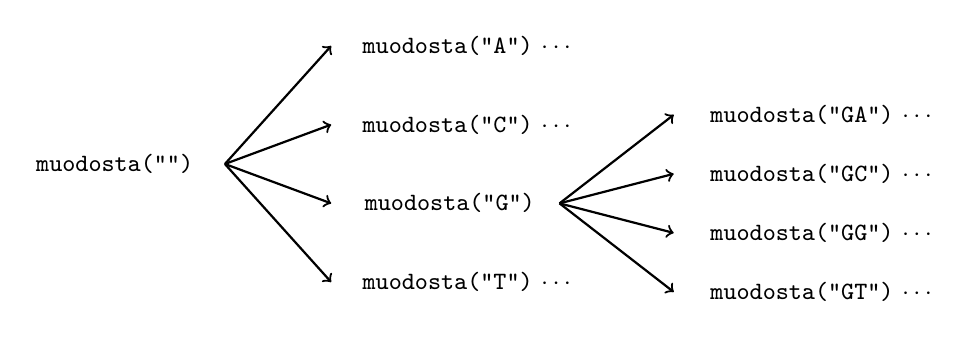
\begin{tikzpicture}[scale=0.5]
\small
\node at (-0.5,0) {\texttt{muodosta("\hspace{0pt}")}};
\node at (8.5,3) {\texttt{muodosta("A")} $\cdots$};
\node at (8.5,1) {\texttt{muodosta("C")} $\cdots$};
\node at (8.5,-1) {\texttt{muodosta("G")} $\phantom{\cdots}$};
\node at (8.5,-3) {\texttt{muodosta("T")} $\cdots$};
\draw[thick,->] (2.3,0) -- (5,3);
\draw[thick,->] (2.3,0) -- (5,1);
\draw[thick,->] (2.3,0) -- (5,-1);
\draw[thick,->] (2.3,0) -- (5,-3);
\node at (17.5,1.25) {\texttt{muodosta("GA")} $\cdots$};
\node at (17.5,-0.25) {\texttt{muodosta("GC")} $\cdots$};
\node at (17.5,-1.75) {\texttt{muodosta("GG")} $\cdots$};
\node at (17.5,-3.25) {\texttt{muodosta("GT")} $\cdots$};
\draw[thick,->] (10.8,-1) -- (13.7,1.25);
\draw[thick,->] (10.8,-1) -- (13.7,-0.25);
\draw[thick,->] (10.8,-1) -- (13.7,-1.75);
\draw[thick,->] (10.8,-1) -- (13.7,-3.25);
\end{tikzpicture}
\caption{DNA-ketjujen muodostaminen rekursiivisesti.}
\label{fig:ketjut}
\end{figure}

Kuva \ref{fig:ketjut} havainnollistaa,
kuinka rekursiivinen aliohjelma lähtee muodostamaan ketjuja.
Ensin aliohjelma haarautuu neljään osaan sen mukaan,
onko ketjun ensimmäinen merkki A, C, G vai T.
Tämän jälkeen haarautuminen jatkuu vastaavasti
jokaisessa kutsussa:
esimerkiksi jos ketju alkaa merkillä G,
rekursio haarautuu tapauksiin GA, GC, GG ja GT, jne.


\subsection{Osajoukkojen läpikäynti}

Joukon osajoukkoja ovat kaikki tavat valita osa joukon alkioista.
Esimerkiksi joukon $\{1,2,3\}$ osajoukot ovat
$\emptyset$ (tyhjä joukko), $\{1\}$, $\{2\}$, $\{3\}$,
$\{1,2\}$, $\{1,3\}$, $\{2,3\}$ ja $\{1,2,3\}$.
Jos joukossa on $n$ alkioita, osajoukkoja on $2^n$.

Rekursio tarjoaa kätevän tavan käydä läpi kaikki
joukon osajoukot. Esimerkiksi seuraava koodi pitää yllä
rakennetta

\begin{code}
ArrayDeque<Integer> osajoukko;
\end{code}

joka sisältää vuorollaan kunkin joukon $\{1,2,\dots,n\}$
osajoukon.
Haku läh\-tee käyntiin, kun kutsumme metodia \texttt{muodosta}
parametrilla $1$.

\begin{code}
void muodosta(int x) {
    if (x == n+1) {
        System.out.println(osajoukko);
        return;
    }
    muodosta(x+1); // x ei valita osajoukkoon
    osajoukko.addLast(x);
    muodosta(x+1); // x valitaan osajoukkoon
    osajoukko.removeLast();
}
\end{code}

Jokaisessa kutsussa metodi käy läpi tapaukset,
otetaanko luku $x$ mukaan osajoukkoon vai ei.
Molemmissa tapauksissa metodi kutsuu itseään yhtä
suuremalla $x$:n arvolla.
Lopulta kun $x=n+1$, kaikki luvut on käyty läpi
ja on aika tulostaa osajoukko.

Esimerkiksi tapauksessa $n=3$ koodin tulostus on seuraava:

\begin{code}
[]
[3]
[2]
[2, 3]
[1]
[1, 3]
[1, 2]
[1, 2, 3]
\end{code}

\subsection{Permutaatioiden läpikäynti}

Joukon permutaatiot ovat kaikki tavat järjestää joukon alkiot.
Esimerkiksi joukon $\{1,2,3\}$ permutaatiot ovat
$(1,2,3)$, $(1,3,2)$, $(2,1,3)$, $(2,3,1)$, $(3,1,2)$ ja $(3,2,1)$.
Jos joukossa on $n$ alkiota, permutaatioita on $n!$.

Myös permutaatioiden läpikäynti onnistuu kätevästi rekursiolla.
Seuraava koodi pitää yllä rakennetta

\begin{code}
ArrayDeque<Integer> permutaatio;
\end{code}

joka sisältää vuorollaan kunkin joukon $\{1,2,\dots,n\}$ permutaation.
Haku lähtee käyntiin, kun kutsumme metodia
\texttt{muodosta} ilman parametreja.

\begin{code}
void muodosta() {
    if (permutaatio.size() == n) {
        System.out.println(permutaatio);
        return;
    }
    for (int i = 1; i <= n; i++) {
        if (!permutaatio.contains(i)) {
            permutaatio.addLast(i);
            muodosta();
            permutaatio.removeLast();
        }
    }
}
\end{code}

Tässä on ideana, että metodi käy joka kutsulla läpi kaikki luvut
$1,2,\dots,n$ ja aina jos luku ei kuulu vielä permutaatioon,
koodi haarautuu rekursiivisesti tapaukseen, jossa se lisätään
seuraavaksi permutaatioon.
Sitten kun permutaatiossa on $n$ lukua, se on valmis ja
voimme tulostaa sen.

Esimerkiksi tapauksessa $n=3$ koodin tulostus on seuraava:

\begin{code}
[1, 2, 3]
[1, 3, 2]
[2, 1, 3]
[2, 3, 1]
[3, 1, 2]
[3, 2, 1]
\end{code}

\subsection{Peruuttava haku}

\emph{Peruuttava haku} on yleinen menetelmä,
jota käyttäen voimme muodostaa järjestelmällisesti
kaikki ratkaisut annettuun tehtävään.
Siinä on ideana aloittaa tyhjästä ratkaisusta ja käydä
joka askeleella läpi rekursiivisesti kaikki mahdolliset tavat laajentaa ratkaisua.

Peruuttava haku on raa'an voiman menetelmä,
ja voimme käyttää sitä vain silloin,
kun ratkaisujen määrä on niin pieni,
että ehdimme käydä kaikki läpi.
Kuitenkin jos voimme käyttää peruuttavaa hakua,
se on mainio tekniikka,
koska voimme olla varmoja, että oikein toteutettu
peruuttava haku löytää kaikki ratkaisut.

\begin{figure}
\center
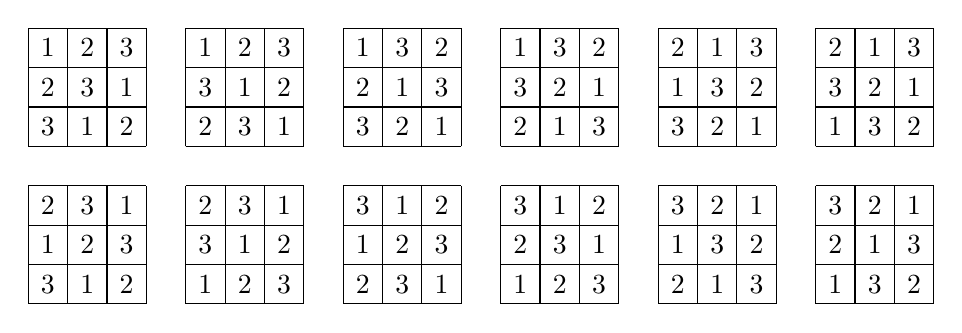
\begin{tikzpicture}[scale=0.5]
\newcommand\nelio[9]{
\draw (0,0) grid (3,3);
\foreach \x/\y/\v in {0/0/#1,1/0/#2,2/0/#3,0/1/#4,1/1/#5,2/1/#6,0/2/#7,1/2/#8,2/2/#9} \node at (0.5+\x,2.5-\y) {\v};
}
\begin{scope}
\nelio{1}{2}{3}{2}{3}{1}{3}{1}{2}
\end{scope}
\begin{scope}[xshift=4cm]
\nelio{1}{2}{3}{3}{1}{2}{2}{3}{1}
\end{scope}
\begin{scope}[xshift=8cm]
\nelio{1}{3}{2}{2}{1}{3}{3}{2}{1}
\end{scope}
\begin{scope}[xshift=12cm]
\nelio{1}{3}{2}{3}{2}{1}{2}{1}{3}
\end{scope}
\begin{scope}[xshift=16cm]
\nelio{2}{1}{3}{1}{3}{2}{3}{2}{1}
\end{scope}
\begin{scope}[xshift=20cm]
\nelio{2}{1}{3}{3}{2}{1}{1}{3}{2}
\end{scope}
\begin{scope}[yshift=-4cm]
\nelio{2}{3}{1}{1}{2}{3}{3}{1}{2}
\end{scope}
\begin{scope}[yshift=-4cm,xshift=4cm]
\nelio{2}{3}{1}{3}{1}{2}{1}{2}{3}
\end{scope}
\begin{scope}[yshift=-4cm,xshift=8cm]
\nelio{3}{1}{2}{1}{2}{3}{2}{3}{1}
\end{scope}
\begin{scope}[yshift=-4cm,xshift=12cm]
\nelio{3}{1}{2}{2}{3}{1}{1}{2}{3}
\end{scope}
\begin{scope}[yshift=-4cm,xshift=16cm]
\nelio{3}{2}{1}{1}{3}{2}{2}{1}{3}
\end{scope}
\begin{scope}[yshift=-4cm,xshift=20cm]
\nelio{3}{2}{1}{2}{1}{3}{1}{3}{2}
\end{scope}
\end{tikzpicture}
\caption{Kaikki 12 latinalaista neliötä kokoa $3 \times 3$.}
\label{fig:latnel}
\end{figure}

Tarkastelemme esimerkkinä tehtävää, jossa haluamme laskea,
montako tietyn kokoista latinalaista neliötä on olemassa.
\emph{Latinalainen neliö} on ruudukko kokoa $n \times n$, jonka
kullakin vaaka- ja pystyrivillä esiintyy tarkalleen kerran
jokainen luku $1,2,\dots,n$.
Kyseessä on siis yksinkertaisempi muoto tutusta sudoku-tehtävästä.
Esimerkiksi kuvassa \ref{fig:latnel} on kaikki 12 latinalaista neliötä kokoa $3 \times 3$.
Kun $n$ kasvaa, niin ratkaisujen määrä kasvaa nopeasti.

Hakua varten määrittelemme seuraavat taulukot:

\begin{code}
int[][] nelio = new int[n][n];
boolean[][] vaaka = new boolean[n][n];
boolean[][] pysty = new boolean[n][n];
\end{code}

Numeroimme ruudukon pysty- ja vaakarivit $0,1,\dots,n-1$.
Tarkoituksena on, että kohdassa $\texttt{nelio}[y][x]$
on neliössä ruudussa $(y,x)$ oleva luku.
Lisäksi $\texttt{vaaka}[y][k]$ kertoo, onko vaakarivillä $y$
jo lukua $k$, ja vastaavasti $\texttt{pysty}[x][k]$ kertoo,
onko pystyrivillä $x$ jo lukua $k$.
Alussa kaikki taulukot ovat tyhjiä ja täytämme niitä
pikkuhiljaa peruuttavan haun aikana.

Seuraava rekursiivinen metodi toteuttaa haun, kun sille
annetaan alkuparametreina $y=0$ ja $x=0$.
Metodi laskee latinalaisten neliöiden määrän muuttujaan 
\texttt{laskuri}.

\begin{code}
void muodosta(int y, int x) {
    if (y == n) laskuri++;
    else if (x == n) muodosta(y+1,0);
    else {
        for (int i = 1; i <= n; i++) {
            if (!vaaka[y][i] && !pysty[x][i]) {
                vaaka[y][i] = pysty[x][i] = true;
                nelio[y][x] = i;
                muodosta(y,x+1);
                vaaka[y][i] = pysty[x][i] = false;
            }
        }
    }
}
\end{code}

Jokaisella askeleella metodi valitsee luvun ruutuun
$(y,x)$ ja siirtyy seuraavaan ruutuun oikealle.
Jos $x=n$, vaakarivi on tullut täyteen ja metodi siirtyy
seuraavalle vaakariville.
Jos taas $y=n$, koko ruudukko on tullut täyteen ja
metodi kasvattaa ruudukoiden määrää yhdellä.

\begin{table}
\center
\begin{tabular}{rr}
ruudukon koko $n$ & neliöiden määrä \\
\hline
1 & 1 \\
2 & 2 \\
3 & 12 \\
4 & 576 \\
5 & 161280 \\
6 & 812851200 \\
\end{tabular}
\caption{Latinalaisten neliöiden määriä pienille $n$:n arvoille.}
\label{tab:latnel}
\end{table}

Tämän koodin avulla voimme laskea latinalaisten neliöiden
määrät ensimmäisille $n$:n arvoille.
Taulukko \ref{tab:latnel} näyttää nämä tulokset.
Suuremmilla $n$:n arvoilla haku alkaa kestää liian kauan
ja meidän tulisi keksiä keino tehostaa hakua,
jos haluaisimme laskea tuloksia suuremmissa tapauksissa.

\section{Matemaattinen tausta}

Tietorakenteiden ja algoritmien teoria perustuu matematiikkaan,
ja käym\-me kirjassa pikkuhiljaa läpi tarvittavia tietoja.
Seuraavassa on joitakin merkintöjä ja käsitteitä, joista on hyötyä
useassa kirjan kohdassa.

\subsection{Summakaavat}

Voimme laskea lukujen $1,2,\dots,n$ summan kaavalla
\[1+2+\dots+n = \frac{n(n+1)}{2}.\]
Esimerkiksi
\[1+2+3+4+5 = \frac{5 \cdot 6}{2}=15.\]
Kaavan voi ymmärtää niin, että laskemme yhteen $n$ lukua,
joiden suuruus on \emph{keskimäärin} $(n+1)/2$.

Toinen hyödyllinen kaava on
\[2^0+2^1+\dots+2^n = 2^{n+1}-1.\]
Esimerkiksi
\[1+2+4+8+16=32-1.\]
Tässä voimme ajatella, että aloitamme luvusta $2^n$
ja lisäämme siihen aina puolet pienemmän luvun lukuun $1$ asti.
Tämän seurauksena pääsemme yhtä vaille lukuun $2^{n+1}$ asti.

Esitämme joskus summia merkinnän $\sum$ avulla.
Siinä on ideana antaa muuttujan ala- ja yläraja sekä
joka askeleella summaan lisättävä arvo.
Esimerkiksi voimme merkitä
\[1^2 + 2^2 + \dots + n^2 = \sum_{i=1}^n i^2.\]

Tämä merkintä on itse asiassa hyvin lähellä ohjelmoinnin
for-silmukkaa, koska seuraava koodi ajaa saman asian:

\begin{code}
int summa = 0;
for (int i = 1; i <= n; i++) {
    summa += i*i;
}
\end{code}

\subsection{Logaritmit}

Logaritmin määritelmän mukaan $\log_b(n)=x$
tarkalleen silloin kun $b^x=n$.
Esimerkiksi $\log_2(32)=5$, koska $2^5=32$.

Algoritmiikassa logaritmin kantaluku $b$ on usein 2,
ja voimme ajatella, että logaritmi kertoo, montako kertaa
meidän tulee \emph{puolittaa} luku $n$, ennen kuin pääsemme lukuun 1.
Esimerkiksi $\log_2(32)=5$, koska tarvitsemme 5 puolitusta:
\[32 \rightarrow 16 \rightarrow 8 \rightarrow 4 \rightarrow 2 \rightarrow 1\]

Logaritmeille pätee kaavat
\[\log_b(x \cdot y) = \log_b(x)+\log_b(y)\]
ja
\[\log_b(x / y) = \log_b(x)-\log_b(y).\]
Ylemmästä kaavasta seuraa myös
\[\log_b(x^k) = k \log_b(x).\]
Lisäksi voimme vaihtaa logaritmin kantalukua kaavalla
\[\log_u(x) = \frac{\log_b(x)}{\log_b(u)}.\]
\chapter{Tehokkuus}

Algoritmien suunnittelussa tavoitteemme on saada aikaan
algoritmeja, jotka toimivat \emph{tehokkaasti}.
Haluamme luoda algoritmeja, joiden avulla voimme
käsitellä myös suuria aineistoja ilman, että joudumme
odottamaan kauan aikaa.
Ajattelemmekin, että algoritmi on \emph{hyvä},
jos se kykenee antamaan meille nopean vastauksen myös silloin,
kun annamme sille paljon tietoa.

Tässä luvussa tutustumme työkaluihin, joiden avulla
voimme arvioida algoritmien tehokkuutta.
Keskeinen käsite on \emph{aikavaativuus}, joka antaa
tiiviissä muodossa kuvan algoritmin ajankäytöstä.
Aikavaativuuden avulla voimme muodostaa pika-arvion
algoritmin tehokkuudesta sen rakenteen perusteella,
eikä meidän tarvitse toteuttaa ja testata algoritmia
vain saadaksemme tietää, miten nopea se on.

\section{Aikavaativuus}

Algoritmin tehokkuus riippuu siitä,
montako askelta se suorittaa.
Tavoitteemme on nyt arvioida tehokkuutta suhteessa
syötteen kokoon $n$.
Esimerkiksi jos syötteenä on taulukko,
$n$ on taulukon koko,
ja jos syötteenä on merkkijono,
$n$ on merkkijonon pituus.

Tarkastellaan esimerkkinä seuraavaa algoritmia,
joka laskee, montako kertaa luku $x$ esiintyy
$n$ lukua sisältävässä taulukossa.

\begin{code}[numbers=left]
int laskuri = 0;
for (int i = 0; i < n; i++) {
    if (luvut[i] == x) {
        laskuri++;
    }
}
\end{code}

Tämän algoritmin oleelliset askeleet ovat riveillä
1, 3 ja 4.
Rivi 1 suoritetaan vain kerran algoritmin alussa.
Rivi 3 suoritetaan $n$ kertaa jokaisella silmukan
kierroksella.
Rivi 4 taas suoritetaan $0 \dots n$
kertaa riippuen siitä, kuinka usein
luku $x$ esiintyy taulukossa.
Algoritmi suorittaa siis vähintään $n+1$ ja enintään $2n+1$
askelta.

Näin tarkka analyysi ei ole kuitenkaan yleensä tarpeen,
vaan meille riittää määrittää karkea ajankäytön yläraja.
Sanomme, että algoritmi toimii ajassa $O(f(n))$ eli sen
\emph{aikavaativuus} on $O(f(n))$, jos se suorittaa
enintään $c f(n)$ askelta aina silloin kun $n \ge n_0$,
missä $c$ ja $n_0$ ovat vakioita.
Esimerkiksi yllä oleva algoritmi toimii ajassa $O(n)$,
koska se suorittaa selkeästi enintään $3n$ askelta
kaikilla $n$:n arvoilla.

Aikavaativuuden mukavana puolena on, että voimme yleensä
päätellä aikavaativuuden helposti algoritmin
rakenteesta. Tutustumme seuraavaksi laskusääntöihin,
joiden avulla tämä on mahdollista.

\subsection{Laskusääntöjä}

Jos koodissa ei ole silmukoita vaan vain
yksittäisiä komentoja, sen aikavaativuus on $O(1)$.
Näin on esimerkiksi seuraavassa koodissa:

\begin{code}
c = a+b;
b = a;
a = c;
\end{code}

Merkitsemme \texttt{...} koodia,
jonka aikavaativuus on $O(1)$.
Jos koodissa on yksi silmukka,
joka suorittaa $n$ askelta,
sen aikavaativuus on $O(n)$:

\begin{code}
for (int i = 0; i < n; i++) {
    ...
}
\end{code}

Jos tällaisia silmukoita on kaksi sisäkkäin,
aikavaativuus on $O(n^2)$:

\begin{code}
for (int i = 0; i < n; i++) {
    for (int j = 0; j < n; j++) {
        ...
    }
}
\end{code}

Yleisemmin jos koodissa on vastaavalla tavalla
$k$ sisäkkäistä silmukkaa, sen aikavaativuus on $O(n^k)$.

Huomaa, että vakiokertoimet ja matalammat termit eivät vaikuta aikavaativuuteen.
Esimerkiksi seuraavissa koodeissa silmukoissa on $2n$ ja $n-1$ askelta,
mutta kummankin koodin aikavaativuus on $O(n)$.

\begin{code}
for (int i = 0; i < 2*n; i++) {
    ...
}
\end{code}

\begin{code}
for (int i = 0; i < n-1; i++) {
    ...
}
\end{code}

Jos koodissa on peräkkäisiä osuuksia, kokonaisaikavaativuus on suurin
yksittäinen aikavaativuus. Esimerkiksi seuraavan koodin aikavaativuus on $O(n^2)$,
koska sen osuudet ovat $O(n)$, $O(n^2)$ ja $O(n)$.

\begin{code}
for (int i = 0; i < n; i++) {
    ...
}
for (int i = 0; i < n; i++) {
    for (int j = 0; j < n; j++) {
        ...
    }
}
for (int i = 0; i < n; i++) {
    ...
}
\end{code}

Joskus aikavaativuus riippuu useammasta tekijästä,
jolloin kaavassa on monta muuttujaa.
Seuraavan koodin aikavaativuus on $O(nm)$:

\begin{code}
for (int i = 0; i < n; i++) {
    for (int j = 0; j < m; j++) {
        ...
    }
}
\end{code}

\subsection{Yleisiä aikavaativuuksia}

Tietyt aikavaativuudet esiintyvät usein algoritmien analyysissa.
Seuraavaksi käymme läpi joukon tällaisia aikavaativuuksia.

\subsubsection{$O(1)$ (vakioaikainen)}

\emph{Vakioaikainen} algoritmi suorittaa kiinteän määrän komentoja,
eikä syötteen suuruus vaikuta algoritmin nopeuteen.
Esimerkiksi seuraava algoritmi laskee summan $1+2+\dots+n$
ajassa $O(1)$ summakaavan avulla:

\begin{code}
summa = n*(n+1)/2;
\end{code}

\subsubsection{$O(\log n)$ (logaritminen)}

\emph{Logaritminen} algoritmi puolittaa usein syötteen koon
joka askeleella. Tyypillinen esimerkki logaritmisesta algoritmista
on binäärihaku, joka etsii alkiota järjestetystä taulukosta.

\begin{code}
int a = 0, b = n-1;
while (a <= b) {
    int k = (a+b)/2;
    if (taulu[k] == x) break;
    if (taulu[k] < x) a = k+1;
    else b = k-1;
}
\end{code}

\subsubsection{$O(n)$ (lineaarinen)}

\emph{Lineaarinen} algoritmi voi käydä läpi syötteen kiinteän määrän kertoja.
Esimerkiksi seuraava algoritmi laskee taulukon lukujen summan $O(n)$-ajassa.

\begin{code}
int summa = 0;
for (int i = 0; i < n; i++) {
    summa += taulu[i];
}
\end{code}

\subsubsection{$O(n \log n)$ (järjestäminen)}

Aikavaativuus $O(n \log n)$ viittaa usein siihen,
että algoritmin osana on \emph{järjes\-tämistä},
koska tehokkaat järjestämisalgoritmit
toimivat ajassa $O(n \log n)$.
Esimerkiksi seuraava $O(n \log n)$-algoritmi laskee,
montako eri alkiota taulukko sisältää.

\begin{code}
Arrays.sort(taulu);
int laskuri = 1;
for (int i = 1; i < n; i++) {
    if (taulu[i] != taulu[i-1]) laskuri++;
}
\end{code}

\subsubsection{$O(n^2)$ (neliöllinen)}

\emph{Neliöllinen} algoritmi voi käydä läpi kaikki tavat valita
kaksi alkiota syötteestä.
Esimerkiksi seuraava $O(n^2)$-algoritmi tutkii, onko taulukossa
kahta lukua, joiden summa on $x$.

\begin{code}
boolean ok = false;
for (int i = 0; i < n; i++) {
    for (int j = i+1; j < n; j++) {
        if (taulu[i]+taulu[j] == x) ok = true;
    }
}
\end{code}

\subsubsection{$O(n^3)$ (kuutiollinen)}

\emph{Kuutiollinen} algoritmi voi käydä läpi kaikki tavat valita
kolme alkiota syöt\-teestä.
Esimerkiksi seuraava $O(n^3)$-algoritmi tutkii, onko taulukossa
kolmea lukua, joiden summa on $x$.

\begin{code}
boolean ok = false;
for (int i = 0; i < n; i++) {
    for (int j = i+1; j < n; j++) {
        for (int k = j+1; k < n; k++) {
            if (taulu[i]+taulu[j]+taulu[k] == x) ok = true;
        }
    }
}
\end{code}

\subsubsection{$O(2^n)$ (osajoukot)}

Aikavaativuus $O(2^n)$ viittaa usein siihen,
että algoritmi käy läpi syötteen osajoukot.
Esimerkiksi alkioiden $\{1,2,3\}$ osajoukot ovat
$\emptyset$, $\{1\}$, $\{2\}$, $\{3\}$, $\{1,2\}$, $\{1,3\}$, $\{2,3\}$ ja $\{1,2,3\}$.

\subsubsection{$O(n!)$ (permutaatiot)}

Aikavaativuus $O(n!)$ viittaa usein siihen,
että algoritmi käy läpi syötteen permutaatiot.
Esimerkiksi alkioiden $\{1,2,3\}$ permutaatiot ovat
$(1,2,3)$, $(1,3,2)$, $(2,1,3)$, $(2,3,1)$, $(3,1,2)$ ja $(3,2,1)$.

\subsection{Tehokkuuden arviointi}

Mitä hyötyä on määrittää algoritmin aikavaativuus?
Hyötynä on, että aikavaativuus antaa meille pika-arvion siitä,
kuinka \emph{hyvä} algoritmi on eli miten suuria syötteitä
sillä voi käsitellä tehokkaasti.
Kun meille kertyy kokemusta algoritmien suunnittelusta,
meille alkaa muodostua selkeä kuva,
mitä eri aikavaativuudet tarkoittavat käytännössä.

Aikavaativuutta voi ajatella samalla tavalla kuin vaikkapa
hotellin tähti\-luokitusta: se kertoo tiiviissä muodossa,
mistä asiassa on kysymys, eikä mei\-dän tarvitse ottaa selvää yksityiskohdista.
Jos meille tarjotaan majoitusta neljän tähden hotellissa,
saamme heti jonkin käsityksen huoneen tasosta,
vaikka emme saisi tarkkaa listausta huoneen varustelusta.
Vastaavasti jos kuulemme, että jonkin algoritmin aikavaativuus on $O(n \log n)$,
voimme heti arvioida karkeasti, miten suuria syötteitä voimme käsitellä,
vaikka emme saisi tarkkaa kuvausta algoritmin toiminnasta.

\begin{table}
\center
\begin{tabular}{rrr}
syötteen koko $n$ & haluttu aikavaativuus \\
\hline
10 & $O(n!)$ \\
20 & $O(2^n)$ \\
500 & $O(n^3)$ \\
5000 & $O(n^2)$ \\
$10^6$ & $O(n)$ tai $O(n \log n)$ \\
suuri & $O(1)$ tai $O(\log n)$ \\
\end{tabular}
\caption{Kuinka suuren syötteen algoritmi voi käsitellä sekunnissa?}
\label{tab:algteh}
\end{table}

Yksi kiinnostava näkökulma algoritmin tehokkuuteen on,
miten suuren syötteen algoritmi voi käsitellä sekunnissa.
Taulukossa \ref{tab:algteh} on joitakin hyödyl\-lisiä arvioita
olettaen, että algoritmi suoritetaan tavallisella nykyaikaisella tietokoneella.
Esimerkiksi jos meillä on $O(n^2)$-algoritmi, voimme käsitellä sillä
tehokkaasti taulukon, jossa on luokkaa 5000 alkiota.
Jos tavoitteemme on käsitellä tehokkaasti suuria syötteitä
(kuten $n=10^6$), meidän tulisi pyrkiä
löytä\-mään $O(n)$- tai $O(n \log n)$-aikainen algoritmi.

Kannattaa silti pitää mielessä, että nämä luvut ovat vain arvioita ja algoritmin
todelliseen ajankäyttöön vaikuttavat monet asiat.
Saman algoritmin hyvä toteutus saattaa olla
kymmenen kertaa nopeampi kuin huono toteutus,
vaikka aikavaativuudet olisivat samat.
Tässä kirjassa analysoimme algoritmeja sekä aikavaativuuksien
avulla että mittaamalla todellisia suoritusaikoja.

\section{Esimerkki: Bittijonot}

Seuraavassa esimerkissä vertailemme kahta
erilaista algoritmia samaan tehtä\-vään.
Ensimmäinen algoritmi on suoraviivainen raa'an voiman
algoritmi, joka toimii ajassa $O(n^2)$.
Toinen algoritmi taas on tehokas algoritmi,
joka toimii ajassa $O(n)$.

Tehtävämme on seuraava: Annettuna on bittijono, jossa on $n$ bittiä,
ja haluamme laskea, monellako tavalla voimme valita kaksi kohtaa
niin, että vasen bitti on 0 ja oikea bitti on 1.
Esimerkiksi bittijonossa 01001 tapoja on neljä:
\underline{01}001, \underline{0}100\underline{1},
01\underline{0}0\underline{1} ja 010\underline{01}.

\subsubsection{$O(n^2)$-ratkaisu}

Voimme ratkaista tehtävän raa'alla voimalla
käymällä läpi kaikki mahdolliset tavat valita vasen ja oikea kohta.
Tällöin voimme laskea yksi kerrallaan,
monessako tavassa vasen bitti on 0 ja oikea bitti on 1.
Seuraava koodi toteuttaa algoritmin olettaen,
että taulukko \texttt{bitit} sisältää $n$ bittiä.

\begin{code}
long tulos = 0;
for (int i = 0; i < n; i++) {
    for (int j = i+1; j < n; j++) {
        if (bitit[i] == 0 && bitit[j] == 1) tulos++;
    }
 }
System.out.println(tulos);
\end{code}

Algoritmin aikavaativuus on $O(n^2)$, koska siinä on kaksi
sisäkkäistä silmukkaa, jotka käyvät läpi syötteen.

\subsubsection{$O(n)$-ratkaisu}

Kuinka voisimme ratkaista tehtävän tehokkaammin?
Meidän tulisi käytän\-nössä keksiä tapa, jolla saisimme
pois toisen silmukan koodista.

Tässä auttaa lähestyä ongelmaa hieman toisesta
näkökulmasta: kun olemme tietyssä kohdassa bittijonoa,
monellako tavalla voimme muodostaa parin,
jonka oikea bitti on nykyisessä kohdassamme?
Jos olemme bitin 0 kohdalla, pareja ei ole yhtään,
mutta jos bittinä on 1, voimme valita minkä tahansa
vasemmalla puolella olevan bitin 0 pariin.

Tämän havainnon ansiosta meidän riittää käydä läpi
bittijono kerran vasemmalta oikealle ja pitää kirjaa,
montako bittiä 0 olemme nähneet.
Sitten jokaisen bitin 1 kohdalla kasvatamme
vastausta tällä bittien 0 määrällä.
Seuraava koodi toteuttaa algoritmin:

\begin{code}
long tulos = 0;
int nollat = 0;
for (int i = 0; i < n; i++) {
    if (bitit[i] == 0) nollat++;
    if (bitit[i] == 1) tulos += nollat;
}
System.out.println(tulos);
\end{code}

Algoritmissa on vain yksi silmukka, joka käy syötteen läpi,
joten sen aikavaativuus on $O(n)$.

\subsubsection{Algoritmien vertailua}

Meillä on nyt siis kaksi algoritmia, joiden aikavaativuudet ovat
$O(n^2)$ ja $O(n)$, mutta mitä tämä tarkoittaa käytännössä?
Tämän selvittämiseksi teemme seuraavaksi testin,
jossa mittaamme algoritmien suoritusaikoja
satunnaisilla syötteillä eri $n$:n arvoilla.

Taulukko \ref{tab:algver} näyttää tällaisen testin tulokset.
Pienillä $n$:n arvoilla molemmat algoritmit toimivat
hyvin tehokkaasti, mutta suuremmilla syötteillä on
nähtävissä huomattavia eroja.
Raakaan voimaan perustuva $O(n^2)$-algoritmi
alkaa hidastua selvästi testistä $n=10000$ alkaen,
ja testissä $n=1000000$ sillä kuluu jo lähes kolme minuuttia aikaa.
Tehokas $O(n)$-algoritmi taas selvittää suuretkin testit
salamannopeasti.

\begin{table}
\center
\begin{tabular}{rrr}
syötteen koko $n$ & $O(n^2)$-algoritmi & $O(n)$-algoritmi \\
\hline
$10$ & 0.00 s & 0.00 s\\
$100$ & 0.00 s & 0.00 s\\
$1000$ & 0.00 s & 0.00 s\\
$10000$ & 0.14 s & 0.00 s \\
$100000$ & 1.66 s & 0.00 s \\
$1000000$ & 172.52 s & 0.01 s \\
\end{tabular}
\caption{Algoritmien suoritusaikojen vertailu.}
\label{tab:algver}
\end{table}

Tämän kurssin jatkuvana teemana on luoda algoritmeja,
jotka toimivat tehokkaasti myös silloin, kun niille annetaan suuria syötteitä.
Tämä tarkoittaa käytännössä sitä, että algoritmin aikavaativuuden tulisi
olla $O(n)$ tai $O(n \log n)$.
Jos algoritmin aikavaativuus on esimerkiksi $O(n^2)$,
se on auttamatta liian hidas suurien syötteiden käsittelyyn.

\section{Lisää algoritmien analysoinnista}

Aikavaativuuksissa esiintyvä $O$-merkintä on yksi monista merkinnöistä,
joiden avulla voimme arvioida funktioiden kasvunopeutta.
Tutustumme seuraavaksi tarkemmin näihin merkintöihin.

\subsection{Merkinnät $O$, $\Omega$ ja $\Theta$}

Algoritmien analysoinnissa usein esiintyviä merkintöjä ovat:

\begin{itemize}
\item \emph{Yläraja}: Funktio $g(n)$ on luokkaa $O(f(n))$, jos on olemassa vakiot $c$ ja $n_0$
niin, että $g(n) \le c f(n)$ aina kun $n \ge n_0$.
\item \emph{Alaraja}: Funktio $g(n)$ on luokkaa $\Omega(f(n))$, jos on olemassa vakiot $c$ ja $n_0$
niin, että $g(n) \ge c f(n)$ aina kun $n \ge n_0$.
\item \emph{Tarkka arvio}: Funktio $g(n)$ on luokkaa $\Theta(f(n))$, jos se on sekä luokkaa $O(f(n))$
että luokkaa $\Omega(f(n))$.
\end{itemize}

Vakion $c$ tarkoituksena on, että saamme arvion kasvunopeuden suuruusluokalle välittämättä
vakiokertoimista. Vakion $n_0$ tarkoituksena on, että keskitymme tarkastelemaan
kasvunopeutta suurilla $n$:n arvoilla.
Voimme myös kirjoittaa $g(n)=O(f(n))$, kun haluamme ilmaista,
että funktio $g(n)$ on luokkaa $O(f(n))$,
ja vastaavasti $\Omega$- ja $\Theta$-merkinnöissä.

Kun sanomme, että algoritmi toimii ajassa $O(f(n))$, tarkoitamme, että se suorittaa
\emph{pahimmassa tapauksessa} $O(f(n))$ askelta.
Tämä on yleensä hyvä tapa ilmoittaa algoritmin tehokkuus,
koska silloin annamme takuun siitä, että algoritmin ajankäytöllä on tietty yläraja,
vaikka syöte olisi valittu mahdollisimman ikävästi algoritmin kannalta.

Tarkastellaan esimerkkinä seuraavaa algoritmia, joka laskee
taulukon lukujen summan:

\begin{code}
int summa = 0;
for (int i = 0; i < n; i++) {
    summa += taulu[i];
}
\end{code}

Tämä algoritmi toimii samalla tavalla riippumatta taulukon sisällöstä,
koska se käy aina läpi koko taulukon.
Niinpä yläraja ajankäytölle on $O(n)$ ja alaraja ajankäytölle on samoin $\Omega(n)$,
joten voimme sanoa, että algoritmi vie aikaa $\Theta(n)$ kaikissa tapauksissa.

Tarkastellaan sitten seuraavaa algoritmia, joka selvittää,
onko taulukossa lukua $x$:

\begin{code}
ok = false;
for (int i = 0; i < n; i++) {
    if (taulu[i] == x) {
        ok = true;
        break;
    }
}
\end{code}

Tässä algoritmin pahin ja paraus tapaus eroavat.
Ajankäytön yläraja on $O(n)$, koska algoritmi joutuu käymään
läpi kaikki taulukon alkiot silloin, kun luku $x$
ei esiinny taulukossa.
Toisaalta ajankäytön alaraja on $\Omega(1)$,
koska jos luku $x$ on taulukon ensimmäinen alkio,
algoritmi pysähtyy heti taulukon alussa.
Voimme myös sanoa, että algoritmi suorittaa pahimmassa
tapauksessa $\Theta(n)$ askelta ja parhaassa tapauksessa
$\Theta(1)$ askelta.

Tärkeä huomio on, että $O$-merkinnän antama yläraja voi olla
\emph{mikä tahansa} yläraja, ei välttämättä tarkka yläraja.
On siis oikein sanoa esimerkiksi, että äskeinen
algoritmi vie aikaa $O(n^2)$, vaikka on olemassa parempi yläraja $O(n)$.
Miksi sitten käytämme $O$-merkintää, vaikka voisimme usein myös ilmaista tarkan
ajankäytön $\Theta$-merkinnällä?
Tämä on vakiintunut ja käytännössä toimiva tapa.
Olisi hyvin harhaanjohtavaa antaa algoritmille yläraja $O(n^2)$,
jos näemme suoraan, että aikaa kuluu vain $O(n)$.

Asiaa voi ajatella niin, että $O$-merkintää käytetään algoritmin
\emph{markkinoinnissa}. Jos annamme liian suuren ylärajan, algoritmista
tulee väärä käsitys yleisölle.
Vertauksena jos myymme urheiluautoa, jonka huippunopeus on 250 km/h,
on sinänsä paikkansa pitävä väite, että autolla pystyy ajamaan 100 km/h.
Meidän ei kuitenkaan kannata antaa tällaista vähättelevää tietoa,
vaan kertoa, että autolla pystyy ajamaan 250 km/h.

\subsection{Tilavaativuus}

Merkintöjä $O$, $\Omega$ ja $\Theta$ voi käyttää
kaikenlaisissa yhteyksissä, ei vain algoritmin ajankäytön arvoinnissa.
Esimerkiksi voimme sanoa, että algoritmi suorittaa silmukkaa $O(\log n)$ kierrosta
tai että taulukossa on $O(n^2)$ lukua.

Aikavaativuuden lisäksi kiinnostava tieto algoritmista on sen
\emph{tilavaativuus}. Tämä tarkoittaa yleensä sitä, miten paljon algoritmi
käyttää muistia syötteen \emph{lisäksi}.
Jos tilavaativuus on $O(1)$, algoritmi tarvitsee muistia
vain yksittäisille muuttujille syötteen lisäksi.
Jos tilavaativuus on $O(n)$, algoritmi voi varata esimerkiksi aputaulukon,
jonka koko vastaa syötteen kokoa.

Tarkastellaan esimerkkinä tehtävää, jossa meille annetaan taulukko,
joka sisältää luvut $1,2,\dots,n$ yhtä lukuun ottamatta,
ja tehtävämme on selvittää puuttuva luku.
Yksi tapa ratkaista tehtävä $O(n)$-ajassa on luoda aputaulukko,
joka pitää kirjaa mukana olevista luvuista.
Tällaisen ratkaisun tilavaativuus on $O(n)$,
koska aputaulukko vie $O(n)$ muistia.

\begin{code}
boolean[] mukana = new boolean[n+1];
for (int i = 0; i < n-1; i++) {
    mukana[taulu[i]] = true;
}
for (int i = 1; i <= n; i++) {
    if (!mukana[i]) puuttuva = i;
}
\end{code}

Tehtävään on kuitenkin olemassa myös toinen algoritmi,
jossa aikavaativuus on edelleen $O(n)$ mutta tilavaativuus on vain $O(1)$.
Tällainen algoritmi laskee ensin lukujen $1,2,\dots,n$ summan
ja vähentää sitten taulukossa esiintyvät luvut siitä.
Jäljelle jäävä luku on puuttuva luku.

\begin{code}
int summa = 0;
for (int i = 1; i <= n; i++) {
    summa += i;
}
for (int i = 0; i < n-1; i++) {
    summa -= taulu[i];
}
puuttuva = summa;
\end{code}

Käytännössä tilavaativuus on yleensä sivuroolissa algoritmeissa,
koska jos algoritmi vie vain vähän aikaa, se ei \emph{ehdi} käyttää kovin paljon muistia.
Erityisesti tilavaativuus ei voi olla suurempi kuin aikavaativuus.
Niinpä meidän riittää tavallisesti keskittyä suunnittelemaan algoritmeja,
jotka toimivat nopeasti, ja vertailla algoritmien aikavaativuuksia.

\subsection{Rajojen todistaminen}

Jos haluamme todistaa täsmällisesti, että jokin raja pätee,
meidän täytyy löytää vakiot $c$ ja $n_0$, jotka osoittavat asian.
Jos taas haluamme todistaa, että raja ei päde,
meidän täytyy näyttää, että mikään vakioiden $c$ ja $n_0$ valinta ei ole kelvollinen.

Jos haluamme todistaa rajan pätemisen,
tämä onnistuu yleensä helposti valitsemalla vakio $c$
tarpeeksi suureksi ja arvioimalla summan osia ylöspäin tarvittaessa.
Esimerkiksi jos haluamme todistaa, että $3n+5 = O(n)$, meidän tulee löytää
vakiot $c$ ja $n_0$, joille pätee, että $3n+5 \le cn$ aina kun $n \ge n_0$.
Tässä tapauksessa voimme valita esimerkiksi $c=8$ ja $n_0=1$,
jolloin voimme arvioida $3n+5 \le 3n+5n=8n$, kun $n \ge 1$.

Jos haluamme todistaa, että raja ei päde, tilanne on hankalampi,
koska meidän täytyy näyttää, että ei ole olemassa \emph{mitään} kelvollista
tapaa valita vakioita $c$ ja $n_0$.
Tässä auttaa tyypillisesti vastaoletuksen tekeminen: oletamme,
että raja pätee ja voimme valita vakiot,
ja näytämme sitten, että tämä oletus johtaa ristiriitaan.

Todistetaan esimerkkinä, että $n^2 \neq O(n)$.
Jos pätisi $n^2=O(n)$, niin olisi olemassa vakiot $c$ ja $n_0$,
joille $n^2 \le cn$ aina kun $n \ge n_0$.
Voimme kuitenkin osoittaa, että tämä aiheuttaa ristiriidan.
Jos $n^2 \le cn$, niin voimme jakaa epäyhtälön molemmat puolet $n$:llä
ja saamme $n \le c$.
Tämä tarkoittaa, että $n$ on aina enintään yhtä suuri kuin vakio $c$.
Tämä ei ole kuitenkaan mahdollista, koska $n$ voi olla miten
suuri tahansa, joten ei voi päteä $n^2 = O(n)$.

Määritelmistä lähtevä todistaminen on sinänsä mukavaa ajanvietettä,
mutta sille on äärimmäisen harvoin tarvetta käytännössä,
kun haluamme tutkia algoritmien tehokkuutta.
Voimme koko kurssin ajan huoletta päätellä algoritmin aikavaativuuden
katsomalla, mikä sen rakenne on, kuten olemme tehneet tämän luvun alkuosassa.
\chapter{Järjestäminen}

\section{Perusalgoritmit}

\section{Tehokkaat algoritmit}

\subsection{Lomitusjärjestäminen}

\subsection{Pikajärjestäminen}

\subsection{Laskemisjärjestäminen}

\section{Järjestäminen Javassa}

\section{Ongelmanratkaisu}

\chapter{Lista}

Ohjelmoinnin perustietorakenne on taulukko,
joka on mainio tietorakenne, mutta siinä on yksi puute.
Kun luomme taulukon, meidän täytyy antaa sille
kiinteä koko, emmekä voi muuttaa kokoa myöhemmin.
Esimerkiksi seuraava koodi luo taulukon,
jossa on kiinteästi kymmenen alkiota:

\begin{code}
int[] taulu = new int[10];
\end{code}

Tämä on ongelma, koska meillä ei välttämättä ole
taulukon luontihetkellä käsitystä, montako alkiota
haluaisimme tallentaa siihen myöhemmin.

Tämän luvun tavoitteemme on luoda tietorakenne,
joka muistuttaa taulukkoa, mutta 
voimme lisätä ja poistaa alkioita jälkeenpäin.
Kutsumme tietorakennetta nimellä \emph{lista}.
Tutustumme kahteen tapaan listan toteuttamiseen,
joissa molemmissa on omat hyvät ja huonot puolensa.

\section{Taulukkolista}

\emph{Taulukkolista} on lista, joka on tallennettu taulukkoon.
Esimerkiksi seuraava koodi luo taulukon,
joka vastaa listaa $[3,7,2,5]$:

\begin{code}
int[] lista = {3,7,2,5};
\end{code}

Ongelmana on kuitenkin, kuinka voisimme muuttaa
taulukkoon tallennetun listan kokoa.
Löydämme ongelmaan pian ratkaisun, mutta sitä ennen
aiheellinen kysymys on:
miksi Javan suunnittelijat ovat olleet niin keljuja,
että he eivät lisänneet taulukkoon mahdollisuutta
muuttaa sen kokoa?

Tähän on hyvä selitys, ja se liittyy siihen,
miten taulukko on tallennettu tietokoneen muistissa.
Tarkastellaan esimerkkinä seuraavaa koodia:

\begin{code}
int[] a = {1,4,2};
int[] b = {5,3,2,5};
\end{code}

\begin{figure}
\center
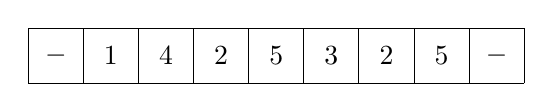
\begin{tikzpicture}[scale=0.7]
\draw (0,0) grid (9,1);
\node at (0.5,0.5) {$-$};
\node at (1.5,0.5) {$1$};
\node at (2.5,0.5) {$4$};
\node at (3.5,0.5) {$2$};
\node at (4.5,0.5) {$5$};
\node at (5.5,0.5) {$3$};
\node at (6.5,0.5) {$2$};
\node at (7.5,0.5) {$5$};
\node at (8.5,0.5) {$-$};
\end{tikzpicture}
\caption{Taulukot $[1,4,2]$ ja $[5,3,2,5]$ tietokoneen muistissa.}
\label{fig:taumui}
\end{figure}

Kuva \ref{fig:taumui} näyttää mahdollisen tavan, miten taulukot
\texttt{a} ja \texttt{b} asettuvat muistissa.
Taulukossa \texttt{a} on kolme alkiota,
joten sille on varattu kolme paikkaa muistista,
ja taulukossa \texttt{b} on neljä alkiota,
joten sille on varattu neljä paikkaa muistista.
Taulukolle varataan aina yhtenäinen muistialue,
minkä ansiosta pääsemme käsiksi sen alkioihin
helposti ajassa $O(1)$.

Tästä seuraa ilmeinen syy,
minkä vuoksi emme voi laajentaa taulukon kokoa
luonnin jälkeen:
tyypillisesti muistissa on heti taulukon perässä muuta
tarpeellista tietoa, jota ei saa poistaa.
Jos lisäisimme taulukon \texttt{a} perään uuden alkion,
meidän täytyisi tuhota taulukon \texttt{b} ensimmäinen alkio,
mikä ei tule kysymykseen.
Ainoa tapa laajentaa taulukkoa onkin varata
jostain muualta muistista enemmän tilaa ja kopioida
taulukon sisältö sinne.
Juuri näin joudumme tekemään, kun toteutamme listan taulukkona.

\subsection{Muutokset lopussa}

Toteutamme ensin taulukkolistan, jossa voimme
lisätä ja poistaa alkioita listan lopussa.
Tallennamme listan taulukkona niin,
että tietty määrä alkioita taulukon alussa on listan käytössä
ja loput alkiot on varattu tuleville alkioille.
Tämän ansiosta pystymme lisäämään uuden alkion listalle
ajassa $O(1)$, jos taulukossa on tilaa,
koska meidän riittää ottaa käyttöön seuraava
vapaana oleva kohta taulukosta.

Kuva \ref{fig:listau} näyttää esimerkin,
jossa taulukossa on tilaa yhteenä kahdeksalle alkiolle
ja siihen on tallennettu lista $[3,7,2,5]$.
Taulukon neljä ensimmäistä alkiota on siis listan käytössä,
ja muut ovat varalla tulevia alkioita varten.
Kun lisäämme listan loppuun uuden alkion 6,
otamme käyttöön taulukosta uuden kohdan, johon alkio sijoitetaan.

\begin{figure}
\center
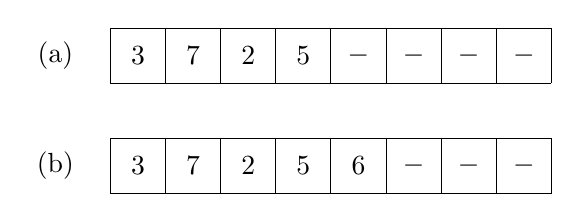
\begin{tikzpicture}[scale=0.7]
\begin{scope}
\draw (0,0) grid (8,1);
\node at (-1,0.5) {(a)};
\node at (0.5,0.5) {$3$};
\node at (1.5,0.5) {$7$};
\node at (2.5,0.5) {$2$};
\node at (3.5,0.5) {$5$};
\node at (4.5,0.5) {$-$};
\node at (5.5,0.5) {$-$};
\node at (6.5,0.5) {$-$};
\node at (7.5,0.5) {$-$};
\end{scope}
\begin{scope}[yshift=-2cm]
\draw (0,0) grid (8,1);
\node at (-1,0.5) {(b)};
\node at (0.5,0.5) {$3$};
\node at (1.5,0.5) {$7$};
\node at (2.5,0.5) {$2$};
\node at (3.5,0.5) {$5$};
\node at (4.5,0.5) {$6$};
\node at (5.5,0.5) {$-$};
\node at (6.5,0.5) {$-$};
\node at (7.5,0.5) {$-$};
\end{scope}
\end{tikzpicture}
\caption{(a) Lista $[3,7,2,5]$ tallennettuna taulukkoon. (b) Listan loppuun lisätään alkio 6.}
\label{fig:listau}
\end{figure}

\begin{figure}
\center
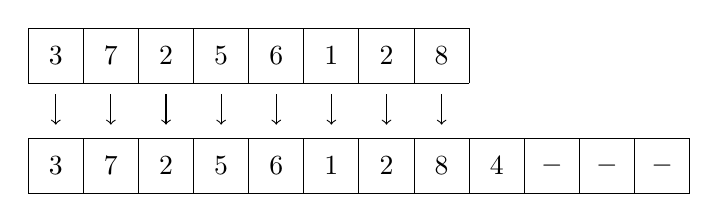
\begin{tikzpicture}[scale=0.7]
\begin{scope}
\draw (0,0) grid (8,1);
\node at (0.5,0.5) {$3$};
\node at (1.5,0.5) {$7$};
\node at (2.5,0.5) {$2$};
\node at (3.5,0.5) {$5$};
\node at (4.5,0.5) {$6$};
\node at (5.5,0.5) {$1$};
\node at (6.5,0.5) {$2$};
\node at (7.5,0.5) {$8$};
\foreach \x in {0,...,7} \draw[->] (\x+0.5,-0.2) -- (\x+0.5,-0.75);
\end{scope}
\begin{scope}[yshift=-2cm]
\draw (0,0) grid (12,1);
\node at (0.5,0.5) {$3$};
\node at (1.5,0.5) {$7$};
\node at (2.5,0.5) {$2$};
\node at (3.5,0.5) {$5$};
\node at (4.5,0.5) {$6$};
\node at (5.5,0.5) {$1$};
\node at (6.5,0.5) {$2$};
\node at (7.5,0.5) {$8$};
\node at (8.5,0.5) {$4$};
\node at (9.5,0.5) {$-$};
\node at (10.5,0.5) {$-$};
\node at (11.5,0.5) {$-$};
\end{scope}
\end{tikzpicture}
\caption{Taulukkoon ei mahdu enää uutta alkiota. Meidän täytyy varata uusi suurempi taulukko
ja kopioida vanhan taulukon sisältö sinne.}
\label{fig:lisuus}
\end{figure}

Mitä tapahtuu sitten, kun jossain vaiheessa koko taulukko
on täynnä eikä uusi listalle lisättävä alkio mahdu enää taulukkoon?
Tällöin meidän täytyy ensin varata uusi suurempi taulukko ja
kopioida kaikki vanhan taulukon alkiot siihen.
Vasta tämän jälkeen voimme lisätä uuden alkion listalle.
Tämä vie aikaa $O(n)$, koska kopioimme kaikki listan alkiot
uuteen paikkaan muistissa.
Esimerkiksi kuvassa \ref{fig:lisuus} uusi alkio 4 ei mahdu taulukkoon,
joten joudumme varaamaan uuden taulukon ja kopioimaan alkiot.

Olemme saaneet siis aikaan listan, jossa lisääminen
vie aikaa \emph{joko} $O(1)$ tai $O(n)$ riippuen siitä,
mahtuuko alkio nykyiseen taulukkoon vai täytyykö
meidän varata uusi taulukko.
Jotta lista olisi käyttökelpoinen, hidas $O(n)$-operaatio
ei saisi esiintyä liian usein.
Osoittautuu, että saavutamme tämän tavoitteen,
kunhan varaamme uuden taulukon aina reilusti aiempaa suuremmaksi.
Tavanomainen ratkaisu on \emph{kaksinkertaistaa} taulukon koko aina,
kun varaamme uuden taulukon.
Kun toimimme näin, jokaisen alkion lisääminen listalle vie
\emph{keskimäärin} vain $O(1)$ aikaa.

Voimme ajatella asian näin: jokainen listalle lisättävä alkio
maksaa \emph{pääsy\-maksuna} kolme euroa.
Tästä yksi euro menee listalle liittymiseen ja kaksi euroa jäävät säästöön.
Sitten kun aikanaan listalle täytyy varata suurempi taulukko,
jokainen viime erässä lisätty alkio maksaa yhden euron omasta siirrostaan
ja yhden euron aiemmin lisätyn alkion siirrosta.
Koska taulukon koko kaksinkertaistuu joka vaiheessa,
kolmen euron kiinteä pääsymaksu riittää siihen, että kaikki tulevat
siirrot saadaan kustannettua.

\begin{figure}
\center
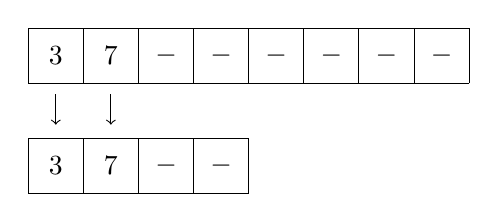
\begin{tikzpicture}[scale=0.7]
\begin{scope}
\draw (0,0) grid (8,1);
\node at (0.5,0.5) {$3$};
\node at (1.5,0.5) {$7$};
\node at (2.5,0.5) {$-$};
\node at (3.5,0.5) {$-$};
\node at (4.5,0.5) {$-$};
\node at (5.5,0.5) {$-$};
\node at (6.5,0.5) {$-$};
\node at (7.5,0.5) {$-$};
\foreach \x in {0,...,1} \draw[->] (\x+0.5,-0.2) -- (\x+0.5,-0.75);
\end{scope}
\begin{scope}[yshift=-2cm]
\draw (0,0) grid (4,1);
\node at (0.5,0.5) {$3$};
\node at (1.5,0.5) {$7$};
\node at (2.5,0.5) {$-$};
\node at (3.5,0.5) {$-$};
\end{scope}
\end{tikzpicture}
\caption{Poistojen jälkeen taulukon koko on käynyt tarpeettoman suureksi,
ja puolitamme taulukon koon.}                                                                        
\label{fig:lispoi}
\end{figure}

Voimme poistaa alkion listan lopusta aina $O(1)$-ajassa,
koska taulukon kokoa ei tarvitse koskaan suurentaa.
Tässä voi kuitenkin tulla ongelmaksi, että monien poistojen
jälkeen taulukossa on turhan paljon tyhjää tilaa lopussa.
Voimme soveltaa tässä käänteisesti samaa ideaa kuin lisäämisessä:
jos poistamisen jälkeen vain \emph{neljännes} taulukosta on käytössä,
puolitamme taulukon koon.
Kuva \ref{fig:lispoi} näyttää esimerkin tällaisesta tilanteesta.
Tällä tavalla poistamiset vievät keskimäärin aikaa $O(1)$.

Miksi sitten emme voisi varata heti aluksi niin suurta taulukkoa,
että lopullinen lista mahtuisi siihen varmasti?
Tässä olisi huonona puolena, että listamme tuhlaisi paljon muistia.
Ohjelmassa saattaa olla samaan aikaan käytössä monia listoja,
ja haluamme, että listalle varattu taulukko on samaa kokoluokkaa
kuin listan todellinen sisältö.

\subsection{Muutokset alussa ja lopussa}

Melko samaan tapaan voimme myös luoda taulukkolistan,
joka sallii tehokkaat alkioiden lisäykset ja poistot
sekä listan alussa että lopussa.
Jotta tämä onnistuisi, muutamme listan tallennustapaa niin,
että lista voi alkaa ja päättyä missä tahansa taulukon
kohdassa ja listan sisältö voi jatkua taulukon lopusta alkuun.
Tämän ansiosta pystymme tekemään lisäyksiä ja poistoja
listan molemmissa päissä.

\begin{figure}
\center
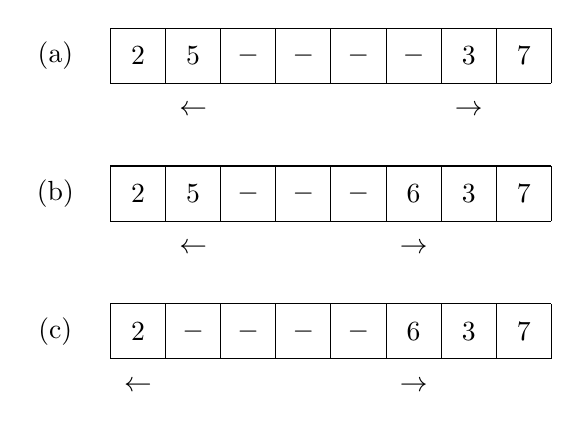
\begin{tikzpicture}[scale=0.7]
\begin{scope}
\draw (0,0) grid (8,1);
\node at (-1,0.5) {(a)};
\node at (0.5,0.5) {$2$};
\node at (1.5,0.5) {$5$};
\node at (2.5,0.5) {$-$};
\node at (3.5,0.5) {$-$};
\node at (4.5,0.5) {$-$};
\node at (5.5,0.5) {$-$};
\node at (6.5,0.5) {$3$};
\node at (7.5,0.5) {$7$};
\node at (1.5,-0.5) {$\leftarrow$};
\node at (6.5,-0.5) {$\rightarrow$};
\end{scope}
\begin{scope}[yshift=-2.5cm]
\draw (0,0) grid (8,1);
\node at (-1,0.5) {(b)};
\node at (0.5,0.5) {$2$};
\node at (1.5,0.5) {$5$};
\node at (2.5,0.5) {$-$};
\node at (3.5,0.5) {$-$};
\node at (4.5,0.5) {$-$};
\node at (5.5,0.5) {$6$};
\node at (6.5,0.5) {$3$};
\node at (7.5,0.5) {$7$};
\node at (1.5,-0.5) {$\leftarrow$};
\node at (5.5,-0.5) {$\rightarrow$};
\end{scope}
\begin{scope}[yshift=-5cm]
\draw (0,0) grid (8,1);
\node at (-1,0.5) {(c)};
\node at (0.5,0.5) {$2$};
\node at (1.5,0.5) {$-$};
\node at (2.5,0.5) {$-$};
\node at (3.5,0.5) {$-$};
\node at (4.5,0.5) {$-$};
\node at (5.5,0.5) {$6$};
\node at (6.5,0.5) {$3$};
\node at (7.5,0.5) {$7$};
\node at (0.5,-0.5) {$\leftarrow$};
\node at (5.5,-0.5) {$\rightarrow$};
\end{scope}
\end{tikzpicture}
\caption{(a) Lista $[3,7,2,5]$ tallennettuna taulukkoon.
(b) Listan alkuun lisätään alkio 6.
(c) Listan lopusta poistetaan alkio 5.}
\label{fig:lismol}
\end{figure}

Kuva \ref{fig:lismol} näyttää esimerkin listan $[3,7,2,5]$
uudesta tallennustavasta.
Merkki $\rightarrow$ osoittaa kohdan, josta lista alkaa,
ja merkki $\leftarrow$ osoittaa kohdan, johon lista päättyy.
Kun haluamme lisätä alkion listan alkuun,
siirrymme vasemmalle kohdasta $\rightarrow$,
ja kun haluamme lisätä alkion listan loppuun,
siirrymme oikealle kohdasta $\leftarrow$.
Kun haluamme poistaa alkioita listasta,
menettelemme käänteisesti.

\begin{figure}
\center
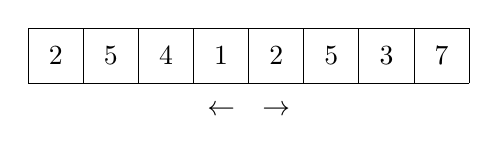
\begin{tikzpicture}[scale=0.7]
\begin{scope}
\draw (0,0) grid (8,1);
\node at (0.5,0.5) {$2$};
\node at (1.5,0.5) {$5$};
\node at (2.5,0.5) {$4$};
\node at (3.5,0.5) {$1$};
\node at (4.5,0.5) {$2$};
\node at (5.5,0.5) {$5$};
\node at (6.5,0.5) {$3$};
\node at (7.5,0.5) {$7$};
\node at (3.5,-0.5) {$\leftarrow$};
\node at (4.5,-0.5) {$\rightarrow$};
\end{scope}
\end{tikzpicture}
\caption{Lista $[2,5,3,7,2,5,4,1]$ täyttää koko taulukon, emmekä voi lisätä uutta alkiota.
Ratkaisuna on varata suurempi taulukko.}
\label{fig:lismol2}
\end{figure}

Jos kohdat $\rightarrow$ ja $\leftarrow$ ovat vierekkäin,
taulukko on täynnä, emmekä voi enää lisätä uutta alkiota
listan alkuun tai loppuun.
Kuva \ref{fig:lismol2} näyttää esimerkin tällaisesta tilanteesta.
Tällöin meidän täytyy varata uusi suurempi taulukko,
johon listan sisältö siirretään.
Voimme menetellä samalla tavalla kuin aiemmin ja
kaksinkertaistaa taulukon koon joka vaiheessa,
jolloin operaatiot vievät keskimäärin aikaa $O(1)$.

\section{Linkitetty lista}

\emph{Linkitetty lista} muodostuu solmuista, joista jokainen sisältää
yhden listan alkion.
Yhteen suuntaan linkitetyssä listassa jokaisessa
solmussa on viittaus listan seuraavaan solmuun.
Kahteen suuntaan linkitetyssä listassa taas
solmut viittaavat sekä listan seuraavaan että edelliseen solmuun.
Viittausten avulla pystymme liikkumaan listassa.

\begin{figure}
\center
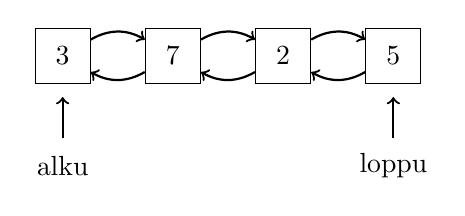
\begin{tikzpicture}[scale=0.7]
\begin{scope}
\node[draw, rectangle, minimum size=7mm] (1) at (0,0) {$3$};
\node[draw, rectangle, minimum size=7mm] (2) at (2,0) {$7$};
\node[draw, rectangle, minimum size=7mm] (3) at (4,0) {$2$};
\node[draw, rectangle, minimum size=7mm] (4) at (6,0) {$5$};
\path[draw,thick,->] (1) edge [bend left] (2);
\path[draw,thick,->] (2) edge [bend left] (3);
\path[draw,thick,->] (3) edge [bend left] (4);
\path[draw,thick,->] (4) edge [bend left] (3);
\path[draw,thick,->] (3) edge [bend left] (2);
\path[draw,thick,->] (2) edge [bend left] (1);
\node at (0,-2) {alku};
\node at (6,-2) {loppu};
\path[draw,thick,->] (0,-1.5) -- (0,-0.75);
\path[draw,thick,->] (6,-1.5) -- (6,-0.75);
\end{scope}
\end{tikzpicture}
\caption{Kahteen suuntaan linkitetty lista, joka sisältää alkiot $[3,7,2,5]$.}
\label{fig:linlis}
\end{figure}

Kuvassa \ref{fig:linlis} on esimerkkinä kahteen suuntaan linkitetty lista,
joka sisältää alkiot $[3,7,2,5]$.
Jokainen alkio viittaa seuraavaan ja edelliseen alkioon,
minkä ansiosta pystymme liikkumaan listassa.
Lisäksi tiedossamme on viittaukset listan alkuun ja loppuun.
Voimme esimerkiksi käydä listan läpi aloittamalla alusta
ja siirtymällä aina seuraavaan solmuun askel kerrallaan.

Kaksisuuntainen linkitys on käytännössä järkevä tapa toteuttaa
linkitetty lista, ja oletamme jatkossa, että listamme on
kahteen suuntaan linkitetty ja meillä on tiedossa viittaukset
listan alkuun ja loppuun.

\subsection{Linkitetyt rakenteet}

Jokaisessa ohjelmointikielessä on omat keinonsa
linkitetyn rakenteen toteuttamiseen.
Javassa voimme toteuttaa linkitetyn rakenteen niin,
että jokainen solmu on oma olionsa.
Esimerkiksi voimme toteuttaa seuraavan luokan \texttt{Solmu},
jonka oliot toimivat linkitetyn listan solmuina:

\begin{code}
public class Solmu {
    public int arvo;
    public Solmu seuraava;
    public Solmu edellinen;

    public Solmu(int arvo, Solmu seuraava, Solmu edellinen) {
        this.arvo = arvo;
        this.seuraava = seuraava;
        this.edellinen = edellinen;
    }
}
\end{code}

Tässä kenttä \texttt{arvo} kertoo solmun arvon,
kenttä \texttt{seuraava} osoittaa seuraavaan solmuun
ja kenttä \texttt{edellinen} osoittaa edelliseen solmuun.
Jos seuraavaa tai edellistä solmua ei ole,
viittauksen tilalla on arvo \texttt{null}.
Tämän luokan avulla voisimme luoda linkitetyn listan $[3,7,2,5]$
seuraavasti:

\begin{code}
Solmu s1, s2, s3, s4;
s1 = new Solmu(3, s2, null);
s2 = new Solmu(7, s3, s1);
s3 = new Solmu(2, s4, s2);
s4 = new Solmu(5, null, s3);
\end{code}

Tämän jälkeen voisimme käydä listan läpi näin alusta loppuun:

\begin{code}
Solmu s = s1;
while (s != null) {
    System.out.println(s.arvo);
    s = s.seuraava;
}
\end{code}

Koodin tulostus on seuraava:

\begin{code}
3
7
2
5
\end{code}

\subsection{Listan operaatiot}

Linkitetyn listan etuna on,
että voimme lisätä ja poistaa
alkioita $O(1)$-ajassa kaikissa listan kohdissa.
Kun haluamme lisätä listalle alkion,
luomme ensin uuden solmun ja muutamme sitten
sen vieressä olevien solmujen viittauksia niin,
että ne viittaavat uuteen solmuun.
Vastaavasti kun haluamme poistaa alkion,
muutamme viittauksia niin, että solmu ohitetaan.

\begin{figure}
\center
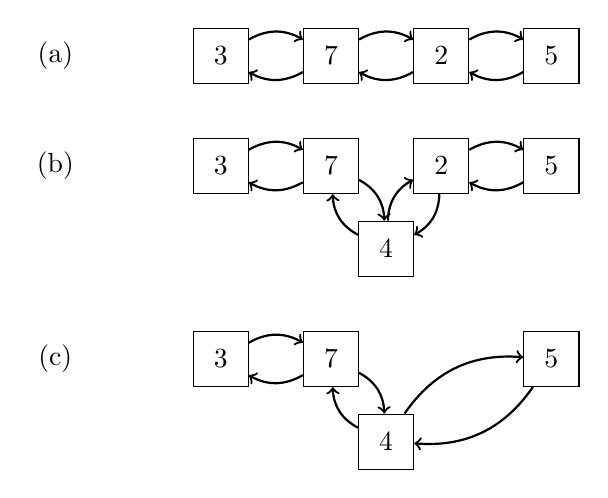
\begin{tikzpicture}[scale=0.7]
\begin{scope}
\node at (-3,0) {(a)};
\node[draw, rectangle, minimum size=7mm] (1) at (0,0) {$3$};
\node[draw, rectangle, minimum size=7mm] (2) at (2,0) {$7$};
\node[draw, rectangle, minimum size=7mm] (3) at (4,0) {$2$};
\node[draw, rectangle, minimum size=7mm] (4) at (6,0) {$5$};
\path[draw,thick,->] (1) edge [bend left] (2);
\path[draw,thick,->] (2) edge [bend left] (3);
\path[draw,thick,->] (3) edge [bend left] (4);
\path[draw,thick,->] (4) edge [bend left] (3);
\path[draw,thick,->] (3) edge [bend left] (2);
\path[draw,thick,->] (2) edge [bend left] (1);
\end{scope}
\begin{scope}[yshift=-2cm]
\node at (-3,0) {(b)};
\node[draw, rectangle, minimum size=7mm] (1) at (0,0) {$3$};
\node[draw, rectangle, minimum size=7mm] (2) at (2,0) {$7$};
\node[draw, rectangle, minimum size=7mm] (3) at (4,0) {$2$};
\node[draw, rectangle, minimum size=7mm] (4) at (6,0) {$5$};
\node[draw, rectangle, minimum size=7mm] (5) at (3,-1.5) {$4$};
\path[draw,thick,->] (1) edge [bend left] (2);
\path[draw,thick,->] (2) edge [bend left] (5);
\path[draw,thick,->] (5) edge [bend left] (3);
\path[draw,thick,->] (3) edge [bend left] (4);
\path[draw,thick,->] (4) edge [bend left] (3);
\path[draw,thick,->] (3) edge [bend left] (5);
\path[draw,thick,->] (5) edge [bend left] (2);
\path[draw,thick,->] (2) edge [bend left] (1);
\end{scope}
\begin{scope}[yshift=-5.5cm]
\node at (-3,0) {(c)};
\node[draw, rectangle, minimum size=7mm] (1) at (0,0) {$3$};
\node[draw, rectangle, minimum size=7mm] (2) at (2,0) {$7$};
\node[draw, rectangle, minimum size=7mm] (4) at (6,0) {$5$};
\node[draw, rectangle, minimum size=7mm] (5) at (3,-1.5) {$4$};
\path[draw,thick,->] (1) edge [bend left] (2);
\path[draw,thick,->] (2) edge [bend left] (5);
\path[draw,thick,->] (5) edge [bend left] (4);
\path[draw,thick,->] (4) edge [bend left] (5);
\path[draw,thick,->] (5) edge [bend left] (2);
\path[draw,thick,->] (2) edge [bend left] (1);
\end{scope}
\end{tikzpicture}
\caption{(a) Alkuperäinen lista $[3,7,2,5]$.
(b) Listan keskelle lisätään alkio $4$.
(c) Listasta poistetaan alkio $2$.}
\label{fig:lismuu}
\end{figure}

Kuva \ref{fig:lismuu} näyttää esimerkin linkitetyn listan käsittelystä.
Listan sisältönä on aluksi $[3,7,2,5]$.
Sitten lisämme listan keskelle alkion 4,
jolloin luomme ensin uuden solmun alkiolle ja muutamme
sitten viittauksia alkioiden 7 ja 2 välillä niin,
että alkio 4 tulee niiden väliin.
Lopuksi poistamme listasta alkion 2, jolloin yhdistämme
alkiot 4 ja 5 suoraan toisiinsa.

Koska meillä on muistissa viittaukset listan alkuun ja loppuun,
pääsemme niihin solmuihin tehokkaasti.
Sen sijaan jos haluamme päästä johonkin muuhun listan kohtaan,
meidän tulee aloittaa alusta tai lopusta ja kulkea askel
kerrallaan viittauksia seuraten.
Niinpä tiettyyn listan kohtaan pääseminen vie aikaa $O(n)$.
Joudumme tekemään näin, koska listan alkiot ovat muistissa
sekalaisissa kohdissa eikä meillä ole suoraa keinoa päästä niihin.

\subsection{Toteutusten vertailua}

\begin{table}
\center
\begin{tabular}{lrr}
operaatio & taulukkolista & linkitetty lista \\
\hline
pääsy listan alkuun & $O(1)$ & $O(1)$ \\
pääsy listan loppuun & $O(1)$ & $O(1)$ \\ 
pääsy listan keskelle &  $O(1)$ & $O(n)$ \\
lisäys/poisto listan alussa & $O(1)^*$ & $O(1)$ \\
lisäys/poisto listan lopussa & $O(1)^*$ & $O(1)$ \\ 
lisäys/poisto listan keskellä &  $O(n)$ & $O(1)$ \\
\end{tabular}
\caption{Taulukkolistan ja linkitetyn listan operaatioiden
aikavaativuuksia. Merkintä $^*$ tarkoittaa keskimääräistä aikavaativuutta.}
\label{tab:taulin}
\end{table}

Taulukko \ref{tab:taulin} esittää yhteenvedon taulukkolistan ja
linkitetyn listan ominaisuuksista.
Kummassakin toteutuksessa on yksi operaatio,
joka ei ole tehokas.
Taulukkolistassa pääsemme tehokkaasti mihin tahansa listan
kohtaan, mutta on hidasta muokata listaa keskeltä.
Linkitetyssä listassa voimme muokata listaa mistä tahansa,
mutta keskelle pääseminen on hidasta.

Huomaa, että keskelle pääsemisen hitaus rajoittaa melko paljon
linkitetyn listan käyttämistä.
Vaikka pystymme sinänsä muokkaamaan listaa mistä tahansa kohdasta
tehokkaasti, meidän tulee ensin \emph{päästä} kyseiseen kohtaan.
Jos meillä on jostain syystä etukäteen tiedossa viittaus listan keskelle,
voimme muokata kyseistä kohtaa tehokkaasti,
mutta muuten meidän tulee ensin kulkea haluttuun kohtaan,
missä kuluu aikaa $O(n)$.

\section{Javan toteutukset}

Javan standardikirjastossa on monia listojen toteutuksia,
jotka pohjautuvat taulukkolistaan tai linkitettyyn listaan.
Seuraavaksi tutustumme rakenteisiin, joista on usein
hyötyä algoritmien toteutuksessa.

\subsection{\texttt{ArrayList}-rakenne}

\texttt{ArrayList}-rakenne on taulukkolista,
joka sallii tehokkaat lisäykset ja poistot listan lopussa.
Esimerkiksi seuraava koodi luo listan, lisää siihen alkiot
1, 2 ja 3 ja tulostaa listan sisällön.

\begin{code}
ArrayList<Integer> lista = new ArrayList<>();
lista.add(1);
lista.add(2);
lista.add(3);
System.out.println(lista); // [1, 2, 3]
\end{code}

Metodi \texttt{add} toimii keskimäärin ajassa $O(1)$,
joten voimme lisätä tehokkaasti alkioita listan loppuun.

Koska lista on tallennettu taulukkona,
pääsemme myös tehokkaasti käsiksi sen alkioihin
kohdan perusteella.
Metodi \texttt{get} hakee tietyssä kohdassa olevan arvon,
ja metodi \texttt{set} muuttaa arvoa.
Esimerkiksi seuraava koodi tulostaa ensin
listan kohdassa 1 olevan alkion ja muuttaa sitten
sen arvoksi 5.

\begin{code}
System.out.println(lista.get(1)); // 2
lista.set(1,5);
System.out.println(lista); // [1, 5, 3]
\end{code}

Luokassa \texttt{Collections} on hyödyllisiä metodeita
listan käsittelyyn.
Seuraava koodi järjestää ensin listan,
muuttaa sitten sen järjestyksen käänteiseksi
ja sekoittaa lopuksi järjestyksen.

\begin{code}
Collections.sort(lista);
Collections.reverse(lista);
Collections.shuffle(lista);
\end{code}

\subsection{\texttt{ArrayDeque}-rakenne}

\texttt{ArrayDeque}-rakenne on taulukkolista,
joka sallii tehokkaat lisäykset ja poistot
sekä listan alussa että lopussa.
Alkioita voi lisätä
metodeilla \texttt{addFirst} ja \texttt{addLast}
ja poistaa
metodeilla \texttt{removeFirst} ja \texttt{removeLast}.

\begin{code}
ArrayDeque<Integer> lista = new ArrayDeque<>();
lista.addLast(1);
lista.addFirst(2);
lista.addLast(3);
System.out.println(lista); // [2, 1, 3]
lista.removeFirst();
System.out.println(lista); // [1, 3]
\end{code}

Lisäksi voimme hakea listan ensimmäisen ja viimeisen
alkion metodeilla \texttt{getFirst} ja \texttt{getLast}.

\begin{code}
System.out.println(lista.getFirst()); // 1
System.out.println(lista.getLast()); // 3
\end{code}

Kaikki nämä metodit toimivat keskimäärin ajassa $O(1)$.
Rajoituksena on kuitenkin, että emme pääse käsiksi
listan keskellä oleviin alkioihin, vaan voimme käsitellä
vain listan alkua ja loppua.

\subsection{\texttt{LinkedList}-rakenne}

\texttt{LinkedList}-rakenne toteuttaa kaksisuuntaisen
linkitetyn listan, jossa voimme helposti lisätä ja poistaa
alkioita listan alussa ja lopussa.
Seuraava koodi esittelee asiaa:

\begin{code}
LinkedList<Integer> lista = new LinkedList<>();
lista.addLast(1);
lista.addFirst(2);
lista.addLast(3);
System.out.println(lista); // [2, 1, 3]
lista.removeFirst();
System.out.println(lista); // [1, 3]
\end{code}

Jos haluamme tehdä lisäyksiä ja poistoja muualla listassa,
meidän täytyy ottaa käyttöön \emph{iteraattori}, joka osoittaa haluttuun kohtaan.
Seuraava koodi luo iteraattorin, joka osoittaa ensin listan alkuun.
Sitten siirrämme iteraattoria kaksi askelta eteenpäin ja
lisäämme alkion 5 iteraattorin kohdalle eli listan
toisen ja kolmannen alkion väliin.

\begin{code}
ListIterator<Integer> x = lista.listIterator(0);
x.next();
x.next();
x.add(5);
\end{code}

\texttt{LinkedList} tarjoaa myös metodit
\texttt{get} ja \texttt{set}, joiden avulla
pääsemme käsiksi tietyssä kohdassa listalla olevaan alkioon.
Nämä metodit vievät kuitenkin aikaa $O(n)$,
koska joudumme kulkemaan ensin oikeaan kohtaan listan
alusta tai lopusta.
Tämän vuoksi \texttt{LinkedList} ei ole hyvä valinta,
jos haluamme käsitellä alkioita kohdan perusteella.

\section{Tehokkuusvertailu}

Tärkeä kysymys on, miten tehokkaita taulukkolista ja
linkitetty lista ovat \emph{käytännössä} ja kumpaa meidän
kannattaa käyttää, jos voimme valita.
Seuraavaksi vertailemme Javan taulukkolistan
(\texttt{ArrayList}) ja linkitetyn listan (\texttt{LinkedList})
käytännön tehokkuutta.

Suoritamme kaksi testiä, joista ensimmäisessä mittaamme
listan luomisen tehokkuutta ja toisessa listan läpikäynnin tehokkuutta.
Jokaisessa testissä toistamme testin kymmenen kertaa ja laskemme
suoritusaikojen keskiarvon, jotta saamme luotettavampia tuloksia.

Sekä \texttt{ArrayList} että \texttt{LinkedList}
toteuttavat rajapinnan \texttt{List},
joten voimme käyttää listaa samalla tavalla kummankin
rakenteen testaamisessa.
Määrittelemme listan seuraavilla tavoilla testistä riippuen:

\begin{code}
List<Integer> lista = new ArrayList<>();
\end{code}

\begin{code}
List<Integer> lista = new LinkedList<>();
\end{code}

\subsubsection{Ensimmäinen testi: listan luominen}

Ensimmäisessä testissä tutkimme, kauanko vie aikaa luoda lista
aloittamalla tyhjästä listasta ja lisäämällä alkioita yksi kerrallaan.
Lisäämme testissä listalle alkiot $1,2,\dots,n$.
Seuraava koodi toteuttaa testin:

\begin{code}
for (int i = 1; i <= n; i++) {
    lista.add(i);
}
\end{code}

% \begin{table}
% \center
% \begin{tabular}{rrr}
% parametri $n$ & \texttt{ArrayList} & \texttt{LinkedList} \\
% \hline
% $10^6$ & 0.03 s & 0.04 s \\
% $2 \cdot 10^6$ & 0.11 s & 0.28 s \\
% $4 \cdot 10^6$ & 0.14 s & 2.08 s \\
% $8 \cdot 10^6$ & 1.76 s & 5.09 s \\
% $16 \cdot 10^6$ & 4.02 s & 12.69 s \\
% \end{tabular}
% \caption{Algoritmien suoritusaikojen vertailu.}
% \label{tab:lispoi}
% \end{table}

TODO testin tulokset

\subsubsection{Toinen testi: listan läpikäynti}

Toisessa testissä tutkimme, kauanko vie aikaa käydä lista läpi.
Tässä testissä meillä on valmiina lista,
jossa on $n$ lukua, ja laskemme lukujen summan.
Seuraava koodi toteuttaa testin:

\begin{code}
long summa = 0;
for (Integer x : lista) {
    summa += x;
}
\end{code}

TODO testin tulokset

\subsubsection{Milloin käyttää linkitettyä listaa?}

Jokaisessa tietorakenteessa on omat hyvät ja huonot puolensa,
ja kaikille on tietyt käyttötarkoituksensa.
Linkitetty lista muodostaa kuitenkin poikkeuksen tähän sääntöön:
on äärimmäisen harvoja tilanteita, jolloin sitä kannattaisi
käyttää taulukkolistan sijasta.

\begin{figure}
\center
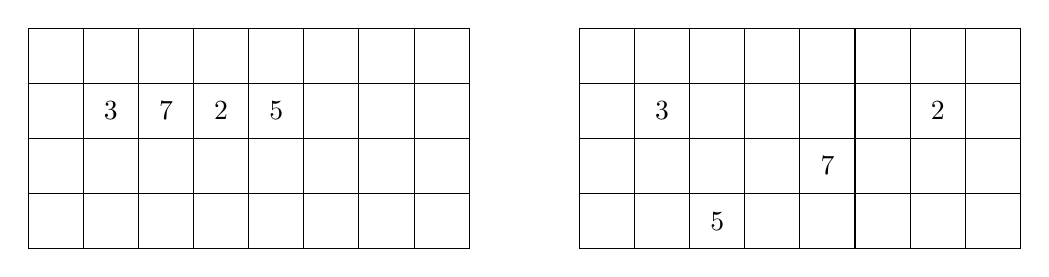
\begin{tikzpicture}[scale=0.7]
\begin{scope}
\draw (0,0) grid (8,4);
\node at (1.5,2.5) {3};
\node at (2.5,2.5) {7};
\node at (3.5,2.5) {2};
\node at (4.5,2.5) {5};
\end{scope}
\begin{scope}[xshift=10cm]
\draw (0,0) grid (8,4);
\node at (1.5,2.5) {3};
\node at (4.5,1.5) {7};
\node at (6.5,2.5) {2};
\node at (2.5,0.5) {5};
\end{scope}
\end{tikzpicture}
\caption{Taulukkolista ja linkitetty lista tietokoneen muistissa.}
\label{fig:taulin}
\end{figure}

Syynä tähän on, että nykyaikaiset tietokoneet
\emph{suosivat} taulukkolistan käyttämistä linkitetyn listan sijaan.
Kuvassa \ref{fig:taulin} näkyy, miten taulukkolista ja linkitetty lista
asettuvat tietokoneen muistissa.
Taulukkolistan alkiot ovat peräkkäin, kun taas linkitetyn
listan alkiot voivat olla eri puolilla muistia sekalaisessa
järjestyksessä.
Nykyaikaisen prosessorin välimuistit ja komentojen ennustus
on toteutettu niin, että ne ovat parhaimmillaan silloin,
kun tieto on tallennettu muistissa peräkkäin -- eli juuri kuten
taulukkolistassa.
Tämä näkyy käytännössä siinä, että taulukkolistan käsittely on selvästi
nopeampaa kuin linkitetyn listan käsittely.
\chapter{Hajautustaulu}

\section{Hajautuksen teoriaa}

\emph{Hajautustaulu} on tietorakenne, jonka avulla voi
pitää yllä tehokkaasti joukkoa alkioista.
Hajautustaulu toteutetaan taulukkona, jonka jokaisessa
kohdassa on lista alkioista.
Lisäksi tarvitsemme \emph{hajautusfunktion},
jonka avulla voimme laskea mille tahansa alkiolle
\emph{hajautusarvon} eli mihin kohtaan hajautustaulua
alkio tallennetaan.

Kuvassa X on esimerkkinä hajautustaulu, jossa on
merkkijonot \texttt{apina}, \texttt{banaani} ja \texttt{cembalo}.
Tässä hajautustaulussa on kymmenen mahdollista kohtaa
($0,1,\ldots,9$), joihin voi tallentaa alkioita.
Merkkijonojen \texttt{apina} ja \texttt{cembalo}
hajautusarvo on 2, joten ne ovat samassa listassa kohdassa 2.
Merkkijonon \texttt{banaani} hajautusarvo on 7,
joten se on yksin omassa listassaan.
Kaikki muut hajautustaulun listat ovat tällä hetkellä tyhjiä.

Kun olemme luoneet hajautustaulun, voimme tarkistaa,
onko tietty alkio taulussa, laskemalla sen hajautusarvon
ja käymällä läpi vastaavan listan.
Vastaavasti voimme lisätä alkion hajautustauluun
lisäämällä sen vastaavan listan loppuun ja poistaa
alkion hajautustaulusta poistamalla sen listasta.
Näiden operaatioiden aikavaativuus on $O(k)$,
missä $k$ on yksittäisen listan pituus,
koska meidän täytyy käydä läpi hajautusarvoa vastaava lista.
Hajautustaulun tehokkuus riippuu siis siitä,
kuinka pitkiä listat ovat.

\subsection{Hajautusarvon laskeminen}

Hajautusfunktio määrittää, mihin kohtaan hajautustaulua
alkio sijoitetaan.
Sen täytyy antaa jokaiselle mahdolliselle alkiolle
hajautusarvo eli kokonaisluvu väliltä $0,1,\ldots,n-1$,
missä $n$ on hajautustaulun koko,
mutta meillä on muuten vapaat kädet hajautusfunktion suunnitteluun.
Ainoa välttämätön vaatimus on, että tietty alkio saa aina
saman hajautusarvon, jotta voimme löytää sen uudelleen
hajautustaulusta.

Jotta hajautustaulu olisi käyttökelpoinen, hajautusfunktioon
liittyy kuitenkin toinenkin vaatimus:
sen tulisi jakaa alkiot mahdollisimman \emph{tasaisesti}
eri puolille hajautustaulua.
Syynä tähän on, että hajautustaulun tehokkuus riippuu siitä,
miten tasaisesti alkiot ovat jakautuneet.
Jos alkiot ovat jakautuneet tasaisesti ja listat ovat lyhyitä,
voimme etsiä alkioita ja päivittää hajautustaulua tehokkaasti.

Merkkijonojen tapauksessa yksi mahdollinen hajautusfunktio
palauttaa merkkijonon pituuden.
Tällöin esimerkiksi merkkijono \texttt{apina} saa
hajautusarvon 5 ja merkkijono \texttt{banaani} saa
hajautusarvon 7.
Tällainen hajautusfunktio on sinänsä toimiva,
mutta sen huonona puolena on, että se antaa monelle
merkkijonolle saman hajautusarvon.
Esimerkiksi suomen kielessä on suuri määrä 5-kirjaimisia
sanoja ja ne kaikki saavat saman hajautusarvon tätä
hajautusfunktiota käyttämällä.

Kehittyneempi hajautusfunktio merkkijonoja varten
ottaa huomioon myös merkkijonon sisällön.
Esimerkiksi voimme sopia, että merkki \texttt{a} vastaa
lukua 1, merkki \texttt{b} vastaa lukua 2, jne.
Tämän jälkeen voimme käyttää hajautusarvona merkkijonon
merkkien koodien summaa.
Nyt esimerkiksi merkkijonon \texttt{apina} hajautusarvo
on $1+16+9+14+1=41$.
Tämä on selvästi parempi hajautusfunktio,
mutta ongelmana on vielä se, että jos kahdessa
merkkijonossa on samat merkit eri järjestyksessä,
ne saavat saman hajautusarvon.

Voimme parantaa hajautusfunktiota asettamalla eri
kohdissa oleville merkeille eri kertoimet.
Yleinen tapa on \emph{polynominen hajautus},
jossa kertoimet valitaan niin, että ne ovat muotoa
$A^k$, missä $A$ on vakio ja $k$ on merkin paikka
merkkijonossa lopusta lukien.
Esimerkiksi jos $A=3$, merkkijonon \texttt{apina}
hajautusarvoksi tulee
\[ 1\cdot3^4+16\cdot3^3+9\cdot3^2+14\cdot3^1+1\cdot3^0 = 637.\]

Polynominen hajautus on käytännössä hyvin toimiva tapa
määrittää hajautusarvo, ja se on käytössä esimerkiksi
Javan standardikirjastossa.

\subsection{Hajautustaulun tehokkuus}

\section{Hajautus Javassa}

Javassa on kaksi hajautustaulua käyttävää tietorakennetta:
\texttt{HashSet} ylläpitää tehokkaasti joukkoa alkioista
ja \texttt{HashMap} on yleistetty taulukko,
jossa voi olla avaimina minkä tahansa tyyppisiä alkioita.
Seuraavaksi tutustumme tarkemmin näihin rakenteisiin.

\subsection{\texttt{HashSet}}

Javan \texttt{HashSet}-rakenne pitää yllä joukkoa alkioista
hajautustaulun avulla.
Rakenteen tärkeimmät operaatiot ovat seuraavat:

\begin{itemize}
\item $\texttt{add}(x)$: lisää alkio $x$ joukkoon
\item $\texttt{contains}(x)$: tarkasta, onko alkio $x$ joukossa
\item $\texttt{remove}(x)$: poista alkio $x$ joukosta
\item $\texttt{size}()$: laske, montako alkiota on joukossa
\end{itemize}

Esimerkiksi seuraava koodi luo joukon, jossa voi olla
kokonaislukuja, ja lisää luvut 3, 5 ja 8 joukkoon.
Tämän jälkeen koodi tulostaa joukon sisällön.

\begin{code}
HashSet<Integer> joukko = new HashSet<Integer>();
joukko.add(3);
joukko.add(5);
joukko.add(8);
System.out.println(joukko); // [3, 5, 8]
\end{code}

Huomaa, että jokainen alkio voi esiintyä vain kerran joukossa.
Esimerkiksi vaikka seuraava koodi lisää luvun 5 kolmesti
joukkoon, se menee sinne vain ensimmäisellä kerralla ja
muut lisäykset jätetään huomiotta.

\begin{code}
HashSet<Integer> joukko = new HashSet<Integer>();
joukko.add(5);
joukko.add(5);
joukko.add(5);
System.out.println(joukko); // [5]
\end{code}

Olennainen seikka \texttt{HashSet}-rakenteessa on,
että operaatiot \texttt{add}, \texttt{contains} ja \texttt{remove}
toimivat kaikki keskimäärin tehokkaasti ajassa $O(1)$
hajautustaulun ansiosta.
Niinpä voimme tehdä mitä tahansa muutoksia ja hakuja
rakenteeseen ja koodi toimii nopeasti.
Tämä ei olisi mahdollista \texttt{ArrayList}-rakenteessa,
jossa operaatiot \texttt{contains} ja \texttt{remove}
vievät aikaa $O(n)$.

\subsection{\texttt{HashMap}}

\texttt{HashMap}-rakenne pitää yllä joukkoa avain-arvo-pareja.
Rakennetta voi ajatella taulukon yleistyksenä:
$n$ alkion taulukossa avaimet ovat aina kokonaisluvut
$0,1,\ldots,n-1$, mutta \texttt{HashMap} sallii
avaimina minkä tahansa tyyppisiä alkioita eikä niiden
tarvitse olla peräkkäisiä kokonaislukuja.

Esimerkiksi seuraava koodi luo sanakirjan, jossa sekä
avaimet että arvot ovat merkkijonoja.
Sanakirjaan voi syöttää merkkijonopareja, jotka kertovat
sanan käännöksen suomesta englanniksi.
Metodi \texttt{put} lisää uuden avain-arvo-parin,
ja metodi \texttt{get} hakee arvon avaimen perusteella.

\begin{code}
HashMap<String,String> sanakirja = new HashMap<String,String>();

sanakirja.put("apina","monkey");
sanakirja.put("banaani","banana");
sanakirja.put("cembalo","harpsichord");

System.out.println(sanakirja.get("banaani")); // banana
\end{code}

Hyödyllinen on myös metodi \texttt{containsKey},
jonka avulla voi tarkastaa, onko tietylle avaimelle
tallennettu arvoa:

\begin{code}
if (sanakirja.containsKey(sana)) {
    System.out.println("Käännös: " + sanakirja.get(sana));
} else {
    System.out.println("Sana puuttuu sanakirjasta!");
}
\end{code}

Koska \texttt{HashMap} on toteutettu hajautustaulun avulla,
sen operaatiot toimivat tehokkaasti keskimäärin $O(1)$-ajassa.

\subsection{Metodi \texttt{hashCode}}

Javan hajautustaulut perustuvat siihen, että olioissa
on metodi \texttt{hashCode}, jonka avulla olio kertoo
pyydettäessä hajautusarvonsa.
Voimme esimerkiksi selvittää merkkijonon \texttt{"ABC"}
hajautusarvon näin:

\begin{code}
System.out.println("ABC".hashCode());
\end{code}

Tämä koodi tulostaa luvun 64578,
joka on siis merkkijonon \texttt{"ABC"} hajautusarvo Javassa.

Metodi \texttt{hashCode} on toteutettu valmiiksi Javan
sisäisiin tyyppeihin, kuten \texttt{Integer} ja \texttt{String},
joten voimme käyttää niitä suoraan hajautustauluissa.
Kuitenkin jos meillä on itse tehty luokka, jonka olioita
haluamme käyttää hajautustauluissa, meidän on toteutettava
itse metodi \texttt{hashCode}.

Esimerkiksi jos meillä on luokka \texttt{Asiakas},
jossa on kenttinä merkkijonot
\texttt{etunimi} ja \texttt{sukunimi},
voisimme toteuttaa metodin \texttt{hashCode} seuraavasti:

\begin{code}
public class Asiakas {
    private String etunimi;
    private String sukunimi;

    int hashCode() {
        return etunimi.hashCode()+sukunimi.hashCode();
    }

    // ...
}
\end{code}

\chapter{Binäärihakupuu}

\index{binäärihakupuu}

\emph{Binäärihakupuu} (\emph{binary search tree})
on tietorakenne, joka pitää yllä
alkioiden joukkoa, samaan tapaan kuin hajautustaulu.
Binäärihakupuu eroaa hajautustaulusta kuitenkin siinä,
että se säilyttää alkioita \emph{järjestyksessä}.
Tämän ansiosta voimme esimerkiksi etsiä tehokkaasti
joukon pienimmän tai suurimman alkion,
mikä ei ole mahdollista hajautustaulussa.

Aloitamme luvun tutustumalla binääripuiden teoriaan,
minkä jälkeen perehdymme binäärihakupuun toimintaan.
Käsittelemme binäärihakupuun tehokkaasta toteutuksesta
esimerkkinä AVL-puun.
Sitten käymme läpi Javan tietorakenteet
\texttt{TreeSet} ja \texttt{TreeMap}, jotka
perustuvat binäärihakupuuhun,
ja lopuksi vertailemme joukkorakenteita ja järjestämistä.

\section{Taustaa binääripuista}

\index{binääripuu}

Binäärihakupuun taustalla on yleisempi tietorakenne \emph{binääripuu}
(\emph{binary tree}).
Ennen kuin tutustumme binäärihakupuuhun,
meidän onkin hyvä selvittää ensin, mikä on binääripuu ja mitä
ominaisuuksia siihen liittyy.

\index{juuri}
\index{lapsi}
\index{vanhempi}
\index{lehti}

Binääripuu muodostuu $n$ solmusta.
Puussa ylimpänä on solmu, jota kutsutaan \emph{juureksi} (\emph{root}).
Jokaisella solmulla voi olla vasen ja oikea \emph{lapsi} (\emph{child}),
ja kaikilla solmuilla juurta lukuun ottamatta on yksikäsitteinen
\emph{vanhempi} (\emph{parent}).
Puun \emph{lehtiä} (\emph{leaf}) ovat solmut, joilla ei ole lapsia.

\index{alipuu}

Binääripuun rakenne on rekursiivinen:
jokainen solmu toimii juurena \emph{alipuulle} (\emph{subtree}),
joka on myös binääripuu.
Solmun $x$ alipuu sisältää solmun $x$ sekä kaikki
solmut, joihin pääsemme laskeutumalla alaspäin solmusta $x$.
Voimme myös ajatella asiaa niin, että jokaisen binääripuun
solmun vasen ja oikea lapsi on toinen (mahdollisesti tyhjä) binääripuu.

\begin{figure}
\center
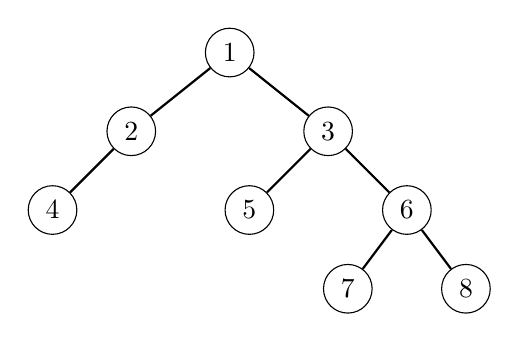
\begin{tikzpicture}[scale=0.5]
\node[draw, circle] (1) at (0,0) {$1$};
\node[draw, circle] (2) at (-2.5,-2) {$2$};
\node[draw, circle] (3) at (2.5,-2) {$3$};
\node[draw, circle] (4) at (-4.5,-4) {$4$};
\node[draw, circle] (5) at (0.5,-4) {$5$};
\node[draw, circle] (6) at (4.5,-4) {$6$};
\node[draw, circle] (7) at (3,-6) {$7$};
\node[draw, circle] (8) at (6,-6) {$8$};
\path[draw,thick,-] (1) -- (2);
\path[draw,thick,-] (1) -- (3);
\path[draw,thick,-] (2) -- (4);
\path[draw,thick,-] (3) -- (5);
\path[draw,thick,-] (3) -- (6);
\path[draw,thick,-] (6) -- (7);
\path[draw,thick,-] (6) -- (8);
\end{tikzpicture}
\caption{Binääripuu, jossa on 8 solmua. Puun juuri on solmu 1,
ja puun lehtiä ovat solmut 4, 5, 7 ja 8.}
\label{fig:binpuu}
\end{figure}

Kuvassa \ref{fig:binpuu} on esimerkki binääripuusta, jossa on 8 solmua.
Solmu 1 on puun juuri, ja solmut 4, 5, 7 ja 8 ovat puun lehtiä.
Solmun 3 vasen lapsi on solmu 5, oikea lapsi on solmu 6
ja vanhempi on solmu 1.
Solmun 3 alipuu sisältää solmut 3, 5, 6, 7 ja 8.

Binääripuun juuren \emph{syvyys} (\emph{depth}) on 0 ja jokaisen muun solmun syvyys on yhtä
suurempi kuin sen vanhemman syvyys.
Binääripuun \emph{korkeus} (\emph{height}) on puolestaan
suurin puun solmussa esiintyvä syvyys
eli toisin sanoen suurin askelten määrä juuresta alaspäin lehteen.
Esimerkiksi kuvan \ref{fig:binpuu} puun korkeus on 3,
koska solmujen 7 ja 8 syvyys on 3.

\begin{figure}
\center
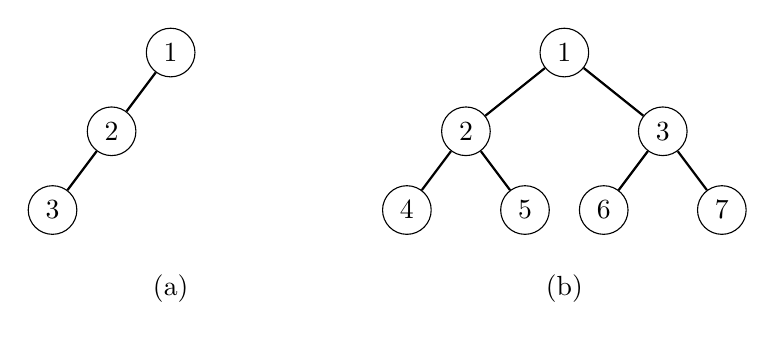
\begin{tikzpicture}[scale=0.5]
\begin{scope}
\node[draw, circle] (1) at (0,0) {$1$};
\node[draw, circle] (2) at (-1.5,-2) {$2$};
\node[draw, circle] (3) at (-3,-4) {$3$};
\path[draw,thick,-] (1) -- (2);
\path[draw,thick,-] (2) -- (3);
\node at (0,-6) {(a)};
\end{scope}
\begin{scope}[xshift=10cm]
\node[draw, circle] (1) at (0,0) {$1$};
\node[draw, circle] (2) at (-2.5,-2) {$2$};
\node[draw, circle] (3) at (2.5,-2) {$3$};
\node[draw, circle] (4) at (-4,-4) {$4$};
\node[draw, circle] (5) at (-1,-4) {$5$};
\node[draw, circle] (6) at (1,-4) {$6$};
\node[draw, circle] (7) at (4,-4) {$7$};
\path[draw,thick,-] (1) -- (2);
\path[draw,thick,-] (1) -- (3);
\path[draw,thick,-] (2) -- (4);
\path[draw,thick,-] (2) -- (5);
\path[draw,thick,-] (3) -- (6);
\path[draw,thick,-] (3) -- (7);
\node at (0,-6) {(b)};
\end{scope}
\end{tikzpicture}
\caption{(a) Vähiten solmuja sisältävä korkeuden 2 binääripuu.
(b) Eniten solmuja sisältävä korkeuden 2 binääripuu.}
\label{fig:binraj}
\end{figure}

Jos binääripuun korkeus on $h$, siinä on vähintään $h+1$ solmua,
jolloin puu on pelkkä solmujen lista,
ja enintään $2^{h+1}-1$ solmua,
jolloin kaikilla tasoilla on kaikki mahdolliset solmut.
Kuva \ref{fig:binraj} näyttää esimerkit näistä tapauksista,
kun puun korkeus on $2$.

\subsection{Binääripuun käsittely}

Voimme toteuttaa binääripuun linkitettynä rakenteena niin,
että jokainen puun solmu on olio, jossa on viittaus
vasempaan ja oikeaan lapseen sekä mahdollisesti
muita kenttiä, kuten solmuun liittyvä arvo.
Jos solmulla ei ole vasenta tai oikeaa lasta,
viittauksena on \texttt{null}.

Rekursio on luonteva tapa toteuttaa monia
binääripuun käsittelyyn liittyviä operaatioita.
Esimerkiksi seuraava funktio laskee, montako solmua
sille annetussa puussa on:

\begin{code}
function laskeSolmut(solmu)
    if solmu == null
        return 0
    return 1 + laskeSolmut(solmu.vasen) +
                laskeSolmut(solmu.oikea)
\end{code}

Funktiolle annetaan parametrina solmu,
joka vastaa puun juurta.
Jos puu on tyhjä, siinä ei ole yhtään solmua.
Muuten puussa on juurisolmu sekä vasemman
ja oikean alipuun solmut.
Pystymme laskemaan alipuiden solmut rekursiivisesti
kutsumalla samaa funktiota uudestaan.

Seuraava funktio puolestaan selvittää, mikä on puun korkeus.
Huomaa, että jos puu on tyhjä, tulkintana on,
että sen korkeus on $-1$.

\begin{code}
function korkeus(solmu)
    if solmu == null
        return -1
    return 1 + max(korkeus(solmu.vasen), korkeus(solmu.oikea))
\end{code}

\subsection{Läpikäyntijärjestykset}

Voimme käydä läpi binääripuun solmut rekursiivisesti
juuresta alkaen.
Solmujen läpikäyntiin on kolme tavallista järjestystä:

\index{esijärjestys}
\index{sisäjärjestys}
\index{jälkijärjestys}

\begin{itemize}
\item \emph{esijärjestys} (\emph{pre-order}): käsittelemme ensin juuren, sitten vasemman alipuun
ja lopuksi oikean alipuun
\item \emph{sisäjärjestys} (\emph{in-order}): käsittelemme ensin vasemman alipuun, sitten juuren
ja lopuksi oikean alipuun
\item \emph{jälkijärjestys} (\emph{post-order}): käsittelemme ensin vasemman alipuun,
sitten oikean alipuun ja lopuksi juuren
\end{itemize}

Esimerkiksi kuvan \ref{fig:binpuu} puussa
esijärjestys on $[1,2,4,3,5,6,7,8]$,
sisäjärjes\-tys on $[4,2,1,5,3,7,6,8]$ ja
jälkijärjestys on $[4,2,5,7,8,6,3,1]$.

Voimme käydä binääripuun solmut läpi kaikissa yllä mainituissa
järjes\-tyksissä rekursion avulla.
Esimerkiksi seuraava proseduuri tulostaa puun solmut
sisäjärjestyksessä, kun sille annetaan parametrina
puun juuri:

\begin{code}
procedure tulosta(solmu)
    if solmu == null
        return
    tulosta(solmu.vasen)
    print(solmu.arvo)
    tulosta(solmu.oikea)
\end{code}

\section{Binäärihakupuun toiminta}

Binäärihakupuu on binääripuu, jonka kukin solmu
vastaa yhtä joukon alkiota.
Solmut on järjestetty niin, että jokaisessa solmussa
kaikki vasemman alipuun solmut ovat arvoltaan pienempiä
ja vastaavasti kaikki oikean alipuun solmut
ovat arvoltaan suurempia.
Tämän ansiosta voimme löytää kätevästi halutun
alkion puusta aloittamalla haun puun juuresta.

\begin{figure}
\center
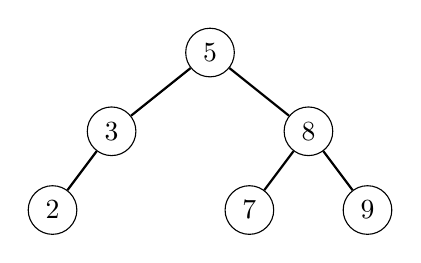
\begin{tikzpicture}[scale=0.5]
\node[draw, circle] (1) at (0,0) {$5$};
\node[draw, circle] (2) at (-2.5,-2) {$3$};
\node[draw, circle] (3) at (2.5,-2) {$8$};
\node[draw, circle] (4) at (-4,-4) {$2$};
\node[draw, circle] (5) at (1,-4) {$7$};
\node[draw, circle] (6) at (4,-4) {$9$};
\path[draw,thick,-] (1) -- (2);
\path[draw,thick,-] (1) -- (3);
\path[draw,thick,-] (2) -- (4);
\path[draw,thick,-] (3) -- (5);
\path[draw,thick,-] (3) -- (6);
\end{tikzpicture}
\caption{Joukkoa $\{2,3,5,7,8,9\}$ vastaava binäärihakupuu.}
\label{fig:bihpuu}
\end{figure}

Kuvassa \ref{fig:bihpuu} on esimerkkinä
joukkoa $\{2,3,5,7,8,9\}$ vastaava binääri\-hakupuu,
jonka juurena on alkio 5.
Vasemmassa alipuussa on kaikki alkiota 5
pienemmät alkiot, eli se vastaa joukkoa $\{2,3\}$.
Oikeassa alipuussa taas on kaikki alkiota 5
suuremmat alkiot, eli se vastaa joukkoa $\{7,8,9\}$.
Huomaa, että tämä on yksi monista tavoista muodostaa
binäärihakupuu kyseiselle joukolle ja voisimme valita myös
minkä tahansa muun alkion puun juureksi.

\subsection{Operaatioiden toteutus}

Seuraavaksi käymme läpi, kuinka voimme toteuttaa
binäärihakupuun avulla operaatioita joukon alkioiden käsittelemiseen.
Osoittautuu, että voimme toteuttaa kaikki
operaatiot ajassa $O(h)$, missä $h$ on puun korkeus.

\subsubsection{Alkion etsiminen}

Kun haluamme etsiä joukosta alkiota $x$, lähdemme liikkeelle
puun juuresta ja kuljemme alaspäin puussa.
Kun olemme solmussa, jossa on alkio $a$,
vaihtoehtoja on kolme.
Jos $a=x$, olemme löytäneet halutun alkion,
jos $a>x$, jatkamme hakua solmun vasempaan lapseen,
ja jos $a<x$, jatkamme hakua solmun oikeaan lapseen.
Jos kuitenkaan solmulla ei ole lasta,
johon meidän tulisi edetä, toteamme,
ettei joukossa ole alkiota $x$.

\begin{figure}
\center
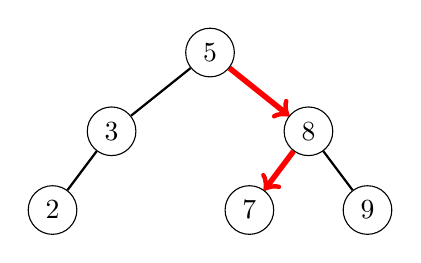
\begin{tikzpicture}[scale=0.5]
\node[draw, circle] (1) at (0,0) {$5$};
\node[draw, circle] (2) at (-2.5,-2) {$3$};
\node[draw, circle] (3) at (2.5,-2) {$8$};
\node[draw, circle] (4) at (-4,-4) {$2$};
\node[draw, circle] (5) at (1,-4) {$7$};
\node[draw, circle] (6) at (4,-4) {$9$};
\path[draw,thick,-] (1) -- (2);
\path[draw,thick,-] (1) -- (3);
\path[draw,thick,-] (2) -- (4);
\path[draw,thick,-] (3) -- (5);
\path[draw,thick,-] (3) -- (6);
\path[draw,thick,red,line width=2pt,->] (1) -- (3);
\path[draw,thick,red,line width=2pt,->] (3) -- (5);
\end{tikzpicture}
\caption{Alkion $7$ etsiminen joukosta $\{2,3,5,7,8,9\}$ juuresta alkaen.}
\label{fig:bihets}
\end{figure}

Kuva \ref{fig:bihets} näyttää, kuinka löydämme alkion 7
joukosta $\{2,3,5,7,8,9\}$.
Juurena on alkio 5, joten alkion 7 täytyy olla juuren
oikeassa alipuussa.
Tämän alipuun juurena on alkio 8,
joten nyt taas tiedämme, että alkion 7 täytyy olla
vasemmassa alipuussa, josta se löytyykin.

\subsubsection{Alkion lisääminen}

Kun haluamme lisätä joukkoon alkion $x$,
jota ei vielä ole joukossa, kuljemme ensin
puussa aivan kuin etsisimme alkiota $x$.
Sitten kun olemme päässeet solmuun,
jolla ei ole lasta, johon meidän tulisi edetä,
luomme uuden solmun alkiolle $x$ ja lisäämme
sen tähän kohtaan lapseksi.

\begin{figure}
\center
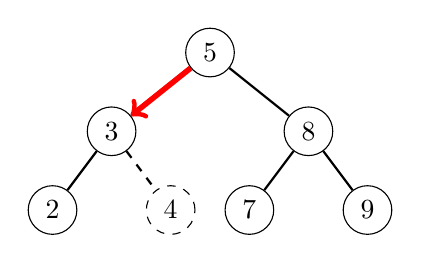
\begin{tikzpicture}[scale=0.5]
\node[draw, circle] (1) at (0,0) {$5$};
\node[draw, circle] (2) at (-2.5,-2) {$3$};
\node[draw, circle] (3) at (2.5,-2) {$8$};
\node[draw, circle] (4) at (-4,-4) {$2$};
\node[draw, circle] (5) at (1,-4) {$7$};
\node[draw, circle] (6) at (4,-4) {$9$};
\node[draw, circle, dashed] (7) at (-1,-4) {$4$};
\path[draw,thick,-] (1) -- (2);
\path[draw,thick,-] (1) -- (3);
\path[draw,thick,-] (2) -- (4);
\path[draw,thick,-] (3) -- (5);
\path[draw,thick,-] (3) -- (6);
\path[draw,thick,dashed,-] (2) -- (7);
\path[draw,thick,red,line width=2pt,->] (1) -- (2);
\end{tikzpicture}
\caption{Alkion 4 lisääminen joukkoon $\{2,3,5,7,8,9\}$.}
\label{fig:bihpu2}
\end{figure}

Kuva \ref{fig:bihpu2} näyttää, kuinka lisäämme alkion 4
joukkoon $\{2,3,5,7,8,9\}$.
Kun haemme puusta alkiota 4, päädymme solmuun,
jossa on alkio 3 ja jolla ei ole oikeaa lasta.
Niinpä luomme alkiolle 4 uuden solmun, jonka asetamme
alkion 3 solmun oikeaksi lapseksi.

\subsubsection{Pienin alkio / suurin alkio}

Kun haluamme löytää joukon pienimmän alkion,
lähdemme liikkeelle juuresta ja etenemme joka askeleella
solmun vasempaan lapseen.
Kun solmulla ei ole enää vasenta lasta,
olemme löytäneet joukon pienimmän alkion.

Vastaavalla tavalla löydämme joukon suurimman alkion
etenemällä koko ajan oikeaan lapseen juuresta.

\subsubsection{Seuraava suurempi alkio / edellinen pienempi alkio}

Kun haluamme löytää joukon pienimmän alkion,
joka on suurempi kuin $x$,
lähdemme liikkeelle puun juuresta.
Kun olemme solmussa, jossa on alkio $a$,
etenemme vasempaan lapseen,
jos $a>x$, ja oikeaan lapseen, jos $a \le x$.
Jatkamme näin, kunnes emme voi edetä alemmas.
Haluttu alkio on pienin alkiota $x$ suurempi alkio
kaikista alkioista, joiden kautta kuljimme.

Kun haluamme vastaavasti löytää joukon suurimman alkion,
joka on pienempi kuin $x$,
menettelemme käänteisesti edelliseen nähden.

\subsubsection{Alkion poistaminen}

Kun haluamme poistaa joukosta alkion $x$, etsimme ensin
alkiota $x$ vastaavan solmun tavalliseen tapaan.
Jos solmulla ei ole lapsia tai vain yksi lapsi,
meidän on helppoa poistaa solmu puusta ja säilyttää
puun rakenne muuten ennallaan.
Jos kuitenkin solmulla on kaksi lasta,
tilanne on hankalampi.
Tällöin etsimme alkion $y$,
joka on pienin $x$:ää suurempi alkio,
ja vaihdamme keskenään alkiot $x$ ja $y$ puussa.
Tämän jälkeen meidän on helppoa poistaa solmu,
jossa on nyt alkio $x$,
koska sillä ei voi olla kahta lasta
(jos solmulla olisi vasen lapsi,
$y$ ei olisi pienin $x$:ää suurempi alkio).

\begin{figure}
\center
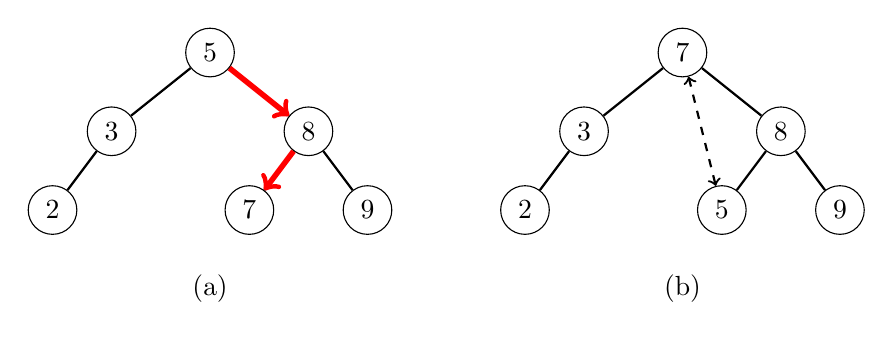
\begin{tikzpicture}[scale=0.5]
\begin{scope}
\node[draw, circle] (1) at (0,0) {$5$};
\node[draw, circle] (2) at (-2.5,-2) {$3$};
\node[draw, circle] (3) at (2.5,-2) {$8$};
\node[draw, circle] (4) at (-4,-4) {$2$};
\node[draw, circle] (5) at (1,-4) {$7$};
\node[draw, circle] (6) at (4,-4) {$9$};
\path[draw,thick,-] (1) -- (2);
\path[draw,thick,-] (1) -- (3);
\path[draw,thick,-] (2) -- (4);
\path[draw,thick,-] (3) -- (5);
\path[draw,thick,-] (3) -- (6);
\path[draw,thick,red,line width=2pt,->] (1) -- (3);
\path[draw,thick,red,line width=2pt,->] (3) -- (5);
\node at (0,-6) {(a)};
\end{scope}
\begin{scope}[xshift=12cm]
\node[draw, circle] (1) at (0,0) {$7$};
\node[draw, circle] (2) at (-2.5,-2) {$3$};
\node[draw, circle] (3) at (2.5,-2) {$8$};
\node[draw, circle] (4) at (-4,-4) {$2$};
\node[draw, circle] (5) at (1,-4) {$5$};
\node[draw, circle] (6) at (4,-4) {$9$};
\path[draw,thick,-] (1) -- (2);
\path[draw,thick,-] (1) -- (3);
\path[draw,thick,-] (2) -- (4);
\path[draw,thick,-] (3) -- (5);
\path[draw,thick,-] (3) -- (6);
\path[draw,thick,<->,dashed] (1) -- (5);
\node at (0,-6) {(b)};
\end{scope}
\end{tikzpicture}
\caption{Alkion 5 poistaminen joukosta $\{2,3,5,7,8,9\}$. (a) Koska alkiolla
5 on kaksi lasta, etsimme seuraavan suuremman alkion 7.
(b) Vaihdamme keskenään alkiot 5 ja 7, minkä jälkeen voimme poistaa helposti alkion 5.}
\label{fig:bihpu3}
\end{figure}

Kuva \ref{fig:bihpu3} näyttää, kuinka poistamme joukosta $\{2,3,5,7,8,9\}$ alkion 5.
Alkio on puun juuressa ja solmulla on kaksi lasta,
joten meidän tulee etsiä ensin pienin alkiota 5 suurempi alkio,
joka on 7.
Vaihdamme sitten keskenään arvot 5 ja 7,
minkä jälkeen meidän on helppoa poistaa alkio 5.

\subsection{Operaatioiden tehokkuus}

Binäärihakupuun operaatiot vievät aikaa $O(h)$,
missä $h$ on puun korkeus, joten operaatioiden tehokkuus
riippuu puun korkeudesta.
Operaatioiden tehokkuuteen vaikuttaa siis,
miten olemme rakentaneet puun.
Esimerkiksi kuvassa \ref{fig:bihkor} on kaksi mahdollista
binäärihakupuuta joukolle $\{1,2,3,4,5\}$.
Vasemman puun korkeus on 2, kun taas oikean puun korkeus on 4.

\begin{figure}
\center
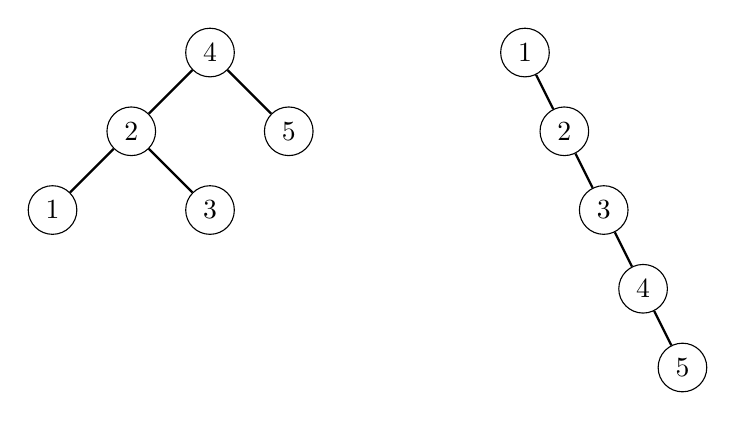
\begin{tikzpicture}[scale=0.5]
\begin{scope}
\node[draw, circle] (1) at (0,0) {$1$};
\node[draw, circle] (2) at (1,-2) {$2$};
\node[draw, circle] (3) at (2,-4) {$3$};
\node[draw, circle] (4) at (3,-6) {$4$};
\node[draw, circle] (5) at (4,-8) {$5$};
\path[draw,thick,-] (1) -- (2);
\path[draw,thick,-] (2) -- (3);
\path[draw,thick,-] (3) -- (4);
\path[draw,thick,-] (4) -- (5);
\end{scope}
\begin{scope}[xshift=-8cm]
\node[draw, circle] (1) at (0,0) {$4$};
\node[draw, circle] (2) at (-2,-2) {$2$};
\node[draw, circle] (3) at (2,-2) {$5$};
\node[draw, circle] (4) at (-4,-4) {$1$};
\node[draw, circle] (5) at (0,-4) {$3$};
\path[draw,thick,-] (1) -- (2);
\path[draw,thick,-] (1) -- (3);
\path[draw,thick,-] (2) -- (4);
\path[draw,thick,-] (2) -- (5);
\end{scope}
\end{tikzpicture}
\caption{Kaksi binäärihakupuuta joukolle $\{1,2,3,4,5\}$.
Vasemman puun korkeus on 2 ja oikean puun korkeus on 4.}
\label{fig:bihkor}
\end{figure}

\index{tasapainoinen puu}

Jotta binäärihakupuu toimisi tehokkaasti, haluamme,
että puun korkeus ei kasva liian suureksi.
Tarkemmin ottaen tavoitteemme on, että
solmut ovat jakautuneet tasaisesti puun eri puolille
ja puun korkeus on $O(\log n)$.
Tällöin sanomme, että puu on \emph{tasapainoinen} (\emph{balanced}).
Jos onnistumme tässä, kaikki puun operaatiot toimivat
tehokkaasti ajassa $O(\log n)$.
Saavutamme tavoitteemme
lisäämällä puuhun ehtoja, jotka rajoittavat
sen korkeutta sopivasti.

Binäärihakupuun tasapainottamiseen tunnetaan monia menetelmiä.
Tutustumme seuraavaksi AVL-puuhun, joka on 
varhaisin tunnettu tasapainoinen binäärihakupuu.
AVL-puu on yksinkertaisempi kuin monet myöhemmin
kehitetyt rakenteet, minkä vuoksi se sopii hyvin esittelemään
puiden tasapainotuksen ideoita.
Javan ja muiden ohjelmointikielten standardikirjastoissa
käyte\-tään kuitenkin muita rakenteita, kuten punamustaa puuta.

\section{AVL-puu}

\index{AVL-puu}

\emph{AVL-puu} (\emph{AVL tree}) on tasapainoinen binäärihakupuu, jonka
korkeus on aina $O(\log n)$, minkä ansiosta puun operaatiot
toimivat tehokkaasti ajassa $O(\log n)$.
AVL-puussa jokaiseen solmuun liittyy \emph{tasapainoehto},
joka takaa, että puu on tasapainoinen.
Kun päivitämme puuta, meidän täytyy pitää huolta siitä,
että tasapainoehto säilyy voimassa kaikissa solmuissa.

\subsection{Tasapainoehto}

AVL-puun tasapainoehtona on, että
\emph{jokaisessa solmussa vasemman ja oikean lapsen
alipuiden korkeusero on enintään 1}.

Esimerkiksi kuvan \ref{fig:bihkor} vasen puu on
AVL-puu, kun taas oikea puu ei ole.
Oikea puu ei ole AVL-puu, koska esimerkiksi solmussa 1
vasemman lapsen alipuun korkeus on $-1$ mutta oikean lapsen
alipuun korkeus on 3.
Korkeuksien erona on siis 4, vaikka ero saisi olla enintään 1.

\index{AVL-ehto}

Kutsumme AVL-puun tasapainoehtoa \emph{AVL-ehdoksi}.
Osoittautuu, että jos binäärihakupuu täyttää AVL-ehdon,
sen korkeus on $O(\log n)$.
Eli jos pystymme toteuttamaan puun operaatiot niin,
että AVL-ehto säilyy, saamme aikaan binäärihakupuun,
jonka operaatiot toimivat ajassa $O(\log n)$.

\begin{figure}
\center
\scriptsize
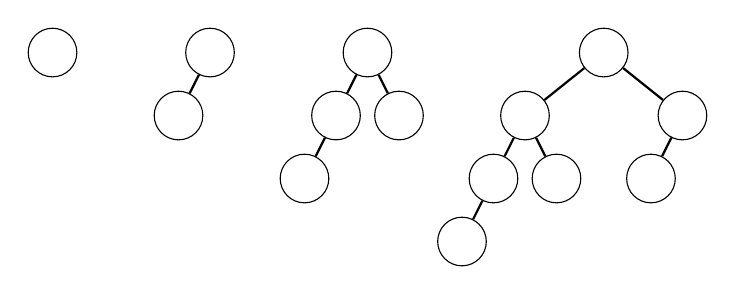
\begin{tikzpicture}[scale=0.4]
\begin{scope}
\node[draw, circle] (2) at (-2.5,-2) {\phantom{$1$}};
\end{scope}
\begin{scope}[xshift=5cm]
\node[draw, circle] (2) at (-2.5,-2) {\phantom{$1$}};
\node[draw, circle] (4) at (-3.5,-4) {\phantom{$1$}};
\path[draw,thick,-] (2) -- (4);
\end{scope}
\begin{scope}[xshift=10cm]
\node[draw, circle] (2) at (-2.5,-2) {\phantom{$1$}};
\node[draw, circle] (4) at (-3.5,-4) {\phantom{$1$}};
\node[draw, circle] (5) at (-1.5,-4) {\phantom{$1$}};
\node[draw, circle] (7) at (-4.5,-6) {\phantom{$1$}};
\path[draw,thick,-] (2) -- (4);
\path[draw,thick,-] (2) -- (5);
\path[draw,thick,-] (4) -- (7);
\end{scope}
\begin{scope}[xshift=15cm,yshift=-2cm]
\node[draw, circle] (1) at (0,0) {\phantom{$1$}};
\node[draw, circle] (2) at (-2.5,-2) {\phantom{$1$}};
\node[draw, circle] (3) at (2.5,-2) {\phantom{$1$}};
\node[draw, circle] (4) at (-3.5,-4) {\phantom{$1$}};
\node[draw, circle] (5) at (-1.5,-4) {\phantom{$1$}};
\node[draw, circle] (6) at (1.5,-4) {\phantom{$1$}};
\node[draw, circle] (7) at (-4.5,-6) {\phantom{$1$}};
\path[draw,thick,-] (1) -- (2);
\path[draw,thick,-] (1) -- (3);
\path[draw,thick,-] (2) -- (4);
\path[draw,thick,-] (2) -- (5);
\path[draw,thick,-] (3) -- (6);
\path[draw,thick,-] (4) -- (7);
\end{scope}
\end{tikzpicture}
\caption{Vähiten solmuja sisältävät AVL-puut korkeuksille 0, 1, 2 ja 3.}
\label{fig:avlvah}
\end{figure}

Miksi sitten AVL-ehto takaa, että binäärihakupuun korkeus
on $O(\log n)$?
Voimme lähestyä asiaa pahimman tapauksen kautta:
kun tiedämme, että AVL-puussa on $n$ solmua,
mikä on sen \emph{suurin mahdollinen} korkeus?
Voimme selvittää tämän laskemalla ensin käänteisesti,
mikä on \emph{pienin mahdollinen} solmujen määrä
AVL-puussa, jonka korkeus on $h$.

Merkitään $f(h)$:lla korkeutta $h$ olevan AVL-puun
pienintä mahdollista solmujen määrää.
Kuvan \ref{fig:avlvah} mukaisesti funktion ensimmäiset arvot
ovat $f(0)=1$, $f(1)=2$, $f(2)=4$ ja $f(3)=7$.
Yleisemmin
\[f(h)=1+f(h-1)+f(h-2),\]
kun $h \ge 2$, koska jos haluamme rakentaa AVL-puun korkeutta $h$,
jossa on mahdollisimman vähän solmuja,
meidän kannattaa laittaa juuren lapsiksi AVL-puut
korkeutta $h-1$ ja $h-2$ niin,
että kummassakin alipuussa on mahdollisimman vähän solmuja.
Funktiolle pätee
\[f(h) \ge 2 f(h-2),\]
eli funktion arvo ainakin kaksinkertaistuu kahden askeleen välein.
Voimme ilmaista tämän alarajan
\[f(h) \ge 2^{h/2},\]
jonka voimme taas muuttaa ylärajaksi
\[ h \le 2 \log f(h).\]

Tarkastellaan sitten puuta, jossa on $n$ solmua
ja jonka korkeus on $h$.
Korkeudelle täytyy päteä $f(h) \le n$,
koska korkeutta $h$ olevassa puussa on vähintään $f(h)$ solmua.
Niinpä saamme ylärajan
\[h \le 2 \log n,\]
mikä tarkoittaa samaa kuin $h = O(\log n)$.

\subsection{Kiertojen toteuttaminen}

\begin{figure}
\center
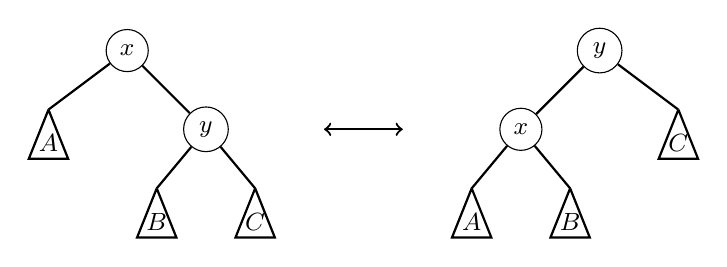
\begin{tikzpicture}[scale=0.5]
\small
\newcommand\alipuu[3]{
\path[draw,thick,-] (0+#1,0+#2) -- (-0.5+#1,-1.25+#2) -- (0.5+#1,-1.25+#2) -- (0+#1,0+#2);
\node at (0+#1,-0.85+#2) {#3};
}
\draw[thick,<->] (5,-2) -- (7,-2);
\begin{scope}
\node[draw, circle] (1) at (0,0) {$x$};
\node[draw, circle] (2) at (2,-2) {$y$};
\alipuu{-2}{-1.5}{$A$}
\alipuu{0.75}{-3.5}{$B$}
\alipuu{3.25}{-3.5}{$C$}
\path[draw,thick,-] (1) -- (2);
\path[draw,thick,-] (1) -- (-2,-1.5);
\path[draw,thick,-] (2) -- (0.75,-3.5);
\path[draw,thick,-] (2) -- (3.25,-3.5);
\end{scope}
\begin{scope}[xshift=10cm]
\node[draw, circle] (1) at (0,-2) {$x$};
\node[draw, circle] (2) at (2,0) {$y$};
\alipuu{-1.25}{-3.5}{$A$}
\alipuu{1.25}{-3.5}{$B$}
\alipuu{4}{-1.5}{$C$}
\path[draw,thick,-] (1) -- (2);
\path[draw,thick,-] (1) -- (-1.25,-3.5);
\path[draw,thick,-] (1) -- (1.25,-3.5);
\path[draw,thick,-] (2) -- (4,-1.5);
\end{scope}
\end{tikzpicture}
\caption{Kierrot, joiden avulla korjaamme AVL-puuta.}
\label{fig:avlkie}
\end{figure}

\index{kierto}

Voimme toteuttaa AVL-puun operaatiot muuten samaan tapaan
kuin yleisessä binäärihakupuussa, mutta meidän täytyy varmistaa
alkion lisäämisen ja poistamisen jälkeen, että AVL-ehto
on edelleen voimassa.
Tämä onnistuu tekemällä sopivia \emph{kiertoja} (\emph{rotation}),
jotka muuttavat puun rakennetta.
Jotta voimme toteuttaa kierrot, pidämme jokaisessa
solmussa tietoa siitä, mikä on solmusta alkavan alipuun korkeus.

Osoittautuu, että voimme korjata puun rakenteen kaikissa
tilanteessa käyttäen kahta kiertotyyppiä,
jotka on esitetty kuvassa \ref{fig:avlkie}.
Kierrämme solmuja $x$ ja $y$,
joihin liittyvät alipuut $A$, $B$ ja $C$.
Voimme tehdä kierron joko vasemmalta oikealle,
jolloin solmu $y$ nousee ylöspäin,
tai oikealta vasemmalle,
jolloin solmu $x$ nousee ylöspäin.

\begin{figure}
\center
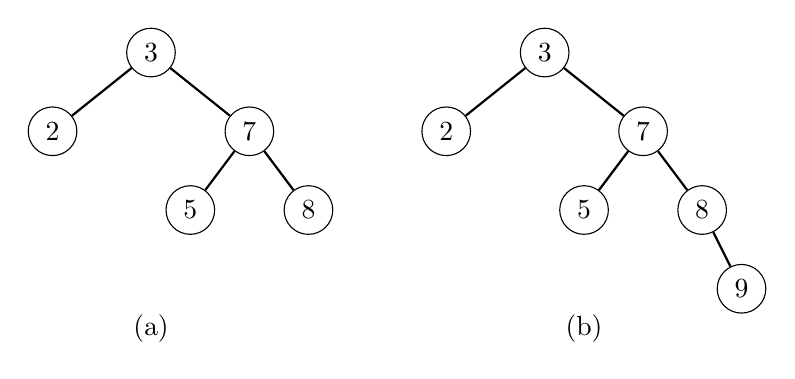
\begin{tikzpicture}[scale=0.5]
\begin{scope}
\node[draw, circle] (1) at (0,0) {$3$};
\node[draw, circle] (2) at (-2.5,-2) {$2$};
\node[draw, circle] (3) at (2.5,-2) {$7$};
\node[draw, circle] (5) at (1,-4) {$5$};
\node[draw, circle] (6) at (4,-4) {$8$};
\path[draw,thick,-] (1) -- (2);
\path[draw,thick,-] (1) -- (3);
\path[draw,thick,-] (3) -- (5);
\path[draw,thick,-] (3) -- (6);
\node at (0,-7) {(a)};
\end{scope}
\begin{scope}[xshift=10cm]
\node[draw, circle] (1) at (0,0) {$3$};
\node[draw, circle] (2) at (-2.5,-2) {$2$};
\node[draw, circle] (3) at (2.5,-2) {$7$};
\node[draw, circle] (5) at (1,-4) {$5$};
\node[draw, circle] (6) at (4,-4) {$8$};
\node[draw, circle] (7) at (5,-6) {$9$};
\path[draw,thick,-] (1) -- (2);
\path[draw,thick,-] (1) -- (3);
\path[draw,thick,-] (3) -- (5);
\path[draw,thick,-] (3) -- (6);
\path[draw,thick,-] (6) -- (7);
\node at (1,-7) {(b)};
\end{scope}
\end{tikzpicture}
\caption{(a) Jokaisessa puun solmussa pätee AVL-ehto.
(b) AVL-ehto menee rikki solmussa 3, kun lisäämme puuhun solmun 9.}
\label{fig:avlrik}
\end{figure}

Kun lisäämme AVL-puuhun solmun, jonkin solmun AVL-ehto
voi rikkoontua. Tämä ilmenee niin,
että jossain solmussa lasten alipuiden korkeudet ovat ennen lisäämistä
$h$ ja $h+1$ ja lisäämisen jälkeen $h$ ja $h+2$.
Kuva \ref{fig:avlrik} näyttää esimerkin tällaisesta tilanteesta.
Vasemmassa puussa solmun $3$ lasten korkeudet ovat 0 ja 1,
joten AVL-ehto on kunnossa.
Oikeassa puussa olemme lisänneet solmun $9$,
minkä seurauksena solmun $3$ lasten korkeudet ovat 0 ja 2
eikä AVL-ehto enää päde.

\begin{figure}
\center
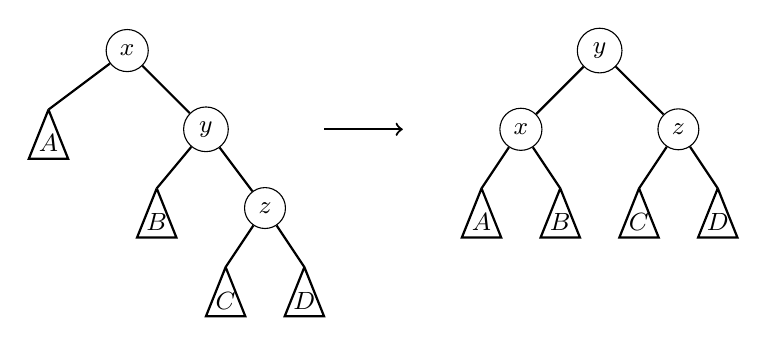
\begin{tikzpicture}[scale=0.5]
\small
\newcommand\alipuu[3]{
\path[draw,thick,-] (0+#1,0+#2) -- (-0.5+#1,-1.25+#2) -- (0.5+#1,-1.25+#2) -- (0+#1,0+#2);
\node at (0+#1,-0.85+#2) {#3};
}
\draw[thick,->] (5,-2) -- (7,-2);
\begin{scope}
\node[draw, circle] (1) at (0,0) {$x$};
\node[draw, circle] (2) at (2,-2) {$y$};
\node[draw, circle] (3) at (3.5,-4) {$z$};
\alipuu{-2}{-1.5}{$A$}
\alipuu{0.75}{-3.5}{$B$}
\alipuu{2.5}{-5.5}{$C$}
\alipuu{4.5}{-5.5}{$D$}
\path[draw,thick,-] (1) -- (2);
\path[draw,thick,-] (2) -- (3);
\path[draw,thick,-] (1) -- (-2,-1.5);
\path[draw,thick,-] (2) -- (0.75,-3.5);
\path[draw,thick,-] (3) -- (2.5,-5.5);
\path[draw,thick,-] (3) -- (4.5,-5.5);
\end{scope}
\begin{scope}[xshift=12cm]
\node[draw, circle] (1) at (-2,-2) {$x$};
\node[draw, circle] (2) at (0,0) {$y$};
\node[draw, circle] (3) at (2,-2) {$z$};
\alipuu{-3}{-3.5}{$A$}
\alipuu{-1}{-3.5}{$B$}
\alipuu{1}{-3.5}{$C$}
\alipuu{3}{-3.5}{$D$}
\path[draw,thick,-] (1) -- (2);
\path[draw,thick,-] (2) -- (3);
\path[draw,thick,-] (1) -- (-3,-3.5);
\path[draw,thick,-] (1) -- (-1,-3.5);
\path[draw,thick,-] (3) -- (1,-3.5);
\path[draw,thick,-] (3) -- (3,-3.5);
\end{scope}
\end{tikzpicture}
\caption{Tapaus 1: nostamme solmua $y$ ylöspäin.}
\label{fig:avlta1}
\end{figure}

\begin{figure}
\center
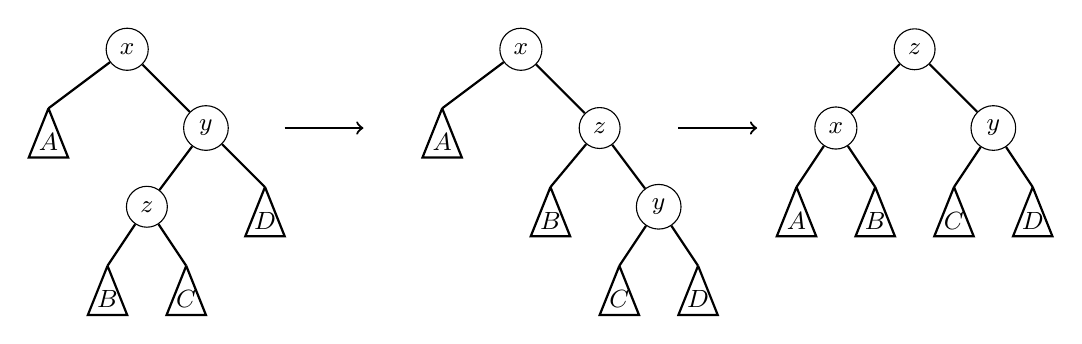
\begin{tikzpicture}[scale=0.5]
\small
\newcommand\alipuu[3]{
\path[draw,thick,-] (0+#1,0+#2) -- (-0.5+#1,-1.25+#2) -- (0.5+#1,-1.25+#2) -- (0+#1,0+#2);
\node at (0+#1,-0.85+#2) {#3};
}
\draw[thick,->] (4,-2) -- (6,-2);
\draw[thick,->] (14,-2) -- (16,-2);
\begin{scope}
\node[draw, circle] (1) at (0,0) {$x$};
\node[draw, circle] (2) at (2,-2) {$y$};
\node[draw, circle] (3) at (0.5,-4) {$z$};
\alipuu{-2}{-1.5}{$A$}
\alipuu{-0.5}{-5.5}{$B$}
\alipuu{1.5}{-5.5}{$C$}
\alipuu{3.5}{-3.5}{$D$}
\path[draw,thick,-] (1) -- (2);
\path[draw,thick,-] (2) -- (3);
\path[draw,thick,-] (1) -- (-2,-1.5);
\path[draw,thick,-] (3) -- (-0.5,-5.5);
\path[draw,thick,-] (3) -- (1.5,-5.5);
\path[draw,thick,-] (2) -- (3.5,-3.5);
\end{scope}
\begin{scope}[xshift=10cm]
\node[draw, circle] (1) at (0,0) {$x$};
\node[draw, circle] (2) at (2,-2) {$z$};
\node[draw, circle] (3) at (3.5,-4) {$y$};
\alipuu{-2}{-1.5}{$A$}
\alipuu{0.75}{-3.5}{$B$}
\alipuu{2.5}{-5.5}{$C$}
\alipuu{4.5}{-5.5}{$D$}
\path[draw,thick,-] (1) -- (2);
\path[draw,thick,-] (2) -- (3);
\path[draw,thick,-] (1) -- (-2,-1.5);
\path[draw,thick,-] (2) -- (0.75,-3.5);
\path[draw,thick,-] (3) -- (2.5,-5.5);
\path[draw,thick,-] (3) -- (4.5,-5.5);
\end{scope}
\begin{scope}[xshift=20cm]
\node[draw, circle] (1) at (-2,-2) {$x$};
\node[draw, circle] (2) at (0,0) {$z$};
\node[draw, circle] (3) at (2,-2) {$y$};
\alipuu{-3}{-3.5}{$A$}
\alipuu{-1}{-3.5}{$B$}
\alipuu{1}{-3.5}{$C$}
\alipuu{3}{-3.5}{$D$}
\path[draw,thick,-] (1) -- (2);
\path[draw,thick,-] (2) -- (3);
\path[draw,thick,-] (1) -- (-3,-3.5);
\path[draw,thick,-] (1) -- (-1,-3.5);
\path[draw,thick,-] (3) -- (1,-3.5);
\path[draw,thick,-] (3) -- (3,-3.5);
\end{scope}
\end{tikzpicture}
\caption{Tapaus 2: nostamme solmua $z$ kahdesti ylöspäin.}
\label{fig:avlta2}
\end{figure}

Solmun lisäämisen jälkeen kuljemme puussa ylöspäin
lisätystä solmusta juureen ja päivitämme solmujen korkeudet.
Jos jokin solmu ei täytä AVL-ehtoa, korjaamme asian tekemällä yhden
tai kaksi kiertoa.
Oletetaan, että $x$ on alimpana puussa oleva solmu, jossa AVL-ehto ei päde,
$y$ on $x$:n lapsi, jonka alipuussa on lisätty solmu,
ja $z$ on puolestaan $y$:n lapsi, jonka alipuussa on lisätty solmu.
Tapauksia on kaksi: jos $y$ ja $z$ ovat samanpuoleisia lapsia,
kierrämme solmua $y$ kerran ylöspäin (kuva \ref{fig:avlta1}),
ja muuten kierrämme solmua $z$ kahdesti ylöspäin (kuva \ref{fig:avlta2}).
Tämän korjauksen jälkeen AVL-ehto on jälleen
voimassa kaikissa puun solmuissa, eli meidän riittää aina
korjata ehto alimmassa solmussa, jossa se ei ole voimassa.

Kuvassa \ref{fig:avlrik}(b) AVL-ehto ei ole voimassa solmussa $3$,
koska vasemman alipuun korkeus on 0 ja oikean alipuun korkeus on 2.
Tässä tapauksessa $x=3$, $y=7$ ja $z=8$.
Koska $y$ on $x$:n oikea lapsi ja $z$ on $y$:n oikea lapsi,
meidän riittää tehdä yksi kierto, joka nostaa solmua $7$ ylöspäin
puun juureksi.
Tuloksena on kuvan \ref{fig:avlkor} mukainen puu, jossa
AVL-ehto on jälleen voimassa,
koska solmun $7$ kummankin alipuun korkeus on nyt 1.

\begin{figure}
\center
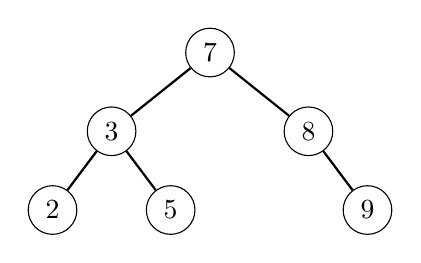
\begin{tikzpicture}[scale=0.5]
\node[draw, circle] (1) at (0,0) {$7$};
\node[draw, circle] (2) at (-2.5,-2) {$3$};
\node[draw, circle] (3) at (2.5,-2) {$8$};
\node[draw, circle] (5) at (-4,-4) {$2$};
\node[draw, circle] (6) at (-1,-4) {$5$};
\node[draw, circle] (7) at (4,-4) {$9$};
\path[draw,thick,-] (1) -- (2);
\path[draw,thick,-] (1) -- (3);
\path[draw,thick,-] (2) -- (5);
\path[draw,thick,-] (2) -- (6);
\path[draw,thick,-] (3) -- (7);
\end{tikzpicture}
\caption{Kierrämme solmun $7$ puun juureksi, jolloin AVL-ehto pätee taas.}
\label{fig:avlkor}
\end{figure}

Kun poistamme puusta solmun, menettelemme melko samalla tavalla
kuin lisäämisessä.
Nyt on mahdollista, että ennen poistoa
jossakin solmussa lasten alipuiden korkeudet ovat $h$ ja $h-1$
ja poiston jälkeen $h$ ja $h-2$.
Poiston jälkeen nousemme puussa ylöspäin
poistetun solmun vanhemmasta alkaen, ja jos vastaan tulee solmu $x$,
jossa AVL-ehto ei päde, korjaamme asian.
Tällä kertaa valitsemme solmut $y$ ja $z$ niin,
että $y$ on $x$:n lapsi, jonka korkeus on suurin,
ja samoin $z$ on $y$:n lapsi, jonka korkeus on suurin.
Jos $y$:n kummankin lapsen korkeus on sama,
valitsemme $z$:n niin, että se on samanpuoleinen lapsi kuin $y$.
Sitten korjaamme AVL-ehdon kierroilla kuten solmun lisäämisessä.
Toisin kuin lisäämisessä, saatamme joutua korjaamaan ehdon
useassa solmussa,
koska ehdon korjaaminen yhdessä solmussa voi rikkoa
sen jossain ylemmässä solmussa.
Kun lopulta saavumme juureen, AVL-ehto pätee jälleen kaikissa solmuissa.

Koska AVL-puun korkeus on $O(\log n)$ ja jokainen kierto
tapahtuu vakioajassa,
pystymme korjaamaan tasapainon sekä lisäämisen että poistamisen
jälkeen ajassa $O(\log n)$.
Lisäämisen jälkeen kuljemme puuta ylöspäin $O(\log n)$ askelta
ja teemme enintään kaksi kiertoa.
Poistamisen jälkeen taas kuljemme puuta ylöspäin $O(\log n)$ askelta
ja teemme enintään $O(\log n)$ kiertoa.

\section{Javan toteutukset}

Javan tietorakenteet \texttt{TreeSet} ja \texttt{TreeMap}
pohjautuvat punamustaan puuhun,
joka on AVL-puun tapainen mutta monimutkaisempi
binäärihakupuu.
Ne muistuttavat rakenteita \texttt{HashSet} ja \texttt{HashMap},
mutta erona on, että pystymme lisäksi etsimään
alkioita niiden järjestyksen perusteella.
Rakenteiden operaatiot toimivat ajassa $O(\log n)$.

\subsection{\texttt{TreeSet}-rakenne}

Seuraava koodi luo \texttt{TreeSet}-rakenteen,
joka pitää yllä lukujen joukkoa.
Koodi lisää joukkoon alkioita ja tulostaa sitten sen sisällön.
Huomaa, että tulostuksessa joukon alkiot näkyvät
järjestyksessä pienimmästä suurimpaan, koska
binäärihakupuu pitää niitä järjestyksessä.

\begin{code}
TreeSet<Integer> joukko = new TreeSet<>();
joukko.add(4);
joukko.add(1);
joukko.add(8);
joukko.add(7);
System.out.println(joukko); // [1, 4, 7, 8]
\end{code}

Koska joukko on järjestyksessä, pystymme etsimään tehokkaasti
pienim\-män ja suurimman alkion metodeilla \texttt{first} ja \texttt{last}:

\begin{code}
System.out.println(joukko.first()); // 1
System.out.println(joukko.last()); // 8
\end{code}

Pystymme myös etsimään seuraavan tiettyä alkiota
suuremman tai pienemmän alkion metodeilla \texttt{higher} ja \texttt{lower}:

\begin{code}
System.out.println(joukko.higher(5)); // 7
System.out.println(joukko.lower(5)); // 4
\end{code}

\subsection{\texttt{TreeMap}-rakenne}

Seuraava koodi luo sanakirjan \texttt{TreeMap}-rakenteen avulla:

\begin{code}
TreeMap<String,String> sanakirja = new TreeMap<>();
sanakirja.put("apina","monkey");
sanakirja.put("banaani","banana");
sanakirja.put("cembalo","harpsichord");
\end{code}

Tämä sanakirja muodostuu avain-arvo-pareista,
joissa avaimet ovat suomen kielen sanoja
ja arvot ovat englannin kielen sanoja.
Sanakirjan sisältö on järjestetty avaimien perusteella.
Esimerkiksi voimme selvittää, mikä on aakkosjärjestyksessä
ensimmäinen ja viimeinen avain:

\begin{code}
System.out.println(sanakirja.firstKey()); // apina
System.out.println(sanakirja.lastKey()); // cembalo
\end{code}

Samoin voimme selvittää lähinnä tiettyä avainta olevat avaimet:

\begin{code}
System.out.println(sanakirja.higherKey("biisoni")); // cembalo
System.out.println(sanakirja.lowerKey("biisoni")); // banaani
\end{code}

\subsection{Omat luokat}

Jos haluamme käyttää omia olioitamme \texttt{TreeSet}- ja
\texttt{TreeMap}-rakenteissa, meidän tulee toteuttaa
luokkaan kaksi metodia:
\texttt{equals} ilmaisee, ovatko kaksi oliota samat,
ja \texttt{compareTo} kertoo kahden olion suuruusjärjestyksen.
Jälkimmäisen metodin ansiosta luokka toteuttaa rajapinnan
\texttt{Comparable}.

Miksi oikeastaan metodi \texttt{equals} on tarpeen?
Metodi \texttt{compareTo} palauttaa arvon 0 tarkalleen silloin,
kun alkiot ovat yhtä suuret, joten myös sen avulla voi
tarkastaa asian.
Syynä on, että \texttt{TreeSet} toteuttaa rajapinnan \texttt{Set},
joka edellyttää, että luokassa on oikein toimiva metodi \texttt{equals},
vaikka siitä ei sinänsä olekaan hyötyä tässä tapauksessa.

\section{Tehokkuusvertailu}

Monissa ongelmissa meillä on kaksi mahdollista lähestymistapaa:
voimme käyttää joko joukkorakenteita tai sitten taulukoita ja järjestämistä.
Vaikka molemmat tavat johtavat tehokkaaseen ratkaisuun,
vakiokertoimissa voi olla merkittäviä eroja, jotka vaikuttavat
käytännön tehokkuuteen.

Tarkastelemme seuraavaksi ongelmaa, jossa meille on annettu
$n$ lukua sisältävä taulukko, ja haluamme selvittää,
montako eri lukua taulukossa on.
Ratkaisemme ongelman kolmella eri tavalla ja tutkimme sitten
ratkaisujen tehokkuutta.

\subsubsection{Ratkaisu 1: \texttt{TreeSet}}

Ensimmäinen tapa ratkaista tehtävä on luoda \texttt{TreeSet},
johon lisäämme taulukon luvut.
Koska jokainen luku voi esiintyä joukossa vain kerran,
joukon koko ilmaisee meille, montako eri lukua taulukossa on.
Tämä ratkaisu vie aikaa $O(n \log n)$, koska jokainen
\texttt{add}-operaatio vie aikaa $O(\log n)$.

\begin{code}
TreeSet<Integer> joukko = new TreeSet<>();
for (int i = 0; i < taulu.length; i++) {
    joukko.add(taulu[i]);
}
System.out.println(joukko.size());
\end{code}

\subsubsection{Ratkaisu 2: \texttt{HashSet}}

Emme tarvitse \texttt{TreeSet}-rakenteen
alkioiden järjestystä, joten saamme toisen ratkaisun
käyttämällä sen sijaan \texttt{HashSet}-rakennetta.
Koodi säilyy muuten täysin samanlaisena.
Tämä ratkaisu vie aikaa $O(n)$ hajautuksen ansiosta.

\begin{code}
HashSet<Integer> joukko = new HashSet<>();
for (int i = 0; i < taulu.length; i++) {
    joukko.add(taulu[i]);
}
System.out.println(joukko.size());
\end{code}

\subsubsection{Ratkaisu 3: järjestäminen}

Kolmas tapa ratkaista tehtävä on käyttää järjestämistä:
kopioimme ensin luvut uuteen taulukkoon, järjestämme tämän taulukon ja
tutkimme sitten, monessako kohdassa järjestetyssä taulukossa luku vaihtuu.
Tämä ratkaisu vie aikaa $O(n \log n)$, koska taulukon järjestäminen
vie aikaa $O(n \log n)$.

\begin{code}
int[] kopio = taulu.clone();
Arrays.sort(kopio);
int laskuri = 1;
for (int i = 1; i < kopio.length; i++) {
    if (kopio[i-1] != kopio[i]) laskuri++;
}
System.out.println(laskuri);
\end{code}

\subsubsection{Vertailun tulokset}

Taulukko \ref{tab:eriver} esittää tehokkuusvertailun tulokset.
Jokaisessa testissä taulukossa on satunnaisia lukuja väliltä $1 \dots 10^9$.

Osoittautuu, että ratkaisujen välillä on merkittäviä tehokkuuseroja.
Ensinnäkin \texttt{HashSet}-ratkaisu on noin kolme kertaa
nopeampi kuin \texttt{TreeSet}-ratkaisu.
Tämä onkin odotettavaa, koska hajautustaulun
operaatiot vievät aikaa $O(1)$, kun taas binäärihakupuun
operaatiot vievät aikaa $O(\log n)$.
Selvästi nopein ratkaisu on kuitenkin kolmas järjestämistä
käyttävä ratkaisu, joka on noin kymmenen kertaa
\texttt{TreeSet}-ratkaisua nopeampi.

Miten on mahdollista, että sekä \texttt{TreeSet}-ratkaisun että
järjestämisrat\-kaisun aikavaativuus on $O(n \log n)$, mutta
järjestämisratkaisu on kymmenen kertaa nopeampi?
Tämä johtuu siitä, että taulukon järjestäminen on hyvin kevyt
operaatio ja se tehdään vain kerran.
Binäärihakupuussa jokainen lisäys muuttaa puun rakennetta,
mikä aiheuttaa suuret vakiokertoimet.

Vaikka joukot ovat käteviä, niitä ei siis kannata
käyttää turhaan.
Jos haluamme ratkaista ongelman todella tehokkaasti,
kannattaa miettiä, voisimmeko käyttää tavalla tai toisella
järjestämistä joukkojen sijaan.

\begin{table}
\center
\begin{tabular}{rrrr}
taulukon koko $n$ & \texttt{TreeSet} & \texttt{HashSet} & järjestäminen \\
\hline
$10^6$ & 0.74 s & 0.25 s & 0.09 s \\
$2 \cdot 10^6$ & 1.60 s & 0.45 s & 0.19 s \\
$4 \cdot 10^6$ & 5.60 s & 1.56 s & 0.52 s \\
$8 \cdot 10^6$ & 12.19 s & 4.50 s & 0.97 s \\
\end{tabular}
\caption{Algoritmien suoritusaikojen vertailu.}
\label{tab:eriver}
\end{table}

\chapter{Binäärihakupuu}

Binäärihakupuu on tietorakenne, joka pitää yllä alkioiden joukkoa.
Binääri\-hakupuun perusoperaatiot ovat samat kuin hajautustaulussa:

\begin{itemize}
\item lisää alkio $x$ joukkoon
\item tarkista, onko alkio $x$ joukossa
\item poista alkio $x$ joukosta
\end{itemize}

Koska binäärihakupuu säilyttää joukon alkioita
\emph{järjestyksessä}, voimme toteuttaa lisäksi tehokkaasti
esimerkiksi seuraavat operaatiot:

\begin{itemize}
\item etsi joukon pienin/suurin alkio
\item etsi joukon pienin alkio, joka on vähintään $x$
\item etsi joukon suurin alkio, joka on enintään $x$
\end{itemize}

Hajautustaulu \emph{ei} pysty tarjoamaan tällaisia operaatioita
tehokkaasti, joten binäärihakupuu on hyvä valinta, jos näille
operaatioille on tarvetta joukon perusoperaatioiden lisäksi.

Voimme toteuttaa binäärihakupuun niin,
että kaikki sen operaatiot toimivat ajassa $O(\log n)$.
Tämä vaatii, että puu on \emph{tasapainoinen},
minkä saavuttamiseksi on monia menetelmiä.
Tässä luvussa tutustumme AVL-puuhun, joka on
yksinkertainen esimerkki tasapainoisesta binääripuusta.
Javan tietorakenteet perustuvat taas punamustaan puuhun,
joka on AVL-puuta vaikeampi toteuttaa mutta tietyissä tilanteissa tehokkaampi.

\section{Taustaa binääripuista}

Binäärihakupuun taustalla on yleisempi tietorakenne \emph{binääripuu}.
Ennen kuin tutustumme binäärihakupuuhun,
meidän onkin hyvä tietää ensin, mikä on binääripuu ja mitä
ominaisuuksia siihen liittyy.

Binääripuu muodostuu $n$ solmusta, jotka on yhdistetty toisiinsa.
Puussa ylimpänä on solmu, jota kutsutaan \emph{juureksi}.
Jokaisella solmulla voi olla vasen ja oikea \emph{lapsi},
ja kaikilla solmuilla juurta lukuun ottamatta on yksikäsitteinen \emph{vanhempi}.
Puun \emph{lehtiä} ovat solmut, joilla ei ole lapsia.

Binääripuun rakenne on rekursiivinen:
jokainen solmu toimii juurena \emph{alipuulle},
joka on myös binääripuu.
Voimmekin myös ajatella, että binääripuun
solmun vasen ja oikea lapsi on joko tyhjä
tai toinen binääripuu.

\begin{figure}
\center
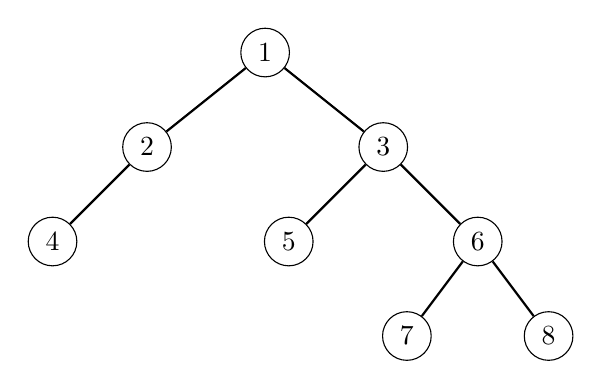
\begin{tikzpicture}[scale=0.6]
\node[draw, circle] (1) at (0,0) {$1$};
\node[draw, circle] (2) at (-2.5,-2) {$2$};
\node[draw, circle] (3) at (2.5,-2) {$3$};
\node[draw, circle] (4) at (-4.5,-4) {$4$};
\node[draw, circle] (5) at (0.5,-4) {$5$};
\node[draw, circle] (6) at (4.5,-4) {$6$};
\node[draw, circle] (7) at (3,-6) {$7$};
\node[draw, circle] (8) at (6,-6) {$8$};
\path[draw,thick,-] (1) -- (2);
\path[draw,thick,-] (1) -- (3);
\path[draw,thick,-] (2) -- (4);
\path[draw,thick,-] (3) -- (5);
\path[draw,thick,-] (3) -- (6);
\path[draw,thick,-] (6) -- (7);
\path[draw,thick,-] (6) -- (8);
\end{tikzpicture}
\caption{Binääripuu, jossa on 8 solmua.}
\label{fig:binpuu}
\end{figure}

Kuvassa \ref{fig:binpuu} on esimerkki binääripuusta, jossa on 8 solmua.
Solmu 1 on puun juuri, ja solmut 4, 5, 7 ja 8 ovat puun lehtiä.
Solmun 3 vasen lapsi on solmu 5, oikea lapsi on solmu 6
ja vanhempi on solmu 1.
Solmun 3 alipuussa ovat solmut 3, 5, 6, 7 ja 8.

Binääripuun juuren \emph{syvyys} on 0 ja jokaisen muun solmun syvyys on yhtä
suurempi kuin sen vanhemman syvyys.
Binääripuun \emph{korkeus} on puolestaan suurin puun solmussa
esiintyvä syvyys.
Esimerkiksi kuvan \ref{fig:binpuu} puun korkeus on 3,
koska solmujen 7 ja 8 syvyys on 3.

\subsection{Binääripuun käsittely}

Voimme toteuttaa binääripuun linkitettynä rakenteena niin,
että jokainen puun solmu on olio, josta on viittaus
solmun vasempaan ja oikeaan lapseen.
Javassa voimme määritellä solmua vastaavan luokan seuraavasti:

\begin{code}
public class Node {
    Node left, right;
    int value;

    public Node(Node left, Node right, int value) {
        this.left = left;
        this.right = right;
        this.value = value;
    }
}
\end{code}

Kentät \texttt{left} ja \texttt{right} osoittavat solmun
vasempaan ja oikeaan lapseen.
Jos lapsi puuttuu, sen tilalla on arvo \texttt{null}.
Kentässä \texttt{value} on puolestaan solmun arvo.
Nyt voimme määritellä kuvan \ref{fig:binpuu} binääripuun näin:

\begin{code}
Node node4 = new Node(null, null, 4);
Node node2 = new Node(node4, null, 2);
Node node7 = new Node(null, null, 7);
Node node8 = new Node(null, null, 8);
Node node6 = new Node(node7, node8, 6);
Node node5 = new Node(null, null, 5);
Node node3 = new Node(node5, node6, 3);
Node node1 = new Node(node2, node3, 1);
\end{code}

Voimme toteuttaa monia binääripuun käsittelyyn liittyviä
operaatioita luontevasti rekursiolla.
Esimerkiksi seuraava metodi laskee, montako solmua
sille annetussa puussa on:

\begin{code}
int laskeSolmut(Node puu) {
    if (puu == null) return 0;
    return 1 + laskeSolmut(puu.left) + laskeSolmut(puu.right);
}
\end{code}

Seuraava metodi puolestaan selvittää, mikä on puun korkeus:

\begin{code}
int korkeus(Node puu) {
    if (puu == null) return -1;
    return 1 + Math.max(korkeus(puu.left), korkeus(puu.right));
}
\end{code}

Huomaa, että jos puu on tyhjä, meidän on kätevää tulkita,
että sen korkeus on $-1$.

\subsection{Läpikäyntijärjestykset}

Voimme käydä läpi binääripuun solmut rekursiivisesti
juuresta alkaen.
Solmujen läpikäyntiin on kolme tavallista järjestystä:

\begin{itemize}
\item \emph{esijärjestys}: käsittelemme ensin solmun, sitten vasemman alipuun
ja lopuksi oikean alipuun
\item \emph{sisäjärjestys}: käsittelemme ensin vasemman alipuun, sitten solmun
ja lopuksi oikean alipuun
\item \emph{jälkijärjestys}: käsittelemme ensin vasemman alipuun,
sitten oikean alipuun ja lopuksi solmun
\end{itemize}

Esimerkiksi kuvan \ref{fig:binpuu} puussa
esijärjestys on $[1,2,4,3,5,6,7,8]$,
sisäjärjes\-tys on $[4,2,1,5,3,7,6,8]$ ja
jälkijärjestys on $[4,2,5,7,8,6,3,1]$.

Seuraava metodi tulostaa binääripuun solmut
sisäjärjestyksessä, kun sille annetaan parametrina
puun juuri.

\begin{code}
void traverse(Node puu) {
    if (puu == null) return;
    traverse(puu.left);
    System.out.println(puu.value);
    traverse(puu.right);
}
\end{code}

\section{Binäärihakupuun toteutus}

Binäärihakupuu on binääripuu, jonka jokainen solmu
on yksi joukon alkioista.
Solmut on järjestetty niin, että jokaisessa solmussa
kaikki arvot vasemmassa alipuussa ovat pienempiä
kuin solmun arvo ja vastaavasti kaikki arvot 
oikeassa alipuussa ovat suurempia.
Tämän ominaisuuden ansiosta voimme löytää helposti
alkion puusta aloittamalla haun puun juuresta.

\begin{figure}
\center
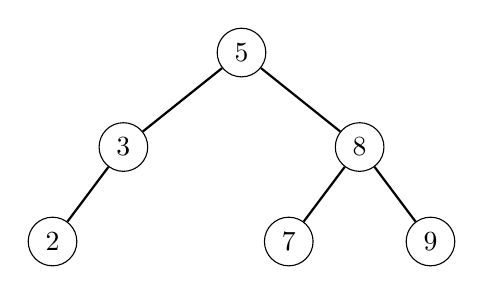
\begin{tikzpicture}[scale=0.6]
\node[draw, circle] (1) at (0,0) {$5$};
\node[draw, circle] (2) at (-2.5,-2) {$3$};
\node[draw, circle] (3) at (2.5,-2) {$8$};
\node[draw, circle] (4) at (-4,-4) {$2$};
\node[draw, circle] (5) at (1,-4) {$7$};
\node[draw, circle] (6) at (4,-4) {$9$};
\path[draw,thick,-] (1) -- (2);
\path[draw,thick,-] (1) -- (3);
\path[draw,thick,-] (2) -- (4);
\path[draw,thick,-] (3) -- (5);
\path[draw,thick,-] (3) -- (6);
\end{tikzpicture}
\caption{Joukkoa $\{2,3,5,7,8,9\}$ vastaava binäärihakupuu.}
\label{fig:bihpuu}
\end{figure}

Kuvassa \ref{fig:bihpuu} on binäärihakupuu,
joka vastaa joukkoa $\{2,3,5,7,8,9\}$.
Tässä tapauksessa puun juuren arvo on 5,
joten vasemmassa alipuussa kaikki arvot
ovat pienempiä kuin 5 ja oikeassa alipuussa
kaikki arvot ovat suurempia kuin 5.
Sama ehto pätee kaikissa muissakin puun solmuissa.

Seuraavaksi käymme läpi, kuinka voimme toteuttaa
haluamamme joukko-operaatiot
binäärihakupuun avulla.
Jokainen operaatio vie aikaa $O(h)$,
missä $h$ on puun korkeus.

\subsection{Joukko-operaatiot}

\subsubsection{Alkion etsiminen}

Kun haluamme löytää puusta solmun $x$, lähdemme liikkeelle
puun juuresta ja kuljemme rekursiivisesti alaspäin puussa.
Kun olemme solmussa, jonka arvo on $a$,
vaihtoehtoja on kolme.
Jos $a=x$, olemme löytäneet halutun solmun,
jos $a<x$, jatkamme hakua solmun oikeaan lapseen,
ja jos $a>x$, jatkamme hakua solmun vasempaan lapseen.
Kuitenkin jos haluttua lasta ei ole, toteamme,
että solmua $x$ ei esiinny puussa.

\begin{figure}
\center
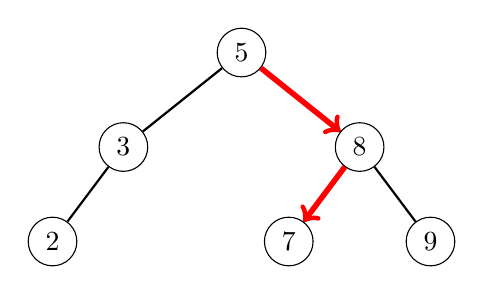
\begin{tikzpicture}[scale=0.6]
\node[draw, circle] (1) at (0,0) {$5$};
\node[draw, circle] (2) at (-2.5,-2) {$3$};
\node[draw, circle] (3) at (2.5,-2) {$8$};
\node[draw, circle] (4) at (-4,-4) {$2$};
\node[draw, circle] (5) at (1,-4) {$7$};
\node[draw, circle] (6) at (4,-4) {$9$};
\path[draw,thick,-] (1) -- (2);
\path[draw,thick,-] (1) -- (3);
\path[draw,thick,-] (2) -- (4);
\path[draw,thick,-] (3) -- (5);
\path[draw,thick,-] (3) -- (6);
\path[draw,thick,red,line width=2pt,->] (1) -- (3);
\path[draw,thick,red,line width=2pt,->] (3) -- (5);
\end{tikzpicture}
\caption{Alkion $7$ etsiminen joukosta $\{2,3,5,7,8,9\}$ juuresta alkaen.}
\label{fig:bihets}
\end{figure}

Kuva \ref{fig:bihets} näyttää, kuinka löydämme alkion 7
joukosta $\{2,3,5,7,8,9\}$.
Juuren arvona on 5, joten alkion täytyy olla juuren
oikeassa alipuussa.
Tämän solmun arvona on 8,
joten nyt taas tiedämme, että alkion täytyy olla
vasemmassa alipuussa, josta se löytyykin.

\subsubsection{Alkion lisääminen}

Kun haluamme lisätä puuhun solmun $x$, kuljemme ensin
puussa aivan kuin etsisimme solmua $x$.
Sitten kun olemme päässeet solmuun,
jolla ei ole lasta, johon meidän tulisi edetä,
lisäämme solmun $x$ tällaiseksi lapseksi.

\begin{figure}
\center
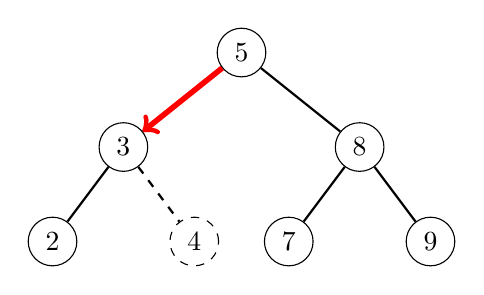
\begin{tikzpicture}[scale=0.6]
\node[draw, circle] (1) at (0,0) {$5$};
\node[draw, circle] (2) at (-2.5,-2) {$3$};
\node[draw, circle] (3) at (2.5,-2) {$8$};
\node[draw, circle] (4) at (-4,-4) {$2$};
\node[draw, circle] (5) at (1,-4) {$7$};
\node[draw, circle] (6) at (4,-4) {$9$};
\node[draw, circle, dashed] (7) at (-1,-4) {$4$};
\path[draw,thick,-] (1) -- (2);
\path[draw,thick,-] (1) -- (3);
\path[draw,thick,-] (2) -- (4);
\path[draw,thick,-] (3) -- (5);
\path[draw,thick,-] (3) -- (6);
\path[draw,thick,dashed,-] (2) -- (7);
\path[draw,thick,red,line width=2pt,->] (1) -- (2);
\end{tikzpicture}
\caption{Alkion 4 lisääminen joukkoon $\{2,3,5,7,8,9\}$.}
\label{fig:bihpu2}
\end{figure}

Kuva \ref{fig:bihpu2} näyttää, kuinka lisäämme alkion 4
joukkoon $\{2,3,5,7,8,9\}$.
Kun haemme puusta solmua 4, päädymme solmuun 3,
jolla ei ole oikeaa lasta.
Niinpä lisäämme solmun 4 solmun 3 oikeaksi lapseksi.

\subsubsection{Alkion poistaminen}

Kun haluamme poistaa puusta solmun $x$, etsimme ensin
solmun $x$ tavalliseen tapaan.
Jos solmulla $x$ ei ole lapsia, poistamme sen vain puusta.
Jos solmulla $x$ on yksi lapsi, korvaamme solmun $x$
sen lapsella.
Jos kuitenkin solmulla $x$ on kaksi lasta,
tilanne on hankalampi.
Tällöin etsimme puusta solmusta $x$ seuraavan
suuremman alkion $y$ (pian kuvattavalla tavalla), vaihdamme keskenään
solmujen $x$ ja $y$ arvot,
ja poistamme sitten solmun $y$.
Solmulla $y$ ei voi olla kahta lasta, joten poistaminen on helppoa.

\begin{figure}
\center
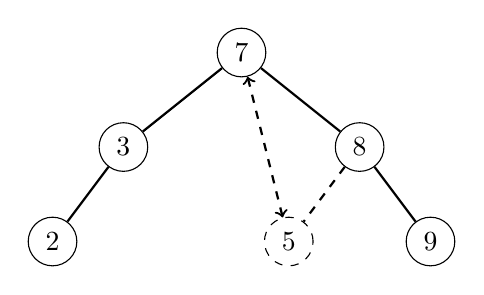
\begin{tikzpicture}[scale=0.6]
\node[draw, circle] (1) at (0,0) {$7$};
\node[draw, circle] (2) at (-2.5,-2) {$3$};
\node[draw, circle] (3) at (2.5,-2) {$8$};
\node[draw, circle] (4) at (-4,-4) {$2$};
\node[draw, circle, dashed] (5) at (1,-4) {$5$};
\node[draw, circle] (6) at (4,-4) {$9$};
\path[draw,thick,-] (1) -- (2);
\path[draw,thick,-] (1) -- (3);
\path[draw,thick,-] (2) -- (4);
\path[draw,thick,-,dashed] (3) -- (5);
\path[draw,thick,-] (3) -- (6);
\path[draw,thick,<->,dashed] (1) -- (5);
\end{tikzpicture}
\caption{Alkion 5 poistaminen joukosta $\{2,3,5,7,8,9\}$.}
\label{fig:bihpu3}
\end{figure}

Kuva \ref{fig:bihpu3} näyttää, kuinka poistamme joukosta $\{2,3,5,7,8,9\}$
alkion 5, joka vastaa binäärihakupuun juurta.
Solmun seuraava suurempi alkio on 7,
joten vaihdamme keskenään arvot 5 ja 7.
Tämän jälkeen meidän on helppoa poistaa solmu puusta.

\subsubsection{Pienin/suurin alkio}

Löydämme puun pienimmän alkion lähtemällä liikkeelle
puun juuresta ja siirtymällä vasempaan lapseen niin
kauan kuin tämä on mahdollista.
Solmu, johon päädymme lopulta, on puun pienin alkio.
Vastaavalla tavalla löydämme suurimman alkion
etenemällä koko ajan oikealle juuresta.

\subsubsection{Seuraava suurempi alkio}

Jos solmulla on oikea lapsi, siirrymme ensin solmusta oikealle
ja sitten vasemmalle niin kauan kuin mahdollista.
Muuten kuljemme solmusta ylöspäin, kunnes saavumme solmuun,
jonka vasen lapsi on edellinen lapsi.
Jos tällaista solmua ei ole, solmulla ei ole seuraavaa
suurempaa alkiota.

\subsubsection{Edellinen pienempi alkio}

Menettelemme käänteisesti edelliseen kohtaan nähden.

\subsection{Operaatioiden tehokkuus}

Binäärihakupuun operaatiot vievät aikaa $O(h)$,
missä $h$ on puun korkeus, joten operaatioiden tehokkuus
riippuu puun korkeudesta.
Niinpä puun tehokkuuteen vaikuttaa, miten olemme
rakentaneet sen.
Esimerkiksi kuvassa \ref{fig:bihkor} on kaksi mahdollista puuta
joukolle $\{1,2,3,4,5\}$.
Vasemman puun korkeus on 3, kun taas oikean puun korkeus on 5.

\begin{figure}
\center
\begin{tikzpicture}[scale=0.6]
\begin{scope}
\node[draw, circle] (1) at (0,0) {$1$};
\node[draw, circle] (2) at (1,-2) {$2$};
\node[draw, circle] (3) at (2,-4) {$3$};
\node[draw, circle] (4) at (3,-6) {$4$};
\node[draw, circle] (5) at (4,-8) {$5$};
\path[draw,thick,-] (1) -- (2);
\path[draw,thick,-] (2) -- (3);
\path[draw,thick,-] (3) -- (4);
\path[draw,thick,-] (4) -- (5);
\end{scope}
\begin{scope}[xshift=-8cm]
\node[draw, circle] (1) at (0,0) {$1$};
\node[draw, circle] (2) at (-2,-2) {$2$};
\node[draw, circle] (3) at (2,-2) {$3$};
\node[draw, circle] (4) at (-4,-4) {$4$};
\node[draw, circle] (5) at (0,-4) {$5$};
\path[draw,thick,-] (1) -- (2);
\path[draw,thick,-] (1) -- (3);
\path[draw,thick,-] (2) -- (4);
\path[draw,thick,-] (2) -- (5);
\end{scope}
\end{tikzpicture}
\caption{Kaksi binäärihakupuuta joukolle $\{1,2,3,4,5\}$.
Vasemman puun korkeus on 3, kun taas oikean puun korkeus on 5.}
\label{fig:bihkor}
\end{figure}


Jotta binäärihakupuu toimii tehokkaasti, haluamme,
että puun korkeus ei kasva liian suureksi.
Tarkemmin ottaen tavoitteemme on, että puun korkeus on
aina vain $O(\log n)$ eli puu on \emph{tasapainoinen}.
Jos onnistumme tässä, kaikki puun operaatiot toimivat
siis tehokkaasti ajassa $O(\log n)$.
Osoittautuu, että saavutamme tavoitteemme
lisäämällä puuhun ehtoja, jotka rajoittavat
sen korkeutta sopivasti.

Binäärihakupuun tasapainottamiseen tunnetaan monia menetelmiä.
Tutustumme seuraavaksi AVL-puuhun, joka on 
varhaisin tunnettu tasapainoinen binäärihakupuu.
AVL-puu on yksinkertaisempi kuin monet myöhemmin
kehitetyt rakenteet, minkä vuoksi se sopii hyvin esittelemään
puiden tasapainotuksen ideoita.
Javan ja muiden ohjelmointikielten standardikirjastoissa
käyte\-tään kuitenkin muita rakenteita, kuten punamustaa puuta.

\section{AVL-puu}

\emph{AVL-puu} on tasapainoinen binäärihakupuu, jonka
korkeus on aina $O(\log n)$, minkä ansiosta puun operaatiot
toimivat tehokkaasti ajassa $O(\log n)$.
AVL-puussa jokaiseen solmuun liittyy \emph{tasapainoehto},
joka takaa, että puu on tasapainoinen.
Kun päivitämme puuta, meidän täytyy pitää huolta siitä,
että tasapainoehto säilyy voimassa kaikissa solmuissa.

\subsection{Tasapainoehto}

AVL-puun tasapainoehto on, että
jokaisessa solmussa vasemman ja oikean lapsen alipuiden korkeusero 
on enintään 1.

Esimerkiksi kuvassa \ref{fig:bihkor} vasen puu on
AVL-puu, kun taas oikea puu ei ole.
Oikea puu ei ole AVL-puu, koska esimerkiksi solmussa 1
vasemman lapsen alipuun korkeus on 0 mutta oikean lapsen
alipuun korkeus on 4.
Korkeuksien erona on siis 4, vaikka ero saisi olla enintään 1.

Kutsumme AVL-puun tasapainoehtoa \emph{AVL-ehdoksi}.
Osoittautuu, että jos binäärihakupuu täyttää AVL-ehdon,
sen korkeus on $O(\log n)$.
Eli jos pystymme toteuttamaan puun operaatiot niin,
että AVL-ehto säilyy, saamme aikaan binäärihakupuun,
jonka operaatiot toimivat ajassa $O(\log n)$.

\begin{figure}
\center
\scriptsize
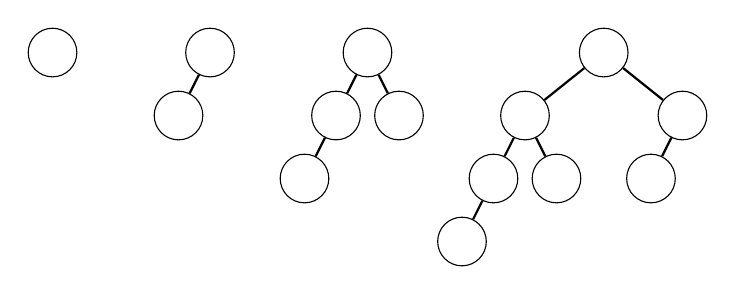
\begin{tikzpicture}[scale=0.4]
\begin{scope}
\node[draw, circle] (2) at (-2.5,-2) {\phantom{$1$}};
\end{scope}
\begin{scope}[xshift=5cm]
\node[draw, circle] (2) at (-2.5,-2) {\phantom{$1$}};
\node[draw, circle] (4) at (-3.5,-4) {\phantom{$1$}};
\path[draw,thick,-] (2) -- (4);
\end{scope}
\begin{scope}[xshift=10cm]
\node[draw, circle] (2) at (-2.5,-2) {\phantom{$1$}};
\node[draw, circle] (4) at (-3.5,-4) {\phantom{$1$}};
\node[draw, circle] (5) at (-1.5,-4) {\phantom{$1$}};
\node[draw, circle] (7) at (-4.5,-6) {\phantom{$1$}};
\path[draw,thick,-] (2) -- (4);
\path[draw,thick,-] (2) -- (5);
\path[draw,thick,-] (4) -- (7);
\end{scope}
\begin{scope}[xshift=15cm,yshift=-2cm]
\node[draw, circle] (1) at (0,0) {\phantom{$1$}};
\node[draw, circle] (2) at (-2.5,-2) {\phantom{$1$}};
\node[draw, circle] (3) at (2.5,-2) {\phantom{$1$}};
\node[draw, circle] (4) at (-3.5,-4) {\phantom{$1$}};
\node[draw, circle] (5) at (-1.5,-4) {\phantom{$1$}};
\node[draw, circle] (6) at (1.5,-4) {\phantom{$1$}};
\node[draw, circle] (7) at (-4.5,-6) {\phantom{$1$}};
\path[draw,thick,-] (1) -- (2);
\path[draw,thick,-] (1) -- (3);
\path[draw,thick,-] (2) -- (4);
\path[draw,thick,-] (2) -- (5);
\path[draw,thick,-] (3) -- (6);
\path[draw,thick,-] (4) -- (7);
\end{scope}
\end{tikzpicture}
\caption{Vähiten solmuja sisältävät AVL-puut korkeuksille 1, 2, 3 ja 4.}
\label{fig:avlkor}
\end{figure}

Miksi sitten AVL-ehto takaa, että binäärihakupuun korkeus
on $O(\log n)$?
Voimme lähestyä asiaa pahimman tapauksen kautta:
kun tiedämme, että AVL-puussa on $n$ solmua,
mikä on sen \emph{suurin mahdollinen} korkeus?
Voimme selvittää tämän tutkimalla käänteisesti,
mikä on \emph{pienin mahdollinen} solmujen määrä
AVL-puussa, jonka korkeus on $h$.

Merkitään $f(h)$:lla korkeutta $h$ olevan AVL-puun
pienintä mahdollista solmujen määrää.
Kuvan \ref{fig:avlkor} mukaisesti funktion ensimmäiset arvot
ovat $f(1)=1$, $f(2)=2$, $f(3)=4$ ja $f(4)=7$.
Yleisemmin
\[f(h)=f(h-1)+f(h-2)+1,\]
koska jos haluamme rakentaa AVL-puun korkeutta $h$,
jossa on mahdollisimman vähän solmuja,
meidän kannattaa laittaa juuren vasempaan
lapseen AVL-puu korkeutta $h-1$ ja oikeaan lapseen
AVL-puu korkeutta $h-2$ niin,
että kummassakin alipuussa on mahdollisimman vähän solmuja.

Kun $h \ge 3 $, funktiolle pätee
\[f(h) \ge 2 f(h-2),\]
eli funktion arvo ainakin kaksinkertaistuu kahden askeleen välein.
Voimme esittää tämän alarajan muodossa
\[f(h) \ge 2^{h/2},\]
joka taas tarkoittaa samaa kuin
\[ h \le 2 \log_2 f(h).\]

Tarkastellaan sitten puuta, jossa on $n$ solmua.
Puun korkeudelle $h$ täytyy päteä $f(h) \le n$,
koska korkeutta $h$ olevassa puussa on vähintään $f(h)$ solmua.
Niinpä saamme alarajan
\[h \le 2 \log_2 n,\]
mikä tarkoittaa samaa kuin $h = O(\log n)$.

\subsection{Kiertojen toteutus}

TODO

\section{Javan rakenteet}

Javassa on binäärihakupuuhun pohjautuvat rakenteet
\texttt{TreeSet} ja \texttt{TreeMap},
jotka muistuttavat rakenteita \texttt{HashSet} ja \texttt{HashMap}.
Erona on kuitenkin, että pystymme etsimään
alkioita niiden järjestyksen perusteella.

\subsection{\texttt{TreeSet}-rakenne}

Seuraava koodi luo \texttt{TreeSet}-rakenteen,
joka pitää yllä lukujen joukkoa.
Koodi lisää joukkoon alkioita ja tulostaa sitten sen sisällön.

\begin{code}
TreeSet<Integer> joukko = new TreeSet<>();
joukko.add(4);
joukko.add(1);
joukko.add(8);
joukko.add(7);
System.out.println(joukko); // [1, 4, 7, 8]
\end{code}

Koska joukko on järjestyksessä, pystymme etsimään tehokkaasti
pienim\-män ja suurimman alkion metodeilla \texttt{first} ja \texttt{last}:

\begin{code}
System.out.println(joukko.first()); // 1
System.out.println(joukko.last()); // 8
\end{code}

Pystymme myös etsimään seuraavan tiettyä alkiota
suuremman tai pienemmän alkion metodeilla \texttt{higher} ja \texttt{lower}:

\begin{code}
System.out.println(joukko.higher(5)); // 7
System.out.println(joukko.lower(5)); // 4
\end{code}

Kaikki nämä operaatiot toimivat ajassa $O(\log n)$.

\subsection{\texttt{TreeMap}-rakenne}

Seuraava koodi luo sanakirjan \texttt{TreeMap}-rakenteen avulla:

\begin{code}
TreeMap<String,String> sanakirja = new TreeMap<>();
sanakirja.put("apina","monkey");
sanakirja.put("banaani","banana");
sanakirja.put("cembalo","harpsichord");
\end{code}

Tässä tapauksessa rakenteen avaimet on järjestetty,
joten pystymme etsimään tietoa avainten perusteella.
Esimerkiksi voimme selvittää, mikä on aakkosjärjestyksessä
ensimmäinen ja viimeinen sanakirjassa oleva sana:

\begin{code}
System.out.println(sanakirja.firstKey()); // apina
System.out.println(sanakirja.lastKey()); // cembalo
\end{code}

Samoin voimme selvittää lähinnä tiettyä avainta olevat avaimet:

\begin{code}
System.out.println(sanakirja.higherKey("bonus")); // cembalo
System.out.println(sanakirja.lowerKey("bonus")); // banaani
\end{code}

\subsection{Omat luokat}

TODO

\section{Tehokkuusvertailu}

Monissa ongelmissa meillä on kaksi mahdollista lähestymistapaa:
voimme käyttää joukkorakenteita tai taulukoita ja järjestämistä.
Vaikka molemmat tavat johtavat tehokkaaseen ratkaisuun,
vakiokertoimissa voi olla merkittäviä eroja, jotka vaikuttavat
käytännön tehokkuuteen.

Keskitymme seuraavaksi ongelmaan, jossa meille on annettu
$n$ lukua sisältävä taulukko, ja haluamme selvittää,
montko eri lukua taulukossa on.
Ratkaisemme ongelman kolmella eri tavalla ja tutkimme sitten
ratkaisujen tehokkuutta.

\subsubsection{Ratkaisu 1: \texttt{TreeSet}}

Ensimmäinen tapa ratkaista tehtävä on luoda \texttt{TreeSet},
johon lisäämme kaikki taulukon luvut.
Koska jokainen luku voi esiintyä joukossa enintään kerran,
joukon koko ilmaisee meille, montako eri lukua taulukossa on.

\begin{code}
int eriLuvut(int[] taulu) {
    TreeSet<Integer> joukko = new TreeSet<>();
    for (int i = 0; i < taulu.length; i++) {
        joukko.add(taulu[i]);
    }
    return joukko.size();
}
\end{code}

\subsubsection{Ratkaisu 2: \texttt{HashSet}}

Emme tarvitse ratkaisussa \texttt{TreeSet}-rakenteen
tarjoamaa alkioiden järjestystä, joten voimme käyttää
yhtä hyvin \texttt{HashSet}-rakennetta.
Koodi säilyy muuten täysin samanlaisena.

\begin{code}
int eriLuvut(int[] taulu) {
    HashSet<Integer> joukko = new HashSet<>();
    for (int i = 0; i < taulu.length; i++) {
        joukko.add(taulu[i]);
    }
    return joukko.size();
}
\end{code}

\subsubsection{Ratkaisu 3: järjestäminen}

Kolmas tapa ratkaista tehtävä on käyttää järjestämistä:
laitamme luvut listaan, järjestämme listaan ja
tutkimme, monessako kohdassa järjestetyllä listalla
luku vaihtuu.

\begin{code}
int eriLuvut(int[] taulu) {
    int[] lista = taulu.clone();
    Arrays.sort(lista);
    int tulos = 1;
    for (int i = 1; i < lista.length; i++) {
        if (lista[i-1] != lista[i]) tulos++;
    }
    return tulos;
}
\end{code}

\subsubsection{Vertailun tulokset}

Taulukko \ref{tab:eriver} esittää tehokkuusvertailun tulokset,
kun taulukon koko $n$ vaihtelee.
Jokaisessa testissä taulukko muodostettiin satunnaisesti niin,
että sen luvut ovat välillä $1 \dots 10^9$.

Osoittautuu, että ratkaisujen välillä on merkittäviä tehokkuuseroja.
Ensinnäkin \texttt{HashSet}-ratkaisu on noin kolme kertaa
nopeampi kuin \texttt{TreeSet}-ratkaisu.
Tämä on siinä mielessä odotettavaa, että hajautustaulun
operaatiot vievät aikaa $O(1)$, kun taas binäärihakupuun
operaatiot vievät aikaa $O(\log n)$.
Selvästi nopein ratkaisu on kuitenkin kolmas järjestämistä
käyttävä ratkaisu, joka on noin kymmenen kertaa
\texttt{TreeSet}-ratkaisua nopeampi.

Kiinnostava seikka on, että sekä \texttt{TreeSet}-ratkaisu että
järjestämisratkaisu vievät aikaa $O(n \log n)$, mutta
jälkimmäinen ratkaisu on kymmenen kertaa nopeampi.
Tämä johtuu siitä, että taulukon järjestäminen on hyvin kevyt
operaatio, ja se tehdään vain kerran.
Binäärihakupuussa jokaisen lisäyksen jälkeen täytyy muuttaa
puun rakennetta, mikä on hidasta ja aiheuttaa suuret vakiokertoimet.

Vaikka joukkorakenteet ovat käteviä, niitä ei siis kannata
käyttää turhaan.
Joukkorakenteiden etuna on, että alkioiden lisääminen ja poistaminen
toimivat tehokkaasti.
Jos tällaiselle ei ole tarvetta, järjestämiseen perustuva ratkaisu
saattaa olla parempi valinta.

\begin{table}
\center
\begin{tabular}{rrrr}
taulukon koko $n$ & \texttt{TreeSet} & \texttt{HashSet} & järjestäminen \\
\hline
$10^6$ & 0.74 s & 0.25 s & 0.09 s \\
$2 \cdot 10^6$ & 1.60 s & 0.45 s & 0.19 s \\
$4 \cdot 10^6$ & 5.60 s & 1.56 s & 0.52 s \\
$8 \cdot 10^6$ & 12.19 s & 4.50 s & 0.97 s \\
\end{tabular}
\caption{Algoritmien suoritusaikojen vertailu.}
\label{tab:eriver}
\end{table}

\chapter{Algoritmien suunnittelu}

Kuinka voi suunnitella hyvän algoritmin?
On selvää, ettei tähän kysymykseen ole yhtä helppoa vastausta.
Yhtä hyvin voisi kysyä, kuinka voi kirjoittaa hyvän kirjan
tai säveltää hyvää musiikkia.
Algoritmien suunnittelu on taito, jonka oppiminen vie aikaa.

Algoritmisen ongelman ratkaisemisessa on usein kaksi vaihetta.
Ensim\-mäinen vaihe on keksiä algoritmin yleisidea,
mikä vaatii havaintoja ja oivalluksia ongelmasta.
Tämän jälkeen toinen vaihe on löytää hyvä ja tehokas tapa
toteuttaa algoritmi.
Tässä voimme käyttää apuna järjestämistä, tietorakenteita
ja muita tekniikoita.

Kuten aiemminkin, haluamme saada aikaan tehokkaita algoritmeja,
jotka vievät aikaa $O(n)$ tai $O(n \log n)$.
Tämä tarkoittaa käytännössä sitä, että voimme käydä läpi ja
järjestää syötettä sekä käyttää tietorakenteita,
joissa on tehokkaita operaatioita.
Tämä rajaa sitä, mitä voimme tehdä algoritmissa, ja ohjaa
algoritmin suunnittelua.

\section{Ratkaisun vaiheet}

Tarkastellaan esimerkkinä tehtävää,
jossa $n$ lasta haluaa mennä maailmanpyörään.
Jokaisessa korissa voi istua yksi tai kaksi lasta.
Tiedämme jokaisen lapsen painon,
ja jokaisessa korissa suurin istujien
yhteispaino saa olla $x$.
Mikä on pienin mahdollinen määrä koreja,
joka riittää lapsille?
Oletamme, ettei yhdenkään lapsen paino ylitä
korin maksimipainoa.

Esimerkiksi jos lasten määrä on $n=5$,
lasten painot ovat $[2,2,4,5,8]$ ja korin painoraja on $x=8$,
pienin mahdollinen korien määrä on kolme.
Tässä tapauksessa voimme muodostaa korit
$[2,4]$, $[2,5]$ ja $[8]$.
Tämä on optimaalinen ratkaisu, koska selvästikään
ei riitä, että koreja olisi vain kaksi.

\subsubsection{Vaihe 1: Yleisidean keksiminen}

On valtava määrä mahdollisia tapoja,
miten voimme sijoittaa lapsia koreihin,
minkä vuoksi olisi liian hidasta käydä läpi
kaikkia vaihtoehtoja.
Jotta saamme aikaan tehokkaan algoritmin,
meidän tulee keksiä jokin periaate,
jonka avulla voimme päättää nopeasti,
ketkä lapset ovat yhdessä koreissa.

Itse asiassa meidän riittää keskittyä ongelmaan,
jossa haluamme löytää \emph{seuraavaan} koriin
tulevat lapset.
Jos onnistumme tässä, voimme vain toistaa samaa,
kunnes kaikki lapset ovat koreissa.
Vaikeutena on kuitenkin, kuinka saamme tehtyä valinnan niin,
että tuloksena on varmasti optimaalinen ratkaisu.
Jos valitsemme väärällä tavalla koriin tulevat lapset,
saatamme vahingossa käyttää liikaa koreja.

Osoittautuu, että tässä tehtävässä toimiva algoritmi
on valita aina seuraavaan koriin \emph{painavin} lapsi sekä sen pariksi
jokin toinen lapsi niin, että painojen summa ei ylitä
korin maksimipainoa.
Jos ei ole mitään tapaa valita toista lasta,
laitamme painavimman lapsen koriin yksin.
Tällainen algoritmi on \emph{ahne}, eli se tekee aina jonkin
hyvältä tuntuvan valinnan, joka vie ratkaisua eteenpäin,
eikä peruuta koskaan tehtyjä valintoja.

Tarkastellaan taas esimerkkiä,
jossa lasten painot ovat $[2,2,4,5,8]$
ja korin maksimipaino on 8.
Kun käytämme yllä kuvattua algoritmia,
aloitamme lapsesta, jonka paino on 8.
Tämä lapsi saa oman korin, koska emme voi laittaa
samaan koriin ketään toista lasta.
Tämän jälkeen vuoroon tulee lapsi, jonka paino on 5,
ja se saa pariksi lapsen, jonka paino on 2.
Lopuksi käsittelemme lapsen, jonka paino on 4,
ja sen pariksi tulee lapsi, jonka paino on 2.
Tuloksena on ratkaisu, jossa on korit $[8]$, $[2,5]$ ja $[2,4]$.

Mutta miksi tämä ahne algoritmi toimii?
Tässä auttaa tarkastella, mitä tapahtuu,
kun algoritmi tekee ensimmäisen valintansa.
Painavin lapsi täytyy sijoittaa johonkin koriin,
ja meidän kannattaa tietenkin laittaa samaan koriin toinenkin lapsi,
jos tämä on mahdollista.
Tässä ei ole väliä, minkä toisen lapsen valitsemme,
koska jos jokin lapsi on riittävän kevyt toimiakseen
parina painavimman lapsen kanssa, niin se voi toimia parina
myös minkä tahansa muun lapsen kanssa.
Niinpä algoritmin ensimmäinen askel on optimaalinen.
Tämän jälkeen voimme toistaa vastaavan päättelyn
algoritmin seuraavissa askelissa, mikä tarkoittaa,
että koko algoritmi toimii oikein.

\subsubsection{Vaihe 2: Tehokas toteutus}

Meillä on nyt toimiva algoritmi,
mutta meidän täytyy vielä keksiä hyvä tapa toteuttaa se.
Jotta algoritmista tulee tehokas,
meidän tulee joka askeleella löytää nopeasti seuraavaan
koriin tuleva painavin lapsi sekä mahdollinen sen pariksi tuleva lapsi.
Ehkä helpoin tapa saavuttaa tämä tavoite on käyttää apuna järjestämistä.

Seuraava algoritmi järjestää ensin lasten painot ja alkaa sitten
jakaa lapsi koreihin.
Muuttuja $a$ lähtee liikkeelle taulukon alusta ja
osoittaa aina kevyimmän lapsen painoon.
Muuttuja $b$ puolestaan lähtee liikkeelle taulukon lopusta ja
osoittaa aina painavimman lapsen painoon.
Algoritmi laskee muuttujaan $k$, montako koria tarvitaan yhteensä.
Jos kevyimmän ja painavimman lapsen
painojen summa on enintään $x$, lapset sijoitetaan samaan koriin,
$a$ liikkuu oikealle ja $b$ liikkuu vasemmalle.
Jos taas painojen summa on suurempi kuin $x$,
painavin lapsi saa oman korin ja vain $b$ liikkuu vasemmalle.

\begin{code}
sort(painot)
a = 0, b = n-1
k = 0
while a <= b
    if painot[a]+painot[b] <= x
        a++, b--
    else
        b--
    k++
print(k)
\end{code}

Algoritmi järjestää ensin taulukon, missä menee aikaa $O(n \log n)$.
Tämän jälkeen \texttt{while}-silmukka vie aikaa $O(n)$,
koska joka kierroksella muuttujat $a$ ja $b$ siirtyvät
ainakin askeleen lähemmäs toisiaan.
Niinpä algoritmin kokonais\-aikavaativuus on $O(n \log n)$.

\section{Algoritmien aineksia}

Seuraavaksi käymme läpi \emph{aineksia},
joita esiintyy usein tehokkaissa algoritmeissa.
Nämä ainekset muodostavat hyvän perustan algoritmien
suunnittelemiseen: kun saamme vastaamme uuden ongelman,
voimme miettiä, voisimmeko hyödyntää aineksia jotenkin
ongelman ratkaisemisessa.

\subsection{Järjestäminen}

Tehokas algoritmi perustuu usein tavalla tai
toisella järjestämiseen, joka voi näyttäytyä
monella tavalla algoritmissa.

Tarkastellaan esimerkkinä tehtävää, jossa annettuna on
$n$ kolikkoa ja haluamme löytää pienimmän rahamäärän,
jota \emph{emme} voi muodostaa summana kolikoista.
Jokaisella kolikolla on tietty kokonaislukuarvo, ja
muodostettava rahamäärä on myös kokonaisluku.
Esimerkiksi jos kolikot ovat $[1,2,2,7]$,
voimme muodostaa rahamäärät 1, 2, 3, 4 ja 5,
mutta emme voi muodostaa rahamäärää 6,
joten oikea vastaus on 6.

Algoritmien suunnittelussa auttaa usein
lähteä liikkeelle helpoista tapauksista.
Kun meillä on käytössämme tietyt kolikot,
hyvä ensimmäinen tavoite on koettaa muodostaa rahamäärä $1$.
Jotta onnistumme tässä, meillä on pakko olla kolikko,
jonka arvo on $1$.
Entä milloin voimme muodostaa rahamäärän $2$,
jos tiedämme, että voimme muodostaa rahamäärän $1$?
Tässä on kaksi vaihtoehtoa: meillä täytyy olla
toinen kolikko, jonka arvo on $1$, jolloin saamme
summan $1+1=2$, tai sitten kolikko, jonka arvo on $2$.

Tämä on hyvää päättelyä, mutta jotta saamme aikaan algoritmin,
meidän täytyy pystyä yleistämään se kaikkiin tapauksiin.
Voimme ajatella asiaa hieman toisesta näkökulmasta:
Meillä on joukko kolikoita, joiden avulla voimme muodostaa
rahamäärät $1,2,\dots,k$.
Miten voisimme muodostaa myös rahamäärän $k+1$?
Ratkaisu on, että tarvitsemme uuden kolikon,
jonka arvo on \emph{enintään} $k+1$.
Kun uuden kolikon arvo on $u \le k+1$,
voimme tämän jälkeen muodostaa rahamäärät $1,2,\dots,k+u$.
Tämän havainnon ansiosta voimme alkaa muodostaa ratkaisua
kolikko kerrallaan.
Lisäksi jos mahdollisia uusia kolikoita on useita,
voimme aina valita ahneesti \emph{pienimmän} kolikon,
koska pystymme valitsemaan suuremmat kolikot myöhemminkin.

Nyt meillä on kaikki ainekset tehokasta algoritmia varten.
Järjes\-tämme ensin kolikot ja muodostamme sitten ratkaisun
käymällä kolikot läpi pienimmästä suurimpaan.
Aloitamme tyhjästä ratkaisusta, jossa $k=0$.
Jokaisen kolikon kohdalla tiedämme,
että voimme muodostaa tällä hetkellä rahamäärät $1,2,\dots,k$,
joten voimme parantaa ratkaisua kolikon avulla,
jos sen arvo on enintään $k+1$.
Muuten lopetamme ratkaisun muodostamisen,
koska kaikki tulevat kolikot ovat vielä suurempia.
Lopuksi toteamme, että $k+1$ on pienin rahamäärä,
jota emme voi muodostaa.

\begin{code}
sort(kolikot)
k = 0
for i = 0 to n-1
    u = kolikot[i]
    if u <= k+1
        k += u
    else
        break
print(k+1)
\end{code}

Algoritmi järjestää ensin kolikot ajassa $O(n \log n)$
ja tämän jälkeen käy ne läpi ajassa $O(n)$,
joten algoritmin aikavaativuus on $O(n \log n)$.

\subsection{Tietorakenteet}

Olemme tutustuneet kirjassa jo moniin tietorakenteisiin:
listaan, hajautustauluun, binäärihakupuuhun ja kekoon.
Näissä tietorakenteissa kannattaa kiinnittää erityisesti huomiota siihen,
mitkä operaatiot toimivat tehokkaasti $O(1)$- tai $O(\log n)$-ajassa.
Nämä ovat operaatioita, joita voimme käyttää tehokkaissa algoritmeissa.

Tarkastellaan esimerkkinä tehtävää, jossa haluamme laskea,
montako tapaa on valita taulukosta yhtenäinen osataulukko,
jossa lukujen summa on $x$.
Esimerkiksi jos taulukko on $[3,1,3,4,5]$ ja $x=4$,
niin tapoja on kolme: $[3,1]$, $[1,3]$ ja $[4]$.
On helppoa ratkaista tehtävä kahdella silmukalla ajassa $O(n^2)$,
mutta miten saisimme aikaan tehokkaan algoritmin?

Tässä auttaa muotoilla hieman toisin, mitä tarkoittaa,
että osataulukolla on tietty summa.
Merkitään $s(i)$:llä osataulukon summaa taulukon alusta
kohtaan $i$ asti, ja oletetaan lisäksi, että $s(-1)=0$.
Tätä merkintää käyttäen osataulukon summa
kohdasta $a$ kohtaan $b$ on
\[s(b)-s(a-1),\]
eli meidän riittää itse asiassa keskittyä vain taulukon alusta
alkavien osataulukoiden summiin.

Koska haluamme saada tehokkaan algoritmin,
hyvä tavoite olisi käydä taulukko läpi vain kerran.
Kun olemme taulukon kohdassa $i$,
monessako tähän kohtaan päättyvässä osataulukossa
lukujen summa on $x$?
Tämä tarkoittaa, että haluamme etsiä kohdat $j \le i$,
joille pätee
\[s(i)-s(j-1)=x\]
eli
\[s(j-1)=s(i)-x.\]
Saamme laskettua tällaisten kohtien määrän tehokkaasti,
kun pidämme taulukon läpikäynnissä kirjaa,
montako kertaa mikäkin summa on esiintynyt taulukon alkuosassa.
Voimme toteuttaa algoritmin seuraavasti:

\begin{code}
summat[0] = 1
laskuri = 0
summa = 0
for i = 0 to n-1
    summa += taulu[i]
    laskuri += summat[summa-x]
    summat[summa]++
print(laskuri)
\end{code}

Joka askeleella muuttuja \texttt{summa} sisältää
summan $s(i)$.
Rakenne \texttt{summat} pitää kirjaa,
montako kertaa mikäkin alkuosan summa on esiintynyt tähän mennessä.
Koska summat voivat olla suuria, tavallinen taulukko ei kelpaa,
mutta voimme käyttää hajautustauluun tai binäärihakupuuhun
perustuvaa hakemistoa.
Näin saamme aikaan ratkaisun, joka vie aikaa $O(n)$ tai $O(n \log n)$
riippuen valitusta tietorakenteesta.

\subsection{Binäärihaku}

Binäärihaun tunnetuin käyttötarkoitus on alkion etsiminen
järjestetystä taulukosta ajassa $O(\log n)$.
Tämä on kuitenkin vain alkusoittoa sille,
mitä binää\-rihaulla pystyy tekemään ja mikä on sen
merkitys algoritmien suunnittelussa.
Binääri\-haun todellinen hyöty piilee siinä,
että pystymme etsimään sen avulla tehokkaasti funktion \emph{muutoskohdan}.

Oletetaan, että meillä on funktio $\texttt{ok}(x)$,
joka kertoo, onko $x$ kelvollinen ratkaisu tehtävään.
Lisäksi pätee $\texttt{ok}(x)=\texttt{false}$, kun $x<k$,
ja $\texttt{ok}(x)=\texttt{true}$, kun $x \ge k$.
Binäärihaun avulla voimme etsiä tehokkaasti,
mikä on funktion muutoskohta $k$
eli ensimmäinen kohta, jossa funktio saa arvon \texttt{true}.
Seuraava koodi toteuttaa haun, kun oletamme, että $k$ on välillä $1 \dots N$:

\begin{code}
a = 1, b = N
while a < b
    u = (a+b)/2
    if ok(u)
        b = u
    else
        a = u+1
k = a
\end{code}

Haun joka vaiheessa tiedämme, että muutoskohta on välillä $[a,b]$.
Laskemme keskikohdan $u=\lfloor (a+b)/2 \rfloor$ ja tutkimme funktion arvoa kohdassa $u$.
Jos pätee $\texttt{ok}(u)$, niin muutoskohdan on oltava välillä $[a,u]$,
ja muuten sen täytyy olla välillä $[u+1,b]$.
Lopulta välillä on vain yksi alkio, jolloin olemme löytäneet muutoskohdan.
Koska välin koko puolittuu joka askeleella,
kutsumme funktiota \texttt{ok} yhteensä $O(\log N)$ kertaa.

\begin{figure}
\center
\begin{tikzpicture}[scale=0.6]
\draw[->] (-1,1.5) -- (10,1.5);
\foreach \x in {0,...,8} \draw (\x,1.40) -- (\x,1.60);
\foreach \x in {0,...,8} \node at (\x,2) {\scriptsize $\x$};
\node at (-2,0) {kone $1$};
\draw[|-|] (0.05,0) -- (1.95,0);
\draw[|-|] (2.05,0) -- (3.95,0);
\draw[|-|] (4.05,0) -- (5.95,0);
\draw[|-|] (6.05,0) -- (7.95,0);
\node at (-2,-1.5) {kone $2$};
\draw[|-|] (0.05,-1.5) -- (2.95,-1.5);
\draw[|-|] (3.05,-1.5) -- (5.95,-1.5);
\node at (-2,-3) {kone $3$};
\draw[|-|] (0.05,-3) -- (6.95,-3);
\end{tikzpicture}
\caption{Optimaalinen tapa valmistaa 7 tavaraa vie 8 minuuttia,
kun koneiden nopeudet ovat $[2,3,7]$.}
\label{fig:optkon}
\end{figure}

Mutta mitä hyötyä on siitä, että löydämme tehokkaasti funktion muutoskohdan?
Tämä selviää seuraavassa tehtävässä:
Käytössämme on $n$ konetta
ja haluamme valmistaa niiden avulla $m$ tavaraa.
Tiedämme jokaisesta koneesta,
montako minuuttia kestää valmistaa yksi tavara konetta käyttäen,
ja haluamme löytää aikataulun, jota seuraamalla pystymme valmistamaan
$m$ tavaraa mahdollisimman nopeasti.

Kuva \ref{fig:optkon} näyttää parhaan aikataulun esimerkkitilanteessa,
jossa koneiden nopeudet ovat $[2,3,7]$ ja haluamme
valmistaa seitsemän tavaraa (eli $m=7$).
Käynnistämme koneen 1 neljästi kahden minuutin välein,
koneen 2 kahdesti kolmen minuutin välein ja koneen 3 kerran.
Viimeisenä pysähtyy kone 1, kun aloittamisesta
on kulunut kahdeksan minuuttia.

Voimme pukea tehtävän binäärihaulle sopivaan muotoon määrittämällä,
että $\texttt{ok}(x)=\texttt{true}$ tarkalleen silloin, kun voimme valmistaa
\emph{ainakin} $m$ tavaraa ajassa $x$.
Tällöin funktion muutoskohta $k$ vastaa tehtävän ratkaisua.
Entä miten voimme laskea funktion \texttt{ok} arvon?
Jos meillä on $u$ minuuttia aikaa ja koneella $i$ kestää $x_i$
minuuttia valmistaa yksi tavara, pystymme valmistamaan
$\lfloor u/x_i \rfloor$ tavaraa kyseistä konetta käyttäen.
Kun sitten käytössämme on kaikki koneet,
pystymme valmistamaan yhteensä
\[ s = \sum_{i=1}^n \lfloor u/x_i \rfloor \]
tavaraa. Niinpä $\texttt{ok}(u)=\texttt{false}$, jos $s<m$,
ja $\texttt{ok}(u)=\texttt{true}$, jos $s \ge m$.
Voimme toteuttaa tämän käytännössä seuraavasti:

\begin{code}
function ok(u)
    s = 0
    for i = 1 to n
        s += u/x[i]
    return s >= m
\end{code}

Voimme kytkeä tämän funktion suoraan binäärihakuun,
jolloin tuloksena on tehokas algoritmi tehtävän ratkaisemiseen.
Meidän täytyy kuitenkin vielä valita arvo $N$,
joka on jokin yläraja kohdalle $k$.
Tässä tehtävässä helppo valinta on
\[N = x_1 \cdot m,\]
mikä vastaa ratkaisua, jossa käytämme vain ensimmäistä konetta.
On varmaa, että oikea $k$:n arvo on korkeintaan $N$,
joten binäärihaku kutsuu $O(\log N)$ kertaa funktiota $\texttt{ok}$.
Koska jokainen funktion kutsu vie aikaa $O(n)$,
tuloksena on algoritmi, jonka aikavaativuus on $O(n \log N)$.

Huomaa, että $\log N$ on käytännössä pieni luku riippumatta
siitä, kuinka suuri luku $N$ on.
Niinpä meidän ei tarvitse murehtia siitä,
kuinka suuria $x_1$ ja $m$ ovat,
vaan voimme luottaa siihen, että algoritmi on tehokas.

\subsection{Tasoitettu analyysi}

Voimme yleensä määrittää algoritmin aikavaativuuden
helposti katsomalla jokaisesta silmukasta,
montako kertaa siinä olevaa koodia suoritetaan.
Joskus näin suoraviivainen analyysi ei anna kuitenkaan
oikeaa kuvaa algoritmin tehokkuudesta,
koska silmukan suorituskertojen määrä saattaa vaihdella
algoritmin eri vaiheissa.
Tutustumme seuraavaksi tekniikkaan nimeltä
\emph{tasoitettu analyysi}, jossa koetamme arvioida tarkemmin,
montako kertaa silmukassa olevaa koodia suoritetaan
\emph{yhteensä} algoritmin aikana.

Tasoitettuun analyysiin liittyy yleensä jokin tietorakenne,
jonka operaatioiden määrää haluamme arvioida.
Tarkastellaan esimerkkinä tehtävää,
jossa meillä on $n$ lukua sisältävä taulukko
ja haluamme muodostaa toisen taulukon,
jossa on jokaisen luvun \emph{lähin pienempi edeltäjä}.
Tämä tarkoittaa, että haluamme löytää jokaiselle luvulle
pienemmän luvun, joka on mahdollisimman lähellä aiemmin taulukossa.
Esimerkiksi taulukon $[1,4,5,2,3,2]$
lähimmät pienemmät edeltäjät ovat $[-,1,4,1,2,1]$.
Koska luvulla $1$ ei ole pienempää edeltäjää,
sen kohdalla on merkki $-$.

\begin{figure}
\center
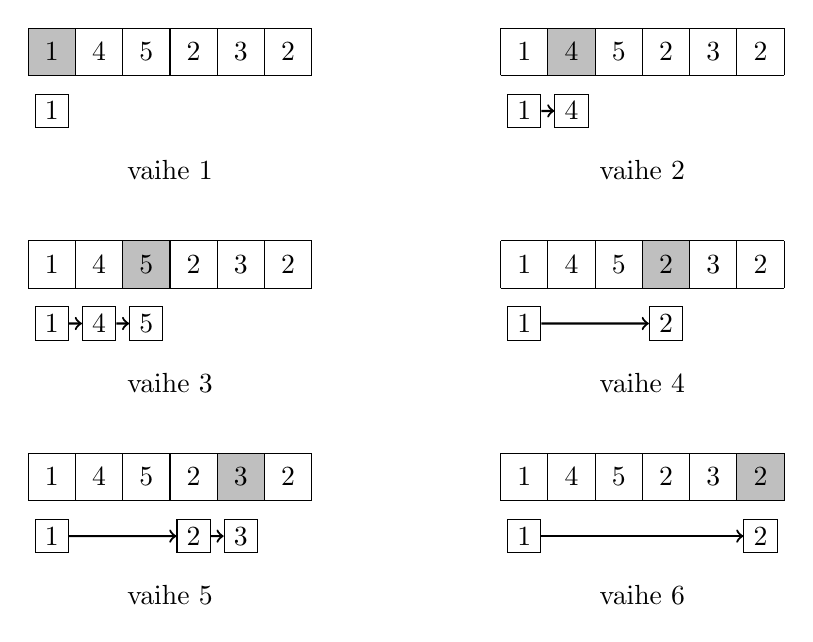
\begin{tikzpicture}[scale=0.6]
\newcommand\pino[3]{
\node[draw,rectangle,minimum size=12pt] (#1) at (#2+0.5,-0.75) {};
\node at (#2+0.5,-0.75) {#3};
}
\begin{scope}
\fill[color=lightgray] (0,0) rectangle (1,1);
\draw (0,0) grid (6,1);
\foreach \i/\x in {0/1,1/4,2/5,3/2,4/3,5/2} \node at (\i+0.5,0.5) {\x};
\pino{1}{0}{1}
\node at (3,-2) {vaihe $1$};
\end{scope}
\begin{scope}[xshift=10cm]
\fill[color=lightgray] (1,0) rectangle (2,1);
\draw (0,0) grid (6,1);
\foreach \i/\x in {0/1,1/4,2/5,3/2,4/3,5/2} \node at (\i+0.5,0.5) {\x};
\pino{1}{0}{1}
\pino{2}{1}{4}
\draw[thick,->] (1) -- (2);
\node at (3,-2) {vaihe $2$};
\end{scope}
\begin{scope}[yshift=-4.5cm]
\fill[color=lightgray] (2,0) rectangle (3,1);
\draw (0,0) grid (6,1);
\foreach \i/\x in {0/1,1/4,2/5,3/2,4/3,5/2} \node at (\i+0.5,0.5) {\x};
\pino{1}{0}{1}
\pino{2}{1}{4}
\pino{3}{2}{5}
\draw[thick,->] (1) -- (2);
\draw[thick,->] (2) -- (3);
\node at (3,-2) {vaihe $3$};
\end{scope}
\begin{scope}[yshift=-4.5cm,xshift=10cm]
\fill[color=lightgray] (3,0) rectangle (4,1);
\draw (0,0) grid (6,1);
\foreach \i/\x in {0/1,1/4,2/5,3/2,4/3,5/2} \node at (\i+0.5,0.5) {\x};
\pino{1}{0}{1}
\pino{2}{3}{2}
\draw[thick,->] (1) -- (2);
\node at (3,-2) {vaihe $4$};
\end{scope}
\begin{scope}[yshift=-9cm]
\fill[color=lightgray] (4,0) rectangle (5,1);
\draw (0,0) grid (6,1);
\foreach \i/\x in {0/1,1/4,2/5,3/2,4/3,5/2} \node at (\i+0.5,0.5) {\x};
\pino{1}{0}{1}
\pino{2}{3}{2}
\pino{3}{4}{3}
\draw[thick,->] (1) -- (2);
\draw[thick,->] (2) -- (3);
\node at (3,-2) {vaihe $5$};
\end{scope}
\begin{scope}[yshift=-9cm,xshift=10cm]
\fill[color=lightgray] (5,0) rectangle (6,1);
\draw (0,0) grid (6,1);
\foreach \i/\x in {0/1,1/4,2/5,3/2,4/3,5/2} \node at (\i+0.5,0.5) {\x};
\pino{1}{0}{1}
\pino{2}{5}{2}
\draw[thick,->] (1) -- (2);
\node at (3,-2) {vaihe $6$};
\end{scope}
\end{tikzpicture}
\caption{Etsimme lähimmät pienemmät edeltäjät pinon avulla.}
\label{fig:pielah}
\end{figure}

Saamme ratkaistua tehtävän tehokkaasti algoritmilla,
joka käy läpi taulukkoa vasemmalta oikealle ja pitää yllä \emph{pinoa},
jossa on lista taulukon lukuja.
Pino on muodostettu niin, että jokainen alkio on edellistä suurempi.
Jokaisessa kohdassa $i$ poistamme ensin pinon lopusta lukuja
niin kauan kuin pinon viimeinen luku on suurempi tai yhtä
suuri kuin kohdan $i$ luku.
Tämän jälkeen kirjaamme muistiin, että kohdan $i$ luvun
lähin pienempi edeltäjä on pinon viimeinen luku (jos pino ei ole tyhjä) ja
lisäämme kohdan $i$ luvun pinon loppuun.
Tuloksena on seuraava algoritmi:

\begin{code}
pino = []
for i = 0 to n-1
    while not pino.empty() and pino.top() >= taulu[i]
        pino.pop()
    if not pino.empty()
        edeltaja[i] = pino.top()
    pino.push(taulu[i])
\end{code}

Kuva \ref{fig:pielah} näyttää, kuinka algoritmi käsittelee taulukon $[1,4,5,2,3,2]$.
Alussa pino on tyhjä, joten toteamme, ettei luvulla 1
ole lähintä pienempää edeltäjää ja lisäämme sen pinoon.
Sitten vuoroon tulee luku 4, jonka lähin pienempi edeltäjä
on pinon päällä oleva luku 1. Tämän jälkeen lisäämme luvun 4 pinoon.
Vastaavasti luvun 5 lähin pienempi edeltäjä on luku 4,
ja lisäämme luvun 5 pinoon.
Luvun 2 kohdalla poistamme pinosta luvut 5 ja 4
ja toteamme, että luvun 2 lähin pienempi edeltäjä on luku 1.
Lopuksi käsittelemme vielä vastaavasti luvut 3 ja 2.

Algoritmin tehokkuus riippuu siitä, montako kertaa suoritamme
\texttt{while}-silmukassa olevan koodin.
Oleellinen havainto on, että voimme poistaa pinosta
korkeintaan niin monta alkiota kuin olemme lisänneet siihen,
eli emme voi kutsua \texttt{pop}-funktiota useammin kuin \texttt{push}-funktiota.
Koska lisäämme pinoon $n$ alkiota, suoritamme \texttt{while}-silmukassa
olevaa koodia siis enintään $n$ kertaa algoritmin aikana.
Niinpä koko algoritmi vie aikaa vain $O(n)$.
\chapter{Verkkoalgoritmit}

\section{Verkkojen perusteet}

\section{Läpikäynti}

\subsection{Syvyyshaku}

\subsection{Leveyshaku}

\section{Reitinhaku}

\subsection{Bellman–Fordin algoritmi}

\subsection{Dijsktran algoritmi}

\subsection{Floyd-Warshallin algoritmi}

\section{DAG-verkot}

\subsection{Topologinen järjestäminen}

\subsection{Dynaaminen ohjelmointi}

\subsection{Vahvasti yhtenäisyys}

\section{Virittävät puut}

\subsection{Kruskalin algoritmi}

\subsection{Primin algoritmi}

\section{Maksimivirtaus}

\subsection{Floyd-Fulkersonin algoritmi}

\subsection{Minimileikkaus}

\subsection{Maksimiparitus}

\chapter{Verkkojen perusteet}

Voimme ratkaista monia algoritmisia ongelmia
esittämällä tilanteen \emph{verkkona} ja käyttämällä sitten
sopivaa verkkoalgoritmia.
Tyypillinen esimerkki verkosta on tieverkosto,
joka muodostuu kaupungeista ja niiden välisistä teistä.
Tällaisessa verkossa ongelmana voi olla selvittää vaikkapa,
kuinka voimme matkustaa kaupungista $a$ kaupunkiin $b$.

Tässä luvussa aloitamme verkkoihin tutustumisen
käymällä läpi verkkojen käsitteitä sekä tapoja
esittää verkkoja ohjelmoinnissa.
Tämän jälkeen näemme, miten voimme tutkia verkkojen rakennetta
ja ominaisuuksia syvyyshaun ja leveyshaun avulla.
Seuraavissa kirjan luvuissa jatkamme verkkojen käsittelyä ja
opimme lisää verkkoalgoritmeja.

\section{Verkkojen käsitteitä}

Verkko muodostuu \emph{solmuista} ja
niitä yhdistävistä \emph{kaarista}.
Esimerkiksi kuvassa \ref{fig:veresi} on verkko,
jossa on viisi solmua ja seitsemän kaarta.
Merkitsemme verkon solmujen
määrää kirjaimella $n$ ja kaarten määrää
kirjaimella $m$.
Lisäksi numeroimme verkon solmut kokonaisluvuin
$1,2,\dots,n$.

\begin{figure}
\center
\begin{center}
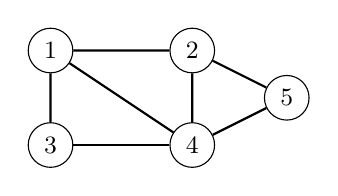
\begin{tikzpicture}[scale=0.6]
\small
\node[draw, circle] (1) at (1,3) {$1$};
\node[draw, circle] (2) at (4,3) {$2$};
\node[draw, circle] (3) at (1,1) {$3$};
\node[draw, circle] (4) at (4,1) {$4$};
\node[draw, circle] (5) at (6,2) {$5$};

\path[draw,thick,-] (1) -- (2);
\path[draw,thick,-] (1) -- (3);
\path[draw,thick,-] (1) -- (4);
\path[draw,thick,-] (3) -- (4);
\path[draw,thick,-] (2) -- (4);
\path[draw,thick,-] (2) -- (5);
\path[draw,thick,-] (4) -- (5);
\end{tikzpicture}
\end{center}
\caption{Verkko, jossa on viisi solmua ja seitsemän kaarta.}
\label{fig:veresi}
\end{figure}

Sanomme, että kaksi solmua ovat \emph{vierekkäin} verkossa,
jos niiden välillä on kaari.
Solmun \emph{naapureja} ovat kaikki solmut,
joihin se on yhteydessä kaarella,
ja solmun \emph{aste} on sen naapureiden määrä.
Kuvassa \ref{fig:veresi} solmun 2 naapurit ovat 1, 4 ja 5,
joten solmun aste on 3.
Voimme kulkea solmusta 1 solmuun 5
esimerkiksi polkua $1 \rightarrow 2 \rightarrow 5$
tai $1 \rightarrow 3 \rightarrow 4 \rightarrow 5$.

\subsubsection{Polku ja sykli}

\begin{figure}
\center
\begin{center}
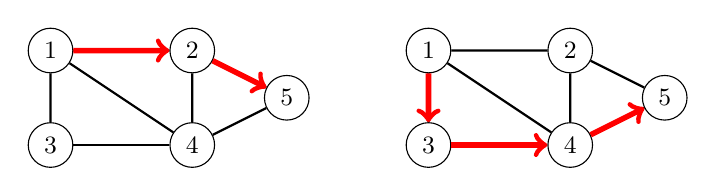
\begin{tikzpicture}[scale=0.6]
\small
\begin{scope}
\node[draw, circle] (1) at (1,3) {$1$};
\node[draw, circle] (2) at (4,3) {$2$};
\node[draw, circle] (3) at (1,1) {$3$};
\node[draw, circle] (4) at (4,1) {$4$};
\node[draw, circle] (5) at (6,2) {$5$};

\path[draw,thick,-] (1) -- (2);
\path[draw,thick,-] (1) -- (3);
\path[draw,thick,-] (1) -- (4);
\path[draw,thick,-] (3) -- (4);
\path[draw,thick,-] (2) -- (4);
\path[draw,thick,-] (2) -- (5);
\path[draw,thick,-] (4) -- (5);

\path[draw,thick,->,red,line width=2pt] (1) -- (2);
\path[draw,thick,->,red,line width=2pt] (2) -- (5);
\end{scope}
\begin{scope}[xshift=8cm]
\node[draw, circle] (1) at (1,3) {$1$};
\node[draw, circle] (2) at (4,3) {$2$};
\node[draw, circle] (3) at (1,1) {$3$};
\node[draw, circle] (4) at (4,1) {$4$};
\node[draw, circle] (5) at (6,2) {$5$};

\path[draw,thick,-] (1) -- (2);
\path[draw,thick,-] (1) -- (3);
\path[draw,thick,-] (1) -- (4);
\path[draw,thick,-] (3) -- (4);
\path[draw,thick,-] (2) -- (4);
\path[draw,thick,-] (2) -- (5);
\path[draw,thick,-] (4) -- (5);

\path[draw,thick,->,red,line width=2pt] (1) -- (3);
\path[draw,thick,->,red,line width=2pt] (3) -- (4);
\path[draw,thick,->,red,line width=2pt] (4) -- (5);
\end{scope}
\end{tikzpicture}
\end{center}
\caption{Kaksi polkua solmusta $1$ solmuun $5$.}
\label{fig:verpoe}
\end{figure}

Verkossa oleva \emph{polku} on kaaria pitkin kulkeva reitti
lähtösolmusta kohdesolmuun.
Kuva \ref{fig:verpoe} näyttää kaksi
mahdollista polkua solmusta $1$ solmuun $5$ esimerkkiverkossamme.
Ensimmäinen polku on $1 \rightarrow 2 \rightarrow 5$
ja toinen polku on $1 \rightarrow 3 \rightarrow 4 \rightarrow 5$.

\begin{figure}
\center
\begin{center}
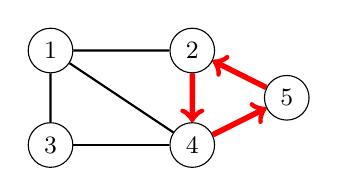
\begin{tikzpicture}[scale=0.6]
\small
\node[draw, circle] (1) at (1,3) {$1$};
\node[draw, circle] (2) at (4,3) {$2$};
\node[draw, circle] (3) at (1,1) {$3$};
\node[draw, circle] (4) at (4,1) {$4$};
\node[draw, circle] (5) at (6,2) {$5$};

\path[draw,thick,-] (1) -- (2);
\path[draw,thick,-] (1) -- (3);
\path[draw,thick,-] (1) -- (4);
\path[draw,thick,-] (3) -- (4);
\path[draw,thick,-] (2) -- (4);
\path[draw,thick,-] (2) -- (5);
\path[draw,thick,-] (4) -- (5);

\path[draw,thick,->,red,line width=2pt] (2) -- (4);
\path[draw,thick,->,red,line width=2pt] (4) -- (5);
\path[draw,thick,->,red,line width=2pt] (5) -- (2);
\end{tikzpicture}
\end{center}
\caption{Verkossa on sykli $2 \rightarrow 4 \rightarrow 5 \rightarrow 2$.}
\label{fig:versyk}
\end{figure}


Polku on \emph{sykli},
jos se alkaa ja päättyy samassa solmussa,
kulkee ainakin yhden toisen solmun kautta
eikä kulje kahta kertaa saman solmun tai kaaren kautta.
Kuvassa \ref{fig:versyk} on esimerkkinä sykli
$2 \rightarrow 4 \rightarrow 5 \rightarrow 2$.
Jos verkossa ei ole yhtään sykliä, sanomme, että verkko on \emph{syklitön}.

\subsubsection{Yhtenäisyys ja komponentit}

Verkko on \emph{yhtenäinen},
jos minkä tahansa kahden solmun välillä on polku.
Kuvan \ref{fig:veresi} verkko on yhtenäinen,
mutta kuvan \ref{fig:veryht} verkko ei ole yhtenäinen,
koska esimerkiksi solmujen $1$ ja $2$ välillä ei ole polkua.

Voimme esittää verkon aina kokoelmana yhtenäisiä \emph{komponentteja}.
Kuvassa \ref{fig:veryht} yhtenäiset komponentit
ovat $\{1,3\}$ ja $\{2,4,5\}$.

\begin{figure}
\center
\begin{center}
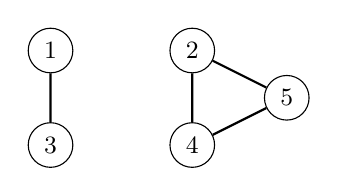
\begin{tikzpicture}[scale=0.6]
\small
\node[draw, circle] (1) at (1,3) {$1$};
\node[draw, circle] (2) at (4,3) {$2$};
\node[draw, circle] (3) at (1,1) {$3$};
\node[draw, circle] (4) at (4,1) {$4$};
\node[draw, circle] (5) at (6,2) {$5$};

\path[draw,thick,-] (1) -- (3);
\path[draw,thick,-] (2) -- (4);
\path[draw,thick,-] (2) -- (5);
\path[draw,thick,-] (4) -- (5);
\end{tikzpicture}
\end{center}
\caption{Verkon yhtenäiset komponentit ovat $\{1,3\}$ ja $\{2,4,5\}$.}
\label{fig:veryht}
\end{figure}

Verkko on \emph{puu}, jos se on sekä yhtenäinen
että syklitön.
Puussa kaarten määrä on aina yhden pienempi
kuin solmujen määrä, ja jokaisen kahden solmun
välillä on yksikäsitteinen polku.
Kuvassa \ref{fig:verpuu} on esimerkkinä puu,
jossa on viisi solmua ja neljä kaarta.

\begin{figure}
\center
\begin{center}
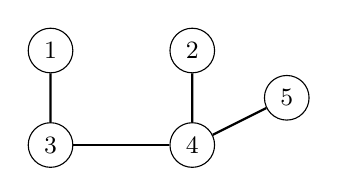
\begin{tikzpicture}[scale=0.6]
\small
\node[draw, circle] (1) at (1,3) {$1$};
\node[draw, circle] (2) at (4,3) {$2$};
\node[draw, circle] (3) at (1,1) {$3$};
\node[draw, circle] (4) at (4,1) {$4$};
\node[draw, circle] (5) at (6,2) {$5$};

\path[draw,thick,-] (1) -- (3);
\path[draw,thick,-] (3) -- (4);
\path[draw,thick,-] (2) -- (4);
\path[draw,thick,-] (4) -- (5);
\end{tikzpicture}
\end{center}
\caption{Yhtenäinen, syklitön verkko eli puu.}
\label{fig:verpuu}
\end{figure}

\subsubsection{Suunnattu verkko}

\emph{Suunnatussa} verkossa
jokaisella kaarella on tietty suunta,
jonka mukaisesti meidän täytyy kulkea kaarta pitkin.
Suunnat rajoittavat siis kulkemistamme verkossa.
Kuvassa \ref{fig:versuu} on esimerkkinä
suunnattu verkko, jossa
voimme kulkea solmusta $1$ solmuun $5$
polkua $1 \rightarrow 2 \rightarrow 5$,
mutta emme voi kulkea mitenkään solmusta $5$ solmuun $1$.

\begin{figure}
\center
\begin{center}
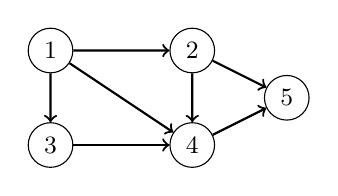
\begin{tikzpicture}[scale=0.6]
\small
\node[draw, circle] (1) at (1,3) {$1$};
\node[draw, circle] (2) at (4,3) {$2$};
\node[draw, circle] (3) at (1,1) {$3$};
\node[draw, circle] (4) at (4,1) {$4$};
\node[draw, circle] (5) at (6,2) {$5$};

\path[draw,thick,->] (1) -- (2);
\path[draw,thick,->] (1) -- (3);
\path[draw,thick,->] (1) -- (4);
\path[draw,thick,->] (3) -- (4);
\path[draw,thick,->] (2) -- (4);
\path[draw,thick,->] (2) -- (5);
\path[draw,thick,->] (4) -- (5);
\end{tikzpicture}
\end{center}
\caption{Suunnattu verkko.}
\label{fig:versuu}
\end{figure}

\subsubsection{Painotettu verkko}

\emph{Painotetussa} verkossa
jokaiseen kaareen liittyy jokin paino,
joka kuvaa tyypillisesti kaaren pituutta.
Kun kuljemme polkua painotetussa verkossa,
polun pituus on kaarten painojen summa.
Kuvassa \ref{fig:verpae} on esimerkkinä painotettu verkko.
Tässä verkossa polun $1 \rightarrow 2 \rightarrow 5$
paino on $5+8=13$ ja polun
$1 \rightarrow 3 \rightarrow 4 \rightarrow 5$
paino on $2+4+3=9$.

\begin{figure}
\center
\begin{center}
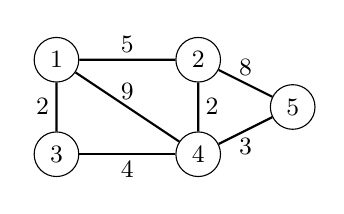
\begin{tikzpicture}[scale=0.6,label distance=-1.5mm]
\small
\node[draw, circle] (1) at (1,3) {$1$};
\node[draw, circle] (2) at (4,3) {$2$};
\node[draw, circle] (3) at (1,1) {$3$};
\node[draw, circle] (4) at (4,1) {$4$};
\node[draw, circle] (5) at (6,2) {$5$};

\path[draw,thick,-] (1) -- node[font=\small,label=above:5] {} (2);
\path[draw,thick,-] (1) -- node[font=\small,label=left:2] {} (3);
\path[draw,thick,-] (1) -- node[font=\small,label=above:9] {} (4);
\path[draw,thick,-] (3) -- node[font=\small,label=below:4] {} (4);
\path[draw,thick,-] (2) -- node[font=\small,label=above:8] {} (5);
\path[draw,thick,-] (4) -- node[font=\small,label=right:2] {} (2);
\path[draw,thick,-] (4) -- node[font=\small,label=below:3] {} (5);
\end{tikzpicture}
\end{center}
\caption{Painotettu verkko.}
\label{fig:verpae}
\end{figure}


\section{Verkot ohjelmoinnissa}

Verkon esittämiseen ohjelmoinnissa on monia mahdollisuuksia.
Sopivan esitystavan valintaan vaikuttaa,
miten haluamme käsitellä verkkoa algoritmissa,
koska jokaisessa esitystavassa on omat etunsa.
Seuraavaksi käymme läpi kolme tavallista esitystapaa.

\subsection{Vieruslistaesitys}

\begin{figure}
\center
\begin{center}
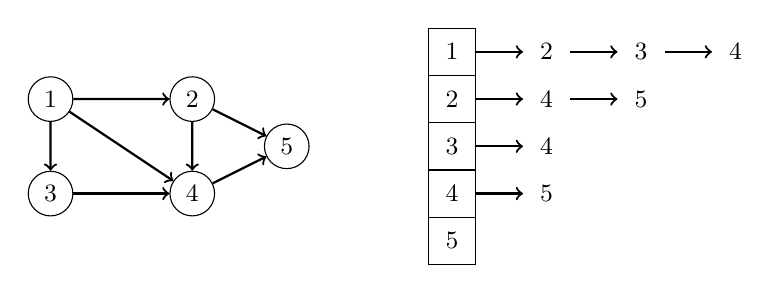
\begin{tikzpicture}[scale=0.6]
\small
\begin{scope}
\node[draw, circle] (1) at (1,3) {$1$};
\node[draw, circle] (2) at (4,3) {$2$};
\node[draw, circle] (3) at (1,1) {$3$};
\node[draw, circle] (4) at (4,1) {$4$};
\node[draw, circle] (5) at (6,2) {$5$};

\path[draw,thick,->] (1) -- (2);
\path[draw,thick,->] (1) -- (3);
\path[draw,thick,->] (1) -- (4);
\path[draw,thick,->] (3) -- (4);
\path[draw,thick,->] (2) -- (4);
\path[draw,thick,->] (2) -- (5);
\path[draw,thick,->] (4) -- (5);
\end{scope}
\begin{scope}[xshift=9cm,yshift=-0.5cm]
\draw (0,0) grid (1,5);
\foreach \x in {1,...,5} \node at (0.5,0.5-\x+5) {\x};
\draw[->,thick] (1,4.5) -- (2,4.5);
\draw[->,thick] (3,4.5) -- (4,4.5);
\draw[->,thick] (5,4.5) -- (6,4.5);
\draw[->,thick] (1,3.5) -- (2,3.5);
\draw[->,thick] (3,3.5) -- (4,3.5);
\draw[->,thick] (1,2.5) -- (2,2.5);
\draw[->,thick] (1,1.5) -- (2,1.5);
\node at (2.5,4.5) {$2$};
\node at (4.5,4.5) {$3$};
\node at (6.5,4.5) {$4$};
\node at (2.5,3.5) {$4$};
\node at (4.5,3.5) {$5$};
\node at (2.5,2.5) {$4$};
\node at (2.5,1.5) {$5$};
\end{scope}
\end{tikzpicture}
\end{center}
\caption{Verkon vieruslistaesitys.}
\label{fig:vervil}
\end{figure}

Vieruslistaesityksessä luomme kullekin verkon solmulle
\emph{vieruslistan}, joka kertoo, mihin solmuihin voimme
siirtyä solmusta kaaria pitkin.
Kuva \ref{fig:vervil} näyt\-tää esimerkkinä verkon
ja sitä vastaavan vieruslistaesityksen.
Jos haluamme tallentaa verkon vieruslistoina Javassa,
voimme luoda taulukon

\begin{code}
ArrayList<Integer>[] verkko = new ArrayList<>[n+1];
\end{code}

ja alustaa vieruslistat näin:

\begin{code}
for (int i = 1; i <= n; i++) {
    verkko[i] = new ArrayList<>();
}
\end{code}

Tämän jälkeen lisäämme kaaret listoille näin:

\begin{code}
verkko[1].add(2);
verkko[1].add(3);
verkko[1].add(4);
verkko[2].add(4);
verkko[2].add(5);
verkko[3].add(4);
verkko[4].add(5);
\end{code}

Vieruslistaesitys on monessa tilanteessa hyvä tapa tallentaa verkko,
koska haluamme usein selvittää,
mihin solmuihin pääsemme siirtymään tietystä solmusta kaaria pitkin.
Esimerkiksi seuraava koodi käy läpi solmut,
joihin voimme siirtyä solmusta $x$ kaarella:

\begin{code}
for (Integer s : verkko[x]) {
    // käsittele solmu s
}
\end{code}

\subsection{Kaarilistaesitys}

Kaarilistaesityksessä luomme listan,
jossa on kaikki verkon kaaret.
Javassa voimme luoda listan

\begin{code}
ArrayList<Kaari> kaaret = new ArrayList<>();
\end{code}

jossa on seuraavanlaisia kaaria:

\begin{code}
public class Kaari {
    public int alku, loppu;

    public Kaari(int alku, int loppu) {
        this.alku = alku;
        this.loppu = loppu;
    }
}
\end{code}

Seuraava koodi luo esimerkkiverkkoamme vastaavan kaarilistan:

\begin{code}
kaaret.add(new Kaari(1,2));
kaaret.add(new Kaari(1,3));
kaaret.add(new Kaari(1,4));
kaaret.add(new Kaari(2,4));
kaaret.add(new Kaari(2,5));
kaaret.add(new Kaari(3,4));
kaaret.add(new Kaari(4,5));
\end{code}

Kaarilista on hyvä esitystapa algoritmeissa,
joissa meidän täytyy pystyä käymään helposti läpi
kaikki verkon kaaret eikä meillä ole tarvetta
selvittää tietystä solmusta lähteviä kaaria.

\subsection{Vierusmatriisiesitys}

\begin{figure}
\center
\begin{center}
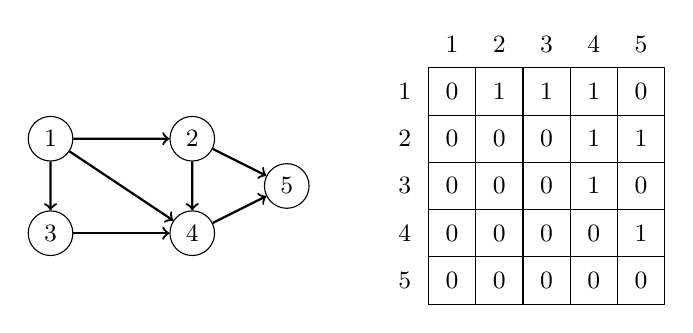
\begin{tikzpicture}[scale=0.6]
\small
\begin{scope}
\node[draw, circle] (1) at (1,3) {$1$};
\node[draw, circle] (2) at (4,3) {$2$};
\node[draw, circle] (3) at (1,1) {$3$};
\node[draw, circle] (4) at (4,1) {$4$};
\node[draw, circle] (5) at (6,2) {$5$};

\path[draw,thick,->] (1) -- (2);
\path[draw,thick,->] (1) -- (3);
\path[draw,thick,->] (1) -- (4);
\path[draw,thick,->] (3) -- (4);
\path[draw,thick,->] (2) -- (4);
\path[draw,thick,->] (2) -- (5);
\path[draw,thick,->] (4) -- (5);
\end{scope}
\begin{scope}[xshift=9cm,yshift=-0.5cm]
\draw (0,0) grid (5,5);
\foreach \x in {1,...,5} \node at (-0.5,0.5-\x+5) {\x};
\foreach \x in {1,...,5} \node at (-0.5+\x,5.5) {\x};
\foreach \x/\v in {1/0,2/1,3/1,4/1,5/0} \node at (-0.5+\x,4.5) {\v};
\foreach \x/\v in {1/0,2/0,3/0,4/1,5/1} \node at (-0.5+\x,3.5) {\v};
\foreach \x/\v in {1/0,2/0,3/0,4/1,5/0} \node at (-0.5+\x,2.5) {\v};
\foreach \x/\v in {1/0,2/0,3/0,4/0,5/1} \node at (-0.5+\x,1.5) {\v};
\foreach \x/\v in {1/0,2/0,3/0,4/0,5/0} \node at (-0.5+\x,0.5) {\v};
\end{scope}
\end{tikzpicture}
\end{center}
\caption{Verkon vierusmatriisiesitys.}
\label{fig:vervim}
\end{figure}

Vierusmatriisi on kaksiulotteinen taulukko,
joka kertoo jokaisesta verkon kaaresta,
esiintyykö se verkossa.
Jos verkossa pääsee kaarella solmusta
$a$ solmuun $b$,
niin matriisin rivin $a$ sarakkeessa $b$
on sitä vastaava merkintä.
Kuvassa \ref{fig:vervim} on esimerkki
verkon vierusmatriisiesityksestä.

Javassa voimme määritellä vierusmatriisin seuraavasti:

\begin{code}
int[][] verkko = new int[n+1][n+1];
\end{code}

Tämän jälkeen merkitsemme, miten voimme kulkea
solmujen välillä kaaria pitkin:

\begin{code}
verkko[1][2] = 1;
verkko[1][3] = 1;
verkko[1][4] = 1;
verkko[2][4] = 1;
verkko[2][5] = 1;
verkko[3][4] = 1;
verkko[4][5] = 1;
\end{code}

Vierusmatriisin etuna on, että voimme tarkastaa helposti,
onko tietty kaari verkossa.
Esitystapa kuluttaa kuitenkin paljon muistia,
eikä sitä voi käyttää, jos verkon solmujen määrä on suuri.

\section{Syvyyshaku}

\emph{Syvyyshaku} on verkkojen käsittelyn perusalgoritmi,
joka etsii kaikki solmut, jotka ovat saavutettavissa
annetusta lähtösolmusta.
Voimme selvittää syvyyshaun avulla monia asioita
verkon rakenteesta.

Syvyyshaku lähtee liikkeelle tietystä verkon solmusta
ja alkaa tutkia verkkoa siitä käsin.
Algoritmi pitää yllä jokaisesta solmusta tietoa,
onko se vielä vieraillut solmussa.
Kun haku saapuu solmuun, jossa se ei ole käynyt aiemmin,
se merkitsee solmun vierailluksi ja
etenee syvemmälle verkossa jatkamalla hakua
yksi kerrallaan solmusta lähteviä kaaria pitkin.
Tämän jälkeen algoritmi perääntyy taaksepäin
samaa polkua kuin tuli solmuun.

\begin{figure}
\center
\begin{center}
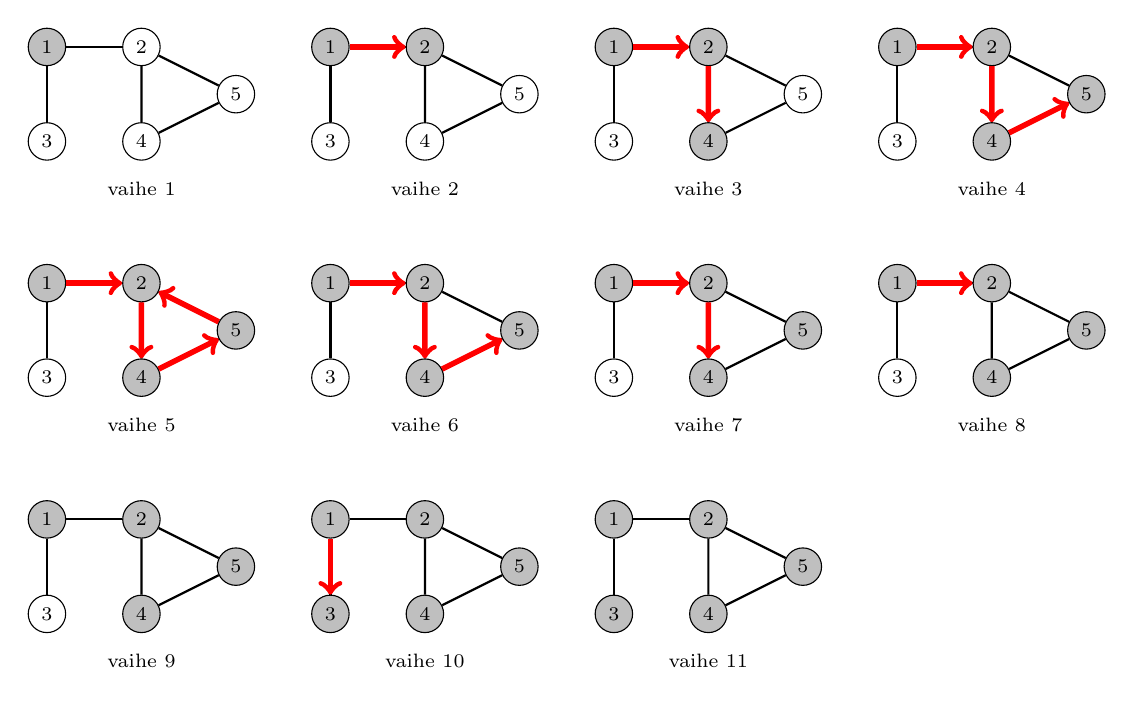
\begin{tikzpicture}[scale=0.6]
\scriptsize
\newcommand\verkko[6]{
\node[draw, circle, fill=#2] (1) at (0,0) {$1$};
\node[draw, circle, fill=#3] (2) at (2,0) {$2$};
\node[draw, circle, fill=#4] (3) at (0,-2) {$3$};
\node[draw, circle, fill=#5] (4) at (2,-2) {$4$};
\node[draw, circle, fill=#6] (5) at (4,-1) {$5$};
\path[draw,thick,-] (1) -- (2);
\path[draw,thick,-] (2) -- (5);
\path[draw,thick,-] (2) -- (4);
\path[draw,thick,-] (4) -- (5);
\path[draw,thick,-] (1) -- (3);
\node at (2,-3) {vaihe #1};
}
\begin{scope}
\verkko{1}{lightgray}{white}{white}{white}{white}
\end{scope}
\begin{scope}[xshift=6cm]
\verkko{2}{lightgray}{lightgray}{white}{white}{white}
\path[draw=red,thick,->,line width=2pt] (1) -- (2);
\end{scope}
\begin{scope}[xshift=12cm]
\verkko{3}{lightgray}{lightgray}{white}{lightgray}{white}
\path[draw=red,thick,->,line width=2pt] (1) -- (2);
\path[draw=red,thick,->,line width=2pt] (2) -- (4);
\end{scope}
\begin{scope}[xshift=18cm]
\verkko{4}{lightgray}{lightgray}{white}{lightgray}{lightgray}
\path[draw=red,thick,->,line width=2pt] (1) -- (2);
\path[draw=red,thick,->,line width=2pt] (2) -- (4);
\path[draw=red,thick,->,line width=2pt] (4) -- (5);
\end{scope}
\begin{scope}[yshift=-5cm]
\verkko{5}{lightgray}{lightgray}{white}{lightgray}{lightgray}
\path[draw=red,thick,->,line width=2pt] (1) -- (2);
\path[draw=red,thick,->,line width=2pt] (2) -- (4);
\path[draw=red,thick,->,line width=2pt] (4) -- (5);
\path[draw=red,thick,->,line width=2pt] (5) -- (2);
\end{scope}
\begin{scope}[yshift=-5cm,xshift=6cm]
\verkko{6}{lightgray}{lightgray}{white}{lightgray}{lightgray}
\path[draw=red,thick,->,line width=2pt] (1) -- (2);
\path[draw=red,thick,->,line width=2pt] (2) -- (4);
\path[draw=red,thick,->,line width=2pt] (4) -- (5);
\end{scope}
\begin{scope}[yshift=-5cm,xshift=12cm]
\verkko{7}{lightgray}{lightgray}{white}{lightgray}{lightgray}
\path[draw=red,thick,->,line width=2pt] (1) -- (2);
\path[draw=red,thick,->,line width=2pt] (2) -- (4);
\end{scope}
\begin{scope}[yshift=-5cm,xshift=18cm]
\verkko{8}{lightgray}{lightgray}{white}{lightgray}{lightgray}
\path[draw=red,thick,->,line width=2pt] (1) -- (2);
\end{scope}
\begin{scope}[yshift=-10cm]
\verkko{9}{lightgray}{lightgray}{white}{lightgray}{lightgray}
\end{scope}
\begin{scope}[yshift=-10cm,xshift=6cm]
\verkko{10}{lightgray}{lightgray}{lightgray}{lightgray}{lightgray}
\path[draw=red,thick,->,line width=2pt] (1) -- (3);
\end{scope}
\begin{scope}[yshift=-10cm,xshift=12cm]
\verkko{11}{lightgray}{lightgray}{lightgray}{lightgray}{lightgray}
\end{scope}
\end{tikzpicture}
\end{center}
\caption{Esimerkki syvyyshaun toiminnasta.}
\label{fig:syvhak}
\end{figure}

Kuvassa \ref{fig:syvhak} on esimerkki syvyyshaun toiminnasta.
Jokaisessa vaiheessa harmaat solmut ovat solmuja,
joissa haku on jo vieraillut.
Haku lähtee liikkeelle solmusta 1,
josta pääsee solmuihin 2 ja 3.
Haku etenee ensin solmuun 2, josta pääsee edelleen
solmuihin 4 ja 5.
Koska haku ei enää pysty etenemään solmusta 5,
se perääntyy takaisin solmuun 1.
Tämän jälkeen haku käy vielä solmussa 3,
minkä jälkeen se on käynyt läpi kaikki solmut,
joihin pääsee solmusta 1.

\subsection{Algoritmin toteutus}

Syvyyshaku on mukavaa toteuttaa rekursiivisesti.
Tarvitsemme ensinnäkin taulukon, joka kertoo,
missä solmuissa olemme käyneet:

\begin{code}
boolean[] vierailtu = new boolean[n+1];
\end{code}

Tämän jälkeen voimme toteuttaa syvyyshaun näin
käyttäen verkon vieruslistaesitystä:

\begin{code}
void syvyyshaku(int solmu) {
    if (vierailtu[solmu]) return;
    vierailtu[solmu] = true;
    for (Integer naapuri : verkko[solmu]) {
        syvyyshaku(naapuri);
    }
}
\end{code}

Syvyyshaku käynnistyy, kun kutsumme metodia
\texttt{syvyyshaku} parametrina lähtösolmu.
Jokaisella kutsulla metodi tarkistaa ensin,
olemmeko jo käyneet parametrina annetussa solmussa,
ja päättyy heti tässä tilanteessa.
Muuten metodi merkitsee, että olemme nyt käyneet solmussa
ja etenee rekursiivisesti kaikkiin solmun naapureihin.

Syvyyshaku käsittelee kerran jokaisen solmun,
johon pääsee lähtösolmusta,
käymällä läpi siitä lähtevät kaaret.
Niinpä syvyyshaku vie aikaa $O(n+m)$, missä $n$ on
verkon solmujen määrä ja $m$ on verkon kaarten määrä.

\subsection{Sovelluksia}

Syvyyshaku on yleistyökalu verkko-ongelmien ratkaisemiseen.
Seuraavassa on joitakin esimerkkejä syvyyshaun käyttökohteista.
Oletamme, että verkko on suuntaamaton, eli voimme kulkea
kaikkia kaaria kumpaankin suuntaan.

\subsubsection{Polun etsiminen}

Syvyyshaun avulla voimme etsiä verkosta polun solmusta
$a$ solmuun $b$, jos tällainen polku on olemassa.
Tämä tapahtuu aloittamalla haku solmusta $a$
ja pysähtymällä, kun vastaan tulee solmu $b$.
Jos polkuja on useita, syvyyshaku löytää jonkin niistä
riippuen solmujen käsittelyjärjestyksestä.

\subsubsection{Yhtenäisyys ja komponentit}

Verkko on yhtenäinen, jos kaikki solmut ovat yhteydessä
toisiinsa.
Voimmekin tarkastaa verkon yhtenäisyyden aloittamalla
syvyyshaun mielivaltaisesta solmusta ja tutkimalla,
saavuttaako haku kaikki verkon solmut.
Lisäksi voimme löytää verkon yhtenäiset komponentit
käymällä läpi solmut ja aloittamalla syvyyshaun aina,
kun vastaan tulee uusi solmu.
Jokainen syvyyshaku muodostaa yhden komponentin.

\subsubsection{Syklin etsiminen}

Jos verkossa on sykli, huomaamme sen syvyyshaun aikana siitä,
että tulemme tulemme toista kautta johonkin solmuun,
jossa olemme käyneet jo aiemmin.
Niinpä löydämme syvyyshaun avulla jonkin verkossa olevan
syklin, jos sellainen on olemassa.

\section{Leveyshaku}

\emph{Leveyshaku} on algoritmi, joka selvittää \emph{lyhimmän} polun
lähtösolmusta kaikkiin solmuihin, jotka ovat saavutettavissa siitä.
Lyhin polku tarkoittaa tässä polkua, jossa on mahdollisimman vähän kaaria.
Ideana on käsitellä solmut kerroksittain lähtösolmusta alkaen
siinä järjestyksessä kuin olemme löytäneet ne.
Jokaisen solmun kohdalla käymme läpi kaikki siitä lähtevät kaaret.

\begin{figure}
\center
\begin{center}
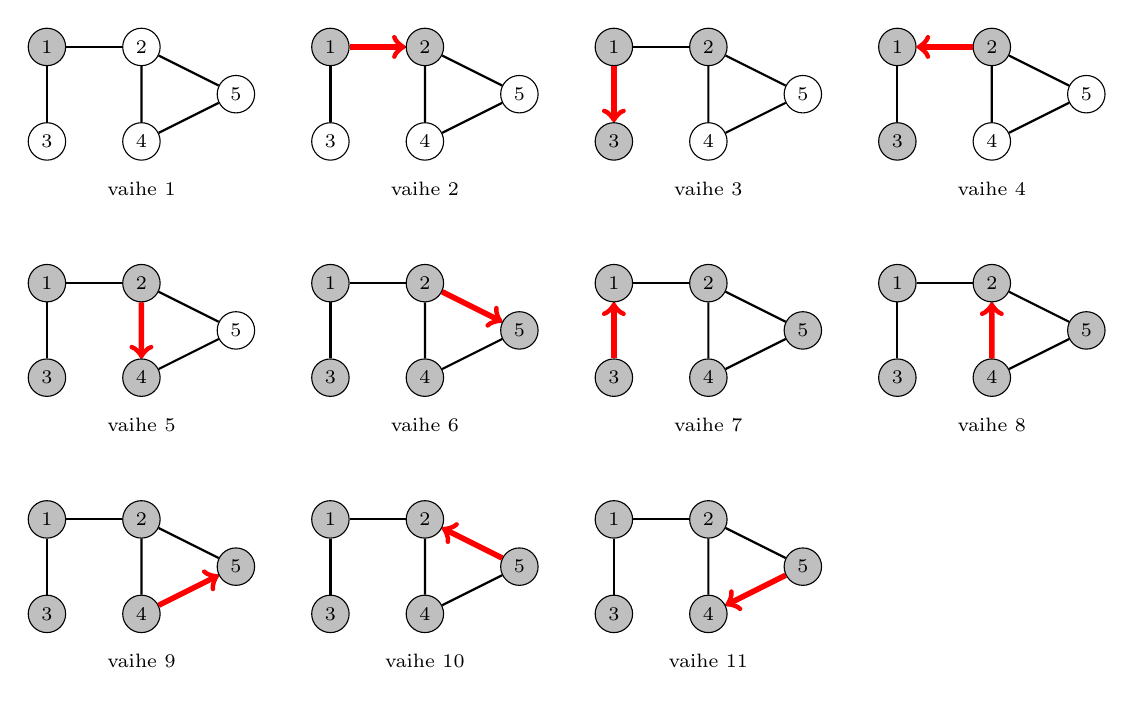
\begin{tikzpicture}[scale=0.6]
\scriptsize
\newcommand\verkko[6]{
\node[draw, circle, fill=#2] (1) at (0,0) {$1$};
\node[draw, circle, fill=#3] (2) at (2,0) {$2$};
\node[draw, circle, fill=#4] (3) at (0,-2) {$3$};
\node[draw, circle, fill=#5] (4) at (2,-2) {$4$};
\node[draw, circle, fill=#6] (5) at (4,-1) {$5$};
\path[draw,thick,-] (1) -- (2);
\path[draw,thick,-] (2) -- (5);
\path[draw,thick,-] (2) -- (4);
\path[draw,thick,-] (4) -- (5);
\path[draw,thick,-] (1) -- (3);
\node at (2,-3) {vaihe #1};
}
\begin{scope}
\verkko{1}{lightgray}{white}{white}{white}{white}
\end{scope}
\begin{scope}[xshift=6cm]
\verkko{2}{lightgray}{lightgray}{white}{white}{white}
\path[draw=red,thick,->,line width=2pt] (1) -- (2);
\end{scope}
\begin{scope}[xshift=12cm]
\verkko{3}{lightgray}{lightgray}{lightgray}{white}{white}
\path[draw=red,thick,->,line width=2pt] (1) -- (3);
\end{scope}
\begin{scope}[xshift=18cm]
\verkko{4}{lightgray}{lightgray}{lightgray}{white}{white}
\path[draw=red,thick,->,line width=2pt] (2) -- (1);
\end{scope}
\begin{scope}[yshift=-5cm,xshift=0cm]
\verkko{5}{lightgray}{lightgray}{lightgray}{lightgray}{white}
\path[draw=red,thick,->,line width=2pt] (2) -- (4);
\end{scope}
\begin{scope}[yshift=-5cm,xshift=6cm]
\verkko{6}{lightgray}{lightgray}{lightgray}{lightgray}{lightgray}
\path[draw=red,thick,->,line width=2pt] (2) -- (5);
\end{scope}
\begin{scope}[yshift=-5cm,xshift=12cm]
\verkko{7}{lightgray}{lightgray}{lightgray}{lightgray}{lightgray}
\path[draw=red,thick,->,line width=2pt] (3) -- (1);
\end{scope}
\begin{scope}[yshift=-5cm,xshift=18cm]
\verkko{8}{lightgray}{lightgray}{lightgray}{lightgray}{lightgray}
\path[draw=red,thick,->,line width=2pt] (4) -- (2);
\end{scope}
\begin{scope}[yshift=-10cm,xshift=0cm]
\verkko{9}{lightgray}{lightgray}{lightgray}{lightgray}{lightgray}
\path[draw=red,thick,->,line width=2pt] (4) -- (5);
\end{scope}
\begin{scope}[yshift=-10cm,xshift=6cm]
\verkko{10}{lightgray}{lightgray}{lightgray}{lightgray}{lightgray}
\path[draw=red,thick,->,line width=2pt] (5) -- (2);
\end{scope}
\begin{scope}[yshift=-10cm,xshift=12cm]
\verkko{11}{lightgray}{lightgray}{lightgray}{lightgray}{lightgray}
\path[draw=red,thick,->,line width=2pt] (5) -- (4);
\end{scope}
\end{tikzpicture}
\end{center}
\caption{Esimerkki leveyshaun toiminnasta.}
\label{fig:levhak}
\end{figure}

Kuvassa \ref{fig:levhak} on esimerkki leveyshaun toiminnasta,
kun etsimme polkuja solmusta 1 aloittaen.
Käsittelemme ensin solmun 1, josta pääsemme uusiin solmuihin 2 ja 3.
Tämä tarkoittaa, että lyhimmät polut solmuihin 2 ja 3
ovat $1 \rightarrow 2$ ja $1 \rightarrow 3$.
Sitten käsittelemme solmun 2, josta pääsemme uusiin solmuihin 4 ja 5.
Tämä tarkoittaa, että lyhimmät polut solmuihin 4 ja 5
ovat $1 \rightarrow 2 \rightarrow 4$ ja $1 \rightarrow 2 \rightarrow 5$.
Lopuksi käsittelemme vielä solmut 3, 4 ja 5,
joista emme kuitenkaan pääse enää uusiin solmuihin.

\subsection{Algoritmin toteutus}

Leveyshaku on vaikeampi toteuttaa kuin syvyyshaku,
koska meidän täytyy pystyä edistämään hakua vuorotellen verkon eri puolilta.
Tätä varten luomme \emph{jonon}, joka sisältää läpikäyntiä odottavia solmuja.
Valitsemme aina seuraavaksi käsiteltävän solmun jonon alusta,
ja lisämme uudet vieraillut solmut jonon loppuun.
Voimme luoda jonon näin:

\begin{code}
ArrayDeque<Integer> jono = new ArrayDeque<>();
\end{code}

Lisäksi määrittelemme syvyyshaun tapaan taulukon, jossa pidämme kirjaa,
missä solmuissa olemme käyneet:

\begin{code}
boolean[] vierailtu = new boolean[n+1];
\end{code}

Oletamme seuraavassa koodissa, että aloitamme leveyshaun solmusta \texttt{alku} alkaen.
Voimme toteuttaa haun seuraavasti:

\begin{code}
vierailtu[alku] = true;
jono.addLast(alku);
while (jono.size() > 0) {
    int solmu = jono.pollFirst();
    for (int naapuri : verkko[solmu]) {
        if (vierailtu[naapuri]) continue;
        vierailtu[naapuri] = true;
        jono.addLast(naapuri);
    }
}
\end{code}

Koodi merkitsee aluksi, että olemme käyneet lähtösolmussa
sekä lisää lähtösolmun jonoon.
Tämän jälkeen joka askeleella haku valitsee
jonon ensimmäisen solmun ja tarkastaa siitä lähtevät kaaret.
Jos pääsemme uuteen solmuun, merkitsemme uuden solmun
vierailluksi ja lisäämme sen jonoon.
Haku jatkuu niin kauan kuin jonossa on solmuja.

Syvyyshaun tavoin leveyshaku vie aikaa $O(n+m)$,
koska käymme läpi kerran jokaisesta solmusta lähtevät kaaret.

\subsection{Polkujen etsiminen}

Vaikka leveyshakua voi käyttää yleisalgoritmina verkon läpikäyntiin,
yleensä tavoitteena on nimenomaan löytää lyhimmät polut lähtösolmusta
muihin solmuihin. Tätä varten määrittelemme kaksi uutta taulukkoa:

\begin{code}
int[] etaisyys = new int[n+1];
int[] aiempi = new int[n+1];
\end{code}

Taulukko \texttt{etaisyys} kertoo, mikä on etäisyys
(eli lyhimmän polun pituus) lähtösolmusta kyseiseen solmuun,
ja taulukko \texttt{aiempi} viittaa edelliseen solmuun lyhimmällä polulla.
Näiden taulukoiden avulla voimme leveyshaun jälkeen muodostaa
lyhimmän polun lähtösolmusta mihin tahansa solmuun.
Päivitäm\-me taulukoita seuraavasti haun aikana:

\begin{code}
vierailtu[alku] = true;
etaisyys[alku] = 0;
aiempi[alku] = 0;
jono.addLast(alku);
while (jono.size() > 0) {
    int solmu = jono.pollFirst();
    for (int naapuri : verkko[solmu]) {
        if (vierailtu[naapuri]) continue;
        vierailtu[naapuri] = true;
        etaisyys[naapuri] = etaisyys[solmu]+1;
        aiempi[naapuri] = solmu;
        jono.addLast(naapuri);
    }
}
\end{code}

Haun alussa merkitsemme, että etäisyys lähtösolmuun on 0
ja sillä ei ole edellistä solmua.
Sitten kun löydämme uuden solmun, päivitämme sen etäisyyden
ja edellisen solmun polulla.

Nyt leveyshaun jälkeen lyhimmän polun pituus lähtösolmusta
solmuun $x$ on $\texttt{etaisyys}[x]$ ja voimme käydä läpi polulla
olevat solmut seuraavasti (käänteisessä järjestyksessä):

\begin{code}
while (x != 0) {
    System.out.println(x);
    x = aiempi[x];
}
\end{code}

\section{Esimerkki: Labyrintti}

Olemme labyrintissa ja haluamme päästä ruudusta $A$ ruutuun $B$.
Joka askeleella voimme siirtyä yhden ruudun verran ylöspäin, alaspäin,
vasemmalle tai oikealle.
Pystymmekö pääsemään ruudusta $A$ ruutuun $B$, ja jos pystymme, niin
mikä on lyhin mahdollinen reitti?
Esimerkiksi kuvassa \ref{fig:labrei}(a) lyhin reitti
ruudusta $A$ ruutuun $B$ muodostuu 9 askeleesta.

\begin{figure}
\center
\begin{center}
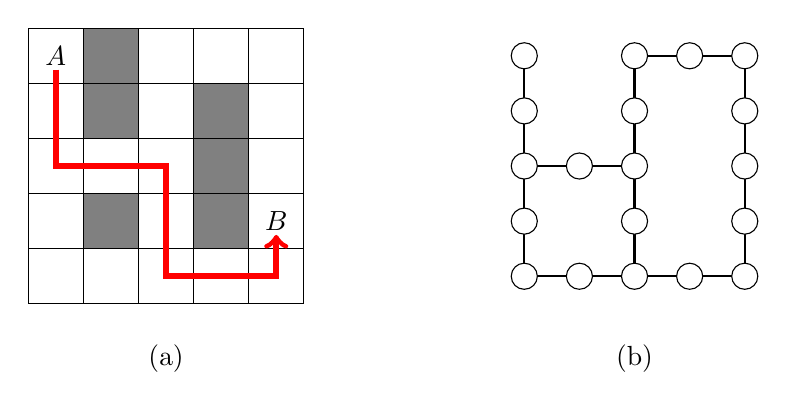
\begin{tikzpicture}[scale=0.7]
\begin{scope}
\draw[fill=gray] (1,1) rectangle (2,2);
\draw[fill=gray] (1,3) rectangle (2,4);
\draw[fill=gray] (1,4) rectangle (2,5);
\draw[fill=gray] (3,1) rectangle (4,2);
\draw[fill=gray] (3,2) rectangle (4,3);
\draw[fill=gray] (3,3) rectangle (4,4);
\draw (0,0) grid (5,5);
\draw[->,thick,red,line width=2pt] (0.5,4.25) -- (0.5,2.5) -- (2.5,2.5) -- (2.5,0.5) -- (4.5,0.5) -- (4.5,1.25);
\node at (0.5,4.5) {$A$};
\node at (4.5,1.5) {$B$};
\node at (2.5,-1) {(a)};
\end{scope}
\begin{scope}[xshift=9cm,yshift=0.5cm]
\foreach \x in {0,1,2,3} \path[draw,thick,-] (0,\x) -- (0,\x+1);
\foreach \x in {0,1,2,3} \path[draw,thick,-] (2,\x) -- (2,\x+1);
\foreach \x in {0,1,2,3} \path[draw,thick,-] (4,\x) -- (4,\x+1);
\foreach \x in {0,1,2,3} \path[draw,thick,-] (\x,0) -- (\x+1,0);
\foreach \x in {0,1} \path[draw,thick,-] (\x,2) -- (\x+1,2);
\foreach \x in {2,3} \path[draw,thick,-] (\x,4) -- (\x+1,4);
\foreach \x in {0,1,2,3,4} \node[draw, circle, fill=white] at (0,\x) {};
\foreach \x in {0,2} \node[draw, circle, fill=white] at (1,\x) {};
\foreach \x in {0,1,2,3,4} \node[draw, circle, fill=white] at (2,\x) {};
\foreach \x in {0,4} \node[draw, circle, fill=white] at (3,\x) {};
\foreach \x in {0,1,2,3,4} \node[draw, circle, fill=white] at (4,\x) {};
\node at (2,-1.5) {(b)};
\end{scope}
\end{tikzpicture}
\end{center}
\caption{(a) Lyhin reitti labyrintissa ruudusta $A$ ruutuun $B$. (b)
Labyrintin esittäminen verkkona.}
\label{fig:labrei}
\end{figure}

Voimme esittää ongelman verkkona niin,
että jokainen labyrintin ruutu on yksi verkon solmuista,
ja kahden solmun välillä on kaari,
jos vastaavat ruudut ovat vierekkäin labyrintissa.
Kuva \ref{fig:labrei}(b) näyttää esimerkkilabyrinttimme verkkona.
Nyt ruudusta $A$ on reitti ruutuun $B$ tarkalleen silloin,
kun vastaavat verkon solmut kuuluvat samaan yhtenäiseen komponenttiin,
minkä voimme tarkastaa syvyyshaulla.
Lyhin reitti ruudusta $A$ ruutuun $B$ löytyy puolestaan leveyshaulla,
joka lähtee liikkeelle ruudusta $A$.

Huomaa, että meidän ei tarvitse erikseen muuttaa labyrinttia
verkoksi, vaan voimme toteuttaa haut \emph{implisiittiseen} verkkoon.
Tämä tarkoittaa, että teemme haun labyrinttiin sen omassa
esitysmuodossa. Käytännössä labyrintti on kätevää tallentaa kaksiulotteisena
taulukkona, joka kertoo, mitkä ruudut ovat seinäruutuja.
Tällöin voimme toteuttaa esimerkiksi syvyyshaun seuraavan tyylisesti:

\begin{code}
void syvyyshaku(int y, int x) {
    if (y < 0 || x < 0 || y >= n || x >= n) return;
    if (seina[y][x] || vierailtu[y][x]) return;
    vierailtu[y][x] = true;
    syvyyshaku(y+1,x);
    syvyyshaku(y-1,x);
    syvyyshaku(y,x+1);
    syvyyshaku(y,x-1);
}
\end{code}
\chapter{Lyhimmät polut}

\index{lyhin polku}
\index{etäisyys}

Monissa verkkoihin liittyvissä ongelmissa on kysymys siitä,
että haluamme löytää \emph{lyhimmän polun} (\emph{shortest path})
verkon solmusta toiseen.
Esimerkiksi voimme haluta selvittää,
mikä on nopein reitti kahden katuosoitteen välillä
tai mikä on halvin tapa lentää kaupungista toiseen.
Näissä ja muissa sovelluksissa on tärkeää,
että löydämme lyhimmän polun tehokkaasti.

Olemme käyttäneet aiemmin leveyshakua lyhimpien
polkujen etsimiseen.
Tämä onkin hyvä ratkaisu, kun haluamme löytää polut,
joiden kaarten määrä on pienin.
Tässä luvussa keskitymme kuitenkin vaikeampaan
tilanteeseen, jossa verkko on \emph{painotettu}
ja haluamme löytää polut,
joissa painojen summa on pienin.
Tällöin emme voi enää käyttää leveyshakua vaan
tarvitsemme kehittyneempiä menetelmiä.

Lyhimpien polkujen etsimiseen painotetussa verkossa
on monia algoritmeja, joilla on erilaisia ominaisuuksia.
Tässä luvussa käymme läpi ensin Bellmanin ja Fordin algoritmin ja
Dijkstran algoritmin,
jotka etsivät lyhimmät polut annetusta lähtösolmusta
kaikkiin verkon solmuihin.
Tämän jälkeen tutustumme Floydin ja Warshallin algoritmiin,
joka etsii samanaikaisesti lyhimmät polut kaikkien
verkon solmujen välillä.

\section{Lyhimmät polut lähtösolmusta}

\begin{figure}
\center
\begin{center}
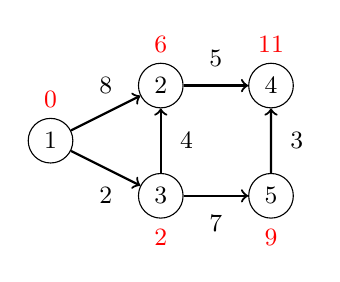
\begin{tikzpicture}[scale=0.7,label distance=0mm]
\small
\node[draw, circle] (1) at (0,-1) {$1$};
\node[draw, circle] (2) at (2,0) {$2$};
\node[draw, circle] (3) at (2,-2) {$3$};
\node[draw, circle] (4) at (4,0) {$4$};
\node[draw, circle] (5) at (4,-2) {$5$};
\path[draw,thick,->] (1) -- node[font=\small,label=above:8] {} (2);
\path[draw,thick,->] (1) -- node[font=\small,label=below:2] {} (3);
\path[draw,thick,->] (3) -- node[font=\small,label=right:4] {} (2);
\path[draw,thick,->] (2) -- node[font=\small,label=above:5] {} (4);
\path[draw,thick,->] (3) -- node[font=\small,label=below:7] {} (5);
\path[draw,thick,->] (5) -- node[font=\small,label=right:3] {} (4);
\node[color=red] at (0,-0.25) {$0$};
\node[color=red] at (2,0.75) {$6$};
\node[color=red] at (2,-2.75) {$2$};
\node[color=red] at (4,0.75) {$11$};
\node[color=red] at (4,-2.75) {$9$};
\end{tikzpicture}
\end{center}
\caption{Lyhimpien polkujen pituudet solmusta $1$ alkaen.}
\label{fig:lypola}
\end{figure}

Tavallisin tilanne käytännön verkko-ongelmissa on,
että haluamme löytää lyhimmän polun solmusta $a$ solmuun $b$.
Yksittäisen lyhimmän polun etsiminen vaatii usein kuitenkin,
että etsimme sitä ennen muitakin lyhimpiä polkuja.
Niinpä keskitymme alusta asti yleisempään ongelmaan,
jossa olemme valinneet jonkin solmun lähtösolmuksi
ja haluamme määrittää \emph{jokaiselle} verkon solmulle,
kuinka pitkä on lyhin polku lähtösol\-musta solmuun
eli mikä on solmun etäisyys lähtösolmusta.

Kuvassa \ref{fig:lypola} on esimerkkinä verkko,
jossa lähtösolmuna on solmu $1$ ja jokaisen solmun
viereen on merkitty sen etäisyys.
Esimerkiksi solmun $5$ etäisyys on $9$,
koska lyhin polku solmusta $1$ solmuun $5$ on
$1 \rightarrow 3 \rightarrow 5$, jonka pituus on $2+7=9$.
Käytämme tätä verkkoa esimerkkinä, kun tutustumme
seuraavaksi kahteen algoritmiin lyhimpien polkujen etsimiseen.

\subsection{Bellmanin ja Fordin algoritmi}

\index{Bellmanin ja Fordin algoritmi}

\emph{Bellmanin ja Fordin algoritmi} etsii lyhimmät polut
annetusta lähtösolmusta kaikkiin verkon solmuihin.
Algoritmi muodostaa taulukon, joka kertoo jokaiselle
verkon solmulle sen etäisyyden lähtösolmusta.
Algoritmi toimii missä tahansa verkossa,
kunhan verkossa ei ole negatiivista sykliä eli sykliä,
jonka painojen summa on negatiivinen.

Bellmanin ja Fordin algoritmi pitää yllä \emph{arvioita}
solmujen etäisyyksistä niin,
että aluksi etäisyys lähtösolmuun on 0 ja etäisyys
kaikkiin muihin solmuihin on ääretön.
Tämän jälkeen algoritmi alkaa parantaa etäisyyksiä
etsimällä verkosta kaaria, joiden kautta kulkeminen
lyhentää polkuja.
Jokaisella askeleella algoritmi etsii kaaren $a \rightarrow b$,
jolle pätee, että pääsemme solmuun $b$ aiempaa lyhempää polkua
kulkemalla kaarella solmusta $a$.
Kun mitään etäisyysarviota ei voi enää parantaa,
algoritmi päättyy ja kaikki etäisyydet vastaavat
todellisia lyhimpien polkujen pituuksia.

\begin{figure}[ht]
\center
\begin{center}
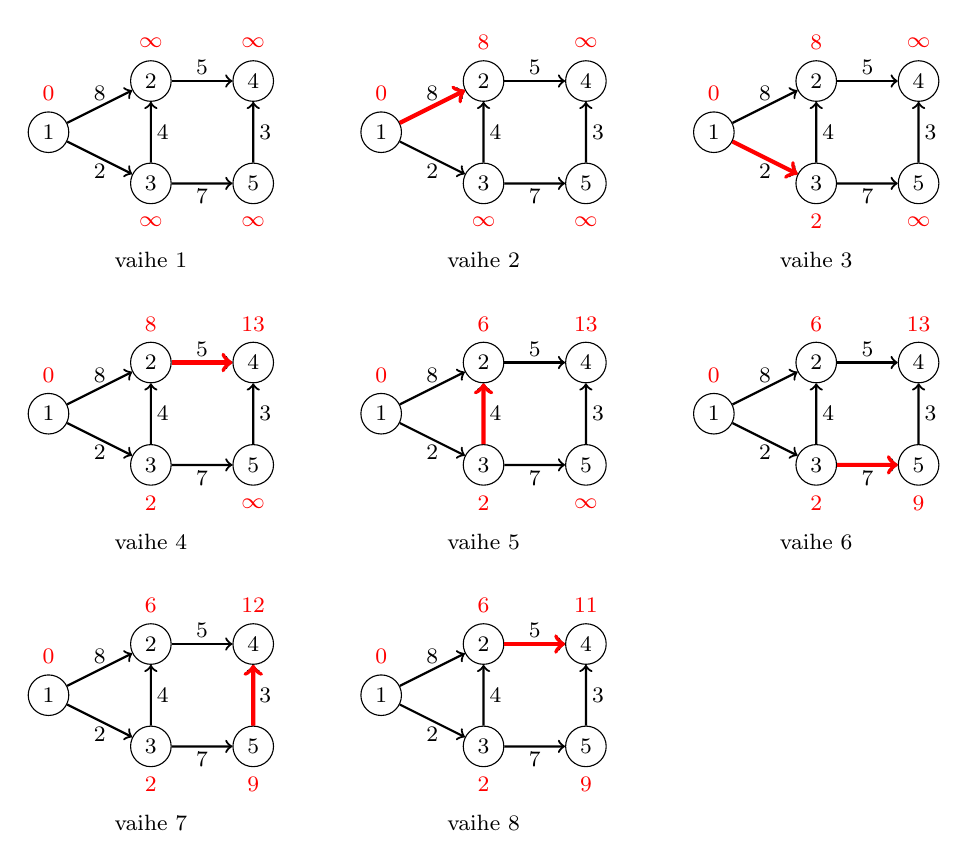
\begin{tikzpicture}[scale=0.65,label distance=-1.5mm]
\footnotesize
\newcommand\verkko[6]{
\node[draw, circle] (1) at (0,-1) {$1$};
\node[draw, circle] (2) at (2,0) {$2$};
\node[draw, circle] (3) at (2,-2) {$3$};
\node[draw, circle] (4) at (4,0) {$4$};
\node[draw, circle] (5) at (4,-2) {$5$};
\path[draw,thick,->] (1) -- node[font=\small,label=above:8] {} (2);
\path[draw,thick,->] (1) -- node[font=\small,label=below:2] {} (3);
\path[draw,thick,->] (3) -- node[font=\small,label=right:4] {} (2);
\path[draw,thick,->] (2) -- node[font=\small,label=above:5] {} (4);
\path[draw,thick,->] (3) -- node[font=\small,label=below:7] {} (5);
\path[draw,thick,->] (5) -- node[font=\small,label=right:3] {} (4);
\node[color=red] at (0,-0.25) {$#2$};
\node[color=red] at (2,0.75) {$#3$};
\node[color=red] at (2,-2.75) {$#4$};
\node[color=red] at (4,0.75) {$#5$};
\node[color=red] at (4,-2.75) {$#6$};
\node at (2,-3.5) {vaihe #1};
}
\begin{scope}
\verkko{1}{0}{\infty}{\infty}{\infty}{\infty}
\end{scope}
\begin{scope}[xshift=6.5cm]
\verkko{2}{0}{8}{\infty}{\infty}{\infty}
\path[draw=red,thick,->,line width=1.5pt] (1) -- (2);
\end{scope}
\begin{scope}[xshift=13cm]
\verkko{3}{0}{8}{2}{\infty}{\infty}
\path[draw=red,thick,->,line width=1.5pt] (1) -- (3);
\end{scope}
\begin{scope}[yshift=-5.5cm]
\verkko{4}{0}{8}{2}{13}{\infty}
\path[draw=red,thick,->,line width=1.5pt] (2) -- (4);
\end{scope}
\begin{scope}[yshift=-5.5cm,xshift=6.5cm]
\verkko{5}{0}{6}{2}{13}{\infty}
\path[draw=red,thick,->,line width=1.5pt] (3) -- (2);
\end{scope}
\begin{scope}[yshift=-5.5cm,xshift=13cm]
\verkko{6}{0}{6}{2}{13}{9}
\path[draw=red,thick,->,line width=1.5pt] (3) -- (5);
\end{scope}
\begin{scope}[yshift=-11cm]
\verkko{7}{0}{6}{2}{12}{9}
\path[draw=red,thick,->,line width=1.5pt] (5) -- (4);
\end{scope}
\begin{scope}[yshift=-11cm,xshift=6.5cm]
\verkko{8}{0}{6}{2}{11}{9}
\path[draw=red,thick,->,line width=1.5pt] (2) -- (4);
\end{scope}
\end{tikzpicture}
\end{center}
\caption{Esimerkki Bellmanin ja Fordin algoritmin toiminnasta.}
\label{fig:belfor}
\end{figure}

Kuva \ref{fig:belfor} näyttää esimerkin Bellmanin ja Fordin algoritmin toiminnasta,
kun lähtösolmuna on solmu $1$.
Jokaisen solmun vieressä on ilmoitettu sen etäisyysarvio:
aluksi etäisyys solmuun 1 on 0 ja etäisyys kaikkiin muihin solmuihin on ääretön.
Jokainen etäisyyden muutos näkyy kuvassa omana vaiheenaan.
Ensin parannamme etäisyyttä solmuun 2
kulkemalla kaarta $1 \rightarrow 2$,
jolloin etäisyydeksi tulee $8$.
Sitten parannamme etäisyyttä solmuun $3$
kulkemalla kaarta $1 \rightarrow 3$,
jolloin solmun uudeksi etäisyydeksi tulee $2$.
Jatkamme samalla tavalla, kunnes emme voi enää parantaa
mitään etäisyyttä ja kaikki etäisyydet
vastaavat lyhimpien polkujen pituuksia.

Bellmanin ja Fordin algoritmi on mukavaa toteuttaa
käyttäen verkon kaarilistaesitystä,
jossa jokaisesta kaaresta on tallennettu alku- ja loppusolmu sekä paino.
Toteutamme algoritmin niin,
että se muodostuu \emph{kierroksista},
joista jokainen käy läpi kaikki verkon kaaret
ja koettaa parantaa etäisyysarvioita niiden avulla.
Voimme toteuttaa algoritmin näin:

\begin{code}
while true
    muutos = false
    for kaari in kaaret
        nyky = etaisyys[kaari.loppu]
        uusi = etaisyys[kaari.alku]+kaari.paino
        if uusi < nyky
            etaisyys[kaari.loppu] = uusi
            muutos = true
    if not muutos
        break
\end{code}

Algoritmi käy jokaisella kierroksella läpi verkon kaaret
ja tutkii kunkin kaaren kohdalla,
mikä on nykyinen etäisyys kaaren kohdesolmuun
sekä mikä on uusi etäisyys, jos kuljemmekin solmuun kaaren kautta.
Jos uusi etäisyys on pienempi, päivitämme
sen solmun etäisyysarvioksi.
Muuttujassa \texttt{muutos} on tieto siitä,
onko jokin etäisyys muuttunut kierroksen aikana,
ja algoritmi päättyy, kun mikään etäisyys ei muuttunut.

\subsubsection{Algoritmin analyysi}

Olemme nyt kuvailleet ja toteuttaneet Bellmanin ja Fordin
algoritmin, mutta miten voimme olla varmoja,
että se löytää lyhimmät polut, ja miten nopeasti se toimii?
Jotta voimme vastata näihin kysymyksiin,
tarvitsemme kaksi havaintoa koskien verkon lyhimpiä polkuja.

Ensimmäinen havainto on, että jos
$s_1 \rightarrow s_2 \rightarrow \dots \rightarrow s_k$ on
lyhin polku solmusta $s_1$ solmuun $s_k$,
niin myös $s_1 \rightarrow s_2$ on lyhin polku solmusta $s_1$ solmuun $s_2$,
$s_1 \rightarrow s_2 \rightarrow s_3$ on lyhin polku solmusta $s_1$ solmuun $s_3$, jne.,
eli jokainen lyhimmän polun alkuosa on myös lyhin polku vastaavaan solmuun.
Jos näin ei olisi, voisimme parantaa lyhintä polkua solmusta $s_1$ solmuun $s_k$
parantamalla jotain polun alkuosaa, mikä aiheuttaisi ristiriidan.

Toinen havainto on,
että $n$ solmun verkossa jokainen lyhin polku voi
sisältää enintään $n-1$ kaarta,
kun oletamme, että verkossa ei ole negatiivista sykliä.
Jos polkuun kuuluisi $n$ kaarta tai enemmän,
jokin solmu esiintyisi polulla monta kertaa.
Tämä ei ole kuitenkaan mahdollista,
koska ei olisi järkeä kulkea monta kertaa saman solmun kautta,
kun haluamme saada aikaan lyhimmän polun.

Tarkastellaan nyt, mitä tapahtuu algoritmin kierroksissa.
Ensimmäisen kierroksen jälkeen olemme löytäneet lyhimmät polut,
joissa on enintään yksi kaari.
Toisen kierroksen jälkeen olemme löytäneet lyhimmät polut,
joissa on enintään kaksi kaarta.
Sama jatkuu, kunnes $n-1$ kierroksen jälkeen olemme löytäneet
lyhimmät polut, joissa on enintään $n-1$ kaarta.
Koska missään lyhimmässä polussa ei voi olla enempää kaaria,
olemme löytäneet kaikki lyhimmät polut.
Algoritmin riittää suorittaa siis enintään $n-1$ kierrosta,
joista jokainen käy läpi kaikki verkon kaaret ajassa $O(m)$.
Niinpä algoritmi löytää kaikki lyhimmät polut ajassa $O(nm)$.

\begin{figure}
\center
\begin{center}
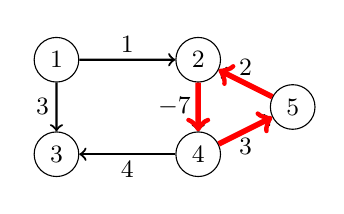
\begin{tikzpicture}[scale=0.6,label distance=-1.5mm]
\small
\node[draw, circle] (1) at (1,3) {$1$};
\node[draw, circle] (2) at (4,3) {$2$};
\node[draw, circle] (3) at (1,1) {$3$};
\node[draw, circle] (4) at (4,1) {$4$};
\node[draw, circle] (5) at (6,2) {$5$};

\path[draw,thick,->] (1) -- node[font=\small,label=above:1] {} (2);
\path[draw,thick,->] (1) -- node[font=\small,label=left:3] {} (3);
\path[draw,thick,<-] (3) -- node[font=\small,label=below:4] {} (4);
\path[draw,thick,->] (2) -- node[font=\small,label=left:$-7$] {} (4);
\path[draw,thick,<-] (2) -- node[font=\small,label=above:2] {} (5);
\path[draw,thick,->] (4) -- node[font=\small,label=below:3] {} (5);

\path[draw,thick,->,red,line width=2pt] (2) -- (4);
\path[draw,thick,->,red,line width=2pt] (4) -- (5);
\path[draw,thick,->,red,line width=2pt] (5) -- (2);

\end{tikzpicture}
\end{center}
\caption{Negatiivinen sykli $2 \rightarrow 4 \rightarrow 5 \rightarrow 2$,
jonka avulla voimme lyhentää polkuja loputtomasti.}
\label{fig:belsyk}
\end{figure}

Mitä tapahtuu sitten, jos verkossa on negatiivinen sykli?
Esimerkiksi kuvan \ref{fig:belsyk} verkossa on negatiivinen sykli
$2 \rightarrow 4 \rightarrow 5 \rightarrow 2$, jonka paino on $-2$.
Tässä tilanteessa Bellmanin ja Fordin algoritmi jatkuu ikuisesti,
koska voimme lyhentää loputtomasti syklin kautta kulkevia polkuja.
Oikeastaan ongelma on siinä, että lyhin polku ei ole mielekäs käsite,
jos polun osana on negatiivinen sykli.
Voimme kuitenkin havaita verkossa olevan negatiivisen syklin
Bellmanin ja Fordin algoritmin avulla:
jos jotain etäisyyttä voi parantaa vielä $n-1$ kierroksen jälkeen,
verkossa on negatiivinen sykli.

\subsection{Dijkstran algoritmi}

\index{Dijkstran algoritmi}

\emph{Dijkstran algoritmi} on Bellmanin ja Fordin algoritmin tehostettu versio,
jonka toiminta perustuu oletukseen, että verkossa ei ole
negatiivisen painoisia kaaria.
Bellmanin ja Fordin algoritmin tapaan Dijkstran algoritmi pitää
yllä arvioita etäisyyksistä lähtösolmusta muihin solmuihin.
Erona on kuitenkin tapa, miten Dijkstran algoritmi parantaa etäisyyksiä.

Dijkstran algoritmissa verkon solmut kuuluvat kahteen luokkaan:
käsitte\-lemättömiin ja käsiteltyihin.
Aluksi kaikki solmut ovat käsittelemättömiä.
Algoritmi etsii joka askeleella käsittelemättömän solmun,
jonka etäisyys\-arvio on pienin.
Sitten algoritmi käy läpi kaikki solmusta lähtevät kaaret ja
koettaa parantaa etäisyyksiä niiden avulla.
Tämän jälkeen solmu on käsitelty eikä sen etäisyys enää muutu,
eli aina kun olemme käsitelleet solmun,
olemme saaneet selville sen lopullisen etäisyyden.

\begin{figure}
\center
\begin{center}
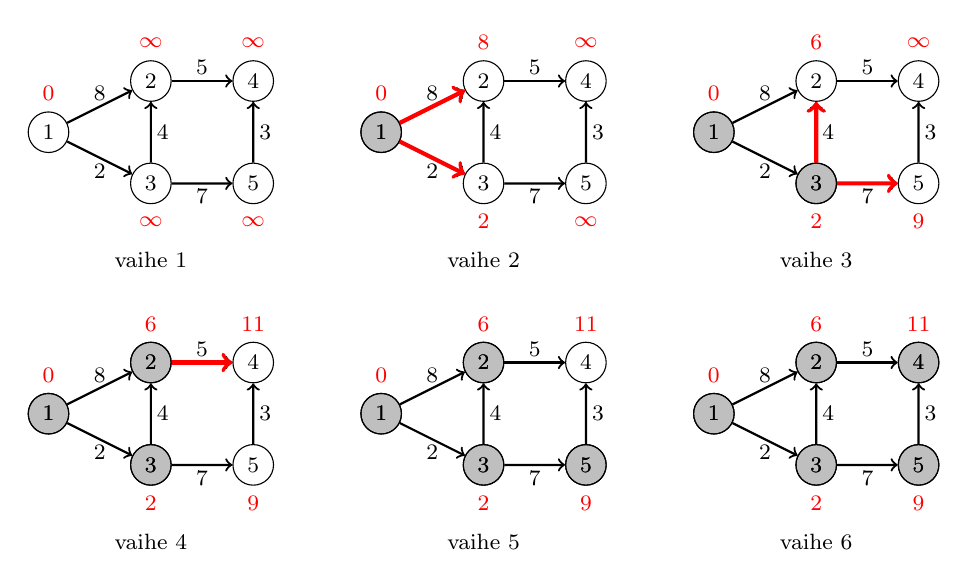
\begin{tikzpicture}[scale=0.65,label distance=-1.5mm]
\footnotesize
\newcommand\verkko[6]{
\node[draw, circle] (1) at (0,-1) {$1$};
\node[draw, circle] (2) at (2,0) {$2$};
\node[draw, circle] (3) at (2,-2) {$3$};
\node[draw, circle] (4) at (4,0) {$4$};
\node[draw, circle] (5) at (4,-2) {$5$};
\path[draw,thick,->] (1) -- node[font=\small,label=above:8] {} (2);
\path[draw,thick,->] (1) -- node[font=\small,label=below:2] {} (3);
\path[draw,thick,->] (3) -- node[font=\small,label=right:4] {} (2);
\path[draw,thick,->] (2) -- node[font=\small,label=above:5] {} (4);
\path[draw,thick,->] (3) -- node[font=\small,label=below:7] {} (5);
\path[draw,thick,->] (5) -- node[font=\small,label=right:3] {} (4);
\node[color=red] at (0,-0.25) {$#2$};
\node[color=red] at (2,0.75) {$#3$};
\node[color=red] at (2,-2.75) {$#4$};
\node[color=red] at (4,0.75) {$#5$};
\node[color=red] at (4,-2.75) {$#6$};
\node at (2,-3.5) {vaihe #1};
}
\begin{scope}
\verkko{1}{0}{\infty}{\infty}{\infty}{\infty}
\end{scope}
\begin{scope}[xshift=6.5cm]
\node[draw, circle, fill=lightgray] (1) at (0,-1) {$1$};
\verkko{2}{0}{8}{2}{\infty}{\infty}
\path[draw=red,thick,->,line width=1.5pt] (1) -- (2);
\path[draw=red,thick,->,line width=1.5pt] (1) -- (3);
\end{scope}
\begin{scope}[xshift=13cm]
\node[draw, circle, fill=lightgray] (1) at (0,-1) {$1$};
\node[draw, circle, fill=lightgray] (3) at (2,-2) {$3$};
\verkko{3}{0}{6}{2}{\infty}{9}
\path[draw=red,thick,->,line width=1.5pt] (3) -- (2);
\path[draw=red,thick,->,line width=1.5pt] (3) -- (5);
\end{scope}
\begin{scope}[yshift=-5.5cm]
\node[draw, circle, fill=lightgray] (1) at (0,-1) {$1$};
\node[draw, circle, fill=lightgray] (3) at (2,-2) {$3$};
\node[draw, circle, fill=lightgray] (2) at (2,0) {$2$};
\verkko{4}{0}{6}{2}{11}{9}
\path[draw=red,thick,->,line width=1.5pt] (2) -- (4);
\end{scope}
\begin{scope}[yshift=-5.5cm,xshift=6.5cm]
\node[draw, circle, fill=lightgray] (1) at (0,-1) {$1$};
\node[draw, circle, fill=lightgray] (3) at (2,-2) {$3$};
\node[draw, circle, fill=lightgray] (2) at (2,0) {$2$};
\node[draw, circle, fill=lightgray] (5) at (4,-2) {$5$};
\verkko{5}{0}{6}{2}{11}{9}
\end{scope}
\begin{scope}[yshift=-5.5cm,xshift=13cm]
\node[draw, circle, fill=lightgray] (1) at (0,-1) {$1$};
\node[draw, circle, fill=lightgray] (3) at (2,-2) {$3$};
\node[draw, circle, fill=lightgray] (2) at (2,0) {$2$};
\node[draw, circle, fill=lightgray] (5) at (4,-2) {$5$};
\node[draw, circle, fill=lightgray] (4) at (4,0) {$4$};
\verkko{6}{0}{6}{2}{11}{9}
\end{scope}
\end{tikzpicture}
\end{center}
\caption{Esimerkki Dijkstran algoritmin toiminnasta.}
\label{fig:dijalg}
\end{figure}

Kuva \ref{fig:dijalg} näyttää esimerkin Dijkstran algoritmin
toiminnasta.
Solmun harmaa väri tarkoittaa, että se on käsitelty.
Aluksi valitsemme käsittelyyn solmun 1, koska sen etäisyys 0 on pienin.
Sitten jäljellä ovat solmut 2, 3, 4 ja 5,
joista valitsemme käsittelyyn solmun 3, jonka etäisyys 2 on pienin.
Tämän jälkeen valitsemme käsittelyyn solmun 2,
jonka etäisyys on 6.
Sama jatkuu, kunnes olemme käsitelleet kaikki verkon solmut.

Dijkstran algoritmissa etsimme $n$ kertaa
käsittelemättömän solmun, jonka etäisyysarvio on pienin.
Koska haluamme saada algoritmista tehokkaan,
meidän täytyy pystyä löytämään solmut nopeasti.
Tavallinen tapa toteuttaa Dijkstran algoritmi on käyttää \emph{kekoa},
jonka avulla löydämme joka vaiheessa pienimmän etäisyyden solmun
logaritmisessa ajassa.
Tallennamme kekoon pareja, joissa on solmun etäisyys ja tunnus
ja jotka järjestetään etäisyyden mukaan pienimmästä suurimpaan.
Aluksi keossa on vain lähtösolmua vastaava solmu,
jonka etäisyys on $0$.
Tämän jälkeen haemme joka askeleella keosta solmun,
jonka etäisyys on pienin.
Jos solmu on jo käsitelty, emme tee mitään.
Muuten käymme läpi kaikki solmusta lähtevät kaaret
ja tarkastamme, voimmeko parantaa etäisyyksiä
niiden avulla.
Aina kun voimme parantaa etäisyyttä,
lisäämme uuden etäisyyden kekoon.

Dijkstran algoritmi on mukavaa toteuttaa käyttäen
verkon vieruslistaesitystä.
Voimme toteuttaa algoritmin seuraavasti:

\begin{code}
keko.push((0,alku))
while not keko.empty()
    solmu = keko.pop()[1]
    if kasitelty[solmu]
        continue
    kasitelty[solmu] = true
    for kaari in verkko[solmu]
        nyky = etaisyys[kaari.loppu]
        uusi = etaisyys[solmu]+kaari.paino
        if uusi < nyky
            etaisyys[kaari.loppu] = uusi
            keko.push((uusi,kaari.loppu))
\end{code}

Huomaa, että keossa voi olla samaan aikaan \emph{useita} etäisyyksiä
samalle solmulle, koska lisäämme kekoon uuden solmun
aina etäisyyden parantuessa.
Käsittelemme kuitenkin jokaisen solmun vain kerran,
koska aina kun olemme hakeneet uuden solmun keosta käsittelyä varten,
varmistamme ensin, että emme ole käsitelleet sitä aiemmin.

\subsubsection{Algoritmin analyysi}

Dijkstran algoritmi on ahne algoritmi,
koska se etsii joka vaiheessa
vielä käsittelemättömän solmun,
jonka etäisyys on pienin, minkä jälkeen kyseisen
solmun etäisyys ei enää muutu.
Miten voimme olla varmoja, että olemme löytäneet
tässä vaiheessa oikean etäisyyden?

Voimme ajatella asiaa siltä kannalta,
että jos etäisyyttä olisi mahdollista parantaa,
niin verkossa olisi oltava jokin toinen vielä
käsittelemätön solmu, jonka kautta voisimme muodostaa lyhemmän polun.
Kuitenkin tiedämme, että kaikkien muiden tarjolla olevien solmujen
etäisyydet ovat suurempia tai yhtä suuria eivätkä etäisyydet voi lyhentyä,
koska verkossa ei ole negatiivisia kaaria.
Tästä syystä voimme turvallisesti valita käsittelyyn pienimmän etäisyyden
solmun ja kiinnittää sen etäisyyden.

\begin{figure}
\center
\begin{center}
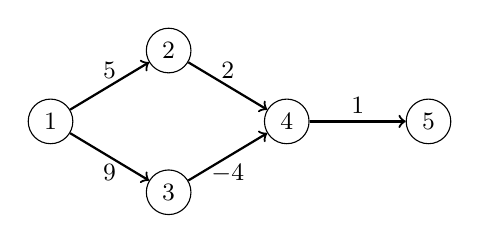
\begin{tikzpicture}[scale=0.6,label distance=-1.5mm]
\small
\node[draw, circle] (1) at (0,1) {$1$};
\node[draw, circle] (2) at (2.5,2.5) {$2$};
\node[draw, circle] (3) at (2.5,-0.5) {$3$};
\node[draw, circle] (4) at (5,1) {$4$};
\node[draw, circle] (5) at (8,1) {$5$};

\path[draw,thick,->] (1) -- node[font=\small,label=above:5] {} (2);
\path[draw,thick,->] (1) -- node[font=\small,label=below:9] {} (3);
\path[draw,thick,->] (2) -- node[font=\small,label=above:2] {} (4);
\path[draw,thick,->] (3) -- node[font=\small,label=below:$-4$] {} (4);
\path[draw,thick,->] (4) -- node[font=\small,label=above:1] {} (5);
\end{tikzpicture}
\end{center}
\caption{Dijkstran algoritmi ei toimi oikein negatiivisen kaaren takia.}
\label{fig:dijneg}
\end{figure}

Dijkstran algoritmi toimii siis oikein,
jos verkossa ei ole negatiivisia kaaria,
mutta kuinka nopeasti algoritmi toimii?
Ensinnäkin algoritmi käy läpi verkon solmut
ja kaaret, missä kuluu aikaa $O(n+m)$.
Lisäksi algoritmissa on joukko kekoon liittyviä operaatioita,
jotka vaikuttavat tehokkuuteen.
Pahimmassa tapauksessa lisäämme jokaisen kaaren kohdalla
kekoon uuden alkion, eli lisäykset kekoon vievät aikaa $O(m \log m)$.
Toisaalta poistamme kaikki alkiot aikanaan keosta,
mihin menee myös aikaa $O(m \log m)$.
Algoritmin kokonaisaikavaativuus on siis $O(n + m \log m)$.

Voimme vielä hieman siistiä aikavaativuutta, kun
teemme luontevan oletuksen,
että verkossa ei ole kahta kaarta, joiden alku- ja loppusolmu ovat samat.
Tällöin $m \le n^2$, jolloin $\log m = \log (n^2) = 2 \log n$
ja saamme algoritmin aikavaativuudeksi $O(n+m \log n)$.

Entä mitä tapahtuu, jos verkossa kuitenkin on negatiivinen kaari?
Tällöin Dijkstran algoritmi ei toimi välttämättä oikein.
Kuva \ref{fig:dijneg} näyttää esimerkin tällaisesta tilanteesta.
Algoritmi seuraa ahneesti ylempää polkua ja toteaa,
että pienin etäisyys solmusta 1 solmuun 5 on 8.
Kuitenkin parempi tapa olisi kulkea alempaa polkua,
jolloin polun pituus on vain 6.

\subsection{Esimerkki: Reittiopas}

Nyt meillä on tarvittavat tiedot,
joiden avulla voimme luoda \emph{reittioppaan}
eli järjestelmän, jonka avulla voi etsiä
eri kulkuvälineitä käyttäviä reittejä kaupungissa.
Voimme mallintaa kaupungin verkkona,
jonka solmut ovat kaupungin paikkoja ja kaaret
ovat mahdollisia yhteyksiä paikkojen välillä.
Reittioppaan tulisi ilmoittaa \emph{nopein} reitti
paikasta $a$ paikkaan $b$.

Reittioppaan toteuttamiseen liittyy yksi lisähaaste:
kulkuvälineillä on tietyt aikataulut,
jotka rajoittavat niiden käyttöä.
Esimerkiksi bussilinjan lähtöjä saattaa olla
10 minuutin välein.
Meidän tulee siis ottaa huomioon reitin etsimisessä,
mihin aikaan saavumme mihinkin paikkaan.
Voimme toteuttaa tämän tallentamalla verkon kaaret
muodossa ''matka alkaa ajanhetkenä $x$ ja
päättyy ajanhetkenä $y$''.

Koska kaikissa matkoissa kuluu positiivinen määrä aikaa,
voimme etsiä reittejä Dijkstran algoritmin avulla.
Toteutamme algoritmin niin,
että määritämme jokaiseen paikkaan \emph{varhaisimman}
ajan, jolloin voimme päästä kyseiseen paikkaan.
Alussa tiedämme, että olemme lähtöpaikassa
matkamme alkuhetkenä.
Sitten kun otamme käsittelyyn uuden paikan,
käymme läpi siitä lähteviä yhteyksiä,
joihin ehdimme optimaalista aikataulua noudattaen.
Saamme tehostettua hakua merkittävästi ottamalla
huomioon jokaisesta linjasta vain ensimmäisen lähdön,
johon ehdimme.
Tämä on perusteltua, koska ei voi missään tilanteessa
olla hyvä idea odottaa myöhempään lähtöön.

\begin{figure}
\center
\begin{center}
\begin{tikzpicture}[scale=0.6,label distance=-1.5mm]
\begin{scope}
\small
\node[draw, circle] (1) at (0,0) {$1$};
\node[draw, circle] (2) at (3,1) {$2$};
\node[draw, circle] (3) at (4,-1) {$3$};
\node at (0,-1) {13:15};
\node at (3,2) {?};
\node at (4,-2) {?};
\path[draw,thick,->] (1) -- (2);
\path[draw,thick,->] (1) -- (3);
\path[draw,thick,->] (2) -- (3);
\node at (2,-3) {(a)};
\end{scope}
\begin{scope}[xshift=8cm]
\small
\node[draw, circle, fill=lightgray] (1) at (0,0) {$1$};
\node[draw, circle] (2) at (3,1) {$2$};
\node[draw, circle] (3) at (4,-1) {$3$};
\node at (0,-1) {13:15};
\node at (3,2) {13:27};
\node at (4,-2) {13:40};
\path[draw,thick,->] (1) -- (2);
\path[draw,thick,->] (1) -- (3);
\path[draw,thick,->] (2) -- (3);
\node at (2,-3) {(b)};
\end{scope}
\begin{scope}[xshift=16cm]
\small
\node[draw, circle, fill=lightgray] (1) at (0,0) {$1$};
\node[draw, circle, fill=lightgray] (2) at (3,1) {$2$};
\node[draw, circle] (3) at (4,-1) {$3$};
\node at (0,-1) {13:15};
\node at (3,2) {13:27};
\node at (4,-2) {13:32};
\path[draw,thick,->] (1) -- (2);
\path[draw,thick,->] (1) -- (3);
\path[draw,thick,->] (2) -- (3);
\node at (2,-3) {(c)};
\end{scope}
\end{tikzpicture}
\end{center}
\caption{Nopeimman reitin etsiminen paikasta $1$ paikkaan $3$.
(a) Matka alkaa kello 13:15. (b) Käymme läpi paikasta 2 lähtevät yhteydet.
(c) Käymme läpi paikasta 3 lähtevät yhteydet.}
\label{fig:reiopa}
\end{figure}

Kuva \ref{fig:reiopa} näyttää esimerkkitilanteen,
jossa haluamme kulkea paikasta $1$ paikkaan $3$ ja
lähdemme matkaan kello 13:15.
Paikasta $1$ lähtee 10 minuutin välein
yhteys paikkaan $2$ (kesto 7 minuuttia)
sekä 30 minuutin välein yhteys paikkaan $3$ (kesto 10 minuuttia).
Niinpä pääsemme paikkaan $2$ kello 13:27 ja paikkaan 3 kello 13:40.
Sitten paikasta $2$ lähtee 5 minuutin välein yhteys paikkaan $3$
(kesto 2 minuuttia).
Tämän avulla pääsemme paikkaan $3$ kello 13:32,
eli nopein reitti kulkee paikan $2$ kautta.

Käytännössä hakua voisi vielä tehostaa monella tavalla.
Esimerkiksi kun löydämme jonkin reitin kohdepaikkaan,
voimme siitä lähtien hylätä kaikki paikat,
joihin ehdimme myöhemmin kuin kohdepaikkaan.

\section{Kaikki lyhimmät polut}

Tarkastellaan seuraavaksi ongelmaa, jossa
haluamme etsiä lyhimmät polut verkon
\emph{kaikista} solmuista \emph{kaikkiin} solmuihin.
Yksi tapa ratkaista tehtävä olisi suorittaa Bellmanin ja Fordin
tai Dijkstran algoritmi jokaisesta verkon solmusta alkaen.
Voimme kuitenkin ratkaista tehtävän suoremmin
etsimällä kaikki polut \emph{samanaikaisesti}
Floydin ja Warshallin algoritmilla.

\subsection{Floydin ja Warshallin algoritmi}

\index{Floydin ja Warshallin algoritmi}
\index{etäisyysmatriisi}

\emph{Floydin ja Warshallin algoritmi} muodostaa $n \times n$ -kokoisen
\emph{etäisyysmatriisin} (\emph{distance matrix}),
jossa rivin $a$ sarakkeessa $b$ on lyhimmän polun pituus
solmusta $a$ solmuun $b$.
Algoritmi alustaa ensin matriisin niin,
että siihen on merkitty vain etäisyydet,
jotka toteutuvat kulkemalla yksittäistä kaarta,
ja kaikissa muissa matriisin kohdissa etäisyys on ääretön.
Sitten algoritmi suorittaa $n$ kierrosta,
jotka on numeroitu $1,2,\dots,n$.
Kierroksella $k$ algoritmi etsii polkuja, joissa on välisolmuna
solmu $k$ sekä mahdollisesti muita välisolmuja joukosta $1,2,\dots,k-1$.
Jos tällainen polku parantaa etäisyyttä,
päivitämme uuden etäisyyden matriisiin.
Lopulta jokainen solmu on ollut
välisolmuna poluilla, jolloin olemme saaneet selville
kaikki lyhimmät polut.

\begin{figure}
\center
\begin{center}
\begin{tikzpicture}[scale=0.6,label distance=-1.5mm]
\small
\newcommand\verkko[5]{
\begin{scope}[xshift=0.75cm,yshift=2cm]
\node[draw, circle, fill=#2] (1) at (0,0) {$1$};
\node[draw, circle, fill=#3] (2) at (2.5,0) {$2$};
\node[draw, circle, fill=#4] (3) at (0,-2.5) {$3$};
\node[draw, circle, fill=#5] (4) at (2.5,-2.5) {$4$};
\path[draw,thick,->] (1) -- node[font=\small,label=above:5] {} (2);
\path[draw,thick,->] (1) -- node[font=\small,label=left:1] {} (3);
\path[draw,thick,->] (2) -- node[font=\small,label=right:3] {} (4);
\path[draw,thick,->] (3) -- node[font=\small,label=above:2] {} (2);
\path[draw,thick,->] (4) -- node[font=\small,label=below:4] {} (3);
\end{scope}

\foreach \x in {1,2,3,4} \node at (-0.5,-2.5-\x) {\x};
\foreach \x in {1,2,3,4} \node at (-0.5+\x,-2.5) {\x};
\draw (0,-3) grid (4,-7);

\node at (2,-8) {kierros #1};
}
\begin{scope}
\verkko{1}{lightgray}{white}{white}{white}
\foreach \x/\v in {1/0,2/5,3/1,4/\infty} \node at (-0.5+\x,-3.5) {$\v$};
\foreach \x/\v in {1/\infty,2/0,3/\infty,4/3} \node at (-0.5+\x,-4.5) {$\v$};
\foreach \x/\v in {1/\infty,2/2,3/0,4/\infty} \node at (-0.5+\x,-5.5) {$\v$};
\foreach \x/\v in {1/\infty,2/\infty,3/4,4/0} \node at (-0.5+\x,-6.5) {$\v$};
\end{scope}
\begin{scope}[xshift=5.5cm]
\verkko{2}{white}{lightgray}{white}{white}
\foreach \x/\v in {1/0,2/5,3/1,4/} \node at (-0.5+\x,-3.5) {$\v$};
\foreach \x/\v in {1/\infty,2/0,3/\infty,4/3} \node at (-0.5+\x,-4.5) {$\v$};
\foreach \x/\v in {1/\infty,2/2,3/0,4/} \node at (-0.5+\x,-5.5) {$\v$};
\foreach \x/\v in {1/\infty,2/\infty,3/4,4/0} \node at (-0.5+\x,-6.5) {$\v$};
\node[color=red] at (3.5,-3.5) {$8$};
\node[color=red] at (3.5,-5.5) {$5$};
\end{scope}
\begin{scope}[xshift=11cm]
\verkko{3}{white}{white}{lightgray}{white}
\foreach \x/\v in {1/0,2/,3/1,4/} \node at (-0.5+\x,-3.5) {$\v$};
\foreach \x/\v in {1/\infty,2/0,3/\infty,4/3} \node at (-0.5+\x,-4.5) {$\v$};
\foreach \x/\v in {1/\infty,2/2,3/0,4/5} \node at (-0.5+\x,-5.5) {$\v$};
\foreach \x/\v in {1/\infty,2/,3/4,4/0} \node at (-0.5+\x,-6.5) {$\v$};
\node[color=red] at (1.5,-3.5) {$3$};
\node[color=red] at (1.5,-6.5) {$6$};
\node[color=red] at (3.5,-3.5) {$6$};
\end{scope}
\begin{scope}[xshift=16.5cm]
\verkko{4}{white}{white}{white}{lightgray}
\foreach \x/\v in {1/0,2/3,3/1,4/6} \node at (-0.5+\x,-3.5) {$\v$};
\foreach \x/\v in {1/\infty,2/0,3/,4/3} \node at (-0.5+\x,-4.5) {$\v$};
\foreach \x/\v in {1/\infty,2/2,3/0,4/5} \node at (-0.5+\x,-5.5) {$\v$};
\foreach \x/\v in {1/\infty,2/6,3/4,4/0} \node at (-0.5+\x,-6.5) {$\v$};
\node[color=red] at (2.5,-4.5) {$7$};
\end{scope}
\end{tikzpicture}
\end{center}
\caption{Esimerkki Floydin ja Warshallin algoritmin toiminnasta.}
\label{fig:flowar}
\end{figure}

Kuva \ref{fig:flowar} näyttää esimerkin Floydin ja Warshallin algoritmin toiminnasta.
Kierroksella 1 etsimme polkuja, joissa solmu 1 on välisolmuna.
Tällaisia polkuja ei ole, koska solmuun 1 ei pääse mistään solmusta,
joten matriisi ei muutu.
Kierroksella 2 huomaamme, että voimme kulkea solmun 2 kautta
solmusta 1 solmuun 4, jolloin saamme etäisyyden 8.
Samoin voimme kulkea solmun 2 kautta solmusta 3 solmuun 4,
jolloin saamme etäisyyden 5.
Jatkamme vastaavasti, kunnes kierroksen 4 jälkeen olemme
saaneet selville kaikki etäisyydet ja etäisyysmatriisi on lopullinen.

Floydin ja Warshallin algoritmin mukavana puolena on,
että se on hyvin helppoa toteuttaa.
Meidän riittää luoda kolme sisäkkäistä for-silmukkaa,
jotka toteuttavat matriisin päivitykset.
Seuraavassa koodissa muuttuja $k$ kertoo,
mikä kierros on kyseessä eli mitä solmua käytämme välisolmuna.
Jokaisella kierroksella käymme läpi kaikki solmuparit $(i,j)$
ja koetamme parantaa niiden etäisyyksiä kulkemalla solmun $k$ kautta.

\begin{code}
for k = 1 to n
    for i = 1 to n
        for j = 1 to n
            etaisyys[i][j] = min(etaisyys[i][j],
                                   etaisyys[i][k]+etaisyys[k][j])
\end{code}

Algoritmin aikavaativuus on selkeästi $O(n^3)$,
koska se muodostuu kolmesta sisäkkäisestä for-silmukasta.

\subsubsection{Algoritmin analyysi}

Miksi Floydin ja Warshallin algoritmi toimii?
Voimme ymmärtää algoritmia tarkastelemalla
sen toimintaa ''käänteisesti'' rekursiivisesti.
Kun verkossa on lyhin polku solmusta $a$ solmuun $b$,
millainen tämä polku voi olla?

Yksi mahdollisuus on, että polku on vain kaari
solmusta $a$ solmuun $b$.
Tällöin sen pituus on merkitty etäisyysmatriisiin
algoritmin alussa.
Muussa tapauksessa polussa on yksi tai useampi välisolmu.
Oletetaan, että $x$ on välisolmu, jonka tunnus on suurin.
Saamme nyt kaksi osatehtävää:
meidän tulee ensin kulkea solmusta $a$ solmuun $x$
ja sen jälkeen solmusta $x$ solmuun $b$ niin,
että kummallakin polulla jokaisen välisolmun
tunnus on pienempi kuin $x$.
Voimme käsitellä nämä osatehtävät rekursiivisesti.

Floydin ja Warshallin algoritmi muodostaa joka vaiheessa
polkuja, joissa voi olla välisolmuina solmuja $1,2,\dots,i$.
Kun haluamme muodostaa lyhimmän polun solmusta $a$ solmuun $b$,
meillä on kaksi vaihtoehtoa:
Jos solmu $i$ on välisolmuna, yhdistämme lyhimmän polun
solmusta $a$ solmuun $i$ ja solmusta $i$ solmuun $b$.
Jos taas solmu $i$ ei ole välisolmuna, olemme käsitelleet
polun jo aiemmin.
Algoritmin päätteeksi välisolmuina voi olla solmuja $1,2,\dots,n$,
eli mikä tahansa verkon solmu voi olla välisolmu.

\subsection{Algoritmien vertailua}

Olemme nyt käyneet läpi monia algoritmeja
lyhimpien polkujen etsintään ja voimme alkaa
muodostaa yleiskuvaa aiheesta.
Taulukko \ref{tab:reiver} näyttää yhteenvedon
algoritmiemme tehokkuudesta ja ominaisuuksista.

Käytännössä leveyshaku ja Dijkstran algoritmi ovat
yleisimmin tarvittavat algoritmit:
jos kaarilla ei ole painoja, käytämme leveyshakua,
ja muuten Dijkstran algoritmia.
Dijkstran algoritmin rajoituksena on,
että verkossa ei saa olla negatiivisia kaaria,
mutta tällä rajoituksella ei ole yleensä merkitystä
käytännön ongelmissa, koska kaarten painot eivät
useimmiten voi olla negatiivisia.
Esimerkiksi selvästikään tien pituus tai lennon hinta
ei voi olla negatiivinen.
Jos kuitenkin verkossa voi olla negatiivisia kaaria,
voimme turvautua Bellmanin ja Fordin algoritmiin.

\begin{table}
\center
\begin{tabular}{lll}
algoritmi & aikavaativuus & erityistä \\
\hline
leveyshaku & $O(n+m)$ & ei salli painoja kaarissa \\
Bellmanin ja Fordin algoritmi & $O(nm)$ & \\
Dijkstran algoritmi & $O(n+m \log n)$ & ei salli negatiivisia kaaria \\
Floydin ja Warshallin algoritmi & $O(n^3)$ & etsii kaikki polut \\
\end{tabular}
\caption{Algoritmit lyhimpien polkujen etsimiseen.}
\label{tab:reiver}
\end{table}

\index{harva verkko}
\index{tiheä verkko}

Miten sitten Floydin ja Warshallin algoritmi vertautuu muihin algoritmeihin?
Tämä riippuu siitä, onko verkko \emph{harva} (\emph{sparse}) vai
\emph{tiheä} (\emph{dense}).
Harvassa verkossa on vähän kaaria ja $m \approx n$,
kun taas tiheässä verkossa on paljon kaaria ja $m \approx n^2$.
Floydin ja Warshallin algoritmi on parhaimmillaan silloin,
kun verkko on tiheä, koska sen aikavaativuus ei riipu
kaarten määrästä.
Esimerkiksi jos etsimme kaikki lyhimmät polut
suorittamalla $n$ kertaa Dijkstran algoritmin,
harvassa verkossa aikaa kuluu $O(n^2 \log n)$,
mutta tiheässä verkossa aikaa kuluu $O(n^3 \log n)$.
Siis harvassa verkossa aikavaativuus on parempi
kuin Floydin ja Warshallin algoritmissa,
mutta tiheässä verkossa se on huonompi.
Toisaalta Floydin ja Warshallin algoritmin vakiokertoimet
ovat hyvin pienet sen yksinkertaisen rakenteen ansiosta,
minkä ansiosta algoritmi voi toimia käytännössä
yllättävänkin nopeasti.

\chapter{Suunnatut syklittömät verkot}

Verkkoalgoritmien suunnittelussa aiheuttavat
usein vaikeuksia verkossa olevat syklit,
ja monen ongelman ratkaiseminen on vaikeaa nimenomaan
sen takia, että meidän täytyy ottaa huomioon,
mitä tapahtuu sykleissä.
Tässä luvussa katsomme, miten asiat muuttuvat,
kun voimmekin olettaa, että käsitel\-tävänä on suunnattu verkko,
jossa \emph{ei ole} syklejä.

Kun verkko on suunnattu ja syklitön,
voimme muodostaa sille aina \emph{topologisen järjestyksen},
joka antaa meille luontevan järjestyksen käsitellä
verkon solmut niiden riippuvuuksien mukaisesti.
Tämän ansiosta voimme hyödyntää dynaamista ohjelmointia
verkon polkujen käsittelyssä.
Itse asiassa tulemme huomaamaan, että \emph{mikä tahansa}
dynaamisen ohjelmoinnin algoritmi voidaan nähdä
suunnatun syklittömän verkon käsittelynä.

Entä jos verkossa kuitenkin on syklejä?
Osoittautuu, että voimme silti esittää sen syvärakenteen
syklittömänä verkkona muodostamalla verkon
vahvasti yhtenäiset komponentit.
Tämän ansiosta voimme tietyissä tilanteissa käsitellä
verkkoa mukavasti syklittömän verkon tavoin,
vaikka se ei olisikaan alun perin syklitön.

\begin{figure}[ht]
\center
\begin{center}
\begin{tikzpicture}[scale=0.6]
\small
\begin{scope}
\node[draw, circle] (1) at (0,-1) {$1$};
\node[draw, circle] (2) at (2,0) {$2$};
\node[draw, circle] (3) at (2,-2) {$3$};
\node[draw, circle] (4) at (4,0) {$4$};
\node[draw, circle] (5) at (4,-2) {$5$};
\path[draw,thick,->] (1) -- (2);
\path[draw,thick,->] (1) -- (3);
\path[draw,thick,->] (3) -- (2);
\path[draw,thick,->] (2) -- (4);
\path[draw,thick,->] (3) -- (4);
\path[draw,thick,->] (5) -- (4);
\end{scope}
\begin{scope}[xshift=7cm]
\node[draw, circle] (1) at (0,-1) {$1$};
\node[draw, circle] (3) at (2,-1) {$3$};
\node[draw, circle] (5) at (4,-1) {$5$};
\node[draw, circle] (2) at (6,-1) {$2$};
\node[draw, circle] (4) at (8,-1) {$4$};
\path[draw,thick,->] (1) edge [bend right] (2);
\path[draw,thick,->] (1) -- (3);
\path[draw,thick,->] (3) edge [bend left] (2);
\path[draw,thick,->] (2) -- (4);
\path[draw,thick,->] (3) edge [bend left] (4);
\path[draw,thick,->] (5) edge [bend right] (4);
\end{scope}
\end{tikzpicture}
\end{center}
\caption{Verkko ja yksi sen topologinen järjestys $[1,3,5,2,4]$.}
\label{fig:topjar}
\end{figure}

\section{Topologinen järjestys}

Topologinen järjestys on suunnatun verkon solmujen järjestys,
jossa pätee, että jos solmusta $a$ on kaari solmuun $b$,
niin solmu $a$ on ennen solmua $b$ järjestyksessä.
Topologinen järjestys voidaan esittää listana,
joka ilmaisee solmujen järjestyksen.
Kuvassa \ref{fig:topjar} on esimerkkinä verkko ja yksi sen topologinen
järjestys $[1,3,5,2,4]$.

Osoittautuu, että voimme muodostaa suunnatulle verkolle
topologisen järjestyksen tarkalleen silloin,
kun verkko on syklitön.
Tutustumme seuraavaksi tehokkaaseen algoritmiin,
joka muodostaa topologisen järjestyksen
tai toteaa, ettei järjestystä voi muodostaa
verkossa olevan syklin takia.

\subsection{Järjestyksen muodostaminen}

\begin{figure}
\center
\begin{center}
\begin{tikzpicture}[scale=0.6]
\scriptsize
\newcommand\verkko[6]{
\node[draw, circle, fill=#2] (1) at (0,-1) {$1$};
\node[draw, circle, fill=#3] (2) at (2,0) {$2$};
\node[draw, circle, fill=#4] (3) at (2,-2) {$3$};
\node[draw, circle, fill=#5] (4) at (4,0) {$4$};
\node[draw, circle, fill=#6] (5) at (4,-2) {$5$};
\path[draw,thick,->] (1) -- (2);
\path[draw,thick,->] (1) -- (3);
\path[draw,thick,->] (3) -- (2);
\path[draw,thick,->] (2) -- (4);
\path[draw,thick,->] (3) -- (4);
\path[draw,thick,->] (5) -- (4);
\node at (2,-3) {vaihe #1};
}
\begin{scope}
\verkko{1}{lightgray}{lightgray}{white}{white}{white}
\path[draw=red,thick,->,line width=2pt] (1) -- (2);
\end{scope}
\begin{scope}[xshift=6cm]
\verkko{2}{lightgray}{lightgray}{white}{lightgray}{white}
\path[draw=red,thick,->,line width=2pt] (1) -- (2);
\path[draw=red,thick,->,line width=2pt] (2) -- (4);
\end{scope}
\begin{scope}[xshift=12cm]
\verkko{3}{lightgray}{lightgray}{white}{gray}{white}
\path[draw=red,thick,->,line width=2pt] (1) -- (2);
\end{scope}
\begin{scope}[xshift=18cm]
\verkko{4}{lightgray}{gray}{white}{gray}{white}
\end{scope}
\begin{scope}[yshift=-5cm]
\verkko{5}{lightgray}{gray}{lightgray}{gray}{white}
\path[draw=red,thick,->,line width=2pt] (1) -- (3);
\end{scope}
\begin{scope}[yshift=-5cm,xshift=6cm]
\verkko{6}{lightgray}{gray}{lightgray}{gray}{white}
\path[draw=red,thick,->,line width=2pt] (1) -- (3);
\path[draw=red,thick,->,line width=2pt] (3) -- (2);
\end{scope}
\begin{scope}[yshift=-5cm,xshift=12cm]
\verkko{7}{lightgray}{gray}{lightgray}{gray}{white}
\path[draw=red,thick,->,line width=2pt] (1) -- (3);
\path[draw=red,thick,->,line width=2pt] (3) -- (4);
\end{scope}
\begin{scope}[yshift=-5cm,xshift=18cm]
\verkko{8}{lightgray}{gray}{gray}{gray}{white}
\path[draw=red,thick,->,line width=2pt] (1) -- (3);
\end{scope}
\begin{scope}[yshift=-10cm]
\verkko{9}{gray}{gray}{gray}{gray}{white}
\end{scope}
\begin{scope}[yshift=-10cm,xshift=6cm]
\verkko{10}{gray}{gray}{gray}{gray}{lightgray}
\path[draw=red,thick,->,line width=2pt] (5) -- (4);
\end{scope}
\begin{scope}[yshift=-10cm,xshift=12cm]
\verkko{11}{gray}{gray}{gray}{gray}{gray}
\end{scope}
\end{tikzpicture}
\end{center}
\caption{Esimerkki topologisen järjestyksen muodostamisesta.}
\label{fig:topesi}
\end{figure}

Voimme muodostaa topologisen järjestyksen suorittamalla
joukon syvyyshakuja, joissa jokaisella solmulla on kolme mahdollista tilaa:

\begin{itemize}
\item tila 0 (valkoinen): solmussa ei ole käyty
\item tila 1 (harmaa): solmun käsittely on kesken
\item tila 2 (musta): solmun käsittely on valmis
\end{itemize}

Algoritmin alussa jokainen solmu on valkoinen.
Käymme läpi kaikki verkon solmut ja aloitamme aina syvyyshaun
solmusta, jos se on valkoinen.
Aina kun saavumme uuteen solmuun, sen väri muuttuu
valkoisesta harmaaksi.
Sitten kun olemme käsitelleet kaikki solmusta lähtevät
kaaret, solmun väri muuttuu harmaasta mustaksi
ja lisäämme solmun listalle.
Tämä lista käänteisessä järjestyksessä on verkon
topologinen järjestys.
Kuitenkin jos saavumme jossain vaiheessa
toista kautta harmaaseen solmuun,
verkossa on sykli eikä topologista järjestystä ole olemassa.

\begin{figure}
\center
\begin{center}
\begin{tikzpicture}[scale=0.6]
\scriptsize
\newcommand\verkko[6]{
\node[draw, circle, fill=#2] (1) at (0,-1) {$1$};
\node[draw, circle, fill=#3] (2) at (2,0) {$2$};
\node[draw, circle, fill=#4] (3) at (2,-2) {$3$};
\node[draw, circle, fill=#5] (4) at (4,0) {$4$};
\node[draw, circle, fill=#6] (5) at (4,-2) {$5$};
\path[draw,thick,->] (1) -- (2);
\path[draw,thick,->] (1) -- (3);
\path[draw,thick,->] (3) -- (2);
\path[draw,thick,->] (2) -- (4);
\path[draw,thick,->] (4) -- (3);
\path[draw,thick,->] (5) -- (4);
\node at (2,-3) {vaihe #1};
}
\begin{scope}
\verkko{1}{lightgray}{lightgray}{white}{white}{white}
\path[draw=red,thick,->,line width=2pt] (1) -- (2);
\end{scope}
\begin{scope}[xshift=6cm]
\verkko{2}{lightgray}{lightgray}{white}{lightgray}{white}
\path[draw=red,thick,->,line width=2pt] (1) -- (2);
\path[draw=red,thick,->,line width=2pt] (2) -- (4);
\end{scope}
\begin{scope}[xshift=12cm]
\verkko{3}{lightgray}{lightgray}{lightgray}{lightgray}{white}
\path[draw=red,thick,->,line width=2pt] (1) -- (2);
\path[draw=red,thick,->,line width=2pt] (2) -- (4);
\path[draw=red,thick,->,line width=2pt] (4) -- (3);
\end{scope}
\begin{scope}[xshift=18cm]
\verkko{4}{lightgray}{lightgray}{lightgray}{lightgray}{white}
\path[draw=red,thick,->,line width=2pt] (1) -- (2);
\path[draw=red,thick,->,line width=2pt] (2) -- (4);
\path[draw=red,thick,->,line width=2pt] (4) -- (3);
\path[draw=red,thick,->,line width=2pt] (3) -- (2);
\end{scope}
\end{tikzpicture}
\end{center}
\caption{Topologista järjestystä ei voi muodostaa syklin takia.}
\label{fig:topsyk}
\end{figure}

Kuva \ref{fig:topesi} näyttää, kuinka algoritmi muodostaa topologisen
järjestyksen esimerkkiverkossamme.
Tässä tapauksessa suoritamme kaksi syvyyshakua,
joista ensimmäinen alkaa solmusta 1 ja toinen alkaa solmusta 5.
Algoritmin tuloksena on lista $[4,2,3,1,5]$,
joten käänteinen lista $[5,1,3,2,4]$ on verkon topologinen järjestys.
Huomaa, että tämä on eri järjestys kuin kuvassa \ref{fig:topjar} --
topologinen järjestys ei ole yksikäsitteinen ja voimme yleensä
muodostaa järjestyksen monella tavalla.
Kuva \ref{fig:topsyk} näyttää puolestaan tilanteen,
jossa topologista järjestystä ei voi muodostaa verkossa
olevan syklin takia.
Tässä verkossa on sykli $2 \rightarrow 4 \rightarrow 3 \rightarrow 2$,
jonka olemassaolon huomaamme siitä, että tulemme uudestaan
harmaaseen solmuun 2.

Miten voimme tietää, että algoritmimme on toimiva?
Tarkastellaan ensin tilannetta, jossa verkossa on sykli.
Jos algoritmi saapuu toista reittiä harmaaseen solmuun,
on selvää, että verkossa on sykli,
koska algoritmi on onnistunut pääsemään harmaasta solmusta
itseensä kulkemalla jotain polkua verkossa.
Toisaalta jos verkossa on sykli, algoritmi tulee
jossain vaiheessa ensimmäistä kertaa johonkin sykliin
kuuluvaan solmuun $x$. Tämän jälkeen se käy läpi solmusta
lähtevät kaaret ja aikanaan käy varmasti läpi kaikki syklin
solmut ja saapuu uudestaan solmuun $x$.
Niinpä algoritmi tunnistaa kaikissa tilanteissa verkossa olevan syklin.

Jos sitten verkossa ei ole sykliä, algoritmi lisää jokaisen
solmun listalle sen jälkeen, kun se on käsitellyt
kaikki solmusta lähtevät kaaret.
Jos siis verkossa on kaari $a \rightarrow b$,
solmu $b$ lisätään listalle ennen solmua $a$.
Lopuksi lista käännetään, jolloin solmu $a$
tulee ennen solmua $b$.
Tämän ansiosta jokaiselle kaarelle $a \rightarrow b$ pätee,
että solmu $a$ tulee järjestykseen ennen solmua $b$,
eli algoritmi muodostaa kelvollisen topologisen järjestyksen.

\subsection{Esimerkki: Kurssivalinnat}

Yliopiston kurssit ja niiden esitietovaatimukset voidaan esittää 
suunnattuna verkkona, jonka solmut ovat kursseja ja kaaret kuvaavat,
missä järjestyksessä kurssit tulisi suorittaa.

Kuvassa \ref{fig:kuresi} on esimerkkinä joitakin
tietojenkäsittely\-tieteen kursseja.
Tällaisen verkon topologinen järjestys antaa meille
yhden tavan suorittaa kurssit esitietovaatimusten mukaisesti.
Kuvassa \ref{fig:kurjar} näkyy esimerkkinä topologinen järjestys,
joka vastaa suoritusjärjestystä
OHPE, OHJA, TIPE, TITO, JYM, TIRA, LAMA.

\begin{figure}
\center
\begin{center}
\begin{tikzpicture}[scale=0.7]
\node[draw, rectangle] (1) at (0,0) {OHPE};
\node[draw, rectangle] (2) at (-4,-2) {OHJA};
\node[draw, rectangle] (3) at (4,-2) {TITO};
\node[draw, rectangle] (4) at (0,-2) {TIPE};
\node[draw, rectangle] (5) at (-8,-2) {JYM};
\node[draw, rectangle] (6) at (-4,-4) {TIRA};
\node[draw, rectangle] (7) at (-4,-6) {LAMA};
\path[draw,thick,->] (1) -- (2);
\path[draw,thick,->] (1) -- (3);
\path[draw,thick,->] (1) -- (4);
\path[draw,thick,->] (2) -- (4);
\path[draw,thick,->] (2) -- (6);
\path[draw,thick,->] (5) -- (6);
\path[draw,thick,->] (5) -- (7);
\path[draw,thick,->] (6) -- (7);
\end{tikzpicture}
\end{center}
\caption{Kurssien esitietovaatimukset verkkona.}
\label{fig:kuresi}
\end{figure}


\begin{figure}
\center
\begin{center}
\begin{tikzpicture}[scale=0.7]
\node[draw, rectangle] (1) at (0,0) {OHPE};
\node[draw, rectangle] (2) at (2.5,0) {OHJA};
\node[draw, rectangle] (4) at (5,0) {TIPE};
\node[draw, rectangle] (3) at (7.5,0) {TITO};
\node[draw, rectangle] (5) at (10,0) {JYM};
\node[draw, rectangle] (6) at (12.5,0) {TIRA};
\node[draw, rectangle] (7) at (15,0) {LAMA};
\path[draw,thick,->] (1) -- (2);
\path[draw,thick,->] (1) edge [bend left] (3);
\path[draw,thick,->] (1) edge [bend right] (4);
\path[draw,thick,->] (2) -- (4);
\path[draw,thick,->] (2) edge [bend left] (6);
\path[draw,thick,->] (5) -- (6);
\path[draw,thick,->] (5) edge [bend right] (7);
\path[draw,thick,->] (6) -- (7);
\end{tikzpicture}
\end{center}
\caption{Topologinen järjestys antaa kurssien suoritusjärjestyksen.}
\label{fig:kurjar}
\end{figure}

On selvää, että kurssien ja esitietovaatimusten muodostaman
verkon tulee olla syklitön, jotta kurssit voi suorittaa halutulla tavalla.
Jos verkossa on sykli, topologista järjestystä ei ole olemassa
eikä meillä ole mitään mahdollisuutta suorittaa kursseja
esitietovaatimusten mukaisesti.

\section{Dynaaminen ohjelmointi}

Kun tiedämme, että suunnattu verkko on syklitön,
voimme ratkaista helposti monia verkon polkuihin
liittyviä ongelmia \emph{dynaamisen ohjelmoinnin} avulla.
Tämä on mahdollista, koska topologinen järjestys antaa
meille selkeän järjestyksen, jossa voimme käsitellä solmut.

\subsection{Polkujen laskeminen}

Tarkastellaan esimerkkinä ongelmaa, jossa haluamme laskea,
montako polkua verkossa on solmusta $a$ solmuun $b$.
Esimerkiksi kuva \ref{fig:verpol} näyttää tilanteen,
jossa haluamme laskea polut solmusta $1$ solmuun $4$.
Tällaisia polkuja on kolme:
$1 \rightarrow 2 \rightarrow 4$,
$1 \rightarrow 3 \rightarrow 2 \rightarrow 4$ ja
$1 \rightarrow 3 \rightarrow 4$.

\begin{figure}
\center
\begin{center}
\begin{tikzpicture}[scale=0.6]
\small
\begin{scope}
\node[draw, circle] (1) at (0,-1) {$1$};
\node[draw, circle] (2) at (2,0) {$2$};
\node[draw, circle] (3) at (2,-2) {$3$};
\node[draw, circle] (4) at (4,0) {$4$};
\node[draw, circle] (5) at (4,-2) {$5$};
\path[draw,thick,->] (1) -- (2);
\path[draw,thick,->] (1) -- (3);
\path[draw,thick,->] (3) -- (2);
\path[draw,thick,->] (2) -- (4);
\path[draw,thick,->] (3) -- (4);
\path[draw,thick,->] (5) -- (4);
\path[draw=red,thick,->,line width=2pt] (1) -- (2);
\path[draw=red,thick,->,line width=2pt] (2) -- (4);
\end{scope}
\begin{scope}[xshift=6.5cm]
\node[draw, circle] (1) at (0,-1) {$1$};
\node[draw, circle] (2) at (2,0) {$2$};
\node[draw, circle] (3) at (2,-2) {$3$};
\node[draw, circle] (4) at (4,0) {$4$};
\node[draw, circle] (5) at (4,-2) {$5$};
\path[draw,thick,->] (1) -- (2);
\path[draw,thick,->] (1) -- (3);
\path[draw,thick,->] (3) -- (2);
\path[draw,thick,->] (2) -- (4);
\path[draw,thick,->] (3) -- (4);
\path[draw,thick,->] (5) -- (4);
\path[draw=red,thick,->,line width=2pt] (1) -- (3);
\path[draw=red,thick,->,line width=2pt] (3) -- (2);
\path[draw=red,thick,->,line width=2pt] (2) -- (4);
\end{scope}
\begin{scope}[xshift=13cm]
\node[draw, circle] (1) at (0,-1) {$1$};
\node[draw, circle] (2) at (2,0) {$2$};
\node[draw, circle] (3) at (2,-2) {$3$};
\node[draw, circle] (4) at (4,0) {$4$};
\node[draw, circle] (5) at (4,-2) {$5$};
\path[draw,thick,->] (1) -- (2);
\path[draw,thick,->] (1) -- (3);
\path[draw,thick,->] (3) -- (2);
\path[draw,thick,->] (2) -- (4);
\path[draw,thick,->] (3) -- (4);
\path[draw,thick,->] (5) -- (4);
\path[draw=red,thick,->,line width=2pt] (1) -- (3);
\path[draw=red,thick,->,line width=2pt] (3) -- (4);
\end{scope}
\end{tikzpicture}
\end{center}
\caption{Mahdolliset polut solmusta 1 solmuun 4.}
\label{fig:verpol}
\end{figure}

Polkujen määrän laskeminen on vaikea ongelma yleisessä
verkossa, jossa voi olla syklejä.
Itse asiassa tehtävä ei ole edes mielekäs sellaisenaan:
jos verkossa on sykli, voimme kiertää sykliä miten
monta kertaa tahansa ja tuottaa aina vain uusia polkuja,
joten polkuja tulee äärettömästi.
Nyt kuitenkin oletamme, että verkko on syklitön,
jolloin polkujen määrä on rajoitettu ja voimme laskea
sen tehokkaasti dynaamisella ohjelmoinnilla.

Jotta voimme käyttää dynaamista ohjelmointia,
meidän täytyy määritellä ongelma rekursiivisesti.
Sopiva funktio on $\texttt{polut}(x)$,
joka antaa polkujen määrän solmusta $a$ solmuun $x$.
Tätä funktiota käyttäen $\texttt{polut}(b)$
vastaa tehtävän ratkaisua.
Esimerkiksi kuvan \ref{fig:verpol} tilanteessa lähtösolmu on $a=1$
ja funktion arvot ovat seuraavat:

\begin{align*}
\texttt{polut}(1)&=1 \\
\texttt{polut}(2)&=2 \\
\texttt{polut}(3)&=1 \\
\texttt{polut}(4)&=3 \\
\texttt{polut}(5)&=0 \\
\end{align*}

Nyt meidän täytyy enää löytää tapa laskea
funktion arvoja.
Pohjatapauksessa olemme solmussa $a$,
jolloin on aina yksi tyhjä polku:

\[ \texttt{polut}(a)=1 \]

Entä sitten, kun olemme jossain muussa solmussa $x$?
Tällöin käymme läpi kaikki solmut, joista pääsemme
solmuun $x$ kaarella, ja laskemme yhteen näihin
solmuihin tulevien polkujen määrät.
Kun oletamme, että solmuun $x$ on kaari solmuista $u_1,u_2,\dots,u_k$,
saamme seuraavan rekursiivisen kaavan:
\[ \texttt{polut}(x)=\texttt{polut}(u_1)+\texttt{polut}(u_2)+\dots+\texttt{polut}(u_k) \]

Esimerkiksi kuvan \ref{fig:verpol} verkossa
solmuun $4$ on kaari solmuista $2$, $3$ ja $5$, joten
\[ \texttt{polut}(4)=\texttt{polut}(2)+\texttt{polut}(3)+\texttt{polut}(5) = 2+1+0 = 3.\]

Koska tiedämme, että verkko on syklitön,
voimme laskea funktion arvoja
tehokkaasti dynaamisella ohjelmoinnilla.
Oleellista on, että emme voi joutua koskaan silmukkaan
laskiessamme arvoja, ja
käytännössä laskemme arvot jossakin solmujen
topologisessa järjestyksessä.

\subsection{Ongelmat verkkoina}

Itse asiassa voimme esittää \emph{minkä tahansa}
dynaamisen ohjelmoinnin algoritmin
suunnatun syklittömän verkon käsittelynä.
Ideana on, että muodostamme verkon, jossa jokainen solmu on
yksi osaongelma ja kaaret ilmaisevat,
miten osaongelmat liittyvät toisiinsa.

Tarkastellaan esimerkkinä luvusta 9.1 tuttua tehtävää,
jossa haluamme laskea, monellako tavalla voimme muodostaa
korkeuden $n$ tornin, kun voimme käyttää palikoita,
joiden korkeudet ovat $1$, $2$ ja $3$.
Voimme esittää tämän tehtävän verkkona niin,
että solmut ovat tornien korkeuksia ja kaaret kertovat,
kuinka voimme rakentaa tornia palikoista.
Jokaisesta solmusta $x$ on kaari solmuihin
$x+1$, $x+2$ ja $x+3$,
ja polkujen määrä solmusta $0$ solmuun $n$
on yhtä suuri kuin tornin rakentamistapojen määrä.
Esimerkiksi kuva \ref{fig:verkol} näyttää verkon,
joka vastaa tapausta $n=6$.
Solmusta $0$ solmuun $6$ on yhteensä $24$ polkua,
eli voimme rakentaa korkeuden $6$ tornin kaikkiaan $24$ tavalla.

\begin{figure}
\center
\begin{center}
\begin{tikzpicture}[scale=0.6]
\small
\node[draw, circle] (0) at (0,0) {$0$};
\node[draw, circle] (1) at (2,0) {$1$};
\node[draw, circle] (2) at (4,0) {$2$};
\node[draw, circle] (3) at (6,0) {$3$};
\node[draw, circle] (4) at (8,0) {$4$};
\node[draw, circle] (5) at (10,0) {$5$};
\node[draw, circle] (6) at (12,0) {$6$};
\path[draw,thick,->] (0) -- (1);
\path[draw,thick,->] (1) -- (2);
\path[draw,thick,->] (2) -- (3);
\path[draw,thick,->] (3) -- (4);
\path[draw,thick,->] (4) -- (5);
\path[draw,thick,->] (5) -- (6);
\path[draw,thick,->] (0) edge [bend left] (2);
\path[draw,thick,->] (1) edge [bend left] (3);
\path[draw,thick,->] (2) edge [bend left] (4);
\path[draw,thick,->] (3) edge [bend left] (5);
\path[draw,thick,->] (4) edge [bend left] (6);
\path[draw,thick,->] (0) edge [bend right] (3);
\path[draw,thick,->] (1) edge [bend right] (4);
\path[draw,thick,->] (2) edge [bend right] (5);
\path[draw,thick,->] (3) edge [bend right] (6);
\end{tikzpicture}
\end{center}
\caption{Tornitehtävä esitettynä verkkona.}
\label{fig:verkol}
\end{figure}

Olemme saaneet siis uuden tavan luonnehtia dynaamista ohjelmointia:
voimme käyttää dynaamista ohjelmointia,
jos pystymme esittämään ongelman suunnattuna syklittömänä verkkona.

\section{Vahvasti yhtenäisyys}

Jos suunnatussa verkossa on sykli,
emme voi muodostaa sille topologista järjestystä
emmekä käyttää dynaamista ohjelmointia.
Mikä neuvoksi, jos kuitenkin haluaisimme tehdä näin?

Joskus voimme selviytyä tilanteesta käsittelemällä
verkon vahvasti yhtenäisiä komponentteja.
Sanomme, että suunnattu verkko on \emph{vahvasti yhtenäinen},
jos mistä tahansa solmusta on polku mihin tahansa solmuun.
Voimme esittää suunnatun verkon aina yhtenä tai
useampana vahvasti yhtenäisenä komponenttina,
joista muodostuu syklitön \emph{komponenttiverkko}.
Tämä verkko esittää alkuperäisen verkon syvärakenteen.

\begin{figure}
\begin{center}
\begin{tikzpicture}[scale=0.6]
\small
\begin{scope}
\node[draw, circle] (1) at (0,0) {$1$};
\node[draw, circle] (2) at (0,-2) {$2$};
\node[draw, circle] (3) at (2,0) {$3$};
\node[draw, circle] (4) at (2,-2) {$4$};
\node[draw, circle] (5) at (4,0) {$5$};
\node[draw, circle] (6) at (4,-2) {$6$};

\path[draw,thick,->] (1) -- (3);
\path[draw,thick,->] (3) -- (4);
\path[draw,thick,->] (4) -- (2);
\path[draw,thick,->] (2) -- (1);
\path[draw,thick,->] (3) -- (2);

\path[draw,thick,->] (5) edge [bend left] (6);
\path[draw,thick,->] (6) edge [bend left] (5);

\path[draw,thick,->] (3) -- (5);
\path[draw,thick,->] (4) -- (6);

\draw[red,dashed,thick,line width=2pt] (-0.75,0.75) rectangle (2.75,-2.75);
\draw[red,dashed,thick,line width=2pt] (3.25,0.75) rectangle (4.75,-2.75);

\node at (2,-3.5) {(a)};
\end{scope}
\begin{scope}[xshift=8cm,yshift=-1cm]
\node[draw,rectangle] (1) at (0,0) {$\{1,2,3,4\}$};
\node[draw,rectangle] (2) at (4,0) {$\{5,6\}$};
\path[draw,thick,->] (1) -- (2);
\node at (2,-2.5) {(b)};
\end{scope}
\end{tikzpicture}
\end{center}
\caption{(a) Verkon vahvasti yhtenäiset komponentit.
(b) Komponenttiverkko, joka kuvaa verkon syvärakenteen.}
\label{fig:vahkom}
\end{figure}

Kuvassa \ref{fig:vahkom} on esimerkkinä verkko, joka muodostuu
kahdesta vahvasti yhtenäisestä komponentista.
Ensimmäinen komponentti on $\{1,2,3,4\}$
ja toinen komponentti on $\{5,6\}$.
Komponenteista muodostuu syklitön komponenttiverkko,
jossa on kaari solmusta $\{1,2,3,4\}$ solmuun $\{5,6\}$.
Tämä tarkoittaa, että voimme liikkua miten tahansa
joukon $\{1,2,3,4\}$ solmuissa sekä joukon $\{5,6\}$ solmuissa.
Lisäksi pääsemme joukosta $\{1,2,3,4\}$ joukkoon $\{5,6\}$,
mutta emme pääse takaisin joukosta $\{5,6\}$ joukkoon $\{1,2,3,4\}$.

\subsection{Kosarajun algoritmi}

\emph{Kosarajun algoritmi} on tehokas algoritmi,
joka muodostaa suunnatun verkon vahvasti yhtenäiset
komponentit. Algoritmissa on kaksi vaihetta,
joista kumpikin käy läpi verkon solmut syvyyshaulla.
Ensimmäinen vaihe muistuttaa topologisen järjestyksen
etsimistä ja tuottaa listan solmuista.
Toinen vaihe muodostaa vahvasti yhtenäiset komponentit
tämän listan perusteella.

Algoritmin ensimmäisessä vaiheessa käymme läpi verkon
solmut ja aloitamme uuden syvyyshaun aina,
jos emme ole vielä käyneet solmussa.
Syvyyshaun aikana lisäämme solmun listalle,
kun olemme käyneet läpi kaikki solmusta lähtevät kaaret.
Toimimme siis kuten topologisen järjestyksen muodostamisessa,
mutta emme välitä, jos tulemme toista reittiä solmuun,
jota ei ole vielä käsitelty loppuun.

Algoritmin toisen vaiheen alussa
käännämme jokaisen verkon kaaren suunnan.
Tämän jälkeen käymme läpi käänteisessä järjestyksessä
listalla olevat solmut.
Aina kun vuoroon tulee solmu, jossa emme ole vielä käyneet,
aloitamme siitä solmusta syvyyshaun,
joka muodostaa uuden vahvasti yhtenäisen komponentin.
Lisäämme komponenttiin kaikki solmut,
joihin pääsemme syvyyshaun aikana ja jotka eivät
vielä kuulu mihinkään komponenttiin.

\begin{figure}
\center
\begin{center}
\begin{tikzpicture}[scale=0.6]
\scriptsize
\newcommand\verkko[7]{
\node[draw, circle, fill=#2] (1) at (0,0) {$1$};
\node[draw, circle, fill=#3] (2) at (0,-2) {$2$};
\node[draw, circle, fill=#4] (3) at (2,0) {$3$};
\node[draw, circle, fill=#5] (4) at (2,-2) {$4$};
\node[draw, circle, fill=#6] (5) at (4,0) {$5$};
\node[draw, circle, fill=#7] (6) at (4,-2) {$6$};

\path[draw,thick,->] (1) -- (3);
\path[draw,thick,->] (3) -- (4);
\path[draw,thick,->] (4) -- (2);
\path[draw,thick,->] (2) -- (1);
\path[draw,thick,->] (3) -- (2);
\path[draw,thick,->] (5) edge [bend left] (6);
\path[draw,thick,->] (6) edge [bend left] (5);
\path[draw,thick,->] (3) -- (5);
\path[draw,thick,->] (4) -- (6);

\node at (2,-3) {vaihe #1};
}
\begin{scope}
\verkko{1}{lightgray}{white}{white}{white}{white}{white}
\end{scope}
\begin{scope}[xshift=6cm]
\verkko{2}{lightgray}{white}{lightgray}{white}{white}{white}
\path[draw=red,thick,->,line width=2pt] (1) -- (3);
\end{scope}
\begin{scope}[xshift=12cm]
\verkko{3}{lightgray}{lightgray}{lightgray}{white}{white}{white}
\path[draw=red,thick,->,line width=2pt] (1) -- (3);
\path[draw=red,thick,->,line width=2pt] (3) -- (2);
\end{scope}
\begin{scope}[xshift=18cm]
\verkko{4}{lightgray}{lightgray}{lightgray}{white}{white}{white}
\path[draw=red,thick,->,line width=2pt] (1) -- (3);
\end{scope}
\begin{scope}[yshift=-5cm]
\verkko{5}{lightgray}{lightgray}{lightgray}{lightgray}{white}{white}
\path[draw=red,thick,->,line width=2pt] (1) -- (3);
\path[draw=red,thick,->,line width=2pt] (3) -- (4);
\end{scope}
\begin{scope}[yshift=-5cm,xshift=6cm]
\verkko{6}{lightgray}{lightgray}{lightgray}{lightgray}{white}{lightgray}
\path[draw=red,thick,->,line width=2pt] (1) -- (3);
\path[draw=red,thick,->,line width=2pt] (3) -- (4);
\path[draw=red,thick,->,line width=2pt] (4) -- (6);
\end{scope}
\begin{scope}[yshift=-5cm,xshift=12cm]
\verkko{7}{lightgray}{lightgray}{lightgray}{lightgray}{lightgray}{lightgray}
\path[draw=red,thick,->,line width=2pt] (1) -- (3);
\path[draw=red,thick,->,line width=2pt] (3) -- (4);
\path[draw=red,thick,->,line width=2pt] (4) -- (6);
\path[draw=red,thick,->,line width=2pt] (6) edge [bend left] (5);
\end{scope}
\begin{scope}[yshift=-5cm,xshift=18cm]
\verkko{8}{lightgray}{lightgray}{lightgray}{lightgray}{lightgray}{lightgray}
\path[draw=red,thick,->,line width=2pt] (1) -- (3);
\path[draw=red,thick,->,line width=2pt] (3) -- (4);
\path[draw=red,thick,->,line width=2pt] (4) -- (6);
\end{scope}
\begin{scope}[yshift=-10cm]
\verkko{9}{lightgray}{lightgray}{lightgray}{lightgray}{lightgray}{lightgray}
\path[draw=red,thick,->,line width=2pt] (1) -- (3);
\path[draw=red,thick,->,line width=2pt] (3) -- (4);
\end{scope}
\begin{scope}[yshift=-10cm,xshift=6cm]
\verkko{10}{lightgray}{lightgray}{lightgray}{lightgray}{lightgray}{lightgray}
\path[draw=red,thick,->,line width=2pt] (1) -- (3);
\end{scope}
\begin{scope}[yshift=-10cm,xshift=12cm]
\verkko{11}{lightgray}{lightgray}{lightgray}{lightgray}{lightgray}{lightgray}
\end{scope}
\end{tikzpicture}
\end{center}
\caption{Kosarajun algoritmin ensimmäinen vaihe.}
\label{fig:koseka}
\end{figure}

Tarkastellaan seuraavaksi, kuinka Kosarajun algoritmi
toimii esimerkkiverkossamme.
Kuva \ref{fig:koseka} näyttää algoritmin ensimmäisen vaiheen,
joka muodostaa solmuista listan $[2,5,6,4,3,1]$.
Kuva \ref{fig:kostok} näyttää algoritmin toisen vaiheen,
jossa käännämme ensin verkon kaaret ja
käymme sitten läpi solmut järjestyksessä $[1,3,4,6,5,2]$.
Vahvasti yhtenäiset komponentit syntyvät
solmuista 1 ja 6 alkaen.
Kaarten kääntämisen ansiosta
solmusta 1 alkava
vahvasti yhtenäinen komponentti ei ''vuoda''
solmujen 5 ja 6 alueelle.

\begin{figure}
\center
\begin{center}
\begin{tikzpicture}[scale=0.6]
\scriptsize
\newcommand\verkko[7]{
\node[draw, circle, fill=#2] (1) at (0,0) {$1$};
\node[draw, circle, fill=#3] (2) at (0,-2) {$2$};
\node[draw, circle, fill=#4] (3) at (2,0) {$3$};
\node[draw, circle, fill=#5] (4) at (2,-2) {$4$};
\node[draw, circle, fill=#6] (5) at (4,0) {$5$};
\node[draw, circle, fill=#7] (6) at (4,-2) {$6$};

\path[draw,thick,<-] (1) -- (3);
\path[draw,thick,<-] (3) -- (4);
\path[draw,thick,<-] (4) -- (2);
\path[draw,thick,<-] (2) -- (1);
\path[draw,thick,<-] (3) -- (2);
\path[draw,thick,<-] (5) edge [bend left] (6);
\path[draw,thick,<-] (6) edge [bend left] (5);
\path[draw,thick,<-] (3) -- (5);
\path[draw,thick,<-] (4) -- (6);

\node at (2,-3) {vaihe #1};
}
\begin{scope}
\verkko{1}{lightgray}{white}{white}{white}{white}{white}
\end{scope}
\begin{scope}[xshift=6cm]
\verkko{2}{lightgray}{lightgray}{white}{white}{white}{white}
\path[draw=red,thick,->,line width=2pt] (1) -- (2);
\end{scope}
\begin{scope}[xshift=12cm]
\verkko{3}{lightgray}{lightgray}{lightgray}{white}{white}{white}
\path[draw=red,thick,->,line width=2pt] (1) -- (2);
\path[draw=red,thick,->,line width=2pt] (2) -- (3);
\end{scope}
\begin{scope}[xshift=18cm]
\verkko{4}{lightgray}{lightgray}{lightgray}{white}{white}{white}
\path[draw=red,thick,->,line width=2pt] (1) -- (2);
\end{scope}
\begin{scope}[yshift=-5cm]
\verkko{5}{lightgray}{lightgray}{lightgray}{lightgray}{white}{white}
\path[draw=red,thick,->,line width=2pt] (1) -- (2);
\path[draw=red,thick,->,line width=2pt] (2) -- (4);
\end{scope}
\begin{scope}[yshift=-5cm,xshift=6cm]
\verkko{6}{lightgray}{lightgray}{lightgray}{lightgray}{white}{white}
\path[draw=red,thick,->,line width=2pt] (1) -- (2);
\end{scope}
\begin{scope}[yshift=-5cm,xshift=12cm]
\verkko{7}{lightgray}{lightgray}{lightgray}{lightgray}{white}{white}
\draw[red,dashed,thick,line width=1.5pt] (-0.75,0.75) rectangle (2.75,-2.75);
\end{scope}
\begin{scope}[yshift=-5cm,xshift=18cm]
\verkko{8}{lightgray}{lightgray}{lightgray}{lightgray}{white}{lightgray}
\end{scope}
\begin{scope}[yshift=-10cm]
\verkko{9}{lightgray}{lightgray}{lightgray}{lightgray}{lightgray}{lightgray}
\path[draw=red,thick,<-,line width=2pt] (5) edge [bend left] (6);
\end{scope}
\begin{scope}[yshift=-10cm,xshift=6cm]
\verkko{9}{lightgray}{lightgray}{lightgray}{lightgray}{lightgray}{lightgray}
\draw[red,dashed,thick,line width=1.5pt] (3.25,0.75) rectangle (4.75,-2.75);
\end{scope}
\end{tikzpicture}
\end{center}
\caption{Kosarajun algoritmin toinen vaihe.}
\label{fig:kostok}
\end{figure}

Keskeinen kysymys Kosarajun algoritmiin liittyen on,
miten voimme olla varmoja, että algoritmin toinen vaihe
muodostaa vahvasti yhtenäisiä komponentteja,
joihin ei tule ylimääräisiä solmuja.

Voimme tarkastella asiaa muodostettavan
komponenttiverkon näkökul\-masta.
Jos meillä on komponentti $A$, josta pääsee kaarella
komponenttiin $B$, 
algoritmin ensimmäisessä vaiheessa
jokin $A$:n solmu lisätään listalle kaikkien $B$:n
solmujen jälkeen.
Kun sitten käymme läpi listan käänteisessä järjestyk\-sessä,
jokin $A$:n solmu tulee vastaan ennen kaikkia $B$:n
solmuja.
Niinpä alamme rakentaa ensin komponenttia $A$
emmekä mene komponentin $B$ puolelle,
koska verkon kaaret on käännetty.
Sitten kun myöhemmin muodostamme komponentin $B$,
emme mene käännettyä kaarta komponenttiin $A$,
koska komponentti $A$ on jo muodostettu.

\subsection{Esimerkki: Luolapeli}

Olemme pelissä luolastossa, joka muodostuu $n$ luolasta ja
joukosta käytäviä niiden välillä.
Jokainen käytävä on yksisuuntainen.
Jokaisessa luolassa on yksi aarre, jonka voimme ottaa mukaamme,
jos kuljemme luolan kautta.
Peli alkaa luolasta $1$ ja päättyy luolaan $n$.
Montako aarretta voimme saada, jos valitsemme parhaan
mahdollisen reitin?
On sallittua kulkea saman luolan kautta monta kertaa tarvittaessa.

\begin{figure}
\center
\begin{center}
\begin{tikzpicture}[scale=0.6]
\small
\node[draw, circle] (1) at (0,0) {$1$};
\node[draw, circle] (2) at (2,-1) {$2$};
\node[draw, circle] (3) at (-2,0) {$3$};
\node[draw, circle] (4) at (0,-2) {$4$};
\node[draw, circle] (5) at (0,-4) {$5$};
\node[draw, circle] (6) at (-2,-2) {$6$};
\node[draw, circle] (7) at (-2,-4) {$7$};

\path[draw,thick,->] (1) -- (4);
\path[draw,thick,->] (4) -- (2);
\path[draw,thick,->] (2) -- (1);
\path[draw,thick,->] (4) -- (6);
\path[draw,thick,->] (1) -- (3);
\path[draw,thick,->] (3) -- (6);
\path[draw,thick,->] (6) edge [bend left] (7);
\path[draw,thick,->] (7) edge [bend left] (6);
\path[draw,thick,->] (4) -- (5);
\path[draw,thick,->] (5) -- (7);
\end{tikzpicture}
\end{center}
\caption{Luolasto, jossa on 7 luolaa ja 10 käytävää.
Haluamme kulkea luolasta 1 luolaan 7 keräten mahdollisimman paljon aarteita.}
\label{fig:luopel}
\end{figure}

Voimme mallintaa tilanteen verkkona, jonka solmut ovat luolia ja
kaaret ovat käytäviä. Haluamme löytää reitin solmusta $a$ solmuun $b$
niin, että kuljemme mahdollisimman monen solmun kautta.
Esimerkiksi kuva \ref{fig:luopel} näyttää verkkona luolaston, joka muodostuu
seitsemästä luolasta ja kymmenestä käytävästä.
Yksi optimaalinen reitti luolasta $1$ luolaan $7$ on
$1 \rightarrow 4 \rightarrow 2 \rightarrow 1 \rightarrow 3 \rightarrow 6 \rightarrow 7$,
jota seuraten saamme kerättyä kaikki aarteet paitsi luolassa 5 olevan aarteen.
Ei ole olemassa reittiä, jota seuraten saisimme kaikki luolaston aarteet.

\begin{figure}
\center
\begin{center}
\begin{tikzpicture}[scale=0.6]
\small
\node[draw, rectangle] (1) at (0,0) {$\{1,2,4\}$};
\node[draw, rectangle] (2) at (-4,-2) {$\{3\}$};
\node[draw, rectangle] (3) at (4,-2) {$\{5\}$};
\node[draw, rectangle] (4) at (0,-4) {$\{6,7\}$};

\path[draw,thick,->] (1) -- (2);
\path[draw,thick,->] (1) -- (3);
\path[draw,thick,->] (1) -- (4);
\path[draw,thick,->] (2) -- (4);
\path[draw,thick,->] (3) -- (4);
\end{tikzpicture}
\end{center}
\caption{Luolaston vahvasti yhtenäiset komponentit.}
\label{fig:luovah}
\end{figure}

Voimme ratkaista ongelman tehokkaasti määrittämällä ensin verkon
vahvasti yhtenäiset komponentit.
Tämän jälkeen meidän riittää löytää polku alkusolmun komponentista
loppusolmun komponenttiin niin, että komponenttien kokojen summa
on suurin mahdollinen.
Koska verkko on syklitön, tämä onnistuu dynaamisella ohjelmoinnilla.

Kuva \ref{fig:luovah} näyttää vahvasti yhtenäiset komponentit
esimerkkiverkossamme.
Tästä esityksestä näemme suoraan, että optimaalisia reittejä on kaksi:
voimme kulkea joko luolan 3 tai luolan 5 kautta.
\chapter{Komponentit ja virittävät puut}

Tähän mennessä olemme tarkastelleet verkkoja,
joiden rakenne säilyy samana koko algoritmin ajan.
Mitä tapahtuu sitten, jos verkkoon tuleekin \emph{muutoksia},
kuten lisäämme verkkoon uusia kaaria?

Tutustumme tässä luvussa union-find-rakenteeseen,
joka on hyödyl\-linen työkalu verkkojen käsittelyssä.
Rakenteen avulla voimme pitää kirjaa verkon yhtenäisistä
komponenteista ja päivittää rakennetta tehokkaasti,
kun lisäämme verkkoon kaaria.
Voimme esimerkiksi tarkkailla, montako yhte\-näistä
komponenttia verkossa on milläkin hetkellä.

Käsittelemme myös pienimmän virittävän puun ongelmaa,
jossa haluamme kytkeä verkon solmut toisiinsa kaaria käyttäen niin,
että kaarten yhteispaino on pienin.
Voimme ratkaista ongelman tehokkaasti Kruskalin algoritmilla,
joka perustuu union-find-rakenteeseen,
tai Primin algoritmilla, joka muistuttaa Dijkstran algoritmia.

\section{Union-find-rakenne}

\index{union-find-rakenne}

\emph{Union-find-rakenne} on tietorakenne, joka
pitää yllä kokoelmaa alkioiden joukkoja ja tarjoaa
seuraavat tehokkaat operaatiot:

\begin{itemize}
\item tarkasta, ovatko kaksi alkiota samassa joukossa
\item yhdistä kaksi joukkoa samaksi joukoksi
\end{itemize}

Oletamme, että alkiot ovat $1,2,\dots,n$,
ja jokainen alkio kuuluu tarkalleen yhteen joukkoon.
Esimerkiksi kun $n=8$, joukot voivat olla vaikkapa
$A=\{1,4\}$, $B=\{2,5,6\}$ ja $C=\{3,7,8\}$.
Tällä hetkellä esimerkiksi alkiot 1 ja 2 ovat eri joukoissa.
Kun yhdistämme sitten joukot $A$ ja $B$,
niistä syntyy joukko $\{1,2,4,5,6\}$.
Tästä lähtien alkiot 1 ja 2 ovatkin samassa joukossa.

\subsection{Rakenteen toteutus}

Toteutamme union-find-rakenteen niin,
että jokaisessa joukossa
yksi alkioista on joukon \emph{edustaja}.
Kutakin joukkoa vastaa puu,
jonka juurena on joukon edustaja ja
muut alkiot viittaavat edustajaan yhden tai useamman kaaren kautta.
Kun haluamme tarkastaa, ovatko kaksi alkiota samassa joukossa,
selvitämme niiden edustajat ja vertaamme niitä toisiinsa.

Kuvassa \ref{fig:unifin} on esimerkkinä union-find-rakenne,
joka vastaa joukkoja $A=\{1,4\}$, $B=\{2,5,6\}$ ja $C=\{3,7,8\}$.
Tässä tapauksessa joukkojen edustajat ovat 1, 5 ja 3.
Esimerkiksi jos haluamme tarkastaa, ovatko alkiot 2 ja 6
samassa joukossa, selvitämme ensin alkioiden edustajat
kulkemalla polkuja $2 \rightarrow 5$ ja $6 \rightarrow 5$.
Kummankin alkion edustaja on $5$, joten toteamme,
että alkiot ovat samassa joukossa.

\begin{figure}
\center
\begin{center}
\begin{tikzpicture}[scale=0.6]
\node[draw, circle] (1) at (0,0) {$1$};
\node[draw, circle] (4) at (0,-2) {$4$};

\node[draw, circle] (2) at (3,-2) {$2$};
\node[draw, circle] (5) at (4,0) {$5$};
\node[draw, circle] (6) at (5,-2) {$6$};

\node[draw, circle] (3) at (8,0) {$3$};
\node[draw, circle] (7) at (8,-2) {$7$};
\node[draw, circle] (8) at (8,-4) {$8$};

\path[draw,thick,->] (4) -- (1);
\path[draw,thick,->] (2) -- (5);
\path[draw,thick,->] (6) -- (5);
\path[draw,thick,->] (7) -- (3);
\path[draw,thick,->] (8) -- (7);
\end{tikzpicture}
\end{center}
\caption{Union-find-rakenne joukoille $\{1,4\}$, $\{2,5,6\}$ ja $\{3,7,8\}$.}
\label{fig:unifin}
\end{figure}

Jotta saamme toteutettua union-find-rakenteen,
pidämme yllä jokaiselle alkiolle $x$ arvoa $\texttt{vanhempi}[x]$,
joka kertoo seuraavan alkion ylempänä puussa.
Kuitenkin jos $x$ on joukon edustaja,
$\texttt{vanhempi}[x]=x$.
Esimerkiksi kuvassa \ref{fig:unifin}
$\texttt{vanhempi}[2]=5$ ja $\texttt{vanhempi}[5]=5$.
Tämän ansiosta pystymme selvittämään alkion $x$
edustajan seuraavasti:                                                          

\begin{code}
function edustaja(x)
    while x != vanhempi[x]
        x = vanhempi[x]
    return x
\end{code}

Tämän jälkeen voimme tarkastaa seuraavalla operaatiolla,
ovatko alkiot $a$ ja $b$ samassa joukossa.
Alkiot ovat samassa joukossa täsmälleen silloin, kun niillä
on sama edustaja:

\begin{code}
function sama(a,b)
    return edustaja(a) == edustaja(b)
\end{code}

Haluamme toteuttaa vielä operaation, jolla voimme
yhdistää kaksi joukkoa toisiinsa.
Tämän operaation toteutus ratkaisee, kuinka tehokas rakenteemme on.
Alkion edustajan etsiminen vie aikaa $O(k)$,
missä $k$ on polun pituus,
joten haluamme toteuttaa yhdistämiset niin,
että puussa on vain lyhyitä polkuja.
Saavutamme tämän tavoitteen yhdistämällä kaksi joukkoa
aina asettamalla \emph{pienemmän} joukon
edustajan osoittamaan \emph{suuremman} joukon edustajaan.
Jos joukot ovat yhtä suuria, voimme toteuttaa yhdistämisen kummin päin vain.

\begin{figure}
\center
\begin{center}
\begin{tikzpicture}[scale=0.6]
\node[draw, circle] (1) at (0,0) {$1$};
\node[draw, circle] (2) at (0,-2) {$4$};
\node[draw, circle] (3) at (4,0) {$5$};
\node[draw, circle] (4) at (3,-2) {$2$};
\node[draw, circle] (5) at (5,-2) {$6$};
\path[draw,thick,->] (2) -- (1);
\path[draw,thick,->] (4) -- (3);
\path[draw,thick,->] (5) -- (3);
\path[draw,thick,->,dashed] (1) -- (3);
\end{tikzpicture}
\end{center}
\caption{Tehokas yhdistäminen. Alkion $1$ joukon koko on 2
ja alkion $5$ joukon koko on 3,
joten yhdistämme alkion 1 alkioon 5.}
\label{fig:tehyhd}
\end{figure}

Kuva \ref{fig:tehyhd} näyttää, mitä tapahtuu, kun yhdistämme joukot
$A=\{1,4\}$ ja $B=\{2,5,6\}$.
Joukon $A$ edustaja on $1$ ja siinä on kaksi alkiota,
kun taas joukon $B$ edustaja on $5$ ja siinä on kolme alkiota.
Koska joukko $A$ on pienempi, asetamme joukon $A$
edustajan osoittamaan joukon $B$ edustajaan.
Tämän jälkeen kaikki alkiot kuuluvat samaan joukkoon ja
alkio $5$ on tästä lähtien koko joukon edustaja.

Nyt olemme valmiita toteuttamaan operaation,
joka yhdistää toisiinsa joukot, joissa on alkiot $a$ ja $b$.
Oletamme, että alkiot ovat eri joukoissa ennen yhdistämistä.
Jotta voimme toteuttaa yhdistämisen tehokkaasti,
meidän täytyy myös pitää kirjaa kunkin joukon koosta.
Seuraavassa toteutuksessa $\texttt{koko}[x]$ kertoo,
montako alkiota alkion $x$ edustama joukko sisältää.

\begin{code}
function yhdista(a,b)
    a = edustaja(a)
    b = edustaja(b)
    if koko[a] < koko[b]
        swap(a,b)
    vanhempi[b] = a
    koko[a] += koko[b]
\end{code}

Kun toteutamme yhdistämiset tällä tavalla, jokainen
puussa esiintyvä polku sisäl\-tää vain $O(\log n)$ alkiota.
Tämä johtuu siitä, että aina kun kuljemme polkua
askeleen ylöspäin alkiosta $a$ alkioon $b$,
$\texttt{koko}[b] \ge 2 \cdot \texttt{koko}[a]$ eli
edustajaa vastaavan joukon koko ainakin \emph{kaksinkertaistuu}.
Koska joukossa on enintään $n$ alkiota,
kuljemme siis yhteensä enintään $O(\log n)$ askelta.
Niinpä kaikki union-find-rakenteen operaatiot
toimivat ajassa $O(\log n)$.

\subsection{Esimerkki: Kaupungit}

Bittimaassa on $n$ kaupunkia, joiden välillä ei ole vielä yhtään tietä.
Sitten teitä aletaan rakentaa yksi kerrallaan, yhteensä $m$ tietä.
Jokainen tie yhdistää kaksi kaupunkia toisiinsa.
Minkä tien rakentamisen jälkeen kaikki kaupungit ovat ensimmäistä
kertaa yhteydessä toisiinsa?

\begin{figure}
\center
\begin{center}
\begin{tikzpicture}[scale=0.6,label distance=-1.5mm]
\small
\newcommand\verkko[1]{
\node[draw, circle] (1) at (0,-1) {$1$};
\node[draw, circle] (2) at (2,0) {$2$};
\node[draw, circle] (3) at (2,-2) {$3$};
\node[draw, circle] (4) at (4,0) {$4$};
\node[draw, circle] (5) at (4,-2) {$5$};
\node at (2,-3.5) {vaihe #1};
}
\begin{scope}
\verkko{1}
\path[draw,thick,-] (1) -- (2);
\end{scope}
\begin{scope}[xshift=6.5cm]
\verkko{2}
\path[draw,thick,-] (1) -- (2);
\path[draw,thick,-] (1) -- (3);
\end{scope}
\begin{scope}[xshift=13cm]
\verkko{3}
\path[draw,thick,-] (1) -- (2);
\path[draw,thick,-] (1) -- (3);
\path[draw,thick,-] (2) -- (3);
\end{scope}
\begin{scope}[yshift=-5.5cm]
\verkko{4}
\path[draw,thick,-] (1) -- (2);
\path[draw,thick,-] (1) -- (3);
\path[draw,thick,-] (2) -- (3);
\path[draw,thick,-] (4) -- (5);
\end{scope}
\begin{scope}[yshift=-5.5cm,xshift=6.5cm]
\verkko{5}
\path[draw,thick,-] (1) -- (2);
\path[draw,thick,-] (1) -- (3);
\path[draw,thick,-] (2) -- (3);
\path[draw,thick,-] (4) -- (5);
\path[draw,thick,-] (2) -- (4);
\end{scope}
\begin{scope}[yshift=-5.5cm,xshift=13cm]
\verkko{6}
\path[draw,thick,-] (1) -- (2);
\path[draw,thick,-] (1) -- (3);
\path[draw,thick,-] (2) -- (3);
\path[draw,thick,-] (4) -- (5);
\path[draw,thick,-] (2) -- (4);
\path[draw,thick,-] (2) -- (5);
\end{scope}
\end{tikzpicture}
\end{center}
\caption{Esimerkki kaupunkien yhdistämisestä teillä. Vaiheen 5 jälkeen
kaikki kaupungit ovat yhteydessä toisiinsa.}
\label{fig:kauesi}
\end{figure}


Kuva \ref{fig:kauesi} näyttää esimerkkitapauksen, jossa $n=5$, $m=6$
ja tiet rakennetaan järjestyksessä $(1,2)$, $(1,3)$, $(2,3)$, $(4,5)$, $(2,4)$ ja $(2,5)$.
Kaikki kaupungit ovat yhteydessä toisiinsa vaiheen 5 jälkeen.

\subsubsection{Ratkaisu 1: Union-find-rakenne}

Pidämme yllä verkon komponentteja
union-find-rakenteen avulla.
Aluksi jokainen solmu on omassa komponentissaan
eli joukot ovat $\{1\},\{2\},\dots,\{n\}$.
Sitten jokaisen kaaren kohdalla tarkastamme,
ovatko sen päätesolmut eri joukoissa,
ja jos ovat, yhdistämme joukot.
Kun lopulta kaikki solmut ovat samassa joukossa,
verkko on tullut yhtenäiseksi.

Tuloksena oleva algoritmi vie aikaa $O(n+m \log n)$,
koska luomme ensin $n$ komponenttia ajassa $O(n)$
ja käsittelemme tämän jälkeen $m$ kaarta.
Jokaisen kaaren kohdalla suoritamme enintään kaksi
operaatiota union-find-rakenteessa ajassa $O(\log n)$.

\subsubsection{Ratkaisu 2: Binäärihaku}

Toinen tapa ratkaista tehtävä on hyödyntää \emph{binäärihakua}.
Jos meillä on arvaus, että kaikki kaupungit ovat yhteydessä
$x$ lisäyksen jälkeen, voimme tarkistaa helposti,
pitääkö arvaus paikkansa:
lisäämme ensin $x$ ensimmäistä tietä tyhjään verkkoon ja tarkastamme
sitten, onko verkko yhtenäinen. Tämä vie aikaa $O(n+m)$
käyttäen syvyyshakua.

Jos verkko on yhtenäinen ensimmäistä kertaa vaiheessa $k$,
selvästikin verkko ei ole yhtenäinen vaiheissa
$1,2,\dots,k-1$ ja on yhtenäinen vaiheissa $k,k+1,\dots,m$,
koska kaarten lisääminen ei voi poistaa verkon yhtenäisyyttä.
Tämän ansiosta voimme etsiä arvon $k$ binäärihaun avulla.
Binäärihaku suorittaa $O(\log m)$ askelta ja ratkaisu vie
aikaa $O((n+m) \log m)$.

\section{Pienin virittävä puu}

\index{virittävä puu}
\index{pienin virittävä puu}

Verkon \emph{virittävä puu} on kokoelma verkon kaaria,
jotka kytkevät kaikki verkon solmut toisiinsa.
Kuten puut yleensäkin, virittävä puu on yhtenäinen ja syklitön eli
jokaisen kahden solmun välillä on yksikäsitteinen polku.
Kuvassa \ref{fig:virpuu} on esimerkkinä verkko ja yksi sen virittävistä puista.

\begin{figure}
\center
\begin{center}
\begin{tikzpicture}[scale=0.6]
\begin{scope}
\small
\node[draw, circle] (1) at (0,-1) {$1$};
\node[draw, circle] (2) at (2,0) {$2$};
\node[draw, circle] (3) at (2,-2) {$3$};
\node[draw, circle] (4) at (4,0) {$4$};
\node[draw, circle] (5) at (4,-2) {$5$};
\path[draw,thick,-] (1) -- (2);
\path[draw,thick,-] (1) -- (3);
\path[draw,thick,-] (2) -- (3);
\path[draw,thick,-] (4) -- (5);
\path[draw,thick,-] (2) -- (4);
\path[draw,thick,-] (3) -- (5);
\end{scope}
\begin{scope}[xshift=6.5cm]
\node[draw, circle] (1) at (0,-1) {$1$};
\node[draw, circle] (2) at (2,0) {$2$};
\node[draw, circle] (3) at (2,-2) {$3$};
\node[draw, circle] (4) at (4,0) {$4$};
\node[draw, circle] (5) at (4,-2) {$5$};
%\path[draw,thick,-] (1) -- (2);
\path[draw,thick,-] (1) -- (3);
\path[draw,thick,-] (2) -- (3);
%\path[draw,thick,-] (4) -- (5);
\path[draw,thick,-] (2) -- (4);
\path[draw,thick,-] (3) -- (5);
\end{scope}
\end{tikzpicture}
\end{center}
\caption{Verkko ja yksi sen virittävistä puista.}
\label{fig:virpuu}
\end{figure}

Jos verkko on painotettu, kiinnostava ongelma on etsiä verkon
\emph{pienin virittävä puu}.
Tämä on virittävä puu, jonka kaarten painojen summa on
mahdollisimman pieni.
Esimerkiksi kuvassa \ref{fig:pievir} on painotettu verkko ja kaksi sen virittävää puuta,
joiden painot ovat 12 ja 10.
Näistä jälkimmäinen on verkon pienin virittävä puu.

\begin{figure}
\center
\begin{center}
\begin{tikzpicture}[scale=0.6,label distance=-1.5mm]
\begin{scope}
\small
\node[draw, circle] (1) at (0,-1) {$1$};
\node[draw, circle] (2) at (2,0) {$2$};
\node[draw, circle] (3) at (2,-2) {$3$};
\node[draw, circle] (4) at (4,0) {$4$};
\node[draw, circle] (5) at (4,-2) {$5$};
\path[draw,thick,-] (1) -- node[font=\small,label=above:2] {} (2);
\path[draw,thick,-] (1) -- node[font=\small,label=below:4] {} (3);
\path[draw,thick,-] (2) -- node[font=\small,label=right:1] {} (3);
\path[draw,thick,-] (4) -- node[font=\small,label=right:5] {} (5);
\path[draw,thick,-] (2) -- node[font=\small,label=above:2] {} (4);
\path[draw,thick,-] (3) -- node[font=\small,label=below:7] {} (5);
\end{scope}
\begin{scope}[xshift=6.5cm]
\node[draw, circle] (1) at (0,-1) {$1$};
\node[draw, circle] (2) at (2,0) {$2$};
\node[draw, circle] (3) at (2,-2) {$3$};
\node[draw, circle] (4) at (4,0) {$4$};
\node[draw, circle] (5) at (4,-2) {$5$};
%\path[draw,thick,-] (1) -- node[font=\small,label=above:2] {} (2);
\path[draw,thick,-] (1) -- node[font=\small,label=below:4] {} (3);
\path[draw,thick,-] (2) -- node[font=\small,label=right:1] {} (3);
\path[draw,thick,-] (4) -- node[font=\small,label=right:5] {} (5);
\path[draw,thick,-] (2) -- node[font=\small,label=above:2] {} (4);
%\path[draw,thick,-] (3) -- node[font=\small,label=below:7] {} (5);
\end{scope}
\begin{scope}[xshift=13cm]
\node[draw, circle] (1) at (0,-1) {$1$};
\node[draw, circle] (2) at (2,0) {$2$};
\node[draw, circle] (3) at (2,-2) {$3$};
\node[draw, circle] (4) at (4,0) {$4$};
\node[draw, circle] (5) at (4,-2) {$5$};
\path[draw,thick,-] (1) -- node[font=\small,label=above:2] {} (2);
%\path[draw,thick,-] (1) -- node[font=\small,label=below:5] {} (3);
\path[draw,thick,-] (2) -- node[font=\small,label=right:1] {} (3);
\path[draw,thick,-] (4) -- node[font=\small,label=right:5] {} (5);
\path[draw,thick,-] (2) -- node[font=\small,label=above:2] {} (4);
%\path[draw,thick,-] (3) -- node[font=\small,label=below:7] {} (5);
\end{scope}
\end{tikzpicture}
\end{center}
\caption{Painotettu verkko ja kaksi virittävää puuta,
joiden painot ovat $4+1+2+5=12$ ja $2+1+2+5=10$.}
\label{fig:pievir}
\end{figure}

\subsection{Kruskalin algoritmi}

\index{Kruskalin algoritmi}

\emph{Kruskalin algoritmi} muodostaa verkon
pienimmän virittävän puun aloittamalla tyhjästä verkosta,
jossa on vain verkon solmut, ja lisäämällä siihen kaaria.
Algoritmi käy läpi tarjolla olevat kaaret
järjestyksessä niiden painon mukaan kevyimmästä raskaimpaan.
Jokaisen kaaren kohdalla algoritmi ottaa kaaren mukaan,
jos se yhdistää kaksi eri komponenttia.
Kun kaikki komponentit on yhdistetty, pienin virittävä puu on valmis.

\begin{figure}
\center
\begin{center}
\begin{tikzpicture}[scale=0.7,label distance=-1.5mm]
\small
\newcommand\verkko[1]{
\node[draw, circle] (1) at (0,-1) {$1$};
\node[draw, circle] (2) at (2,0) {$2$};
\node[draw, circle] (3) at (2,-2) {$3$};
\node[draw, circle] (4) at (4,0) {$4$};
\node[draw, circle] (5) at (4,-2) {$5$};
\path[draw,thick,-] (1) -- node[font=\small,label=above:2] {} (2);
\path[draw,thick,-] (1) -- node[font=\small,label=below:4] {} (3);
\path[draw,thick,-] (2) -- node[font=\small,label=right:1] {} (3);
\path[draw,thick,-] (4) -- node[font=\small,label=right:5] {} (5);
\path[draw,thick,-] (2) -- node[font=\small,label=above:2] {} (4);
\path[draw,thick,-] (3) -- node[font=\small,label=below:7] {} (5);
\node at (2,-3.5) {vaihe #1};
}
\begin{scope}
\verkko{1}
\path[draw,thick,-,red,line width=2pt] (2) -- (3);
\end{scope}
\begin{scope}[xshift=6.5cm]
\verkko{2}
\path[draw,thick,-,red,line width=2pt] (2) -- (3);
\path[draw,thick,-,red,line width=2pt] (1) -- (2);
\end{scope}
\begin{scope}[xshift=13cm]
\verkko{3}
\path[draw,thick,-,red,line width=2pt] (2) -- (3);
\path[draw,thick,-,red,line width=2pt] (1) -- (2);
\path[draw,thick,-,red,line width=2pt] (2) -- (4);
\end{scope}
\begin{scope}[yshift=-5.5cm]
\verkko{4}
\path[draw,thick,-,red,line width=2pt] (2) -- (3);
\path[draw,thick,-,red,line width=2pt] (1) -- (2);
\path[draw,thick,-,red,line width=2pt] (2) -- (4);
\path[draw,thick,-,red,line width=2pt,dashed] (3) -- (1);
\end{scope}
\begin{scope}[yshift=-5.5cm,xshift=6.5cm]
\verkko{5}
\path[draw,thick,-,red,line width=2pt] (2) -- (3);
\path[draw,thick,-,red,line width=2pt] (1) -- (2);
\path[draw,thick,-,red,line width=2pt] (2) -- (4);
\path[draw,thick,-,red,line width=2pt] (4) -- (5);
\end{scope}
\end{tikzpicture}
\end{center}
\caption{Esimerkki Kruskalin algoritmin toiminnasta.}
\label{fig:kruesi}
\end{figure}

Kuva \ref{fig:kruesi} näyttää, kuinka Kruskalin algoritmi löytää pienimmän virittävän
puun esimerkkiverkossamme.
Verkon kaaret järjestyksessä kevyim\-mästä raskaimpaan ovat:

\begin{center}
\begin{tabular}{rr}
kaari & paino \\
\hline
$(2,3)$ & $1$ \\
$(1,2)$ & $2$ \\
$(2,4)$ & $2$ \\
$(1,3)$ & $4$ \\
$(4,5)$ & $5$ \\
$(3,5)$ & $7$ \\
\end{tabular}
\end{center}

Algoritmi käsittelee ensin kaaren $(2,3)$.
Solmut $2$ ja $3$ ovat eri komponenteissa,
joten kaari otetaan mukaan puuhun.
Tämän jälkeen algoritmi käsittelee kaaret $(1,2)$ ja $(2,4)$,
jotka valitaan myös puuhun.
Seuraavaksi vuorossa on kaari $(1,3)$,
mutta tämä kaari ei tule puuhun,
koska solmut $1$ ja $3$ ovat jo samassa komponentissa.
Lopuksi algoritmi ottaa mukaan kaaren $(4,5)$,
jolloin pienin virittävä puu on valmis.

Voimme toteuttaa Kruskalin algoritmin tehokkaasti
käyttäen union-find-rakennetta.
Algoritmin alussa järjestämme kaaret painojärjestykseen,
missä kuluu aikaa $O(m \log m)$.
Kun oletamme, että jokaisen solmuparin välillä
on enintään yksi kaari, tämä sievenee muotoon $O(m \log n)$.
Tämän jälkeen luomme kullekin solmulle komponentin,
käymme kaaret läpi ja jokaisen kaaren
kohdalla otamme kaaren mukaan, jos se yhdistää kaksi eri komponenttia.
Tässä kuluu aikaa $O(n+m \log n)$,
kun käytämme union-find-rakennetta.
Algoritmi vie siis yhteensä aikaa $O(n+m \log n)$.

\subsection{Primin algoritmi}

\index{Primin algoritmi}

\emph{Primin algoritmi} tarjoaa toisen lähestymistavan
pienimmän virittävän puun muodostamiseen.
Algoritmi aloittaa puun muodostamisen tilanteesta,
jossa puussa on vain yksi solmu.
Tämän jälkeen se etsii joka vaiheessa kevyimmän kaaren,
jonka toinen päätesolmu kuuluu puuhun ja toinen
päätesolmu on vielä puun ulkopuolella, ja lisää puuhun tämän kaaren.
Kun kaikki solmut on lisätty puuhun, pienin virittävä puu on valmis.

\begin{figure}
\center
\begin{center}
\begin{tikzpicture}[scale=0.7,label distance=-1.5mm]
\small
\newcommand\verkko[1]{
\node[draw, circle] (1) at (0,-1) {$1$};
\node[draw, circle] (2) at (2,0) {$2$};
\node[draw, circle] (3) at (2,-2) {$3$};
\node[draw, circle] (4) at (4,0) {$4$};
\node[draw, circle] (5) at (4,-2) {$5$};
\path[draw,thick,-] (1) -- node[font=\small,label=above:2] {} (2);
\path[draw,thick,-] (1) -- node[font=\small,label=below:4] {} (3);
\path[draw,thick,-] (2) -- node[font=\small,label=right:1] {} (3);
\path[draw,thick,-] (4) -- node[font=\small,label=right:5] {} (5);
\path[draw,thick,-] (2) -- node[font=\small,label=above:2] {} (4);
\path[draw,thick,-] (3) -- node[font=\small,label=below:7] {} (5);
\node at (2,-3.5) {vaihe #1};
}
\begin{scope}
\verkko{1}
\end{scope}
\begin{scope}[xshift=6.5cm]
\verkko{2}
\path[draw,thick,-,red,line width=2pt] (1) -- (2);
\end{scope}
\begin{scope}[xshift=13cm]
\verkko{3}
\path[draw,thick,-,red,line width=2pt] (1) -- (2);
\path[draw,thick,-,red,line width=2pt] (2) -- (3);
\end{scope}
\begin{scope}[yshift=-5.5cm]
\verkko{4}
\path[draw,thick,-,red,line width=2pt] (1) -- (2);
\path[draw,thick,-,red,line width=2pt] (2) -- (3);
\path[draw,thick,-,red,line width=2pt] (2) -- (4);
\end{scope}
\begin{scope}[yshift=-5.5cm,xshift=6.5cm]
\verkko{5}
\path[draw,thick,-,red,line width=2pt] (1) -- (2);
\path[draw,thick,-,red,line width=2pt] (2) -- (3);
\path[draw,thick,-,red,line width=2pt] (2) -- (4);
\path[draw,thick,-,red,line width=2pt] (4) -- (5);
\end{scope}
\end{tikzpicture}
\end{center}
\caption{Esimerkki Primin algoritmin toiminnasta.}
\label{fig:priesi}
\end{figure}

Kuva \ref{fig:priesi} näyttää esimerkin Primin algoritmin toiminnasta.
Voimme aloittaa puun rakentamisen mistä tahansa solmusta;
tässä esimerkissä aloitamme solmusta $1$.
Solmuun $1$ on yhteydessä kaksi kaarta $(1,2)$ ja $(1,3)$,
joista valitsemme kaaren $(1,2)$, koska se on kevyempi.
Seuraavaksi tarjolla ovat kaaret $(1,3)$, $(2,3)$ ja $(2,4)$,
joista valitsemme kaaren $(2,3)$.
Tämän jälkeen lisäämme puuhun vastaavalla tavalla kaaret
$(2,4)$, $(4,5)$, minkä jälkeen pienin virittävä puu on valmis.

Primin algoritmi muistuttaa paljon Dijkstran algoritmia.
Erona on, että Dijkstran algoritmissa valitsemme
seuraavaksi solmun, jonka etäisyys \emph{alkusolmuun} on pienin,
mutta Primin algoritmissa valitsemme solmun, jonka etäisyys
\emph{johonkin solmuun} puussa on pienin.
Voimme myös toteuttaa Primin algoritmin tehokkaasti samaan
tapaan kuin Dijkstran algoritmin keon avulla,
jolloin algoritmi vie aikaa $O(n+m \log n)$.
Aikavaativuus on siis sama kuin Kruskalin algoritmissa,
ja on käytännössä makuasia, kumman algoritmin valitsemme.

\subsection{Miksi algoritmit toimivat?}

Kruskalin ja Primin algoritmit ovat ahneita algoritmeja:
ne lisäävät joka askeleella kevyimmän mahdollisen kaaren puuhun.
Miksi on varmaa, että algoritmit tuottavat pienimmän virittävän
puun joka tilanteessa?

Voimme ajatella asiaa näin: 
Jos meillä on kaksi solmua $a$ ja $b$, jotka ovat eri komponenteissa,
meidän on yhdistettävä ne jotenkin samaan komponenttiin algoritmin aikana.
Jos kevyin saatavilla oleva kaari on solmujen $a$ ja $b$ välillä,
meidän kannattaa valita se, koska muuten joutuisimme yhdistämään komponentit
myöhemmin käyttäen raskaampaa kaarta.

Tarkastellaan esimerkkinä Kruskalin algoritmin alkua:
mitä tapahtuu, jos emme valitse puuhun kevyintä kaarta?
Kuvassa \ref{fig:pietod} näkyy kuvitteellinen tilanne,
jossa katkoviivoilla esitetty pienin virittävä puu ei sisällä
kevyintä kaarta $(2,3)$, jonka paino on 1.
Ei ole kuitenkaan mahdollista, että tämä olisi todellisuudessa
pienin virittävä puu, koska voisimme vaihtaa jonkin puun kaaren
kaareen $(2,3)$, jolloin puun paino pienenee.
Tämä tarkoittaa, että on varmasti turvallinen ratkaisu valita
kevyin kaari puuhun Kruskalin algoritmin alussa.
Vastaavasti voimme perustella, miksi tämän jälkeen kannattaa
valita seuraavaksi kevyin kaari, jne.

\begin{figure}
\center
\begin{center}
\begin{tikzpicture}[scale=0.7,label distance=-1.5mm]
\begin{scope}
\node[draw, circle] (1) at (0,-1) {$1$};
\node[draw, circle] (2) at (2,0) {$2$};
\node[draw, circle] (3) at (2,-2) {$3$};
\node[draw, circle] (4) at (4,0) {$4$};
\node[draw, circle] (5) at (4,-2) {$5$};
\path[draw,thick,-] (1) -- node[font=\small,label=above:2] {} (2);
\path[draw,thick,-] (1) -- node[font=\small,label=below:4] {} (3);
\path[draw,thick,-] (2) -- node[font=\small,label=right:1] {} (3);
\path[draw,thick,-] (4) -- node[font=\small,label=right:5] {} (5);
\path[draw,thick,-] (2) -- node[font=\small,label=above:2] {} (4);
\path[draw,thick,-] (3) -- node[font=\small,label=below:7] {} (5);
\end{scope}
\begin{scope}[xshift=6.5cm]
\node[draw, circle] (1) at (0,-1) {$1$};
\node[draw, circle] (2) at (2,0) {$2$};
\node[draw, circle] (3) at (2,-2) {$3$};
\node[draw, circle] (4) at (4,0) {$4$};
\node[draw, circle] (5) at (4,-2) {$5$};
\path[draw,thick,-,dashed] (1) -- (2);
\path[draw,thick,-,dashed] (1) -- (3);
\path[draw,thick,-,dashed] (4) -- (5);
\path[draw,thick,-,dashed] (2) -- (4);
\end{scope}
\begin{scope}[xshift=13cm]
\node[draw, circle] (1) at (0,-1) {$1$};
\node[draw, circle] (2) at (2,0) {$2$};
\node[draw, circle] (3) at (2,-2) {$3$};
\node[draw, circle] (4) at (4,0) {$4$};
\node[draw, circle] (5) at (4,-2) {$5$};
\path[draw,thick,-,dashed] (1) -- (3);
\path[draw,thick,-] (2) -- node[font=\small,label=right:1] {} (3);
\path[draw,thick,-,dashed] (4) -- (5);
\path[draw,thick,-,dashed] (2) -- (4);
\end{scope}
\end{tikzpicture}
\end{center}
\caption{Pienin virittävä puu sisältää varmasti kaaren $(2,3)$,
koska muuten voisimme pienentää puun painoa valitsemalla sen.}
\label{fig:pietod}
\end{figure}

\chapter{Virtauslaskenta}

Tässä luvussa tarkastelemme ongelmaa,
jossa haluamme selvittää suurimman \emph{virtauksen}
verkon lähtösolmusta kohdesolmuun.
Tämä tarkoittaa, että haluamme välittää jotakin
kaaria pitkin mahdollisimman tehokkaasti
ottaen huomioon kaarten kapasiteetit.
Esimerkiksi tietoverkossa meitä voi kiinnostaa,
kuinka nopeasti voimme välittää tietoa koneelta toiselle.

Tutustumme aluksi Ford-Fulkersonin algoritmiin,
jonka avulla voimme sekä selvittää maksimivirtauksen
että saada paremman käsityksen ongelman luonteesta.
Tämän jälkeen käymme läpi joukon muita verkko-ongelmia,
jotka pystymme ratkaisemaan \emph{palauttamalla}
ongelmat maksimivirtaukseen.

\section{Maksimivirtaus}

Verkossa kulkeva \emph{virtaus} lähtee liikkeelle
tietystä lähtösolmusta ja päätyy tiettyyn kohdesolmuun.
Jokaisessa välisolmussa solmuun tuleva virtaus on
yhtä suuri kuin solmusta lähtevä virtaus.
Lisäksi kullakin verkon kaarella on \emph{kapasiteetti}, jota virtauksen
määrä kaarta pitkin ei saa ylittää.
\emph{Maksimivirtaus} on virtaus, joka on mahdollisimman suuri.

\begin{figure}
\center
\begin{center}
\begin{tikzpicture}[scale=0.8,label distance=-1.5mm]
\node[draw, circle] (1) at (0,-1) {$1$};
\node[draw, circle] (2) at (2,0) {$2$};
\node[draw, circle] (3) at (2,-2) {$3$};
\node[draw, circle] (4) at (4,0) {$4$};
\node[draw, circle] (5) at (4,-2) {$5$};
\path[draw,thick,->] (1) -- node[font=\small,label=above:$4/4$] {} (2);
\path[draw,thick,->] (1) -- node[font=\small,label=below:$3/6$] {} (3);
\path[draw,thick,->] (2) -- node[font=\small,label=right:$1/8$] {} (3);
\path[draw,thick,->] (2) -- node[font=\small,label=above:$3/3$] {} (4);
\path[draw,thick,->] (3) -- node[font=\small,label=below:$4/4$] {} (5);
\path[draw,thick,->] (4) -- node[font=\small,label=right:$3/5$] {} (5);
\end{tikzpicture}
\end{center}
\caption{Maksimivirtaus solmusta $1$ solmuun $5$ on $7$.}
\label{fig:makvir}
\end{figure}

Tarkastellaan esimerkkinä kuvan \ref{fig:makvir} verkkoa.
Tässä verkossa maksimivirtaus solmusta $1$ solmuun $5$ on $7$.
Jokaisessa kaaressa merkintä $v/k$ tarkoittaa,
että kaaren kautta kulkee virtausta $v$ ja
kaaren kapasiteetti on $k$.
Solmusta $1$ lähtevä virtauksen määrä on $4+3=7$,
solmuun $5$ saapuva virtauksen määrä on $3+4=7$
ja kaikissa muissa solmuissa saapuva virtaus
on yhtä suuri kuin lähtevä virtaus.

\subsection{Ford-Fulkersonin algoritmi}

Ford-Fulkersonin algoritmi on tunnetuin menetelmä verkon
maksimivirtauksen etsimiseen,
ja tutustumme seuraavaksi tämän algoritmin toimintaan.
Algoritmi etsii polkuja lähtösolmusta kohdesolmuun,
jotka kasvattavat virtausta pikkuhiljaa.
Kun mitään polkua ei voi enää muodostaa, algoritmi on onnistunut
muodostamaan maksimivirtauksen.

\begin{figure}
\center
\begin{center}
\begin{tikzpicture}[scale=0.9,label distance=-1.5mm]
\node[draw, circle] (1) at (0,-1) {$1$};
\node[draw, circle] (2) at (2,0) {$2$};
\node[draw, circle] (3) at (2,-2) {$3$};
\node[draw, circle] (4) at (4,0) {$4$};
\node[draw, circle] (5) at (4,-2) {$5$};
\path[draw,thick,->] (1) edge [bend left=20] node[font=\small,label=above:$4$] {} (2);
\path[draw,thick,->] (2) edge [bend left=20] node[font=\small,label=above:$0$] {} (1);
\path[draw,thick,->] (1) edge [bend left=20] node[font=\small,label=below:$6$] {} (3);
\path[draw,thick,->] (3) edge [bend left=20] node[font=\small,label=below:$0$] {} (1);
\path[draw,thick,->] (2) edge [bend left=20] node[font=\small,label=right:$8$] {} (3);
\path[draw,thick,->] (3) edge [bend left=20] node[font=\small,label=right:$0$] {} (2);
\path[draw,thick,->] (2) edge [bend left=20] node[font=\small,label=above:$3$] {} (4);
\path[draw,thick,->] (4) edge [bend left=20] node[font=\small,label=above:$0$] {} (2);
\path[draw,thick,->] (3) edge [bend left=20] node[font=\small,label=below:$4$] {} (5);
\path[draw,thick,->] (5) edge [bend left=20] node[font=\small,label=below:$0$] {} (3);
\path[draw,thick,->] (4) edge [bend left=20] node[font=\small,label=right:$5$] {} (5);
\path[draw,thick,->] (5) edge [bend left=20] node[font=\small,label=right:$0$] {} (4);
\end{tikzpicture}
\end{center}
\caption{Verkon esitysmuoto Ford-Fulkersonin algoritmissa.}
\label{fig:flouus}
\end{figure}

Jotta voimme käyttää algoritmia, oletamme, että verkko on esitetty
erityisessä muodossa, jossa jokaista alkuperäisen verkon
kaarta vastaa \emph{kaksi} kaarta:
alkuperäinen kaari, jonka painona on kaaren kapasiteetti,
sekä sille kään\-teinen kaari, jonka painona on $0$.
Käänteisten kaarten avulla pystymme tarvittaessa \emph{peruuttamaan}
virtausta algoritmin aikana.
Kuva \ref{fig:flouus} näyttää, kuinka esitämme esimerkkiverkkomme algoritmissa.

Algoritmin jokaisessa vaiheessa muodostamme polun
lähtösolmusta kohdesolmuun.
Polku voi olla mikä tahansa, kunhan jokaisen kaaren paino
polulla on positiivinen.
Polun muodostamisen jälkeen virtaus lähtösolmusta kohdesolmuun
kasvaa $p$:llä, missä $p$ on pienin kaaren paino polulla.
Lisäksi jokaisen polulla olevan kaaren paino vähenee $p$:llä
ja jokaisen niille käänteisen kaaren paino kasvaa $p$:llä.
Etsimme tällä tavalla uusia polkuja, kunnes mitään sallittua
polkua ei voi enää muodostaa.

Kuva \ref{fig:floesi} näyttää, kuinka Ford-Fulkersonin algoritmi muodostaa
maksimivirtauksen esimerkkiverkossamme.
Algoritmi muodostaa ensin polun $1 \rightarrow 2 \rightarrow 3 \rightarrow 5$,
jossa pienin paino on $4$.
Tämän seurauksena virtaus kasvaa $4$:llä,
polulla olevien kaarten paino vähenee $4$:llä
ja käänteisten kaarten paino kasvaa $4$:llä.
Tämän jälkeen algoritmi muodostaa polun
$1 \rightarrow 3 \rightarrow 2 \rightarrow 4 \rightarrow 5$,
joka kasvattaa virtausta $3$:lla.
Huomaa, että tämä polku peruuttaa
kaarta $2 \rightarrow 3$ menevää virtausta,
koska se kulkee käänteisen kaaren $3 \rightarrow 2$ kautta.
Tämän jälkeen algoritmi ei enää pysty muodostamaan mitään polkua
solmusta $1$ solmuun $5$, joten maksimivirtaus on $4+3=7$.

\begin{figure}
\center
\begin{center}
\begin{tikzpicture}[scale=0.9,label distance=-1.5mm]
\newcommand\verkko[0]{
\node[draw, circle] (1) at (0,-1) {$1$};
\node[draw, circle] (2) at (2,0) {$2$};
\node[draw, circle] (3) at (2,-2) {$3$};
\node[draw, circle] (4) at (4,0) {$4$};
\node[draw, circle] (5) at (4,-2) {$5$};
}
\begin{scope}
\verkko
\path[draw,thick,->] (1) edge [bend left=20] node[font=\small,label=above:$4$] {} (2);
\path[draw,thick,->] (2) edge [bend left=20] node[font=\small,label=above:$0$] {} (1);
\path[draw,thick,->] (1) edge [bend left=20] node[font=\small,label=below:$6$] {} (3);
\path[draw,thick,->] (3) edge [bend left=20] node[font=\small,label=below:$0$] {} (1);
\path[draw,thick,->] (2) edge [bend left=20] node[font=\small,label=right:$8$] {} (3);
\path[draw,thick,->] (3) edge [bend left=20] node[font=\small,label=right:$0$] {} (2);
\path[draw,thick,->] (2) edge [bend left=20] node[font=\small,label=above:$3$] {} (4);
\path[draw,thick,->] (4) edge [bend left=20] node[font=\small,label=above:$0$] {} (2);
\path[draw,thick,->] (3) edge [bend left=20] node[font=\small,label=below:$4$] {} (5);
\path[draw,thick,->] (5) edge [bend left=20] node[font=\small,label=below:$0$] {} (3);
\path[draw,thick,->] (4) edge [bend left=20] node[font=\small,label=right:$5$] {} (5);
\path[draw,thick,->] (5) edge [bend left=20] node[font=\small,label=right:$0$] {} (4);
\path[draw,thick,->,red,line width=2pt] (1) edge [bend left=20] (2);
\path[draw,thick,->,red,line width=2pt] (2) edge [bend left=20] (3);
\path[draw,thick,->,red,line width=2pt] (3) edge [bend left=20] (5);
\draw[->,thick] (5.5,-1) -- (6.5,-1);
\node at (6,-3) {vaihe 1};
\end{scope}
\begin{scope}[xshift=7.5cm]
\verkko
\path[draw,thick,->] (1) edge [bend left=20] node[font=\small,label=above:$0$] {} (2);
\path[draw,thick,->] (2) edge [bend left=20] node[font=\small,label=above:$4$] {} (1);
\path[draw,thick,->] (1) edge [bend left=20] node[font=\small,label=below:$6$] {} (3);
\path[draw,thick,->] (3) edge [bend left=20] node[font=\small,label=below:$0$] {} (1);
\path[draw,thick,->] (2) edge [bend left=20] node[font=\small,label=right:$4$] {} (3);
\path[draw,thick,->] (3) edge [bend left=20] node[font=\small,label=right:$4$] {} (2);
\path[draw,thick,->] (2) edge [bend left=20] node[font=\small,label=above:$3$] {} (4);
\path[draw,thick,->] (4) edge [bend left=20] node[font=\small,label=above:$0$] {} (2);
\path[draw,thick,->] (3) edge [bend left=20] node[font=\small,label=below:$0$] {} (5);
\path[draw,thick,->] (5) edge [bend left=20] node[font=\small,label=below:$4$] {} (3);
\path[draw,thick,->] (4) edge [bend left=20] node[font=\small,label=right:$5$] {} (5);
\path[draw,thick,->] (5) edge [bend left=20] node[font=\small,label=right:$0$] {} (4);
\end{scope}
\begin{scope}[yshift=-5cm]
\verkko
\path[draw,thick,->] (1) edge [bend left=20] node[font=\small,label=above:$0$] {} (2);
\path[draw,thick,->] (2) edge [bend left=20] node[font=\small,label=above:$4$] {} (1);
\path[draw,thick,->] (1) edge [bend left=20] node[font=\small,label=below:$6$] {} (3);
\path[draw,thick,->] (3) edge [bend left=20] node[font=\small,label=below:$0$] {} (1);
\path[draw,thick,->] (2) edge [bend left=20] node[font=\small,label=right:$4$] {} (3);
\path[draw,thick,->] (3) edge [bend left=20] node[font=\small,label=right:$4$] {} (2);
\path[draw,thick,->] (2) edge [bend left=20] node[font=\small,label=above:$3$] {} (4);
\path[draw,thick,->] (4) edge [bend left=20] node[font=\small,label=above:$0$] {} (2);
\path[draw,thick,->] (3) edge [bend left=20] node[font=\small,label=below:$0$] {} (5);
\path[draw,thick,->] (5) edge [bend left=20] node[font=\small,label=below:$4$] {} (3);
\path[draw,thick,->] (4) edge [bend left=20] node[font=\small,label=right:$5$] {} (5);
\path[draw,thick,->] (5) edge [bend left=20] node[font=\small,label=right:$0$] {} (4);
\path[draw,thick,->,red,line width=2pt] (1) edge [bend left=20] (3);
\path[draw,thick,->,red,line width=2pt] (3) edge [bend left=20] (2);
\path[draw,thick,->,red,line width=2pt] (2) edge [bend left=20] (4);
\path[draw,thick,->,red,line width=2pt] (4) edge [bend left=20] (5);
\draw[->,thick] (5.5,-1) -- (6.5,-1);
\node at (6,-3) {vaihe 2};
\end{scope}
\begin{scope}[yshift=-5cm,xshift=7.5cm]
\verkko
\path[draw,thick,->] (1) edge [bend left=20] node[font=\small,label=above:$0$] {} (2);
\path[draw,thick,->] (2) edge [bend left=20] node[font=\small,label=above:$4$] {} (1);
\path[draw,thick,->] (1) edge [bend left=20] node[font=\small,label=below:$3$] {} (3);
\path[draw,thick,->] (3) edge [bend left=20] node[font=\small,label=below:$3$] {} (1);
\path[draw,thick,->] (2) edge [bend left=20] node[font=\small,label=right:$7$] {} (3);
\path[draw,thick,->] (3) edge [bend left=20] node[font=\small,label=right:$1$] {} (2);
\path[draw,thick,->] (2) edge [bend left=20] node[font=\small,label=above:$0$] {} (4);
\path[draw,thick,->] (4) edge [bend left=20] node[font=\small,label=above:$3$] {} (2);
\path[draw,thick,->] (3) edge [bend left=20] node[font=\small,label=below:$0$] {} (5);
\path[draw,thick,->] (5) edge [bend left=20] node[font=\small,label=below:$4$] {} (3);
\path[draw,thick,->] (4) edge [bend left=20] node[font=\small,label=right:$2$] {} (5);
\path[draw,thick,->] (5) edge [bend left=20] node[font=\small,label=right:$3$] {} (4);
\end{scope}
\end{tikzpicture}
\end{center}
\caption{Esimerkki Ford-Fulkersonin algoritmin toiminnasta.}
\label{fig:floesi}
\end{figure}

\subsection{Yhteys minimileikkaukseen}

Ford-Fulkersonin algoritmin toimintaidea on sinänsä järkevä,
mutta ei ole silti päältä päin todellakaan selvää,
miksi algoritmi löytää varmasti maksimivirtauksen.
Jotta voimme ymmärtää paremmin algoritmin toimintaa,
tarkastelemme seuraavaksi toista verkko-ongelmaa,
joka antaa meille uuden näkökulman maksimivirtaukseen.

Lähtökohtanamme on edelleen suunnattu verkko,
jossa on lähtösolmu ja kohdesolmu.
Sanomme, että joukko kaaria muodostaa \emph{leikkauksen},
jos niiden poistaminen verkosta estää kulkemisen
lähtösolmusta kohdesolmuun.
\emph{Minimileikkaus} on puolestaan leikkaus,
jossa kaarten yhteispaino on mahdollisimman pieni.
Kuvassa \ref{fig:minlei} näkyy esimerkkiverkkomme minimileikkaus,
jossa poistamme kaaret $2 \rightarrow 4$ ja $3 \rightarrow 5$
ja jonka paino on $3+4=7$.

\begin{figure}
\center
\begin{center}
\begin{tikzpicture}[scale=0.8,label distance=-1.5mm]
\node[draw, circle] (1) at (0,-1) {$1$};
\node[draw, circle] (2) at (2,0) {$2$};
\node[draw, circle] (3) at (2,-2) {$3$};
\node[draw, circle] (4) at (4,0) {$4$};
\node[draw, circle] (5) at (4,-2) {$5$};
\path[draw,thick,->] (1) -- node[font=\small,label=above:$4$] {} (2);
\path[draw,thick,->] (1) -- node[font=\small,label=below:$6$] {} (3);
\path[draw,thick,->] (2) -- node[font=\small,label=right:$8$] {} (3);
\path[draw,thick,->] (2) -- node[font=\small,label=above:$3$] {} (4);
\path[draw,thick,->] (3) -- node[font=\small,label=below:$4$] {} (5);
\path[draw,thick,->] (4) -- node[font=\small,label=right:$5$] {} (5);
\path[draw,thick,-,red,line width=2pt] (2.75,-0.25) -- (3.25,0.25);
\path[draw,thick,-,red,line width=2pt] (2.75,0.25) -- (3.25,-0.25);
\path[draw,thick,-,red,line width=2pt] (2.75,-2.25) -- (3.25,-1.75);
\path[draw,thick,-,red,line width=2pt] (2.75,-1.75) -- (3.25,-2.25);
\end{tikzpicture}
\end{center}
\caption{Minimileikkaus, jossa poistamme kaaret $2 \rightarrow 4$ ja $3 \rightarrow 5$.}
\label{fig:minlei}
\end{figure}

Osoittautuu, että verkon maksimivirtaus on aina yhtä suuri kuin
minimileikkaus, ja tämä yhteys auttaa perustelemaan,
miksi Ford-Fulkersonin algoritmi toimii.
Ensinnäkin voimme havaita, että \emph{mikä tahansa}
verkon leikkaus on yhtä suuri tai suurempi
kuin maksimivirtaus.
Tämä johtuu siitä, että virtauksen täytyy ylittää
leikkaukseen kuuluvat kaaret, jotta se pääsee
lähtösolmusta kohdesolmuun.
Esimerkiksi kuvassa \ref{fig:minlei} virtaus voi
päästä solmusta $1$ solmuun $5$
joko kulkemalla kaarta $2 \rightarrow 4$ tai kaarta $3 \rightarrow 5$.
Niinpä virtaus ei voi olla suurempi kuin näiden kaarten
painojen summa.

\begin{figure}
\center
\begin{center}
\begin{tikzpicture}[scale=0.9,label distance=-1.5mm]
\node[draw, circle, fill=lightgray] (1) at (0,-1) {$1$};
\node[draw, circle, fill=lightgray] (2) at (2,0) {$2$};
\node[draw, circle, fill=lightgray] (3) at (2,-2) {$3$};
\node[draw, circle] (4) at (4,0) {$4$};
\node[draw, circle] (5) at (4,-2) {$5$};
\path[draw,thick,->] (1) edge [bend left=20] node[font=\small,label=above:$0$] {} (2);
\path[draw,thick,->] (2) edge [bend left=20] node[font=\small,label=above:$4$] {} (1);
\path[draw,thick,->] (1) edge [bend left=20] node[font=\small,label=below:$3$] {} (3);
\path[draw,thick,->] (3) edge [bend left=20] node[font=\small,label=below:$3$] {} (1);
\path[draw,thick,->] (2) edge [bend left=20] node[font=\small,label=right:$7$] {} (3);
\path[draw,thick,->] (3) edge [bend left=20] node[font=\small,label=right:$1$] {} (2);
\path[draw,thick,->] (2) edge [bend left=20] node[font=\small,label=above:$0$] {} (4);
\path[draw,thick,->] (4) edge [bend left=20] node[font=\small,label=above:$3$] {} (2);
\path[draw,thick,->] (3) edge [bend left=20] node[font=\small,label=below:$0$] {} (5);
\path[draw,thick,->] (5) edge [bend left=20] node[font=\small,label=below:$4$] {} (3);
\path[draw,thick,->] (4) edge [bend left=20] node[font=\small,label=right:$2$] {} (5);
\path[draw,thick,->] (5) edge [bend left=20] node[font=\small,label=right:$3$] {} (4);
\end{tikzpicture}
\end{center}
\caption{Solmut 1, 2 ja 3 ovat saavutettavissa lähtösolmusta.}
\label{fig:flolei}
\end{figure}

Toisaalta Ford-Fulkersonin algoritmi muodostaa sivutuotteenaan
myös verkon leikkauksen, joka on yhtä suuri kuin maksimivirtaus.
Löydämme leikkauksen etsimällä ensin kaikki solmut,
joihin pääsemme lähtösolmusta positiivisia kaaria pitkin
algoritmin lopputilanteessa.
Kuva \ref{fig:flolei} näyttää nämä solmut esimerkkiverkossamme:
solmut ovat 1, 2 ja 3.
Kun valitsemme sitten alkuperäisen verkon kaaret,
jotka johtavat näiden solmujen ulkopuolelle
ja joiden kapasiteetti on käytetty kokonaan,
saamme aikaan verkon leikkauksen.
Esimerkissämme nämä kaaret ovat $2 \rightarrow 4$ ja $3 \rightarrow 5$.

Koska olemme löytäneet virtauksen, joka on yhtä suuri kuin leikkaus,
ja toisaalta virtaus ei voi olla mitään leikkausta suurempi,
olemme siis löytäneet maksimivirtauksen ja minimileikkauksen,
joten Ford-Fulkersonin algoritmi toimii oikein.

\subsection{Polkujen valitseminen}

Voimme muodostaa Ford-Fulkersonin algoritmin aikana miten tahansa,
mutta polkujen valintatapa vaikuttaa algoritmin tehokkuuteen.
Riippumatta polkujen valintatavasta on selvää,
että jokainen polku kasvattaa virtausta ainakin \emph{yhdellä}.
Niinpä tiedämme, että joudumme etsimään enintään $f$ polkua,
kun verkon maksimivirtaus on $f$.
Jos muodostamme polut syvyyshaulla, saamme siis algoritmin
ajankäytölle ylärajan $O(f (n+m))$.

\begin{figure}
\center
\begin{center}
\begin{tikzpicture}[scale=0.8,label distance=-1.5mm]
\node[draw, circle] (1) at (0,-1) {$1$};
\node[draw, circle] (2) at (2,0) {$2$};
\node[draw, circle] (3) at (2,-2) {$3$};
\node[draw, circle] (4) at (4,-1) {$4$};
\path[draw,thick,->] (1) -- node[font=\small,label=above:$10^9$] {} (2);
\path[draw,thick,->] (1) -- node[font=\small,label=below:$10^9$] {} (3);
\path[draw,thick,->] (2) -- node[font=\small,label=right:$1$] {} (3);
\path[draw,thick,->] (2) -- node[font=\small,label=above:$10^9$] {} (4);
\path[draw,thick,->] (3) -- node[font=\small,label=below:$10^9$] {} (4);
\end{tikzpicture}
\end{center}
\caption{Verkko, joka voi aiheuttaa ongelmia algoritmille.}
\label{fig:polhuo}
\end{figure}

Voiko todella käydä niin, että jokainen polku parantaa
virtausta vain yhdellä?
Tämä on mahdollista, ja kuva \ref{fig:polhuo} tarjoaa esimerkin asiasta.
Jos muodostamme polut syvyyshaulla ja valitsemme haussa aina solmun,
jonka numero on pienin,
muodostamme vuorotellen polkuja $1 \rightarrow 2 \rightarrow 3 \rightarrow 4$
ja $1 \rightarrow 3 \rightarrow 2 \rightarrow 4$ niin, että
lisäämme ja peruutamme edestakaisin kaarta $2 \rightarrow 3$ kulkevaa virtausta.
Tämän vuoksi joudumme muodostamaan $2 \cdot 10^9$ polkua,
ennen kuin olemme saaneet selville verkon maksimivirtauksen.

Tästä ongelmasta on kuitenkin mahdollista selviytyä
tekemällä yksinkertainen muutos algoritmiin.
Edmonds-Karpin algoritmi on Ford-Fulkersonin algoritmin versio,
jossa muodostamme polut \emph{leveyshaulla}.
Tämä tarkoittaa, että valitsemme aina
polun, jossa on mahdollisimman vähän kaaria.
Leveyshakua käyttäen muodostamme kuvan \ref{fig:polhuo} verkossa
vain kaksi polkua $1 \rightarrow 2 \rightarrow 4$ ja
$1 \rightarrow 3 \rightarrow 4$, jotka antavat suoraan maksimivirtauksen.
Yleisemmin on mahdollista osoittaa, että
Edmonds-Karpin algoritmi muodostaa aina enintään $nm$ polkua,
joten sen aikavaativuus on $O(nm (n+m))$.

\section{Sovelluksia}

Virtauslaskennan merkitys on siinä, että voimme \emph{palauttaa}
monia ongelmia maksimivirtauksen laskemiseen.
Tämä tarkoittaa, että muunnamme ongelman jotenkin
sellaiseen muotoon, että se vastaa maksimivirtauksen etsimistä.
Tutustumme seuraavaksi joihinkin tällaisiin ongelmiin.

\subsection{Erilliset polut}

Ensimmäinen tehtävämme on muodostaa mahdollisimman monta
\emph{erillistä} polkua verkon lähtösolmusta kohdesolmuun.
Tämä tarkoittaa, että jokainen verkon kaari saa esiintyä
enintään yhdellä polulla.
Saamme kuitenkin halutessamme kulkea saman solmun kautta useita kertoja.
Esimerkiksi kuvassa \ref{fig:eripol} voimme muodostaa
kaksi erillistä polkua solmusta $1$ solmuun $5$,
mutta ei ole mahdollista muodostaa kolmea erillistä polkua.

\begin{figure}
\center
\begin{center}
\begin{tikzpicture}[scale=0.8,label distance=-1.5mm]
\newcommand\verkko[0]{
\node[draw, circle] (1) at (0,-1) {$1$};
\node[draw, circle] (2) at (2,0) {$2$};
\node[draw, circle] (3) at (2,-2) {$3$};
\node[draw, circle] (4) at (4,0) {$4$};
\node[draw, circle] (5) at (4,-2) {$5$};
\path[draw,thick,->] (1) -- (2);
\path[draw,thick,->] (1) -- (3);
\path[draw,thick,->] (2) -- (3);
\path[draw,thick,->] (4) -- (2);
\path[draw,thick,->] (3) -- (5);
\path[draw,thick,->] (4) -- (5);
\path[draw,thick,->] (3) -- (4);
}
\begin{scope}
\verkko
\path[draw,thick,->,red,line width=2pt] (1) -- (2);
\path[draw,thick,->,red,line width=2pt] (2) -- (3);
\path[draw,thick,->,red,line width=2pt] (3) -- (4);
\path[draw,thick,->,red,line width=2pt] (4) -- (5);
\end{scope}
\begin{scope}[xshift=7cm]
\verkko
\path[draw,thick,->,red,line width=2pt] (1) -- (3);
\path[draw,thick,->,red,line width=2pt] (3) -- (5);
\end{scope}
\end{tikzpicture}
\end{center}
\caption{Kaksi erillistä polkua solmusta $1$ solmuun $5$.}
\label{fig:eripol}
\end{figure}

\begin{figure}
\center
\begin{center}
\begin{tikzpicture}[scale=0.8,label distance=-1.5mm]
\node[draw, circle] (1) at (0,-1) {$1$};
\node[draw, circle] (2) at (2,0) {$2$};
\node[draw, circle] (3) at (2,-2) {$3$};
\node[draw, circle] (4) at (4,0) {$4$};
\node[draw, circle] (5) at (4,-2) {$5$};
\path[draw,thick,->] (1) -- node[font=\small,label=above:$1/1$] {} (2);
\path[draw,thick,->] (1) -- node[font=\small,label=below:$1/1$] {} (3);
\path[draw,thick,->] (2) -- node[font=\small,label=left:$1/1$] {} (3);
\path[draw,thick,->] (4) -- node[font=\small,label=above:$0/1$] {} (2);
\path[draw,thick,->] (3) -- node[font=\small,label=below:$1/1$] {} (5);
\path[draw,thick,->] (4) -- node[font=\small,label=right:$1/1$] {} (5);
\path[draw,thick,->] (3) -- node[font=\small,label=above:$1/1$] {} (4);
\end{tikzpicture}
\end{center}
\caption{Erilliset polut tulkittuna maksimivirtauksena.}
\label{fig:erivir}
\end{figure}

Voimme ratkaista erillisten polkujen ongelman
tulkitsemalla tehtävän maksimivirtauksena.
Ideana on etsiä maksimivirtaus lähtösolmusta kohdesolmuun
niin, että jokaisen kaaren kapasiteetti on $1$.
Tämä maksimivirtaus on yhtä suuri kuin suurin
erillisten polkujen määrä.
Kuva \ref{fig:erivir} näyttää maksimivirtauksen
esimerkkiverkossamme.

Miksi maksimivirtaus ja erillisten polkujen määrä ovat yhtä suuret?
Ensinnäkin erilliset polut muodostavat yhdessä virtauksen,
joten maksimivirtaus ei voi olla pienempi kuin erillisten polkujen määrä.
Toisaalta jos virtaus on $k$, voimme muodostaa $k$ erillistä polkua
valitsemalla kaaria ahneesti lähtösolmusta alkaen,
joten maksimivirtaus ei voi olla suurempi kuin erillisten polkujen määrä.
Ainoa mahdollisuus on, että maksimivirtaus ja erillisten polkujen määrä
ovat yhtä suuret.

\subsection{Maksimiparitus}

Verkon \emph{paritus} on joukko kaaria, joille pätee,
että jokainen solmu on enintään yhden kaaren päätepisteenä.
\emph{Maksimiparitus} on puolestaan paritus,
jossa on mahdollisimman paljon kaaria.
Keskitymme tapaukseen,
jossa verkko on \emph{kaksijakoinen} eli
voimme jakaa verkon solmut
vasempaan ja oikeaan ryhmään niin, että jokainen
kaari kulkee ryhmien välillä.

Kuvassa \ref{fig:makpar} on esimerkkinä kaksijakoinen verkko,
jonka maksimiparitus on $3$.
Tässä vasen ryhmä on $\{1,2,3,4\}$, oikea ryhmä on $\{5,6,7\}$
ja maksimiparitus muodostuu kaarista
$(1,6)$, $(3,5)$ ja $(4,7)$.

\begin{figure}
\center
\begin{center}
\begin{tikzpicture}[scale=0.8,label distance=-1.5mm]
\node[draw, circle] (1) at (0,0) {$1$};
\node[draw, circle] (2) at (0,-1.25) {$2$};
\node[draw, circle] (3) at (0,-2.5) {$3$};
\node[draw, circle] (4) at (0,-3.75) {$4$};
\node[draw, circle] (5) at (4,-0.625) {$5$};
\node[draw, circle] (6) at (4,-1.875) {$6$};
\node[draw, circle] (7) at (4,-3.125) {$7$};
\path[draw,thick,-] (1) -- (6);
\path[draw,thick,-] (2) -- (6);
\path[draw,thick,-] (4) -- (6);
\path[draw,thick,-] (3) -- (5);
\path[draw,thick,-] (3) -- (7);
\path[draw,thick,-] (4) -- (7);
\path[draw,thick,-,red,line width=2pt] (1) -- (6);
\path[draw,thick,-,red,line width=2pt] (3) -- (5);
\path[draw,thick,-,red,line width=2pt] (4) -- (7);
\end{tikzpicture}
\end{center}
\caption{Kaksijakoisen verkon maksimiparitus.}
\label{fig:makpar}
\end{figure}

\begin{figure}
\center
\begin{center}
\begin{tikzpicture}[scale=0.8,label distance=-1.5mm]
\node[draw, circle] (1) at (0,0) {$1$};
\node[draw, circle] (2) at (0,-1.25) {$2$};
\node[draw, circle] (3) at (0,-2.5) {$3$};
\node[draw, circle] (4) at (0,-3.75) {$4$};
\node[draw, circle] (5) at (4,-0.625) {$5$};
\node[draw, circle] (6) at (4,-1.875) {$6$};
\node[draw, circle] (7) at (4,-3.125) {$7$};
\node[draw, circle] (a) at (-3,-1.875) {\phantom{$a$}};
\node[draw, circle] (b) at (7,-1.875) {\phantom{$b$}};
\path[draw,thick,->] (1) -- (6);
\path[draw,thick,->] (2) -- (6);
\path[draw,thick,->] (4) -- (6);
\path[draw,thick,->] (3) -- (5);
\path[draw,thick,->] (3) -- (7);
\path[draw,thick,->] (4) -- (7);
\path[draw,thick,->] (a) -- (1);
\path[draw,thick,->] (a) -- (2);
\path[draw,thick,->] (a) -- (3);
\path[draw,thick,->] (a) -- (4);
\path[draw,thick,->] (5) -- (b);
\path[draw,thick,->] (6) -- (b);
\path[draw,thick,->] (7) -- (b);
\end{tikzpicture}
\end{center}
\caption{Maksimiparitus tulkittuna maksimivirtauksena.}
\label{fig:parver}
\end{figure}

Voimme tulkita maksimiparituksen maksimivirtauksena
lisäämällä verkkoon kaksi uutta solmua: lähtösolmun ja kohdesolmun.
Lähtösolmusta pääsee kaarella jokaiseen vasemman ryhmän solmuun,
ja jokaisesta oikean ryhmän solmusta pääsee kaarella kohdesolmuun.
Lisäksi suuntaamme alkuperäiset kaaret niin,
että ne kulkevat vasemmasta ryhmästä oikeaan ryhmään.
Kuva \ref{fig:parver} näyttää tuloksena olevan verkon
esimerkissämme.
Maksimivirtaus tässä verkossa vastaa alkuperäisen verkon
maksimiparitusta.

\subsection{Polkupeite}

\emph{Polkupeite} on joukko verkon polkuja,
jotka kattavat yhdessä kaikki verkon solmut.
Oletamme seuraavaksi, että verkko on suunnattu ja syklitön,
ja haluamme muodostaa mahdollisimman pienen polkupeitteen
niin, että jokainen solmu esiintyy tarkalleen yhdessä polussa.
Kuvassa \ref{fig:polpei} on esimerkkinä verkko ja sen pienin polkupeite,
joka muodostuu kahdesta polusta.

\begin{figure}
\center
\begin{center}
\begin{tikzpicture}[scale=0.8,label distance=-1.5mm]
\node[draw, circle] (1) at (0,0) {$1$};
\node[draw, circle] (2) at (2,0) {$2$};
\node[draw, circle] (3) at (4,0) {$3$};
\node[draw, circle] (4) at (6,0) {$4$};
\node[draw, circle] (5) at (2,-2) {$5$};
\path[draw,thick,->] (1) -- (2);
\path[draw,thick,->] (2) -- (3);
\path[draw,thick,->] (3) -- (4);
\path[draw,thick,->] (5) -- (2);
\path[draw,thick,->] (5) -- (3);
\path[draw,thick,->,red,line width=2pt] (1) -- (2);
\path[draw,thick,->,red,line width=2pt] (5) -- (3);
\path[draw,thick,->,red,line width=2pt] (3) -- (4);
\end{tikzpicture}
\end{center}
\caption{Polkupeite, joka muodostuu poluista $1 \rightarrow 2$ ja $5 \rightarrow 3 \rightarrow 4$.}
\label{fig:polpei}
\end{figure}

Voimme ratkaista pienimmän polkupeitteen etsimisen
ongelman maksimivirtauksen avulla muodostamalla verkon,
jossa jokaista alkuperäistä solmua vastaa kaksi solmua:
vasen ja oikea solmu.
Vasemmasta solmusta on kaari oikeaan solmuun,
jos alkuperäisessä verkossa on vastaava kaari.
Lisäämme vielä verkkoon lähtösolmun ja kohdesolmun niin,
että lähtösolmusta pääsee kaikkiin vasempiin solmuihin
ja kaikista oikeista solmuista pääsee kohdesolmuihin.
Tämän verkon maksimivirtaus antaa meille alkuperäisen
verkon pienimmän solmupeitteen.

\begin{figure}
\center
\begin{center}
\begin{tikzpicture}[scale=0.8,label distance=-1.5mm]
\node[draw, circle] (1a) at (0,0) {$1$};
\node[draw, circle] (2a) at (0,-1.25) {$2$};
\node[draw, circle] (3a) at (0,-2.5) {$3$};
\node[draw, circle] (4a) at (0,-3.75) {$4$};
\node[draw, circle] (5a) at (0,-5) {$5$};
\node[draw, circle] (1b) at (4,0) {$1$};
\node[draw, circle] (2b) at (4,-1.25) {$2$};
\node[draw, circle] (3b) at (4,-2.5) {$3$};
\node[draw, circle] (4b) at (4,-3.75) {$4$};
\node[draw, circle] (5b) at (4,-5) {$5$};
\node[draw, circle] (a) at (-3,-2.5) {\phantom{$a$}};
\node[draw, circle] (b) at (7,-2.5) {\phantom{$b$}};
\path[draw,thick,->] (1a) -- (2b);
\path[draw,thick,->] (2a) -- (3b);
\path[draw,thick,->] (3a) -- (4b);
\path[draw,thick,->] (5a) -- (2b);
\path[draw,thick,->] (5a) -- (3b);
\path[draw,thick,->] (a) -- (1a);
\path[draw,thick,->] (a) -- (2a);
\path[draw,thick,->] (a) -- (3a);
\path[draw,thick,->] (a) -- (4a);
\path[draw,thick,->] (a) -- (5a);
\path[draw,thick,->] (1b) -- (b);
\path[draw,thick,->] (2b) -- (b);
\path[draw,thick,->] (3b) -- (b);
\path[draw,thick,->] (4b) -- (b);
\path[draw,thick,->] (5b) -- (b);
\end{tikzpicture}
\end{center}
\caption{Polkupeitteen etsiminen maksimivirtauksen avulla.}
\label{fig:polvir}
\end{figure}

Kuva \ref{fig:polvir} näyttää tuloksena olevan verkon
esimerkissämme.
Ideana on, että maksimivirtaus etsii,
mitkä kaaret kuuluvat polkuihin:
jos kaari solmusta $a$ solmuun $b$ kuuluu virtaukseen,
niin vastaavasti polkupeitteessä on polku,
jossa on kaari $a \rightarrow b$.
Koska virtauksessa voi olla valittuna vain yksi kaari,
joka alkaa tietystä solmusta tai päättyy tiettyyn solmuun,
tuloksena on varmasti joukko polkuja.
Toisaalta mitä enemmän kaaria saamme laitettua polkuihin,
sitä pienempi on polkujen määrä.
\chapter{NP-ongelmat}

\index{NP-ongelma}

Olemme tässä kirjassa tutustuneet moniin algoritmeihin,
jotka toimivat tehokkaasti.
Kuitenkin on myös suuri määrä ongelmia, joiden ratkaisemiseen ei tällä
hetkellä tunneta mitään tehokasta algoritmia.
Jos vastaamme tulee tällainen ongelma, hyvät neuvot ovat kalliit.

Vaikeiden ongelmien yhteydessä esiintyy usein kirjainyhdistelmä NP.
Erityisen tunnettu on P vs. NP -ongelma,
jonka ratkaisijalle on luvattu miljoonan dollarin potti.
Hankalalta tuntuvasta ongelmasta saatetaan arvella, että
se on NP-täydellinen tai NP-vaikea.
Nyt on aika selvittää, mitä nämä käsitteet oikeastaan tarkoittavat.

\section{Vaativuusluokat}

\index{vaativuusluokka}

Laskennallisia ongelmia voi luokitella \emph{vaativuusluokkiin},
joista jokaisessa on joukko ongelmia,
joiden ratkaisemisen vaikeudessa on jotain yhteistä.
Tunnetuimmat vaativuusluokat ovat P ja NP.

\index{päätösongelma}

Keskitymme tässä luvussa \emph{päätösongelmiin}, joissa algoritmin tulee
antaa aina vastaus ''kyllä'' tai ''ei''.
Esimerkiksi ongelma 
''onko verkossa polkua solmusta $a$ solmuun $b$?'' on päätösongelma.
Tulemme huomaamaan, että voimme muotoilla monenlaisia ongelmia
päätösongelmina eikä tämä rajoita juurikaan, mitä ongelmia voimme tarkastella.

\subsection{Luokka P}

\index{P-luokka}
\index{polynominen algoritmi}

Luokka P sisältää päätösongelmat, joiden ratkaisemiseen on
olemassa \emph{polynominen} algoritmi eli algoritmi, jonka aikavaativuus
on enintään $O(n^k)$, missä $k$ on vakio.
Lähes kaikki tässä kirjassa esitetyt algoritmit
ovat toimineet polynomisessa ajassa.
Tuttuja polynomisia aikavaativuuksia ovat esimerkiksi
$O(1)$, $O(\log n)$ $O(n)$, $O(n \log n)$, $O(n^2)$ ja $O(n^3)$.

Esimerkiksi ongelma ''onko verkossa polkua solmusta $a$ solmuun $b$?''
kuuluu luokkaan P, koska voimme ratkaista sen monellakin tavalla
polynomisessa ajassa.
Voimme vaikkapa aloittaa syvyyshaun solmusta $a$ ja tarkastaa,
pääsemmekö solmuun $b$.
Tuloksena on algoritmi, jolla on polynominen aikavaativuus
$O(n)$, joten ongelma kuuluu luokkaan P.

Luokan P tarkoituksena on kuvata ongelmia, jotka voimme
ratkaista jossain mielessä \emph{tehokkaasti}.
Tässä tehokkuuden määritelmä on varsin karkea:
pidämme algoritmia tehokkaana, jos sillä on mikä tahansa
polynominen aikavaativuus.
Onko $O(n^{100})$-aikainen algoritmi siis tehokas?
Ei, mutta käytännössä vakio $k$ on yleensä pieni ja
polynominen aikavaativuus on osoittautunut
toimivaksi tehokkuuden mittariksi.

\subsection{Luokka NP}

\index{NP-luokka}
\index{todiste}

Luokka NP sisältää päätösongelmat, joissa jokaisessa
''kyllä''-tapauksessa on olemassa
\emph{todiste}, jonka avulla voimme
\emph{tarkastaa} polynomisessa ajassa, että vastaus
todellakin on ''kyllä''.
Todiste on merkkijono, jonka koko on polynominen
suhteessa syötteeseen,
ja se antaa meille lisätietoa siitä,
minkä takia ''kyllä''-vastaus pitää paikkansa syötteelle.

Esimerkki luokkaan NP kuuluvasta ongelmasta on
''onko verkossa polkua solmusta $a$ solmuun $b$,
joka kulkee tasan kerran jokaisen verkon solmun kautta?''.
Tämän ongelman ratkaisemiseen ei tunneta polynomista algoritmia,
mutta jokaisessa ''kyllä''-tapauksessa on olemassa todiste:
halutunlainen polku solmusta $a$ solmuun $b$.
Voimme tarkastaa helposti polynomisessa ajassa,
että todisteen kuvaamalla polulla on vaaditut ominaisuudet.

Jos vastaus syötteeseen on ''ei'', tähän ei tarvitse
liittyä mitään todistetta.
Usein olisikin hankalaa antaa todiste siitä, että jotain
asiaa \emph{ei} ole olemassa.
Esimerkiksi jos etsimme verkosta tietynlaista polkua,
on helppoa todistaa polun olemassaolo,
koska voimme vain näyttää kyseisen polun,
mutta ei ole vastaavaa keinoa todistaa, että polkua ei ole olemassa.

Huomaa, että kaikki luokan P ongelmat kuuluvat myös
luokkaan NP. Tämä johtuu siitä, että luokan P ongelmissa
voimme tarkastaa ''kyllä''-vastauksen
\emph{tyhjän} todisteen avulla: voimme saman tien ratkaista
koko ongelman alusta alkaen polynomisessa ajassa.

\subsection{P vs. NP}

\index{P vs. NP}

Äkkiseltään voisi kuvitella, että luokassa NP täytyy olla
enemmän ongelmia kuin luokassa P.
Luokassa NP meidän riittää vain tarkastaa ''kyllä''-vastauksen
todiste, mikä tuntuu helpommalta kuin muodostaa ongelman ratkaisu tyhjästä (kuva \ref{fig:pvsnpp}).
Monet uskovatkin, että luokka NP on suurempi kuin luokka P,
mutta kukaan ei ole onnistunut todistamaan asiaa.

Tietojenkäsittelytieteen merkittävä avoin ongelma on,
päteekö $\textrm{P}=\textrm{NP}$ vai $\textrm{P} \neq \textrm{NP}$.
Monet tutkijat ovat tarttuneet haasteeseen
70-luvulta lähtien, mutta tähän mennessä kaikki ovat epäonnistuneet.
Ongelman ratkaisija saisi maineen ja kunnian lisäksi
myös tuntuvan rahallisen korvauksen, koska
Clay-instituutti on luvannut miljoonan dollarin palkinnon
sille, joka todistaa, että $\textrm{P}=\textrm{NP}$ tai $\textrm{P} \neq \textrm{NP}$.
Voi olla kuitenkin, että tämä on yksi \emph{vaikeimmista}
tavoista ansaita miljoona dollaria.

\begin{figure}
\center
\begin{center}
\begin{tikzpicture}[scale=0.6]
\small
\begin{scope}
\node[draw, circle] (1) at (1,3) {$1$};
\node[draw, circle] (2) at (4,3) {$2$};
\node[draw, circle] (3) at (1,1) {$3$};
\node[draw, circle] (4) at (4,1) {$4$};
\node[draw, circle] (5) at (6,2) {$5$};

\path[draw,thick,-] (1) -- (2);
\path[draw,thick,-] (1) -- (3);
\path[draw,thick,-] (3) -- (4);
\path[draw,thick,-] (2) -- (4);
\path[draw,thick,-] (2) -- (5);
\path[draw,thick,-] (4) -- (5);

\node at (8.5,2) {vs.};
\end{scope}
\begin{scope}[xshift=10cm]
\node[draw, circle] (1) at (1,3) {$1$};
\node[draw, circle] (2) at (4,3) {$2$};
\node[draw, circle] (3) at (1,1) {$3$};
\node[draw, circle] (4) at (4,1) {$4$};
\node[draw, circle] (5) at (6,2) {$5$};

\path[draw,thick,-] (1) -- (2);
\path[draw,thick,-] (1) -- (3);
\path[draw,thick,-] (3) -- (4);
\path[draw,thick,-] (2) -- (4);
\path[draw,thick,-] (2) -- (5);
\path[draw,thick,-] (4) -- (5);

\path[draw,thick,->,red,line width=2pt] (1) -- (3);
\path[draw,thick,->,red,line width=2pt] (3) -- (4);
\path[draw,thick,->,red,line width=2pt] (4) -- (2);
\path[draw,thick,->,red,line width=2pt] (2) -- (5);
\end{scope}
\end{tikzpicture}
\end{center}
\caption{P vs. NP: Voisiko olla yhtä helppoa muodostaa ratkaisu tyhjästä
kuin tarkastaa, onko annettu ratkaisu oikein?}
\label{fig:pvsnpp}
\end{figure}

Jos pätee $\textrm{P} \neq \textrm{NP}$, kuten uskotaan,
vaikeutena on keksiä keino todistaa, että jotakin
luokan NP ongelmaa on mahdotonta ratkaista
polynomisessa ajassa.
Tämän todistaminen on vaikeaa, koska meidän pitää näyttää,
että tehokasta algoritmia ei ole olemassa,
vaikka laatisimme algoritmin miten tahansa.
Vaikka moni on koettanut tuloksetta ratkoa
tunnettuja NP-ongelmia, kysymys saattaa silti olla siitä,
että tehokas algoritmi olisi olemassa mutta kukaan ei
vain ole vielä löytänyt sitä.

\subsection{Muita luokkia}

\index{PSPACE-luokka}

P ja NP ovat tunnetuimmat vaativuusluokat,
mutta niiden lisäksi on suuri määrä muitakin luokkia.
Yksi tällainen luokka on PSPACE,
joka sisältää ongelmat, joiden ratkaisuun riittää
polynominen määrä \emph{muistia}.
PSPACE sisältää kaikki luokan NP ongelmat,
mutta siinä on myös ongelmia,
joiden ei tiedetä kuuluvan luokkaan NP.

\index{BPP-luokka}
\index{ZPP-luokka}

Luokat BPP ja ZPP puolestaan liittyvät satunnaisuuteen.
Luokka BPP sisältää ongelmat, joiden ratkaisuun on polynomiaikainen algoritmi,
joka antaa oikean vastauksen ainakin todennäköisyydellä 2/3.
Luokka ZPP taas sisältää ongelmat, joiden ratkaisuun on algoritmi,
jonka suoritusajan \emph{odotusarvo} on polynominen.
Sekä BPP että ZPP sisältävät luokan P, jonka ongelmat
voi ratkaista polynomisessa ajassa ilman satunnaisuuttakin.

Vaativuusluokkien suhteet toisiinsa tunnetaan yleensä ottaen huonosti.
Vaikka kysymys P vs. NP on saanut eniten huomiota,
myös vastaavat kysymykset esimerkiksi luokkien PSPACE, BPP ja ZPP
kohdalla ovat avoimia ongelmia.
Kukaan ei tiedä, onko näissä luokissa loppujen lopuksi mitään ongelmaa,
joka ei kuuluisi myös luokkaan P.

\section{NP-täydellisyys}

\index{NP-täydellinen ongelma}

Sanomme, että ongelma on \emph{NP-täydellinen},
jos se kuuluu luokkaan NP ja mikä tahansa luokan NP
ongelma voidaan \emph{palauttaa} siihen polynomisessa ajassa.
NP-täydelliset ongelmat ovat luokan NP vaikeimpia ongelmia:
jos voisimme ratkaista jonkin NP-täydellisen ongelman tehokkaasti,
voisimme ratkaista minkä tahansa luokan NP ongelman tehokkaasti.

Kiinnostava ilmiö on, että lähes kaikki tunnetut luokan NP
ongelmat joko kuuluvat myös luokkaan P tai ovat NP-täydellisiä.
Nykyään tunnetaankin tuhansia erilaisia NP-täydellisiä ongelmia.
Jos keksisimme mihin tahansa niistä polynomisessa ajassa toimivan
ratkaisun, olisimme samalla onnistuneet todistamaan,
että $\textrm{P}=\textrm{NP}$.

\subsection{SAT-ongelma}

\index{SAT-ongelma}

Ensimmäinen löydetty NP-täydellinen ongelma oli
SAT-ongelma, jossa annettuna on konjunktiivisessa
normaalimuodossa oleva looginen kaava ja haluamme
selvittää, voimmeko valita muuttujien arvot niin,
että kaava on tosi.
Konjunktiivinen normaalimuoto tarkoittaa,
että kaava koostuu lausekkeista, jotka on yhdistetty
ja-operaatiolla ($\land$), ja jokainen lauseke muodostuu
muuttujista ja niiden negaatioista, jotka on yhdistetty
tai-operaatiolla ($\lor$).

Esimerkiksi kaava
\[(\neg x_1 \lor x_3) \land (x_1 \lor x_2 \lor x_3) \land (\neg x_2 \lor \neg x_3)\]
on mahdollista saada todeksi, koska voimme esimerkiksi asettaa
muuttujat $x_1$ ja $x_2$ epätosiksi ja muuttujan $x_3$ todeksi.
Vastaavasti kaava
\[(x_1 \lor x_2) \land (\neg x_1 \lor x_2) \land (x_1 \lor \neg x_2) \land (\neg x_1 \lor \neg x_2) \]
ei ole tosi, vaikka valitsisimme muuttujien arvot miten tahansa.

Kun haluamme osoittaa, että SAT on NP-täydellinen ongelma,
meidän täytyy näyttää, että se kuuluu luokkaan NP ja mikä
tahansa luokan NP ongelma voidaan palauttaa siihen.
Luokkaan NP kuuluminen on helppoa nähdä:
''kyllä''-tapauksessa todiste on kullekin muuttujalle valittu arvo.
Huomattavasti vaikeampaa on osoittaa, että \emph{jokainen} luokan
NP ongelma voidaan palauttaa SAT-ongelmaan polynomisessa ajassa.

Tässä kirjassa emme käsittele todistusta yksityiskohtaisesti,
mutta voimme kuitenkin kuvailla sen perusideaa.
Tarkastellaan tiettyä luokan NP ongelmaa,
joka meidän täytyy pystyä palauttamaan SAT-ongelmaan.
Koska ongelma voi olla mikä tahansa luokkaan NP kuuluva, tiedämme siitä vain,
että on olemassa algoritmi, joka tarkastaa
polynomisessa ajassa ''kyllä''-tapauksen todisteen.
Tämä vastaa sitä, että on olemassa \emph{epädeterministinen} Turingin kone,
joka rakentaa ja tarkastaa tällaisen todisteen polynomisessa ajassa.
Nyt kun haluamme tarkastaa annetusta syötteestä, onko vastaus siihen ''kyllä'',
voimme muodostaa konjunktiivisessa normaalimuodossa olevan loogisen kaavan,
joka luonnehtii Turingin koneen laskentaa, kun koneelle annetaan kyseinen syöte.
Voimme muodostaa kaavan niin, että sen voi saada todeksi tarkalleen silloin,
kun vastaus syötteeseen on ''kyllä''.
Niinpä olemme onnistuneet palauttamaan alkuperäisen ongelman SAT-ongelmaan.

\subsection{Ongelmien palautukset}

\index{palautus}

Kun tiedämme, että SAT-ongelma on NP-täydellinen,
voimme osoittaa muita ongelmia NP-täydellisiksi palautusten avulla.
Ideana on, että jos ongelma $A$ on NP-täydellinen ja
voimme palauttaa sen polynomisessa ajassa ongelmaksi $B$,
myös ongelma $B$ on NP-täydellinen.

\subsubsection{Palautus SAT $\rightarrow$ 3SAT}

\index{3SAT-ongelma}

Aloitamme osoittamalla, että 3SAT-ongelma on NP-täydellinen.
3SAT-on\-gelma on SAT-ongelman erikoistapaus, jossa jokaisessa
$\land$-merkeillä yhdistetyssä lausekkeessa on tarkalleen kolme muuttujaa.
Esimerkiksi kaava
\[(x_1 \lor x_2 \lor x_3) \land (\neg x_1 \lor x_2 \lor \neg x_3)\]
on kelvollinen 3SAT-ongelman syöte.
Jotta saamme palautettua SAT-ongel\-man 3SAT-ongelmaan,
meidän on näytettävä, että voimme muuttaa polynomisessa ajassa
minkä tahansa SAT-ongelman syötteen 3SAT-ongelman syötteeksi,
jonka totuusarvo on sama.

Ideana on muokata jokaista SAT-ongelman syötteen lauseketta niin, 
että tuloksena on yksi tai useampia kolmen muuttujan lausekkeita.
Merkitään $k$:lla lausekkeen muuttujien määrää.
Jos $k=1$ tai $k=2$, toistamme viimeistä muuttujaa uudestaan,
jotta saamme lausekkeeseen kolme muuttujaa.
Esimerkiksi jos lauseke on $(x_1)$, muutamme sen muotoon
$(x_1 \lor x_1 \lor x_1)$, ja jos lauseke on $(x_1 \lor x_2)$, muutamme
sen muotoon $(x_1 \lor x_2 \lor x_2)$.
Jos $k=3$, meidän ei tarvitse tehdä mitään, koska lausekkeessa
on valmiiksi kolme muuttujaa. Jos sitten $k>3$,
jaamme lausekkeen osiin, jotka ketjutetaan uusien apumuuttujien avulla.
Ketjun jokaisessa kohdassa vasemman lausekkeen viimeinen
muuttuja on $a_i$ ja oikean lausekkeen ensimmäinen muuttuja on $\neg a_i$.
Tämä takaa, että ainakin yksi alkuperäinen muuttuja saa oikean arvon.
Esimerkiksi jos lauseke on $(x_1 \lor x_2 \lor x_3 \lor x_4 \lor x_5)$,
muutamme sen kolmeksi lausekkeeksi $(x_1 \lor x_2 \lor a_1)$,
$(\neg a_1 \lor x_3 \lor a_2)$ ja $(\neg a_2 \lor x_4 \lor x_5)$.

Tämä palautus osoittaa, että 3SAT on NP-täydellinen ongelma,
eli SAT-ongelman oleellinen vaikeus syntyy jo siitä, että lausekkeissa
voi olla kolme muuttujaa\footnote{Entä ongelma 2SAT, jossa jokaisessa lausekkeessa
on kaksi muuttujaa? Tämä \emph{ei} ole NP-täydellinen ongelma,
vaan kuuluu luokkaan P.}.
Palautuksen hyötynä on myös se, että myöhemmissä todistuksissa
meidän on helpompaa käsitellä kolmen muuttujan lausekkeita
kuin vaihtelevan pituisia lausekkeita.

\subsubsection{Palautus 3SAT $\rightarrow$ solmupeite}

\index{solmupeite}

\begin{figure}
\center
\begin{center}
\begin{tikzpicture}[scale=0.6]
\small
\node[draw, circle] (1) at (1,3) {$1$};
\node[draw, circle, fill=lightgray] (2) at (4,3) {$2$};
\node[draw, circle, fill=lightgray] (3) at (1,1) {$3$};
\node[draw, circle] (4) at (4,1) {$4$};
\node[draw, circle, fill=lightgray] (5) at (6,2) {$5$};

\path[draw,thick,-] (1) -- (2);
\path[draw,thick,-] (1) -- (3);
\path[draw,thick,-] (3) -- (4);
\path[draw,thick,-] (2) -- (4);
\path[draw,thick,-] (2) -- (5);
\path[draw,thick,-] (4) -- (5);
\end{tikzpicture}
\end{center}
\caption{Solmut $\{2,3,5\}$ muodostavat solmupeitteen.}
\label{fig:solpei}
\end{figure}

Seuraavaksi osoitamme, että on NP-täydellinen ongelma tarkastaa,
onko verkossa \emph{solmupeitettä}, jossa on enintään $k$ solmua.
Solmupeite on verkon solmujen osajoukko, joka on valittu niin,
että jokaisessa kaaressa ainakin toinen päätesolmu kuuluu
solmupeitteeseen.
Esimerkiksi kuvassa \ref{fig:solpei} on verkko ja sen solmupeite,
johon kuuluu kolme solmua.

Kun haluamme palauttaa 3SAT-ongelman solmupeiteongelmaan,
meidän täytyy näyttää, että voimme tulkita minkä tahansa
3SAT-ongelman tapauksen verkon solmupeitteen etsimisenä.
Meidän tulee keksiä systemaattinen tapa
muuttaa looginen kaava verkoksi,
jonka $k$ solmun tai pienempi solmupeite vastaa sitä, että kaava on totta.

Oletamme, että kaavassa esiintyy $n$ muuttujaa $x_1,x_2,\dots,x_n$
ja siinä on $m$ lauseketta.
Muodostamme verkon, jossa on ensinnäkin $n$ solmuparia,
jotka vastaavat kaavan muuttujia.
Kussakin solmuparissa on muuttujat $x_i$ ja $\neg x_i$,
joiden välillä on kaari.
Lisäksi verkossa on $m$ kolmen solmun ryhmää,
jotka vastaavat lausekkeita.
Jokaisessa ryhmässä kaikki solmut ovat yhteydessä toisiinsa,
minkä lisäksi kukin solmu on yhteydessä sitä vastaavaan solmuun pareissa.
Esimerkiksi kaavaa
\[(x_1 \lor \neg x_2 \lor x_3) \land (\neg x_1 \lor \neg x_3 \lor x_4),\]
vastaa kuvan \ref{fig:solko1} mukainen verkko.

\begin{figure}
\center
\begin{center}
\begin{tikzpicture}[scale=0.6]
\small
\node[draw, circle] (a1) at (0,0) {$x_1$};
\node[draw, circle] (a2) at (2,0) {$x_2$};
\node[draw, circle] (a3) at (4,0) {$x_3$};
\node[draw, circle] (a4) at (6,0) {$x_4$};
\node[draw, circle] (b1) at (0,-2) {\phantom{$x_1$}};
\node[draw, circle] (b2) at (2,-2) {\phantom{$x_2$}};
\node[draw, circle] (b3) at (4,-2) {\phantom{$x_3$}};
\node[draw, circle] (b4) at (6,-2) {\phantom{$x_4$}};
\node at (0,-2) {$\neg x_1$};
\node at (2,-2) {$\neg x_2$};
\node at (4,-2) {$\neg x_3$};
\node at (6,-2) {$\neg x_4$};

\node[draw, circle] (c1) at (10.5,0) {$x_1$};
\node[draw, circle] (c2) at (9,-2) {\phantom{$x_2$}};
\node[draw, circle] (c3) at (12,-2) {$x_3$};
\node at (9,-2) {$\neg x_2$};

\node[draw, circle] (d1) at (16.5,0) {\phantom{$x_1$}};
\node[draw, circle] (d2) at (15,-2) {\phantom{$x_3$}};
\node[draw, circle] (d3) at (18,-2) {$x_4$};
\node at (16.5,0) {$\neg x_1$};
\node at (15,-2) {$\neg x_3$};

\path[draw,thick,-] (a1) -- (b1);
\path[draw,thick,-] (a2) -- (b2);
\path[draw,thick,-] (a3) -- (b3);
\path[draw,thick,-] (a4) -- (b4);

\path[draw,thick,-] (c1) -- (c2);
\path[draw,thick,-] (c2) -- (c3);
\path[draw,thick,-] (c3) -- (c1);
\path[draw,thick,-] (d1) -- (d2);
\path[draw,thick,-] (d2) -- (d3);
\path[draw,thick,-] (d3) -- (d1);

\path[draw,thick,-] (a1) edge [bend left=25] (c1);
\path[draw,thick,-] (b2) edge [bend right=30] (c2);
\path[draw,thick,-] (b3) edge [bend right=30] (d2);

\path[draw,thick,-] (a3) .. controls (5,1) and (12,3.00) .. (c3);
\path[draw,thick,-] (a4) .. controls (7,1) and (18,4.00) .. (d3);
\path[draw,thick,-] (b1) .. controls (5,-5) and (17,-5.00) .. (d1);
\end{tikzpicture}
\end{center}
\caption{Kaava $(x_1 \lor \neg x_2 \lor x_3) \land (\neg x_1 \lor \neg x_3 \lor x_4)$ verkkona.}
\label{fig:solko1}
\end{figure}

\begin{figure}
\center
\begin{center}
\begin{tikzpicture}[scale=0.6]
\small
\node[draw, circle,fill=lightgray] (a1) at (0,0) {$x_1$};
\node[draw, circle,fill=lightgray] (a2) at (2,0) {$x_2$};
\node[draw, circle] (a3) at (4,0) {$x_3$};
\node[draw, circle,fill=lightgray] (a4) at (6,0) {$x_4$};
\node[draw, circle] (b1) at (0,-2) {\phantom{$x_1$}};
\node[draw, circle] (b2) at (2,-2) {\phantom{$x_2$}};
\node[draw, circle,fill=lightgray] (b3) at (4,-2) {\phantom{$x_3$}};
\node[draw, circle] (b4) at (6,-2) {\phantom{$x_4$}};
\node at (0,-2) {$\neg x_1$};
\node at (2,-2) {$\neg x_2$};
\node at (4,-2) {$\neg x_3$};
\node at (6,-2) {$\neg x_4$};

\node[draw, circle] (c1) at (10.5,0) {$x_1$};
\node[draw, circle,fill=lightgray] (c2) at (9,-2) {\phantom{$x_2$}};
\node[draw, circle,fill=lightgray] (c3) at (12,-2) {$x_3$};
\node at (9,-2) {$\neg x_2$};

\node[draw, circle,fill=lightgray] (d1) at (16.5,0) {\phantom{$x_1$}};
\node[draw, circle,fill=lightgray] (d2) at (15,-2) {\phantom{$x_3$}};
\node[draw, circle] (d3) at (18,-2) {$x_4$};
\node at (16.5,0) {$\neg x_1$};
\node at (15,-2) {$\neg x_3$};

\path[draw,thick,-] (a1) -- (b1);
\path[draw,thick,-] (a2) -- (b2);
\path[draw,thick,-] (a3) -- (b3);
\path[draw,thick,-] (a4) -- (b4);

\path[draw,thick,-] (c1) -- (c2);
\path[draw,thick,-] (c2) -- (c3);
\path[draw,thick,-] (c3) -- (c1);
\path[draw,thick,-] (d1) -- (d2);
\path[draw,thick,-] (d2) -- (d3);
\path[draw,thick,-] (d3) -- (d1);

\path[draw,thick,-] (a1) edge [bend left=25] (c1);
\path[draw,thick,-] (b2) edge [bend right=30] (c2);
\path[draw,thick,-] (b3) edge [bend right=30] (d2);

\path[draw,thick,-] (a3) .. controls (5,1) and (12,3.00) .. (c3);
\path[draw,thick,-] (a4) .. controls (7,1) and (18,4.00) .. (d3);
\path[draw,thick,-] (b1) .. controls (5,-5) and (17,-5.00) .. (d1);
\end{tikzpicture}
\end{center}
\caption{Ratkaisu, jossa $x_1$, $x_2$ ja $x_4$ ovat tosia ja $x_3$ on epätosi.}
\label{fig:solko2}
\end{figure}

Osoittautuu, että voimme saada kaavan todeksi tarkalleen silloin,
kun verkossa on solmupeite, jossa on enintään $k=n+2m$ solmua.
Tällaiseen peitteeseen kuuluu toinen solmu jokaisesta
parista $x_i$ ja $\neg x_i$. Tämä määrittää, miten muuttujien
arvot asetetaan.
Lisäksi peitteeseen kuuluu kaksi solmua jokaisesta kolmen solmun ryhmästä.
Koska ryhmässä on yksi solmu, joka ei kuulu peitteeseen,
kyseisen solmun täytyy olla yhteydessä kaarella peitteeseen kuuluvaan solmuun.
Tämä varmistaa, että jokaisessa lausekkeessa ainakin yksi kolmesta
muuttujasta on asetettu oikein.
Kuva \ref{fig:solko2} näyttää esimerkin solmupeitteestä,
joka saa kaavan todeksi.

Olemme siis onnistuneet palauttamaan 3SAT-ongelman solmupeiteongelmaksi
niin, että verkon koko on polynominen suhteessa kaavan pituuteen,
joten solmupeiteongelma on NP-täydellinen.

\subsection{Lisää ongelmia}

Palautusten avulla on onnistuttu löytämään tuhansia NP-täydellisiä ongelmia.
Esimerkiksi myös seuraavat ongelmat ovat NP-täydellisiä:

\index{klikki}
\index{väritys}
\index{Hamiltonin polku}

\begin{itemize}
\item onko verkossa $k$-kokoista \emph{klikkiä} eli $k$ solmun joukkoa,
jossa jokaisen kahden solmun välillä on kaari?
\item voimmeko värittää verkon solmut kolmella värillä niin,
että jokaisen kaaren päätesolmut ovat eri värisiä?
\item onko verkossa polkua, joka kulkee tasan kerran jokaisen
verkon solmun kautta (eli \emph{Hamiltonin polkua})?
\item voiko annetuista $n$ luvusta valita osajoukon, jonka summa on $x$?
\item onko olemassa enintään $k$-merkkistä merkkijonoa,
jonka alijonoja ovat kaikki annetut merkkijonot?
\end{itemize}

\index{isomorfiset verkot}

Entä millainen olisi luokan NP ongelma, joka ei kuulu luokkaan P
eikä ole NP-täydellinen?
Kukaan ei tiedä, onko tällaista ongelmaa olemassa,
koska ei edes tiedetä, ovatko P ja NP eri luokat.
Yksi ehdokas tällaiseksi ongelmaksi on kuitenkin ongelma,
jossa haluamme tarkastaa,
ovatko kaksi verkkoa \emph{isomorfiset} eli
onko verkkojen rakenne samanlainen,
jos solmut asetetaan vastaamaan toisiaan sopivalla tavalla.
Esimerkiksi kuvassa \ref{fig:veriso} olevat verkot ovat isomorfiset,
koska voimme valita solmuille vastaavuudet $(1,c)$, $(2,a)$, $(3,d)$ ja $(4,b)$.

\begin{figure}
\center
\begin{center}
\begin{tikzpicture}[scale=0.6]
\begin{scope}
\node[draw, circle] (1) at (0,0) {$1$};
\node[draw, circle] (2) at (2.5,0) {$2$};
\node[draw, circle] (3) at (5,0) {$3$};
\node[draw, circle] (4) at (7.5,0) {$4$};
\path[draw,thick,-] (1) -- (2);
\path[draw,thick,-] (2) -- (3);
\path[draw,thick,-] (3) -- (4);
\path[draw,thick,-] (1) edge [bend right=35] (3);
\path[draw,thick,-] (2) edge [bend left=35] (4);
\end{scope}
\begin{scope}[xshift=12cm,yshift=1.25cm]
\node[draw, circle, minimum size=7.5mm] (1) at (0,0) {$a$};
\node[draw, circle, minimum size=7.5mm] (2) at (2.5,0) {$b$};
\node[draw, circle, minimum size=7.5mm] (3) at (0,-2.5) {$c$};
\node[draw, circle, minimum size=7.5mm] (4) at (2.5,-2.5) {$d$};
\path[draw,thick,-] (1) -- (2);
\path[draw,thick,-] (2) -- (4);
\path[draw,thick,-] (4) -- (3);
\path[draw,thick,-] (3) -- (1);
\path[draw,thick,-] (1) -- (4);
\end{scope}
\end{tikzpicture}
\end{center}
\caption{Kaksi verkkoa, jotka ovat isomorfiset.}
\label{fig:veriso}
\end{figure}

Verkkojen isomorfisuuden ongelma kuuluu luokkaan NP,
koska on helppoa tarkastaa, onko verkoilla sama rakenne,
jos tiedämme solmujen vastaavuudet.
Ongelmaan ei kuitenkaan tunneta polynomiaikaista algoritmia,
joten sen ei tiedetä kuuluvan luokkaan P.
Toisaalta emme myöskään osaa tehdä mitään palautusta,
joka osoittaisi ongelman olevan NP-täydellinen.

\subsection{Optimointiongelmat}

\index{optimointiongelma}

Käytännössä haluamme usein ratkaista päätösongelman
sijasta \emph{optimointiongelman}: haluamme etsiä pienimmän
tai suurimman mahdollisen ratkaisun.
Esimerkiksi emme halua tarkastaa, onko verkossa
enintään $k$ solmun solmupeitettä (päätösongelma),
vaan haluamme etsiä \emph{pienimmän} solmupeitteen (optimointiongelma).
Osoittautuu kuitenkin, että päätösongelmat ja optimointiongelmat
ovat loppujen lopuksi hyvin lähellä toisiaan.

Oletetaan, että meillä on keino tarkastaa tehokkaasti,
onko verkossa enin\-tään $k$ solmun solmupeitettä.
Miten voimme menetellä, jos haluammekin etsiä pienimmän
solmupeitteen?
Ratkaisuna on käyttää \emph{binäärihakua}:
etsimme pienimmän arvon $x$, jolle pätee,
että verkossa on enintään $x$ solmun solmupeite.
Tämä tarkoittaa, että verkon pienin solmupeite
sisältää $x$ solmua.
Koska käytämme binäärihakua, meidän riittää ratkaista
päätösongelma vain logaritminen määrä kertoja,
joten saamme ratkaistua optimointiongelman lähes yhtä
tehokkaasti kuin päätösongelman.

\index{NP-vaikea ongelma}

Sanomme, että ongelma on \emph{NP-vaikea}, jos voimme palauttaa
kaikki luokan NP ongelmat siihen mutta ongelman ei
tarvitse kuulua luokkaan NP.
Jos ongelma on NP-vaikea, se on siis ainakin yhtä vaikea
kuin luokan NP vaikeimmat ongelmat.
Tyypillisiä NP-vaikeita ongelmia ovat NP-täydellisten
päätösongelmien optimointiversiot,
koska voimme palauttaa niihin NP-täy\-dellisiä ongelmia
mutta ne eivät kuulu luokkaan NP.

Käytännössä termejä ei käytetä aina näin täsmällisesti
ja optimointiongelmaa saatetaan sanoa NP-täydelliseksi,
vaikka se oikeastaan on NP-vaikea.
Voimme myös vain puhua yleisesti NP-ongelmista,
kun tarkoitamme NP-täydellisiä ja NP-vaikeita ongelmia.

\section{Ongelmien ratkaiseminen}

Jos saamme ratkaistavaksemme NP-vaikean ongelman,
tilanne ei näytä hy\-vältä, koska edessämme on silloin ongelma,
johon ei tunneta mitään tehokasta algoritmia.
Emme voi toivoa, että osaisimme ratkaista tehokkaasti ongelmaa,
jota kukaan muukaan ei ole osannut.
Peli ei ole kuitenkaan välttämättä vielä menetetty,
vaan voimme koettaa lähestyä ongelmaa monella tavalla.

Tarkastellaan seuraavaksi ongelmaa, jossa meille annetaan $n$
kokonaislukua ja haluamme jakaa luvut kahteen ryhmään niin,
että ryhmien summat ovat mahdollisimman lähellä toisiaan.
Esimerkiksi jos $n=5$ ja luvut ovat $[1,2,4,5,7]$,
paras ratkaisu on muodostaa ryhmät $[1,2,7]$ ja $[4,5]$,
joiden summat ovat $1+2+7=10$ ja $4+5=9$.
Tällöin summien ero on 1,
eikä ole olemassa ratkaisua, jossa ero olisi 0.

Tämä ongelma on NP-vaikea, joten kukaan ei tiedä tehokasta
algoritmia sen ratkaisemiseen.
Seuraavaksi käymme läpi joukon tapoja, joiden avulla
voimme kuitenkin yrittää ratkaista ongelmaa.

\subsubsection{Raaka voima}

Vaikka ongelma olisi NP-vaikea, voimme silti ratkaista sen
pieniä tapauksia.
Tässä tehtävässä voimme tehdä algoritmin,
joka käy läpi kaikki tavat jakaa luvut kahteen ryhmään
ja valitsee parhaan vaihtoehdon.
Tämä vastaa sitä, että käymme läpi kaikki tavat valita
toiseen ryhmään tulevat luvut
eli kaikki lukujen osajoukot.

Koska $n$ luvusta voi muodostaa $2^n$ osajoukkoa,
tällainen algoritmi vie aikaa $O(2^n)$.
Voimme toteuttaa algoritmin esimerkiksi rekursiolla
samaan tapaan kuin teimme luvussa 1.
Tuloksena oleva algoritmi on käyttökelpoinen, jos $n$ on niin pieni,
että ehdimme käydä kaikki osajoukot läpi.
Käytännössä voimme ratkaista tehokkaasti tapauksia,
joissa $n$ on enintään noin 25.

\subsubsection{Heuristiikat}

\index{heuristiikka}

Yksi mahdollisuus selviytyä vaikeasta ongelmasta on tyytyä
optimaalisen ratkaisun sijasta johonkin oletettavasti
melko hyvään ratkaisuun.
Saamme tällaisen ratkaisun aikaan keksimällä jonkin
\emph{heuristiikan}, joka muodostaa ratkaisun.
Heuristiikka on jokin järkevä sääntö, jonka avulla
algoritmi rakentaa ratkaisua eteenpäin askel kerrallaan.

Tässä tehtävässä yksinkertainen heuristiikka on
käydä luvut läpi suurimmasta pienimpään ja sijoittaa
luku aina ryhmään, jonka summa on sillä hetkellä pienempi.
Jos kummankin ryhmän summa on yhtä suuri,
sijoitamme luvun ensimmäiseen ryhmään.
Tämä on järkevä heuristiikka, koska näin saamme monessa tapauksessa
jaettua lukuja melko tasaisesti ryhmiin.

Esimerkiksi jos luvut ovat $[1,2,4,5,7]$, sijoitamme ensin
luvun 7 ensim\-mäiseen ryhmään, sitten luvut 5 ja 4 toiseen ryhmään,
sitten luvun 2 ensimmäiseen ryhmään ja lopuksi luvun 1 ensimmäiseen ryhmään.
Saamme tässä tapauksessa muodostettua ryhmät $[1,2,7]$ ja $[4,5]$,
joiden summien ero on 1 eli ratkaisu on optimaalinen.

Tällainen algoritmi ei kuitenkaan tuota aina optimaalista ratkaisua.
Kun tunnemme algoritmin toiminnan, voimme keksiä tilanteita,
joissa se antaa huonomman ratkaisun.
Tällainen tapaus on esimerkiksi $[2,2,2,3,3]$.
Heuristiikkaa käyttävä algoritmi tuottaa ryhmät $[2,3]$ ja $[2,2,3]$,
joiden summien ero on 2.
Kuitenkin optimaalinen ratkaisu olisi muodostaa ryhmät
$[2,2,2]$ ja $[3,3]$, joiden summien ero on 0.

\subsubsection{Satunnaisuus}

\index{satunnainen algoritmi}

Voimme hyödyntää ongelman ratkaisemisessa myös
\emph{satunnaisuutta}.
Voimme tehdä algoritmin, joka tekee satunnaisia valintoja,
ja lisäksi toistaa algoritmia monta kertaa ja valita
parhaan ratkaisun.

Esimerkiksi voimme parantaa äskeistä heuristista algoritmia niin,
että se sekoittaa alussa lukujen järjestyksen. Tämän jälkeen voimme toistaa
algoritmia vaikkapa miljoona kertaa ja valita parhaan ratkaisun.
Tämä voi parantaa merkittävästi algoritmin toimintaa, ja on
vaikeampaa keksiä tapauksia, joissa algoritmi toimii huonosti.

\subsubsection{Rajoittaminen}

\index{pseudopolynominen algoritmi}

Joskus voimme saada aikaan tehokkaan algoritmin,
kun rajoitamme sopivalla tavalla tehtävää.
Esimerkiksi tässä tehtävässä on mahdollista luoda
tehokas dynaamisen ohjelmoinnin ratkaisu,
kunhan oletamme, että luvut ovat sopivan pieniä kokonaislukuja.

Ideana on laskea tarkastella osaongelmia muotoa
''voimmeko valita $a$ ensimmäisestä luvusta osajoukon,
jonka lukujen summa on $b$?''
Jos luvut ovat pieniä, niin myös summat ovat pieniä,
joten voimme ratkaista kaikki tällaiset osaongelmat rekursiivisesti.
Tämän jälkeen riittää etsiä mahdollinen jako, jossa $a=n$
ja $b$ on mahdollisimman lähellä lukujen summan puoliväliä.

Tällainen ratkaisu vie aikaa $O(ns)$, missä $s$ on lukujen summa.
Sanomme, että ratkaisun aikavaativuus on \emph{pseudopolynominen},
koska se on polynominen mutta riippuu lukuarvojen suuruudesta.
Yleisessä tapauksessa luvut voivat olla suuria kokonaislukuja,
jolloin emme voi käyttää tällaista ratkaisua.


\backmatter
\printindex

\end{document}






